\chapter{The Early Pioneering Days}
\nobalance




\begin{figure}
\begin{center}
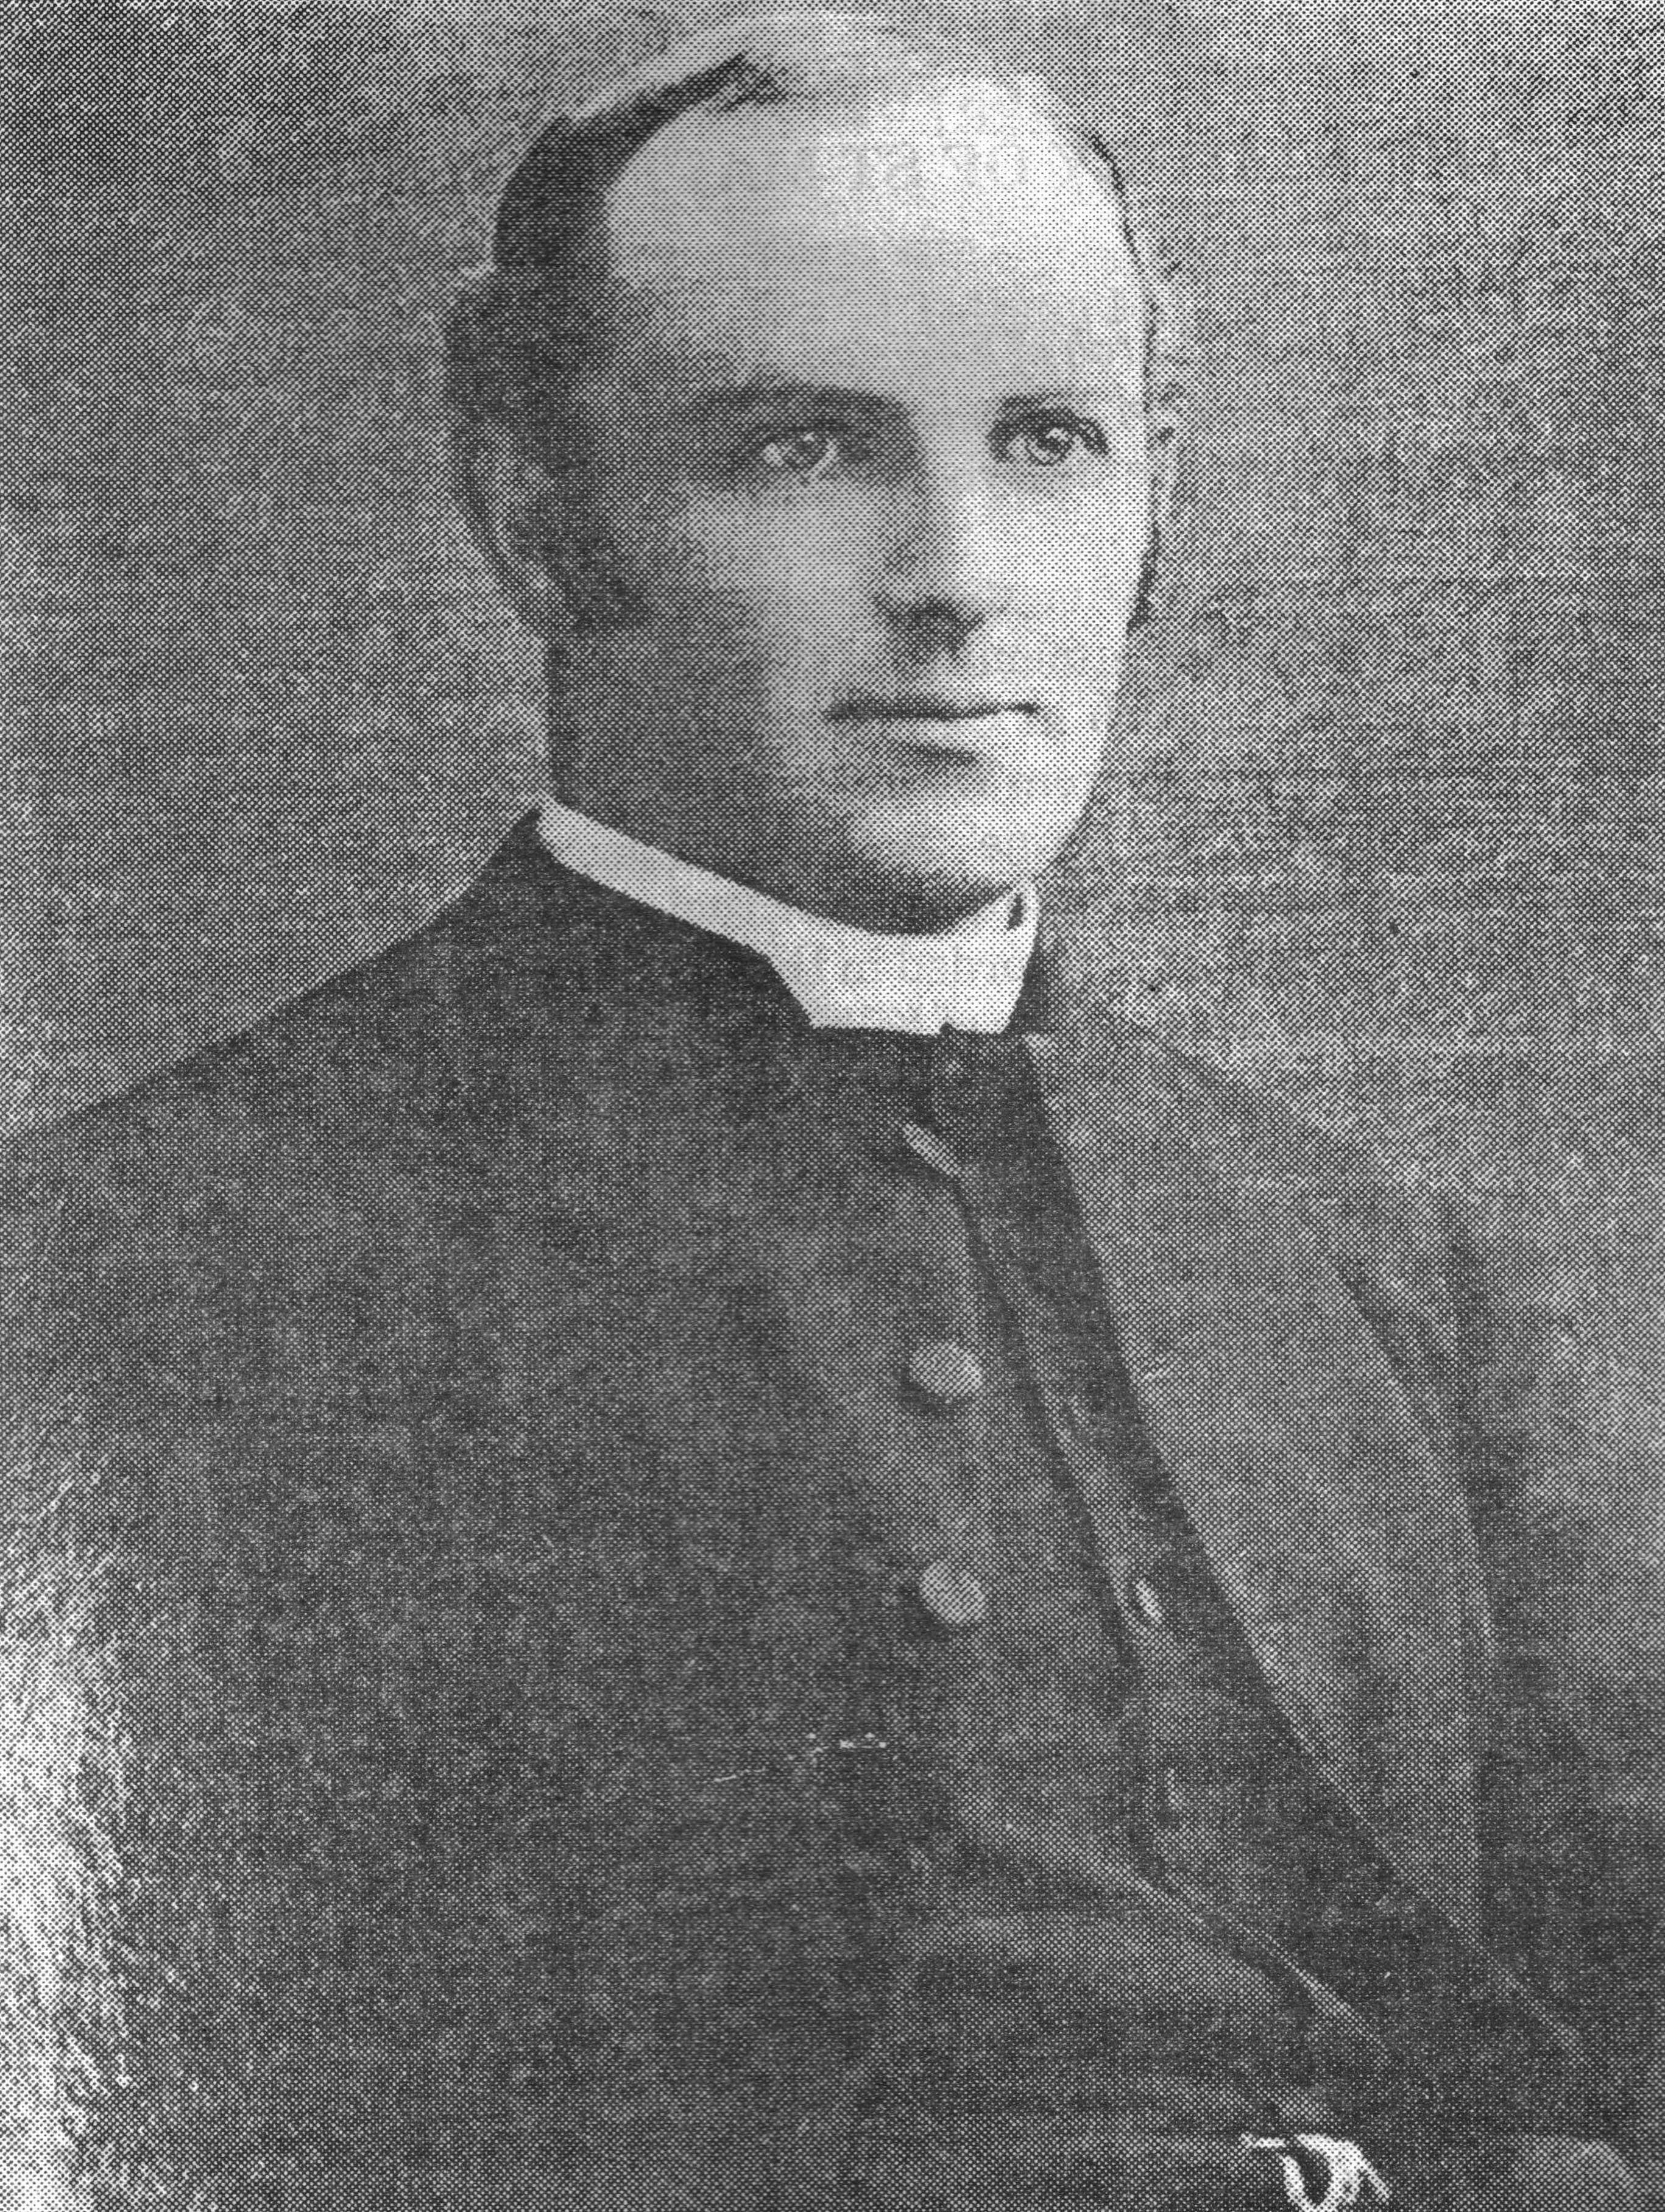
\includegraphics[width=.6\linewidth,center]{../images/RGTatham.jpg}
\caption{Rev R G Tatham}
\end{center}
\end{figure}


European settlement in the Murgon area commenced around 1846.\footnote{\emph{Wilderness to Wealth} Page 417 JE and EW Easton, \emph{Wilderness to Wealth} Page : being a history of the shires of Nanango, Kingaroy, Wondai, Murgon, Kilkivan and the Upper Yarraman portion of the Rosalie Shire, 1850-1950, Brisbane, WR Smith \& Paterson. 1950, repr.1974, p. 417} From the earliest days of settlement, well before the turn of the century, ministers from the Bush Brotherhood travelled long distances on horseback or horse-drawn buggy from Gayndah or Nanango to conduct services at the various homesteads. One of the earliest names is that of Reverend G J Tatham of Tiaro who ministered to the area around Murgon -- a mammoth task considering the distances to be covered and the associated travelling conditions to reach `the big squattages between Kingaroy and Tiaro'\emph{,} including Kilkivan. Rev Tatham is credited with having inspired the building of St Matthew's church in Kilkivan.\footnote{JE and EW Easton, Wilderness to Wealth: being a history of the shires of Nanango, Kingaroy, Wondai, Murgon, Kilkivan and the Upper Yarraman portion of the Rosalie Shire, 1850-1950, Brisbane, WR Smith \& Paterson. 1950, repr.1974, p. 417-418 \emph{Wilderness to Wealth} p. 417-418}

Established in the mid-1800s Barambah Station\emph{,} a property located between Nanango and the present township of Murgon, remains as a recognised landmark stopover for early explorers and travelling clergy alike. This ecclesiastical arrangement continued up until around 1903. The township of Murgon, as such, did not exist during these very early years, though intrepid adventurers were known to have travelled through the area in search of grazing land. With the development of a thriving timber industry, it is obvious that they noted the significant stands of harvestable timber.




\begin{figure}
\begin{center}
\includegraphics[width=1.\linewidth,center]{../images/timberHauling.jpg}
\caption{Delivering logs to the Murgon Sawmill}
\end{center}
\end{figure}


Regarding the church's development, a more formal worship arrangement appears to have begun around 1903 when the spiritual care of the infant township of Murgon was entrusted solely to the `indefatigable band of brothers from Gayndah, headed by the Ven. Archdeacon A R Rivers, whose curates, the Rev B P Walker and J L Puxley, passed through the infant township on their marathon horse rides'\emph{.} Gayndah Parish continued this arrangement for 10 years. When the Bush Brotherhood's base was moved from Gayndah and relocated in Charleville in 1913, the area was linked to the Nanango Parish. Murgon `was entrusted along with Goomeri, Boonara, Barambah, Proston and Overseas Settlement, to the spiritual care of Rev J H Steer, Rev C G B Turner and Rev C C H James, all assistant curates in Nanango.'

\section{The Coming of the Railway}

With the coming of the steam train era, rail transport played a major role in opening up areas for closer settlement in many areas of the developing world, providing, as evident in the burgeoning South Burnett region, an efficient method for transporting large amounts of produce such as gold and other minerals, timber to the larger mills, dairy products to milk, cheese and butter factories, plus moving livestock like cattle, sheep and pigs as required, as well as being a much faster means of human travel from one town to another.

The Queensland government finances were at a low level, `but the government realized that in order to generate wealth it was necessary to also spend it'\emph{.} Therefore, it embarked on a work-generating programme `through the construction of public buildings and, where it was both possible and expedient, the construction of a rail system'.\footnote{Tony Matthews\emph{, Landscapes of Change: a history of the South Burnett}, South Burnett Local Government Association, 1997 pp. 330-1} A branch line was constructed through the South Burnett. Commencing at Thebine the line to Kilkivan, a mining entre, was opened via Dickabram on 1 January 1886 and then on to Kilkivan on 6 December 1886.

A Royal Commission in 1889 recommended that the line be extended from Kilkivan to Nanango. It was opened progressively to Goomeri on 1 August 1902, to Wondai through Murgon on 14 September 1903, to Kingaroy on 19 December 1904 and Nanango on 13 November 1911. Branch lines were built from Murgon to Proston and Windera opening on 24 February 1923 and 28 March 1925 respectively and then from Kingaroy to Tarong on 15 December 1915.\footnote{Howard Quinlan and John R Newland, \emph{Australian Railway Routes} 1854-2000, Redfern, Australian Railway Historical Society (NSW Div), 2000, p. 43: Triumph of Narrow Gauge: a history of Queensland Railways, Brisbane Boolarong Press, 1990, rev 1998, pp. 109, 241.} The line to Kilkivan was constructed by McDermott, Owen and Company for \pounds113,634 and the extensions to Kingaroy and Nanango were built under the government's day labour program.\footnote{Commissioner of Railways Annual Report 1884-5, pp. 7, 133; 1901-2, pp. 73; 1903-4, p. 78.}

At first Murgon was a simple railway stop rather that a station. This initially was a flimsy tarpaulin structure to provide some `shelter for passengers and railway staff. The first station mistress was Mrs Easterby who also served as post mistress. The first permanent structure appears to have been a shed constructed to store meat, this building later served as the town's first post office' \emph{--} on the site where Murgon's modern post office now stands.\footnote{Queensland Railways Public Timetable 4 February 1907 and General Appendix.}
\balance

\printendnotes[custom]
\setcounter{endnote}{0}
\chapter{The Birth of a Town}
\nobalance

Early records refer to Mr George Arnell and his wife, Charlotte confirming them as significant persons in the history of both the township of Murgon and the construction of a centre for worship for the Church of England. A newspaper ``Chat'' with George Arnell in Brisbane's \emph{Daily Mail} newspaper recorded him as the earliest `living resident'\emph{,} having arrived in the district in July 1906, so his recollections are a valuable resource today. The opening of the railway on 14 September 1903 provided the impetus for the establishment of the township of Murgon from the cradle of a simple railway shed, as Arnell described it, which was the meeting place for the small though rapidly increasing community.

The first permanent selectors recorded in the burgeoning town area were loggers and bullock team operator, Jack Carey and the other, George W Nutt who called his selection \emph{Castra} and moved onto his holding in 1902 when the area was still feeling the effects of the severe federation drought. The Nutt family began farming and eventually progressed from a tin hut to a substantial home.




\begin{figure}
\begin{center}
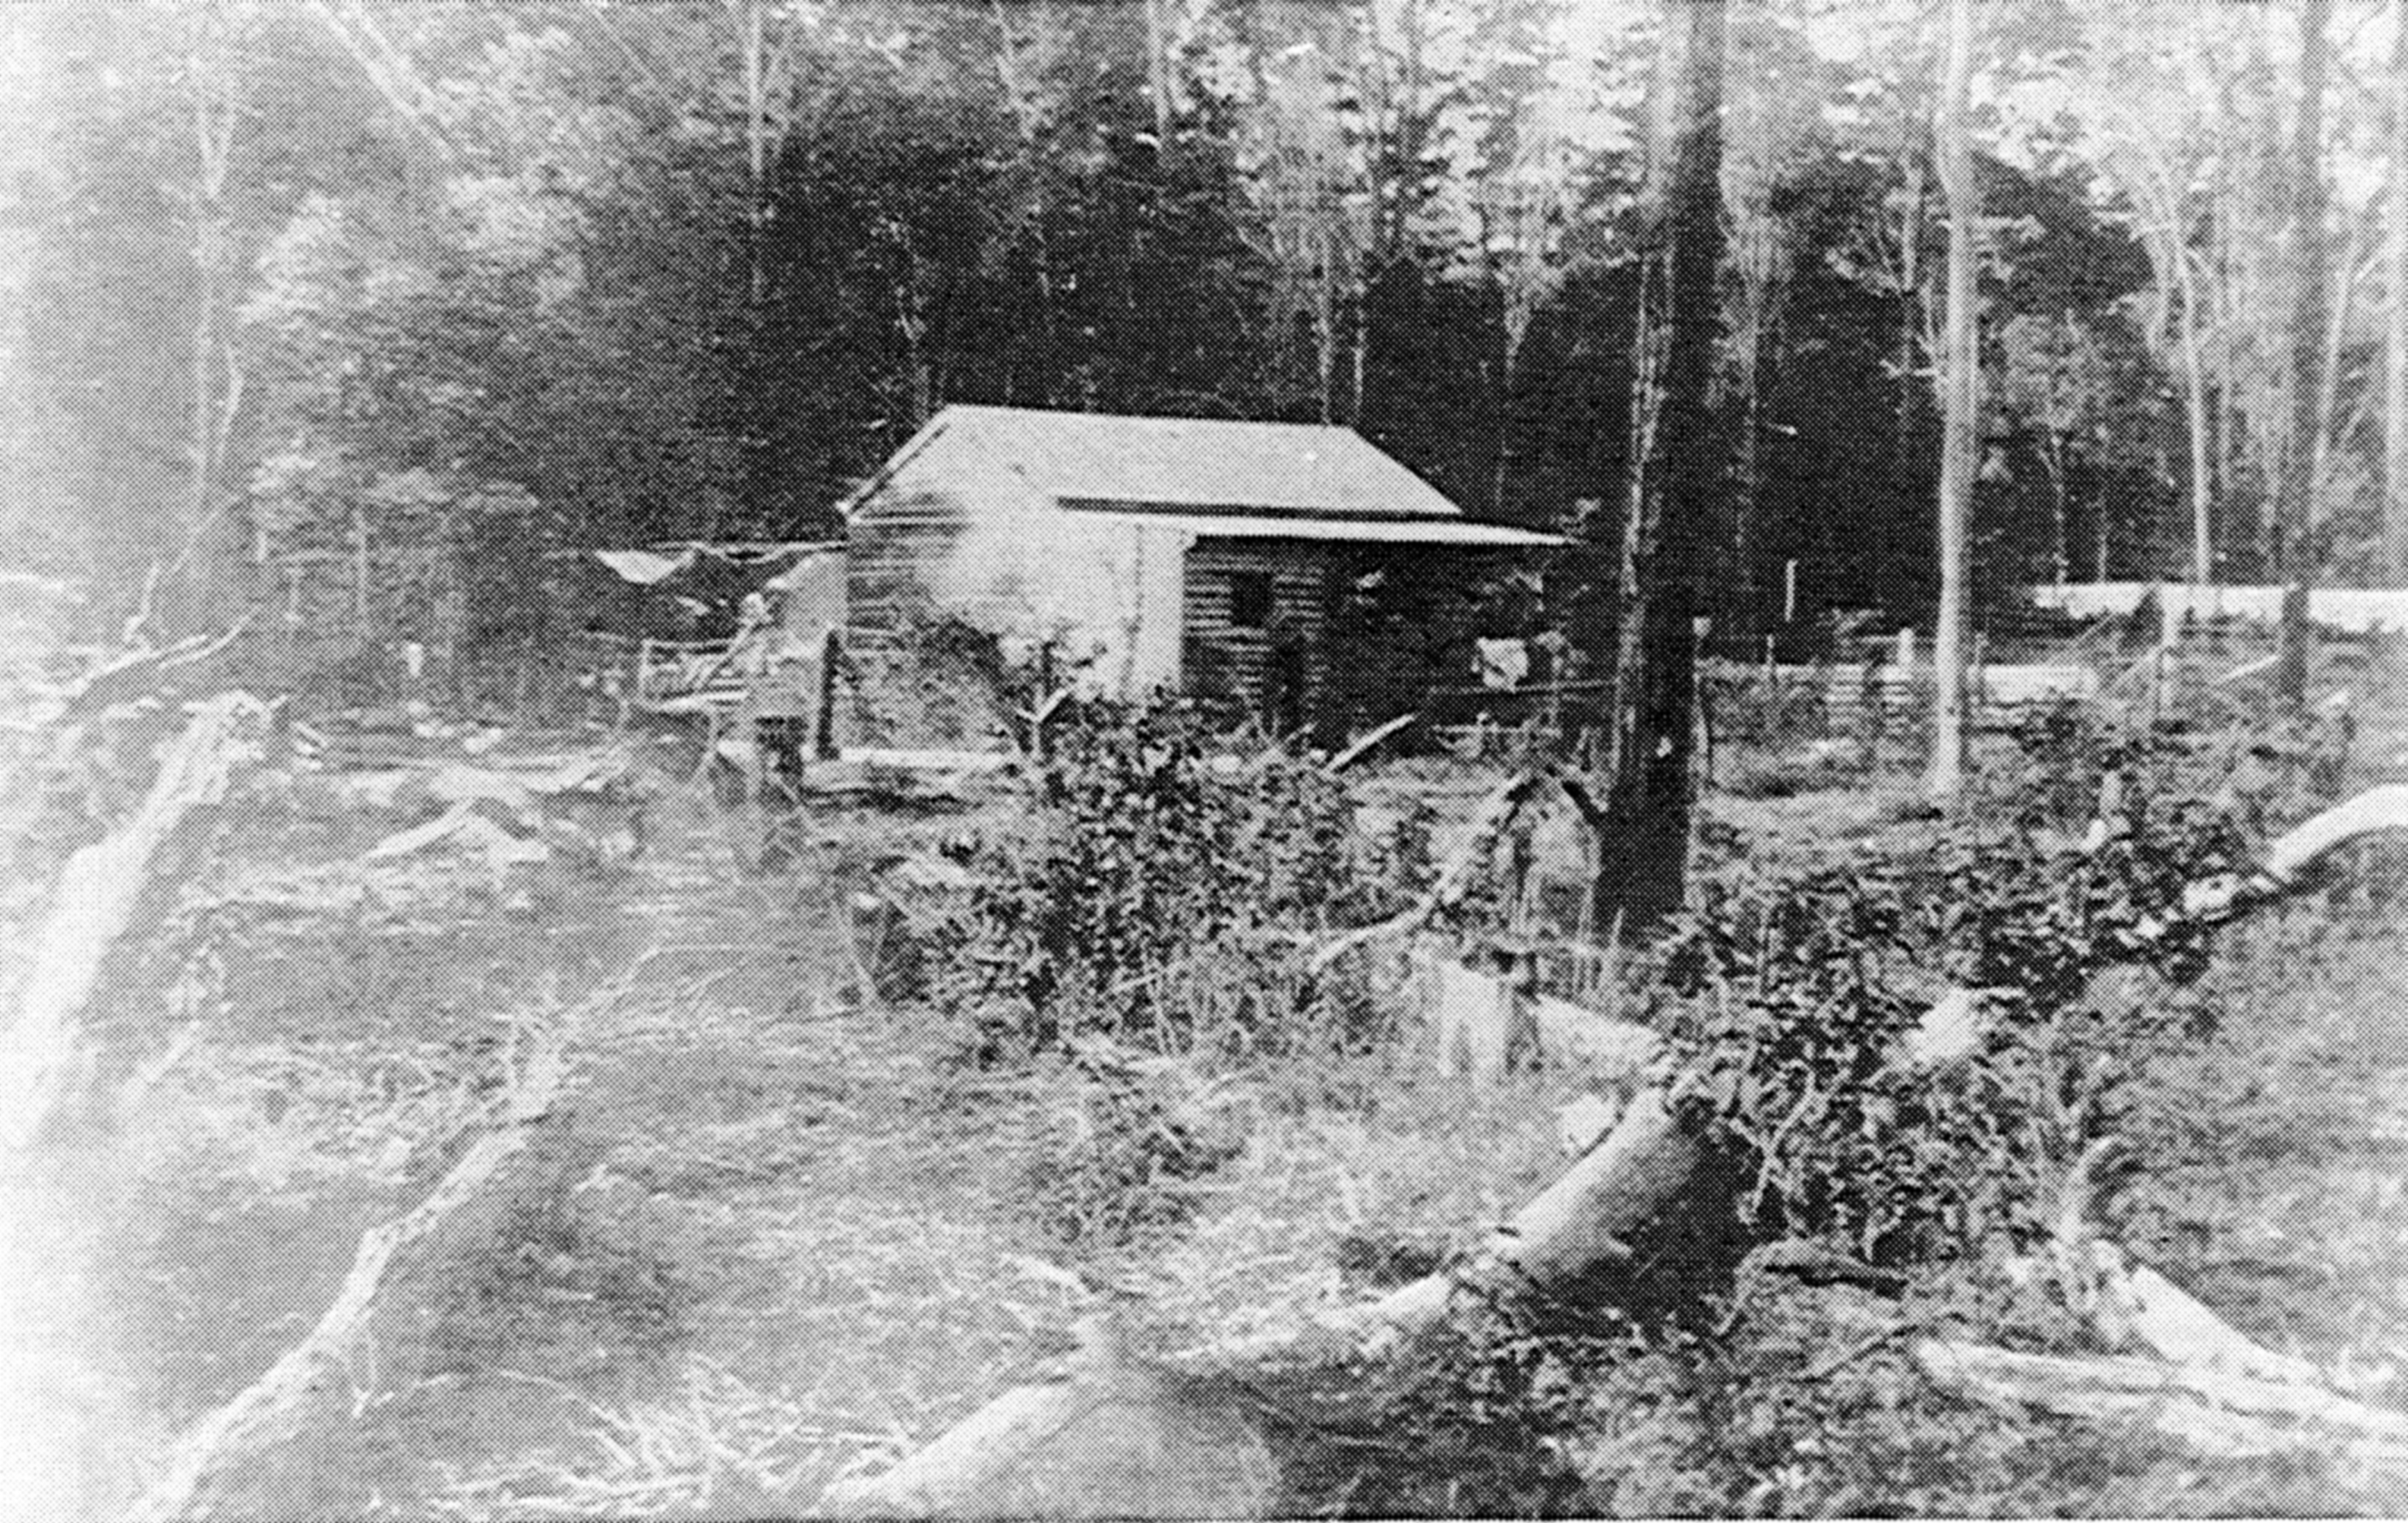
\includegraphics[width=1.\linewidth,center]{../images/HouseWNutt1908.jpg}
\caption{First home built by W. Nutt 1908}
\end{center}
\end{figure}


\emph{Castra} meaning \emph{Our~Camp} has come to be generally regarded as the first home built in Murgon in 1904 \ldots built by the Nutt family who were sawmillers in the area.\footnote{Tony Matthews, \emph{Landscapes of Change: a history of the South Burnett}, South Burnett Local Government Association, 1997, Vol. 1, pp. 395/6.} In February 1979, a \emph{South Burnett Times} article on page 12 indicates that, the then current owner of the home, Mr Cliff Krebs, offered it to the Murgon Shire Council for inclusion in the Murgon Dairy and Heritage Museum complex where it now stands, preserved as a local monument to early pioneering courage and a valued historical record for coming generations\emph{. Castra} has a beautiful crows ash timber floor and is tastefully furnished. Walking through~the door of \emph{Castra} is certainly stepping back in time and brings back many memories of how~it was `back then'.\footnote{\emph{South Burnett Times}, 7 February 1979, p. 12} \emph{Castra} now stands, with its history recorded, in The Murgon Dairy and Heritage Museum.\footnote{Murgon Dairy and Heritage facebook site.}




\begin{figure}
\begin{center}
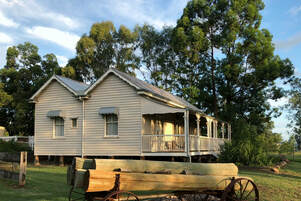
\includegraphics[width=1.\linewidth,center]{../images/castraOld.png}
\caption{Original Castra Building}
\end{center}
\end{figure}


As a further tribute to its significance, the name \emph{Castra} was attached to an Aged Care Facility built in Murgon next to Nutt Street. The original aging facility was sold to Southern Cross Care, Qld. demolished and replaced with a much enlarged and updated facility that was officially opened on March 2013 by Catholic Bishop Brian Finnigan before a packed room of invited guests.\footnote{https://southburnett.com.au/news2/2013/09/26/new-look-castra-opens-its-doors/}

Arnell's `Chat' indicates that the other early significant house in Murgon had also been built before survey and leased to early timber cutters (seemingly Jack Carey) or timber carriers such as Tom Ashton, Caleb Houghton and Granville Manthorpe, though he gives no official date for its actual completion. Consequently, it remains open to conjecture as to whether this house or `the more substantial \emph{Castra'} was completed first. Department records confirm that \emph{Heusil Barton} -- Lot 44 -- a substantial and larger home was leased from Caleb Houghton to Charlotte Arnell in 1906.

Following Charlotte's death in 1921 the property remained in the ownership of Trustees until 1936, though Granville Manthorpe again leased the property following her passing. A Manthorpe descendant married Mr Thompson of the firm Stewart and Thompsons, Murgon's drapers. After some time these partners went their separate ways to establish Thompsons the Mercers of Murgon and Stewarts Drapery who remained iconic traders in Murgon for decades following. The \emph{Daily Standard} article of 24 November 1923, named Charlotte's son-in law, Ronald Edwin Lever (married Dorothy Arnell), as executor and trustee of her estate. The property was subsequently sold to Norman Wilson Smyth on 23 August 1937. It stands as a functioning family home to this day. The Lever name remained prominent in Christ Church's history until recent times. Murgon's Stewart Heights is named for the Stewart family.




\begin{figure}
\begin{center}
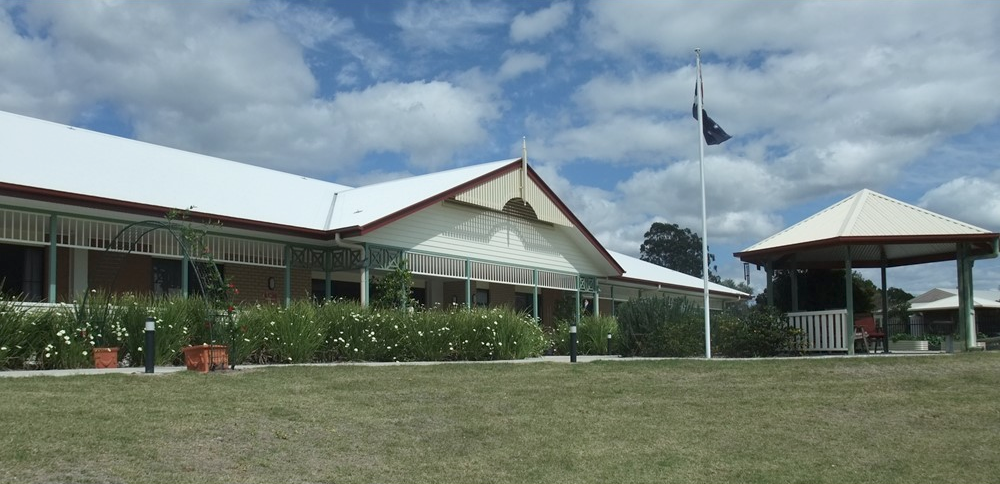
\includegraphics[width=1.\linewidth,center]{../images/castraToday.png}
\caption{Castra Today}
\end{center}
\end{figure}


The ``Chat'' continues:

\emph{`A portion of Barambah Station\ldots was resumed, and during 1906 these areas were thrown open for selection in the Wondai Lands Office. All the forest areas were selected, but very few of the scrub blocks were taken up -- the latter were reserved for `English settlers, or for home people'\ldots{} (Mr Arnell) selected 212 acres of land within sight of the railway station on the eastern side of the line\ldots{} (and later) purchased two other selections \ldots for dairying and farming\ldots(In his prophetic words) `Murgon is on the verge of big things.'}

The expansive width of Lamb Street, Murgon's main street, can be directly attributed to the harvesting of timber in the area in these formative years. Bullock teams were used as transport and needed plenty of space to manoeuvre with their precious cargo en-route to the rail head.

Realising the potential of the district the Murgon Progress Association was formed in 1906 with George Arnell as Chairman and with a membership of around 35. That first year also saw the establishment of Maddison's hotel, Angel's butcher's shop, Grey's grocery store and Witt's blacksmith's shop. Within two years the Association had secured 10 acres reserved for school ground purposes, reserves for show grounds, a mail service to Windera settlement 20 miles away, medical attendance at Barambah Settlement and a goods shed at the railway station.\footnote{`A Chat with George Arnell'\emph{, Daily Mail,} 18 April 1922, p.10}

Arnell's `Chat' has a section headed `Early Day's Benefactress', a Mrs F L Fick who, prior to the availability of doctors, pharmacies or any form or first aid or bush nursing, including midwifery, saw to these needs in the district (many of whom were Church of England) and {[}in Arnell's words{]} she was really the ``Mother of Murgon''. She is quoted as having `a good knowledge of medicines and first aid generally. Her services were frequently called upon \ldots{} she has been known to ride 30 miles on horseback through the night to attend some needy cases \ldots{} was looked upon as a general benefactress and although on the verge of 61 years (in 1922) still carries on the good work with successful results. For the first 5 years of Murgon, before the coming of a doctor, Mrs Fick had not one fatal case.'

The Fick family's property was located on the banks of Barambah Creek between Murgon and Wondai. The road bridge was built nearby to replace the former Fick's Crossing\emph{,} a natural shallower part of Barambah Creek. In later years, the large water hole and a portion of the original Fick property became a popular recreation area. Substantial facilities were constructed, and an area allocated as Fick's Crossing Park\emph{.} Used extensively over the years as a convention centre, out-door education centre, a venue for church functions and camps, swimming and canoe activities, and even Sun Girl and Miss Queensland beauty competitions. In more recent years it was utilized by Silver Wattle Foundation as an indigenous training centre for First Nation youth from the area. Lining centre for First Nation youth from the area.
\balance

\printendnotes[custom]
\setcounter{endnote}{0}
\chapter{A Permanent Place of Worship}
\nobalance

\section{1913--1914 : Rev John Howard Steer}

Nanango curate, Rev J H Steer, was entrusted with the care of Murgon and the surrounding area, from Wondai to Sexton including Boonara, Mondure, the small settlement at Murgon, and Kilkivan, until 1914. He travelled by horseback from Nanango.\footnote{\emph{A Tapestry in Faith --} St David's, Boonara, Centenary Booklet, 1914, pp. 11, 12.} Rev Steer diligently brought the various sacraments to central homesteads or private homes. For example, on 3\textsuperscript{rd} January 1914 he solemnized the marriage of Lilly Bull to Leonard Hatchett at ``Eailsdon'', the residence of Mr George Hatchett.\footnote{Personal Communication, Shirley Dennien, great grand-daughter.}




\begin{figure}
\begin{center}
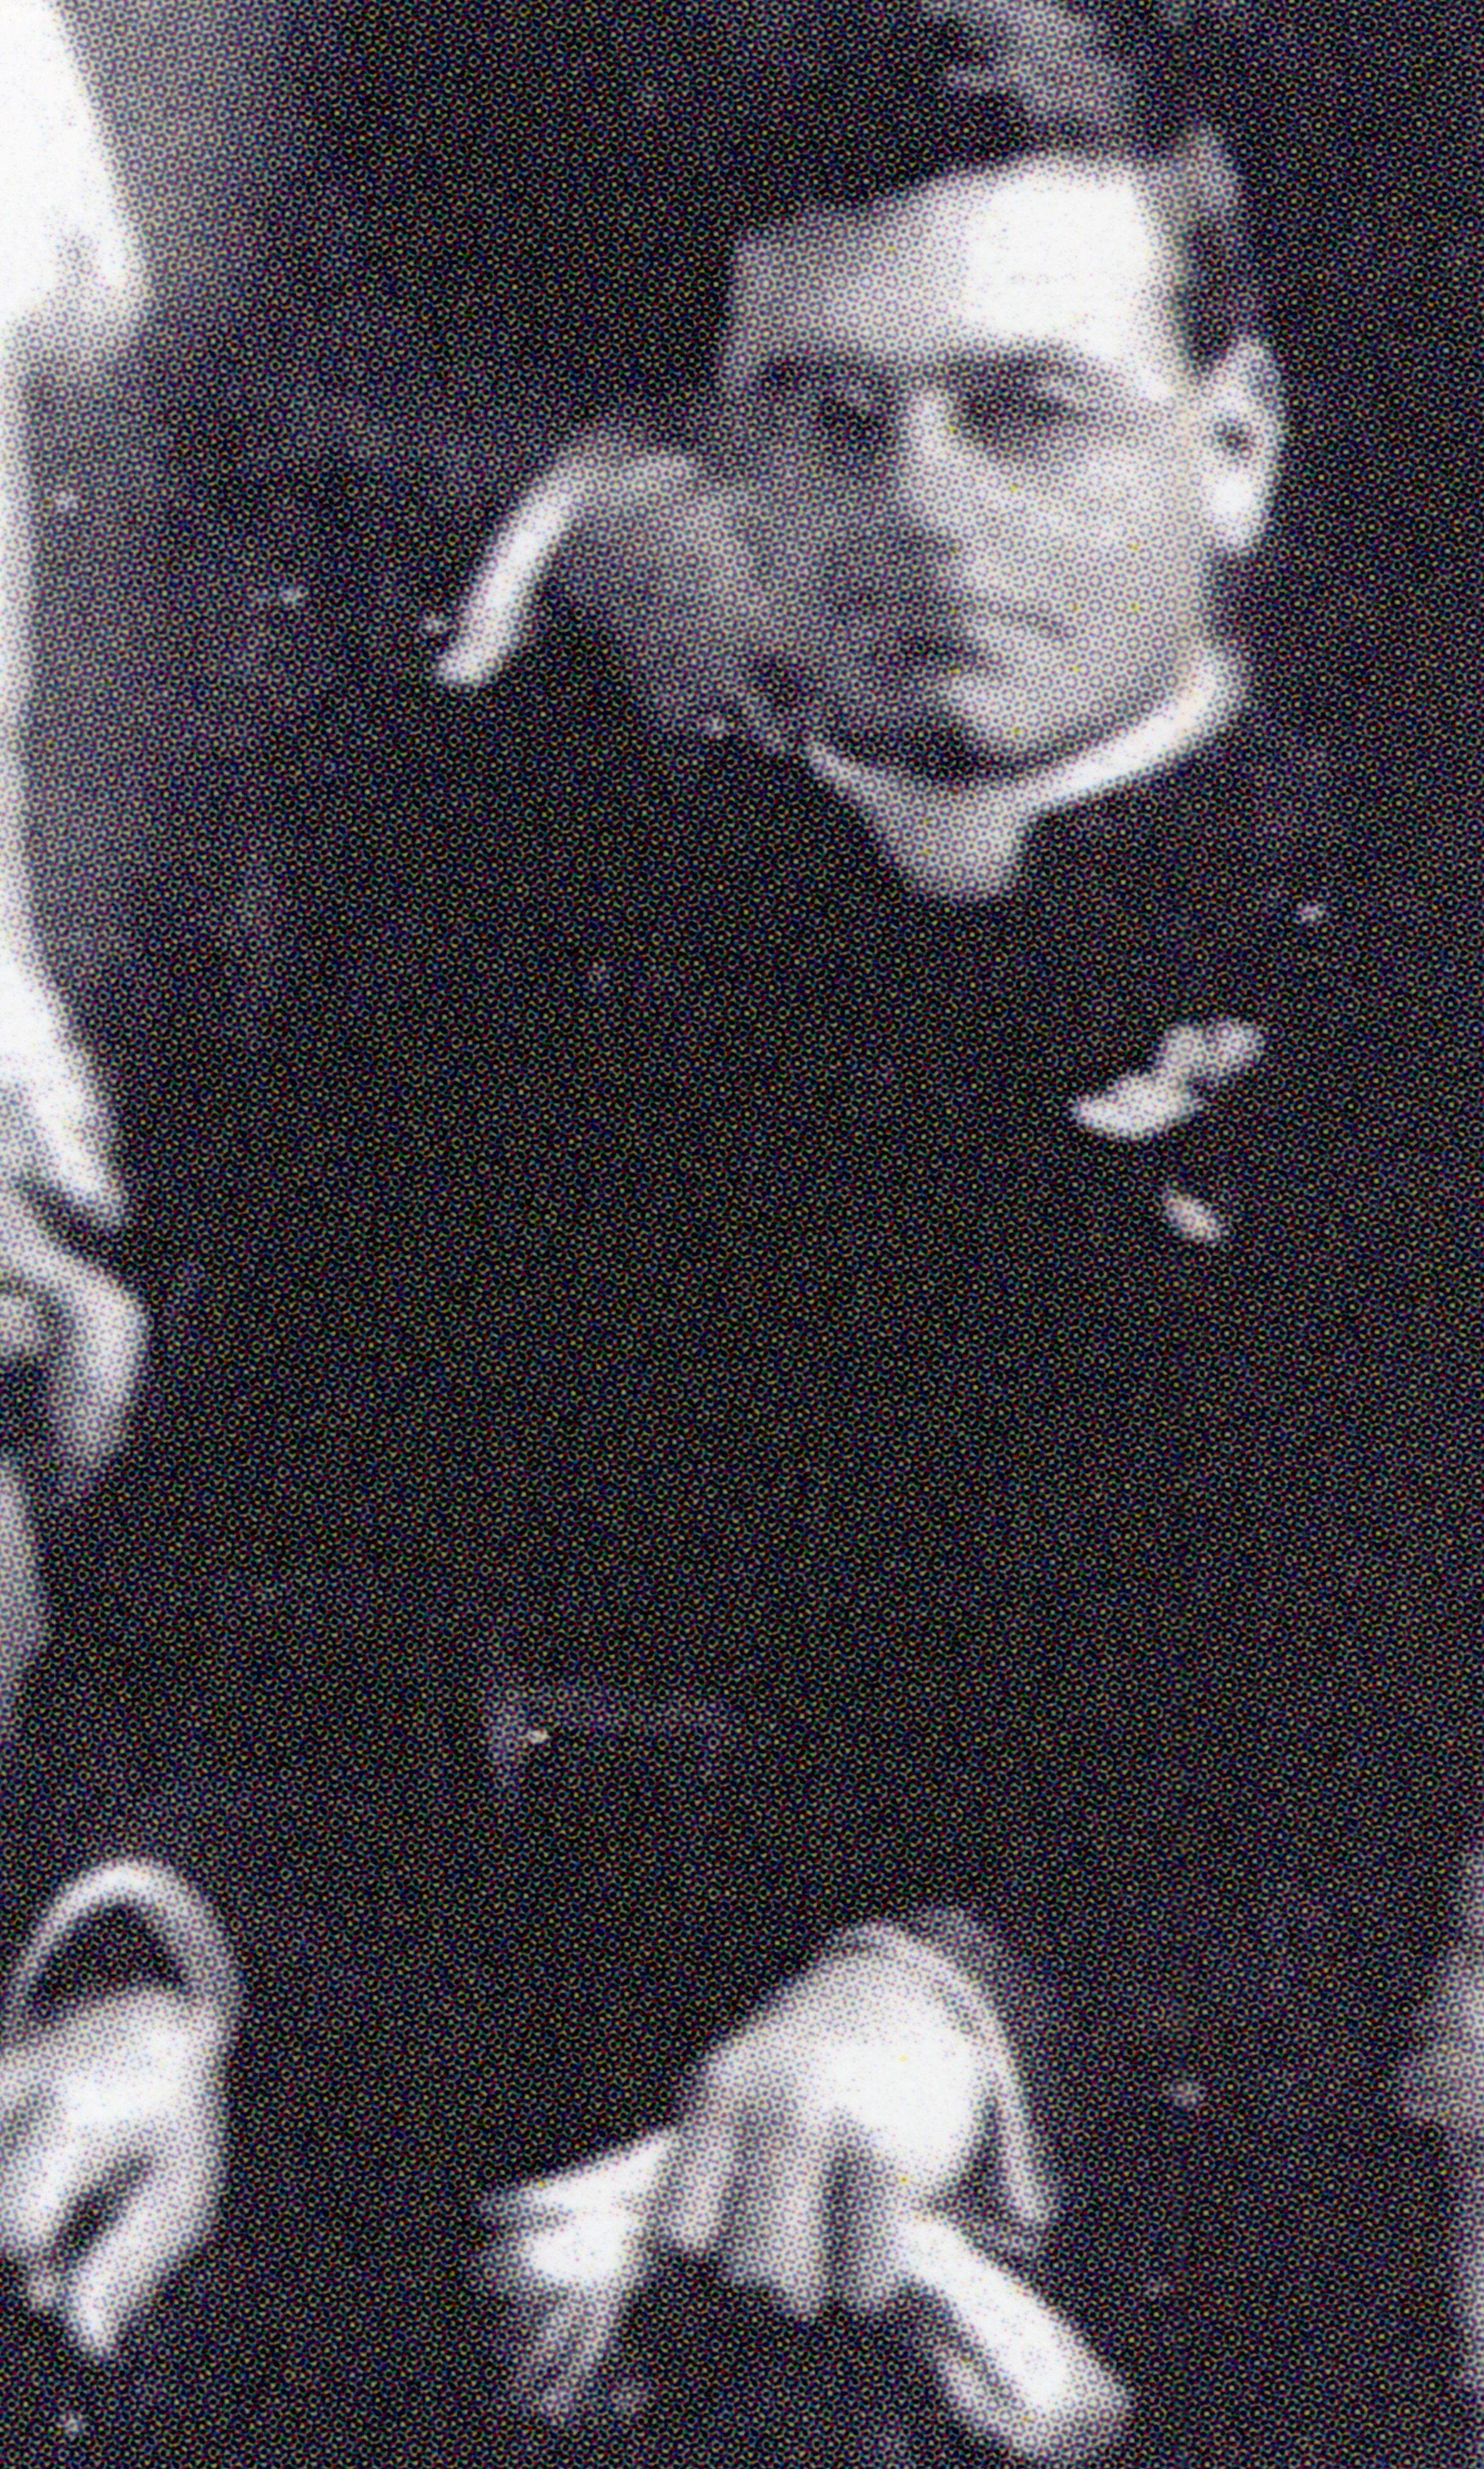
\includegraphics[width=.6\linewidth,center]{../images/JHSteer.jpg}
\caption{Rev J H Steer}
\end{center}
\end{figure}


Rev Steer is remembered as a great church builder. During his time in the parish, sites were obtained for three new church buildings. Boonara church opened in 1914. The new building swung into action, hosting its first wedding (Idalia Constance Nissen to Oscar Sidney Wallace) on 7 January with Rev Steer officiating. While construction of the current church building in Goomeri began during Rev Steer's incumbency, the completed Church of the Epiphany, was officially dedicated on 12 March 1916, by Archbishop St Clair Alfred Donaldson.\footnote{Parish of Kilkivan, \emph{Family Magazine}, June 1986 which carried a reprint of articles from \emph{Our Parish Magazine}, April 1916.}




\begin{figure*}[!htb]
\begin{center}
\includegraphics[width=1.\textwidth,center]{../images/hatchettBull1914.jpg}
\caption{Marriage of Lilly Bull to Leonard Hatchett, 1914}
\end{center}
\end{figure*}


When one considers that World War I was raging in Europe and that most of the settlers who had their ancestral roots firmly planted there, had family members in fighting overseas in support, it is a remarkable effort that the labour-strapped Australian settlers were able to bring two church buildings into being.

One of the earliest records of Diocesan involvement by parishioners from this area, is the nomination in 1914 of Richard Maudsley, a grazier of \emph{Undaban} and a parishioner from Boonara, as a synodsman for the 1915 Synod in Brisbane. An entry for Nanango Parish in the 1916 Year Book lists R Maudsley and E Schneider (Boonara) and I Moore (Goomeri) as Wardens for their centres. B Graham and R Maudsley are listed as Synodsmen.\footnote{Church of England, Brisbane Diocese, \emph{Year Book,}1919 - 1927.} Thus, it is evident that the Church of England had a strong and vigorous foundation in the whole district surrounding Murgon as well as in the town area itself.




\begin{figure}
\begin{center}
\includegraphics[width=1.\linewidth,center]{../images/RichardMaudsleyAndWifeMariaJane.png}
\caption{Richard and Maria Maudsley}
\end{center}
\end{figure}


\section{Smaller Dependencies}

Several small dependencies are mentioned as centres of worship in the early years. Some of these a recorded in small cameos in the Kilkivan Centenary Booklet.

\subsection{Cinnabar}

Cinnabar is named as the first centre outside Kilkivan. It is believed that services started as far back as 1898 and were conducted in the afternoon in the front room of the home of Mr and Mrs T Standen, their daughter, Grace, playing the piano for the hymns. In 1912 Rev Steer wrote an article on the 20 September celebration of the Standen's Silver Wedding anniversary. In 1925 the Cinnabar Hall was built, and services were held there. Mr Standen and, later on, Mr L Sempf were prominent in church activities and administrative positions. Regular church services at Cinnabar ceased in the early 1930s thus during Rev Lee Warner's incumbency.\footnote{St Mathew's Kilkivan\emph{, Centenary Booklet,} p. 24.}

\subsection{Fat Hen Creek}

Residents of Fat Hen Creek also held services, the first of these being held in 1921 during Rev Shand's time as vicar. Services were held in the local Rossmore school -- two per month, one Church of England and the other Methodist. Local resident, Mrs Waldock, conducted Sunday School in her Black Snake Road home, just over the hill from Rossmore school. Ministers sometimes stayed overnight at the home of Mrs A Dimock. Church Chronicle notes of April 1937, when Rev Lee Warner was vicar, mention the Rossmore Ladies Guild. Service ceased in 1942, most likely as a result of war-time petrol allowance restrictions which hindered Rev Griffith's travels.\footnote{St Mathew's Kilkivan\emph{, Centenary Booklet,} p. 26.}

\subsection{Woolooga}

Rev Steer conducted regular services at Woolooga in the original (old) hall from 1913 although services and weddings had been conducted in private homes for many years prior. During Rev Eglinton's time as vicar, the September 1930 Parish Notes recorded that land for a church on a `prominent and valuable site' which Diocesan records describe it as `Vacant land. Subdivision Two of Portion 152, County Lennox, Parish of Brooyar, given by R C Hall of Woolooga about 1931 for use as a church'.

There were optimistic ambitions for a church and vicarage and apparent great faith in the future of the area. A committee was formed with office bearers named as `Mr R C Hall, J McMullen (school teacher), and George Wilson (station master). Plans were drawn under the guidance and advice of Archdeacon Glover with details of timbers to be used in its structure and for finishing details. Financial assistance was sought through Diocesan channels. However, this was not forthcoming due to `the stringent state of diocesan finances.\footnote{Diocesan Correspondence files, Diocesan Archives, Brisbane.} Sadly, their optimism did not bear fruit. The church was never built and services were discontinued in 1933, when Rev J Lee Warner was vicar.\footnote{St Mathew's Kilkivan\emph{, Centenary Booklet,} p. 25.}

By 1965, following a letter from Kilkivan Shire Council's Mr E Keating regarding possible foreclosure due to overdue rates of \$12.93, serious consideration was being given to selling the site, Diocesan advice the parish wardens was that , `If Mr Hall is still alive, we would like you to obtain his views on a proposed sale.' Finally, in 1971, following the parish's formal application through its parish secretary, Mr Frank Horrocks, for `permission to sell' the land to Mr J H Cullis (Cullen?) for \$40, the land passed out of church hands.

From 1905 to 1912, clergymen from St Andrew's One Mile, Gympie provided services for Sexton Anglicans, on their way to Kilkivan. Minutes of a meeting on 15 March 1911 show that the parish was willing to pay \pounds7/10/- for a horse for the curate, Rev J H Steer. Mr Steer transferred to Nanango in 1913 and owing to boundary changes, Sexton was still in his area. Services were held in Carmyle School (at its original site). Mr Dave Culley was a warden. Rev Lee Warner is credited as asking for Sexton and Woolooga go be transferred back to Gympie,\footnote{St Mathew's Kilkivan\emph{, Centenary Booklet,} p. 28.} however, this did not eventuate.

\section{1915--1919 : The Great War}

During these troubled years, curates from Nanango, including Rev C G B Turner and Rev C C H James\emph{,} had the option of a `push bike' -- apparently, a short-lived venture.\footnote{St Mathew's Kilkivan\emph{, Centenary Booklet, p. 6}} In Murgon, church services were held irregularly in the home of George and Charlotte Arnell. Later they were conducted in the Salvation Army Hall. Caleb Houghton's name occurs as a Salvation Army Officer.\footnote{Personal Communication, Jeff and Muriel Schultz, Murgon residents.}




\begin{figure}
\begin{center}
\includegraphics[width=1.\linewidth,center]{../images/SalvationArmy.jpg}
\caption{Back (l to r): Colour Sergeant James Sommerville, CMS Caleb Houghton, Seated: Kate Harvey, Mrs Sommerville, Mrs Houghton}
\end{center}
\end{figure}


\section{1919--1922 : Rev Rupert Warner Shand}

In the years immediately preceding the arrival of Rev Shand, the support for a permanent Church of England worship centre in Murgon gained momentum, coinciding with a proposal for separation from Nanango Parish. A separate parish for the area called The Parochial District of Murgon was officially formed on 1 February 1919, comprising Murgon, Wondai, Mondure, Sexton, Abbeywood, Silverleaf, West Goomeri, Kilkivan, Boonara, Goomeri, Cinnabar, Fat Hen Creek and Barambah Mission.\footnote{Church of England, Brisbane Diocese, \emph{Year Book,}1919 - 1927.} Shortly after this, Archdeacon Rivers was entrusted with the task of defining the parish boundaries to include Tingoora, making a total of 14 dependencies under his ministry.

At the time Rev Shand took up his position as vicar of this new parish the Parish Burial Register's very first entry reads `\emph{1. Ethel Maria McIntosh, Boonara, Goomeri -- Married Woman -- (Age) 19 -- died 23 January 1919, buried 24 January 1919.'} Ethel was the daughter of Richard and Maria Maudsley, \emph{Undaban}. Robert and Ethel's first child, Joyce Ethel McIntosh was born at Murgon on 16 January 1919. Ethel did not recover from the birth and she died a week later, on 23 January 1919.




\begin{figure}
\begin{center}
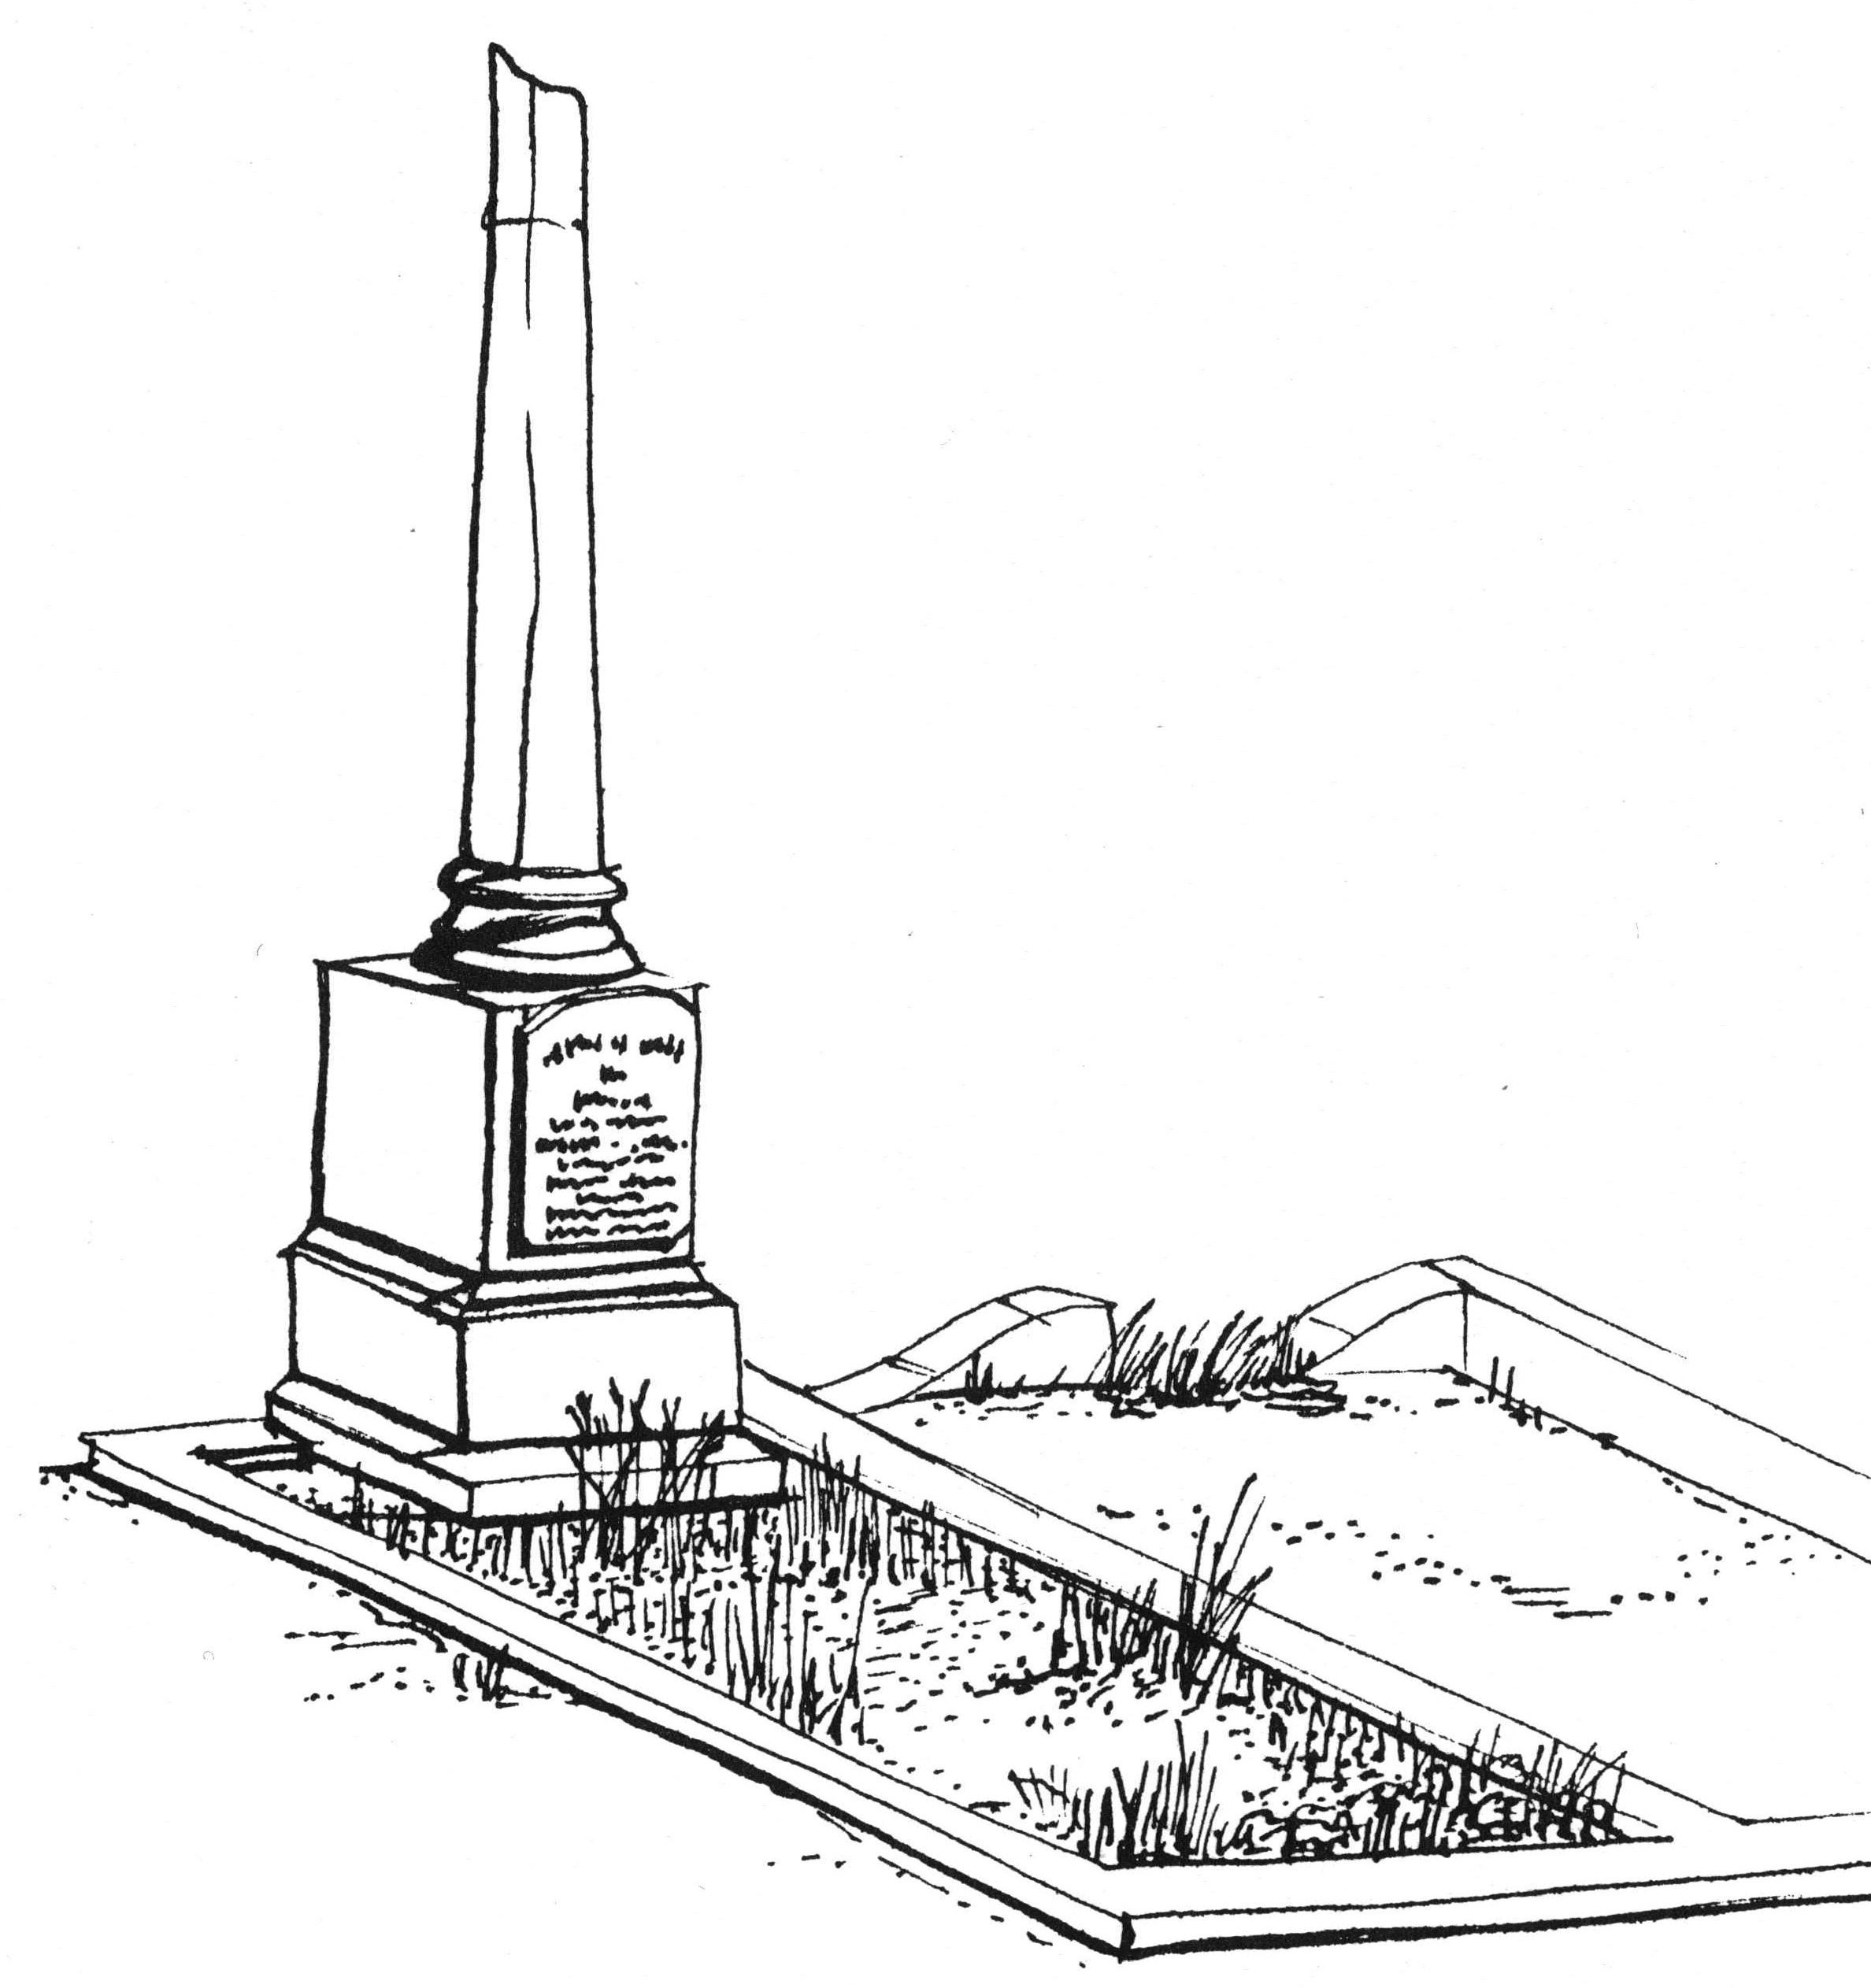
\includegraphics[width=1.\linewidth,center]{../images/graveOfEthelMcIntoshInGoomeriCemetery.jpg}
\caption{Grave Of Ethel McIntosh In Goomeri Cemetery}
\end{center}
\end{figure}


Following a service conducted by Reverend Rupert Wagner Shand in Goomeri's Church of the Epiphany, she was buried at Goomeri Cemetery. Her headstone is topped by a broken column indicating that she died in the prime of her life.\footnote{\emph{Ordinary People Extraordinary Lives,} p. 357; Drawing of Grave and Headstone or Ethel McIntosh -- Courtesy Janine Seltzer.} Entry 2 lists the funeral of James Henry Black (45) of Murgon, died 27\textsuperscript{th} and buried 28 January 1919. Thus, Rev Shand's services were called upon as soon as he arrived and prior to the official formation.

A house, originally built in Gympie was demolished and re-erected in Murgon, then rented as a vicarage for the Rev R W Shand.\footnote{JE Murphy and EW Easton, \emph{Wilderness to Wealth: being a history of the shires of Nanango, Kingaroy, Wondai, Murgon, Kilkivan and the Upper Yarraman portion of the Rosalie Shire, 1850-1950}, Brisbane, WR Smith \& Patterson, 1950, repr. 1974, p. 418. \emph{Wilderness to Wealth}, p. 418.} The first meeting of the Parochial Council was held in this residence on Tuesday, 11 February 1919 at 8 p.m.\footnote{Anglican Church Southern Queensland, Diocesan Archives, Murgon Parish Minutes, DJ Box 3.} Attendance is shown as Messrs Pimlott, McDonald, G Black, J Faunce, L Smith, G Willis and C E Baldwin -- names that have remained synonymous with the formation of the parish.

Items dealt with included the basic requirements for the running of the parish: set of books for recording purposes, the opening of a Queensland Savings Bank account for the Parochial Funds, the appointment by consensus of a warden (Mr Pimlott is named) and a treasurer to oversee the running of the parish until the more formal arrangement of nominations and election at the Easter Meeting (a general meeting of parishioners). The suggested allocation of monetary contributions from the various outlying centres was to be communicated to the various centres by circular letter.

The vicar was delegated to \emph{`}meet with the ladies in connection with the forming of a Society of the Treasury to canvass the town and district\emph{'} Thus, from the very first meeting the tradition of utilizing the value of women in the mundane duties of raising monies for parish funds was clearly recognized.

At this first Parochial Council meeting Warden Pimlott (Mondure) moved: that the Council is of the opinion that for the proper working of the Parish a motor car be purchased and that parishioners be appointed with regard to guaranteeing or otherwise -- a quite remarkable and commendable decision in these early post-war years. It was seconded by Mr McDonald. The purchasing committee comprised Messrs McDonald, Faunce and Smith. This was followed up at the March meeting with a request for all centres to actively engage in raising funds for this purpose. From the very beginning, the matter of adequate finance years was prominent at all council meetings. The 11 March meeting resolved that the stipend be \pounds20-16-8 and that a sum of \pounds50/year be paid for the vicar's traveling expenses.\footnote{Anglican Church Southern Queensland, Diocesan Archives, Murgon Parish Minutes, DJ Box 3}

The Easter (or Annual General) Meeting was held on the evening of 8 May 1919 in the Murgon School of Arts, Archdeacon Rivers in the chair. Rev Shand gave a glowing report of progress in the first two months and in the absence of treasurer Mr Jarvis, his report was presented by Mr Standen who formally moved its adoption. Mr Pimlott was appointed Vicar's warden with Mr McKell confirmed as Peoples Warden from six nominations. The Parish Council consisted of Wills, Winter, Baldwin, Crocker, and Haig and Vicar's Appointments -- Messrs James, Faunce and Standen

New Parochial Council members appointed to positions were Mr Jones (treasurer); Messrs Hampshire and R Maudsley as synod representatives - Mr Maudsley having been in this position since his appointment in 1914.

The revised assessments for each centre were: Murgon \pounds64; Kilkivan \pounds53-10-0; Boonara \pounds40; Wondai \pounds35; Mondure \pounds58; Sexton \pounds12; Overseas \pounds12; Tingoora \pounds12\textbf{.} For a grand total of \textbf{\pounds326-10-0} for the Parish.

It appears the church was carrying an overdraft as a motion to form a committee to reduce same was put and carried.

Diocesan records confirm that the `tyranny of distance' continued as a very prominent issue in the early years of settlement, with horses playing a significant part, though subsequently supported by the use of push bikes and even a motorcycle.\footnote{St Mathew's Kilkivan\emph{, Centenary Booklet.}} It remained so as Rev Shand began his ministry in Murgon.

The August Parish Council Minutes included Rev Shand's list of expenses; Horse hire 5/-; Benzine \pounds1-1-0; Repairs 16/-; Season Tickets \pounds1-13-6; for a grand total of \pounds3-15-6.

Progress in the transport area underwent a great leap forward with the vicar's purchase of a model T Ford, `affectionately' known as a `Tin Lizzie', or, more likely, Model A - a great improvement on the `T'. The motor vehicle was acquired for \pounds165, terms being \pounds75 deposit with the balance in to be paid in instalments. Monies for this upgrade came in part from the vicar's proactive sale of a motorcycle for \pounds27-10-0 and Sulky and Harness for \pounds18-0-0. More money-raising efforts were discussed at length with a decision taken to hold a Ball in September with proceeds to a Car Fund -- tickets 5/- and 3/- and two representatives were a appointed from each centre to guarantee their quota required for the purchase.




\begin{figure*}[!htb]
\begin{center}
\includegraphics[width=1.\textwidth,center]{../images/TouringCarParkedOutsideTheWaldockResidenceMurgonca1920s.jpg}
\caption{Touring Car Parked Outside The Waldock Residence Murgon ca 1920s}
\end{center}
\end{figure*}


Apart from recording relevant official details, the services register often contained interesting facts which throw light on the often harsh conditions under which these ministers toiled. One such early entry notes: `No Service, rode horse, roads awful!' I imagine the poor man would have felt rather frustrated that after making such an effort, no one else turned up. A little later he recorded `Very wet. No Service', and again a little further down, `Creeks flooded'. 12 November 1919 services register again endorsed the actions of Rev Shand in purchasing a replacement car for \pounds215 -- a confirmation of the effect of poor the condition of roads and the general travel conditions of the day.

Even with all the difficulties presented to the vicar and his flock, a choir had been mustered in Murgon and regular practice meetings were held. The 12 November 1919 minutes record a resolution `that choir practice be withdrawn from the School of Arts and that the chairman arrange a place of practicing'. No explanation for the move was recorded.

Great steps forward had been achieved in this short eight-month period and the wheels of progress continued to gain momentum. Plans and specifications were drawn by architects, WH Atkinson, Adelaide Street, Brisbane. An article about calling tenders for construction of the church appeared in the \emph{Maryborough Chronicle, Wide Bay and Burnett Advertiser} on 7 August 1919 and the advertisement calling the tenders on 8 August 1919:

\emph{TENDERS are called for the ERECTION and COMPLETION of proposed CHURCH OF ENGLAND, MURGON (labour only). Lowest or any Tender not necessarily accepted. Tenders close SATURDAY, 23 August, 1919. Plan and Specifications may be seen at MR.W. R. CLARKE'S, Newsagents Agent, Murgon. Tenders to be addressed to W. H. PIMLOTT, Secretary Building Committee, Box 68,} \emph{Murgon.}




\begin{figure*}[!htb]
\begin{center}
\includegraphics[width=1.\textwidth,center]{../images/churchPlansSide.jpg}
\caption{Church Plans -- Side Elevation}
\end{center}
\end{figure*}





\begin{figure*}[!htb]
\begin{center}
\includegraphics[width=1.\textwidth,center]{../images/churchPlansSection.jpg}
\caption{Church Plans -- Sections}
\end{center}
\end{figure*}


Sourcing land at an affordable price was proving to be a stumbling-block. Most generously, George Arnell purchased and donated the land for the building of this much anticipated Murgon Church of England. A bank loan was taken out to cover building costs. `Dick' Maudsley (nephew of the previously mentioned, Richard) signed an agreement to `go guarantor'. From the Maudsley Family history, the picture emerges of a very hard working and generous man.\footnote{\emph{Ordinary People, Extraordinary Lives}, p. 143} Although his purchase of one of the first motor cars in the area earned him the unkind title of `Flash Dick', his open-handedness and faith through this sharing his prosperity were then clearly revealed. Local bank manager and church member, Mr Skyring, on learning of his decision, in obvious dismay, anxiously confronted Mr Maudsley. ``How on earth did you let yourself get talked into that, Dick?'' and was told, ``It's for the Church. It is all OK!'' Though no amount is mentioned here, later evidence reports estimated cost at \pounds900.

The builders, Wills and Haigh, commenced construction work very promptly.\footnote{Christ Church Parish Council Minutes, May 1920. (Diocesan Archives DJ 3 Box 3)} Everything was `by hand', from the sourcing of mill logs in the local area and the milling of same to the coal-face jobs of digging trenches and post holes with crow-bar and shovel, hand-sawing every board piece as required, to the hammering in of every single nail. When one takes into account that this is the period immediately following World War I and amidst an influenza pandemic and remembering the shortage of labour and materials, the progress of building works was astounding as recorded and confirmed by entries in minutes. Everything purchased was let to tender even to basic items such as the supply of nails.

In the short one-month period from the calling of tenders in early August the work had progressed to a point where the next important milestone could be celebrated. On 9 September 1919 Archbishop Donaldson `crowned the foundation block of the Murgon's new church. It is anticipated that the church will cost about \pounds900, provision being made for future enlargement.'\footnote{Anglican Church Notes printed in the Brisbane \emph{Telegraph,} 13 September 1919, p. 16.} For the remainder of September the vicar was away on leave of absence.'\footnote{Church of England, Brisbane Diocese, \emph{Year Book,} 1919 -- 1927 and the Service Register.} These visionary and intrepid early movers and shakers are to be congratulated for their foresight, dedicated support and faith for the remarkable achievements of 1919.

Of note is the marriage of Clarence Edward (Jack) Morgan to Daisy Ellen Bull (sister of the afore- mentioned Lilly (Bull) Hatchett) on 10 September 1920, again at her parents' Abbeywood home, just one day after celebrating the church's stump-capping a century ago. Rev Shand performed the ceremony.




\begin{figure*}[!htb]
\begin{center}
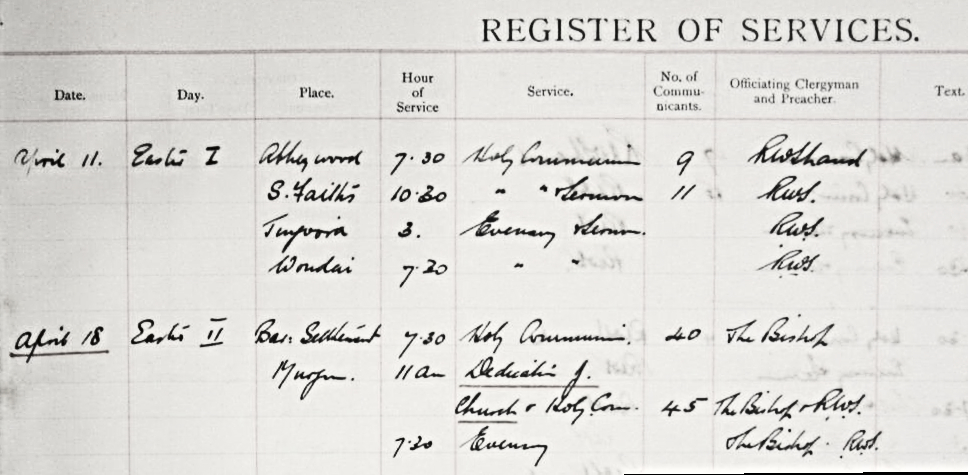
\includegraphics[width=1.\textwidth,center]{../images/dedicationByBishopLeFanu.jpg}
\caption{Dedicated by Bishop Le Fanu}
\end{center}
\end{figure*}


As the building process neared completion, a date for Christ Church's dedication was set and a call went out to parishioners for funds to employ further labour for a last-minute push. The volunteers who gave so promptly and generously in time, energy and dedication, through both on-site and behind-the-scenes support, are to be congratulated for bringing this major project so speedily to fruition. The building was completed in record time and dedicated by Bishop Le Fanu on Sunday, 18 April 1920 in the presence of a large congregation from all parts of the district. The church was reported to be `commodious and decidedly attractive in appearance, both externally and internally. After the dedication service luncheon was provided by the Women's Guild and the annual Easter Meeting was held.'\footnote{Brisbane \emph{Telegraph,} 24 April 1920 p. 10.} Thus, Mr Maudsley's generous and seemingly (in some eyes) rash decision was totally vindicated.




\begin{figure}
\begin{center}
\includegraphics[width=1.\linewidth,center]{../images/georgeAnneWaldock.png}
\caption{George and Anne Waldock}
\end{center}
\end{figure}


One of the attractive internal fittings was a silky oak altar and altar rails hand crafted and provided for the new church building by local citizen, George Waldock Jnr, (son of Nick Waldock, one of the earliest blacksmiths in Murgon) who continued in his father's trade. Although later replaced by an ornately carved altar, Waldock's generous and attractive altar remains in active worship service within the parish as the altar in St David's church, Boonara.\footnote{Ross Waldock's information re the altar by Geo Waldock.}

A successful flower show was held in early December 1920 over both afternoon and evening, in Murgon as a fundraiser, in aid of the Church of England with exhibits coming from Tingoora to Kilkivan, thus from all areas of the parish.

It noted the `wonderful display of flowers'\emph{.} There was an extensive list of categories for individual varieties including seven sections for various coloured roses, plus Chrysanthemums, Cactus Dahlias, Carnations, Asters, Cannas, Phlox, Stocks (single and double), Verbenas, Petunias, Nasturtiums, Dianthus, Sunflower, Gladiolus, Sweet Peas, Gerberas, and various flower collections, even including `Wildflowers' (which would have included Paper Daisies which were plentiful in the area). The prize for best head of Sunflower was awarded to Mrs R W Shand.

Other sections included a Pot Plant section, various forms of bouquets, floral bowls and artistic displays and a very extensive sections for vegetables, locally grown fruit, eggs, butter (salted and unsalted) which were all very well supported.

As usual with country affairs, there was a huge baking section, many and varied handcrafts such as knitting and crocheting and drawn thread work. Artwork included water and oil paintings, sketching, photographic section (landscape and portrait) and wood carving.

The children were not forgotten either, with schoolwork such as mapping, school exercise book, handwriting, artwork, dressed doll, sewing items including samplers and a garment made by a child.

Takings from the Flower Show amounted to \pounds60 -- a very satisfactory result. A dance in the evening terminated a very successful event.\footnote{\emph{Daily Mail,} 11 December 1920, p. 4.}This event seems to foreshadow the subsequent Agricultural and Horticultural Show Societies so popular in these rural towns.




\begin{figure}
\begin{center}
\includegraphics[width=1.\linewidth,center]{../images/waldocksBlacksmithShopMurgon1913.png}
\caption{Waldock's Blacksmith Shop, Murgon, ca. 1913}
\end{center}
\end{figure}


The Parish of Murgon records show a total of 14 centres being served, including St George's Tingoora and its dedication on 3 April 1921, though inclusion in parish activities occurred at least as early as 1920 as the above article indicates.\footnote{Church of England, Brisbane Diocese, \emph{Year Book,} 1919 -- 1927.}

Diocesan Records contain a type-written letter dated 05 April 1921, (as below), indicating Rev R Willand served during Rev Shand's period of incumbency and the exponential growth in the parish during this period.\footnote{Anglican Church Southern Queensland, Diocesan Archives, Murgon Parish Correspondence.}

\emph{Your Grace,}

\emph{At the Easter Meeting held at Murgon on Sunday 3rd April the following resolution, which was proposed by Mr E. J. McConnell and seconded by Mr J. H. Saville, was carried unanimously: `That representation be made to His Grace the Archbishop for the appointment of an Assistant Curate and that this meeting strongly urge the appointment of same.'}

\emph{We would respectfully point out to your Grace that the Parish has grown in the last two years and many new centres have been formed. The size of the Parish is far too great for one man and in consequence some important work has to be left undone and also many centres ought to be having regular services whereas at the present they can have only one service a month. We feel sure that if no help is forthcoming, we shall lose many people simply through lack of services and all the good work done in the past will be lost.}

\emph{The Archdeacon was present at the meeting and he informed the meeting that there were no men available in the Diocese. If you cannot give us an Assistant would you have any objections to the Vicar advertising in the South for another man?'}

\emph{We are Your Grace}

\emph{Yours obediently}

\emph{R Willand - Vicar}

\emph{George A Wood - Vicar's Warden}

\emph{S Trudgian - Peoples Warden}

The Murgon Parish Magazine, November-December 1922 with R W Shand listed as vicar carries an. advertisement for Cole and Trudgion -- Dentists, Murgon. Mrs Trudgion, was the wife of peoples warden, S Trudgion. Although many variations of spelling occur throughout various records, the `ion' ending is in the advertisement and on a sign in a photograph.\footnote{Murgon Parish, \emph{Family Magazine,} November-December, 1922.}

A regular run of service entries followed with no signatures against them.

Rev Shand's last service in the parish was conducted on 26 December 1922, the Feast of St Stephen, at Kilkivan at 9.00 am with 16 communicants. A great vote of thanks is due to him for steering the ship of progress to the position the worship centre in Murgon, and indeed the entire parish, was in at the end of his tenure. Well done, Rev Shand.

\begin{quote}
\end{quote}
\balance

\printendnotes[custom]
\setcounter{endnote}{0}
\chapter{1923--1925 : Rev Cyril Horswell Massey}
\nobalance

Rev Massey (1886-1969) assumed duties in Murgon on 01 January 1923 after having served in several places throughout Australia, including the Northern Territory from where on 11 December 1916 he took leave while Chaplain to the Australian Imperial Forces. On arrival in Murgon, this large, far-flung parish must have appeared like another battle-front to him, though no doubt thankful for the favourable position in which he found it.

Rev Massey conducted his first round of services on 7 January -- Epiphany 1 -- being 8.00 am Kilkivan Holy Communion -- 4 communicants; 11.00 am Kilkivan HC -- 8 communicants; 3.00 pm Fat Hen Creek Evensong; 7.30 pm Goomeri Evensong. The following entry of 14 January showing services of Holy Communion at Murgon, 7.30 m and Mondure 10.30 am followed by Evensong at Tingoora and Wondai (3.00 pm and 7.30 pm), indicates his desire to become familiar with all the centres under his care as soon as possible.\footnote{Diocesan Archives, Murgon Parish Services Register -- DJ 3, Box 2}

The test of endurance of the regular round of four services each Sunday continued, settling into a regular pattern with the main centres receiving attention most Sundays and the outlying smaller ones being catered for once or twice a month, and often around 8.00 pm on weeknights, probably to cater for the largely dairy-farming congregation.

On 21 January 1923 two services were conducted in Murgon by Archdeacon Edward C Osbourne. Rev C H Massey was officially inducted as vicar of Murgon following the 7.30 am Holy Communion service and followed by a second HC service at 11.00 am. The day continued with Rev Massey conducting a 3.00 pm Evensong at Silverleaf and 7.30 pm at Murgon while Archdeacon Osbourne officiated at evensong services -- 3.00 pm, Boonara, followed by 7.30 pm, Goomeri.\footnote{Diocesan Archives, Murgon Parish Services Register -- DJ 3, Box 2}

A \emph{Daily Mail} newspaper report on 26 April 1923 carried a summary of the first general Easter meeting of the parish with Rev C H Massey presiding. Messrs E Bromhall and S Trudgion were elected as peoples and vicars wardens, with Mr H Sanderson as treasurer and Messrs Maudsley (Boonara) and Hampshire (Mondure) as Synodsmen.\footnote{\emph{Daily Mail,} Brisbane, 26 April 1923}

A Coin Evening was held at Mrs K Nicholl's residence `to raise funds to scrub and clean the Murgon Church in preparation for Bishop Le Fanu's impending visit'. The article mentioned that guests also played cards, and were involved in singing, dancing and `home games'. An impromptu `musical choir competition'' with a prize of a silver tray added to the evening's enjoyment.\footnote{\emph{Daily Mail,} Brisbane, 15 November 1923}

Four services of Confirmation were provided by Bishop Le Fanu over the weekend of his visit during which 103 new church members received the sacrament. Arriving on Saturday 17 November, an evening, the first of these services was conducted in Kilkivan. Murgon and Cherbourg followed on Sunday and his busy weekend concluded in Goomeri on Monday 19 November. During his stay in the parish his hosts were Mr and Mrs S Trudgion at their `\emph{St Austel'} residence.\footnote{\emph{Daily Mail, Brisbane, 23 November 1923, p. 8}}

The \emph{Daily Mail}, Brisbane, 9 May 1924 presented a summary of the preceding year's events as presented by Rev Massey at the parish AGM.

The total services were 312 of which 121 were Holy Communion, with 1470 communicants -- compared with the previous year's 344 services (during portion of which two clergymen were able to officiate) of which 123 were HC, with1212 communicants. The Easter communions were attended by 173 parishioners, compared with 129 the previous year. Collections were \pounds194.12s. 6d. The financial statement showed that everything was in a very satisfactory position. It was decided that the treasurer should write to all centres asking that a special donation of \pounds5 over and above the assessment should be raised and forwarded to clear the overdraft and amounts outstanding. The stipend and care assessments are to remain the same as last year. Mr S Trudgion was appointed vicars warden, Mr David L Jones of Kilkivan, peoples warden; Mr I Holland, manager of the Queensland Bank, was appointed parish treasurer and Messrs Faunce and Carr were elected auditors.\footnote{\emph{Daily Mail, Brisbane, 9 May 1924}}

Whilst the building phase had been complete during Reg Shand's incumbency, a Building Fund debt still needed addressing in 1924. Brisbane's \emph{Daily Mail,} 11 June, carried a Church Notes report of the Guild holding a very successful refreshment booth at the Murgon Show. \pounds58 was raised to help address this deficit.\footnote{\emph{Daily Mail, Brisbane, 11 June 1924}}

The extent of the area and the distances involved in travel by clergy in these years, often in difficult circumstances and unforgiving terrain is confirmed in \emph{The Queenslander}. The report stated that Rev Massey's duties required travel of 1000 miles per month over an area of 5000 square miles -- a remarkable test of endurance for both the man and his motor vehicle.\footnote{\emph{The Queenslander, Brisbane, 18 October 1924}}

An article in \emph{Queensland Times}, Ipswich, 30 November 1924, a missional film was shown:

`At Christ Church (Church of England), Murgon, last Sunday evening, a moving picture, entitled \emph{The Heart of New Guinea} was screened.' This film proved to be one of the Australian Board of Missions (ABM) best promotional works and was equally well received in Murgon. Produced from footage shot by Captain Hurley, the visit was in aid of funds for the China Mission project\emph{.} The gathering was addressed by a Rev A R B Burnett a former missionary in China, prior to the showing overseen by ABMs H A Spencer.\footnote{\emph{The Queensland Times,} Ipswich, 30 November 1924}

Weddings were always large and happily anticipated events in local communities. They received good coverage as positive newspaper articles. The \emph{Queenslander} newspaper carried a detailed report of the wedding of Norman Dennien to Elsie Pokarier, solemnised at Christ Church Murgon by Rev Massey, and naming sister of the bride, Laura, and sister of the groom, Eileen, as bridesmaids, with Cyril Dennien and Cecil Pokarier as best man and groomsman. The bride's attire was described as white voile, inlet with guipure lace, and finished with pin-tucks and beads. Her veil, which was kindly lent by Mrs Bick (Windera), was arranged with orange blossoms (and) \ldots she carried a bouquet of white chrysanthemums and roses. The bridesmaids were frocked alike in pink voile, adorned with lace and pin tucks\ldots both wore caps to match. All bouquets were made from flowers grown in the beautiful garden of the bridegroom's parents. A spacious barn on the Dennien property, beautifully decorated with pink and white streamers ferns and flowers, and a large wedding bell, provided the venue for the wedding breakfast for the 120 guests. Mr and Mrs Dennien left next day by motor for Murgon, en route for the South and Boonah where the honeymoon will be spent. The bride's travelling frock was of saxe-blue silk poplin, adorned with fur.\footnote{\emph{The Queenslander,} Brisbane 16 May 1925 \emph{The Queenslander,} Brisbane 16 May 1925 \emph{The Queenslander,} Brisbane 16 May 1925

  \emph{The Queenslander,} Brisbane 16 May 1925}

The 1925 services register shows that Bishop Le Fanu again visited the parish to administer the rite of Confirmation for 28 candidates - Monday 16 November in Goomeri (6 boys, 6 girls) and Tuesday 17 November at St Faith's, Mondure (9 boys, 7 girls).\footnote{Diocesan Archives, Murgon Parish Services Register -- DJ 3, Box 2}

Rev Massey's period of incumbency in the parish ended on 31 December 1925. When one considers that his time in the parish efforts would have been seriously impacted by the depression following WW1, it is much to his credit that he left behind a smoothly working parish and went forward to a position as rector of St Paul's, Cleveland, commencing 1 January 1926.
\balance

\printendnotes[custom]
\setcounter{endnote}{0}
\chapter{1926--1928 : Rev Ernest Henry Smith}
\nobalance




\begin{figure}
\begin{center}
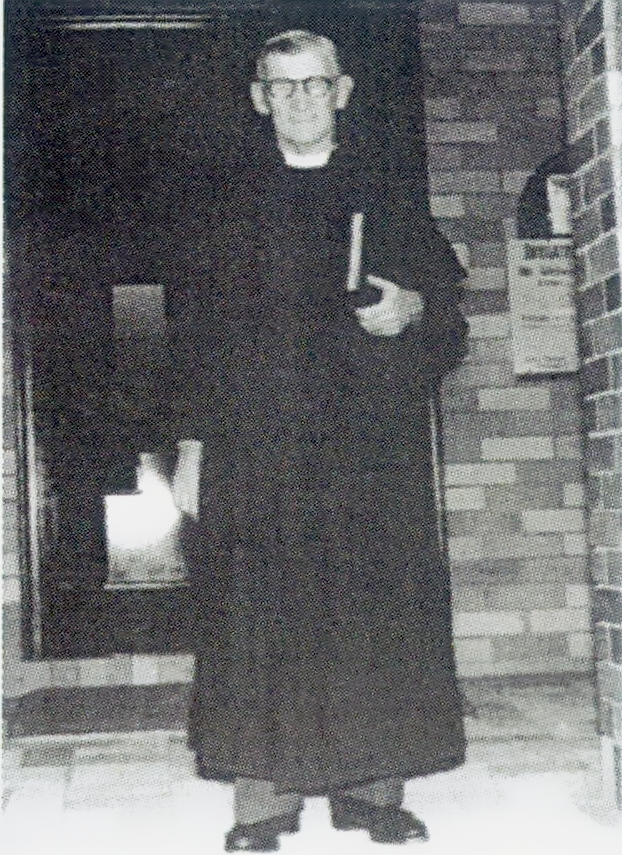
\includegraphics[width=1.\linewidth,center]{../images/EHSmith.png}
\caption{Rev E H Smith}
\end{center}
\end{figure}


Excerpts from Mrs Alison Coomber's book on the life of her father, titled `A GREAT BLOKE: The Life of Ernest Henry Smith,'\footnote{\emph{A GREAT BLOKE: The Life of Ernest Henry Smith --} compiled by his daughter, Mrs Alison Coomber. (Used with permission)} gives a first-hand insight into conditions for clergy at that time. This book is an important resource for anyone interested in the conditions, trials and tribulations as well as the joy of service to God in Rural Queensland, and indeed Australia, in these early closer-settlement years.

In her Foreword, Mrs Coomber gives an insight into the man himself. `\ldots he was \ldots{} kind, intelligent, loving, fun, not judgmental and very slow to anger \ldots{} always very quick to see and appreciate the inherent good in people.' He appears to be the perfect example of not just a Great Bloke but a Great Priest as well, even though, `many years ago, my father was described to me as `a great bloke, but a bit long-winded.'

In 1926 it was announced in the Diocesan periodical \emph{Church Chronicle} that he had been appointed on promotion, as Vicar of Murgon with the parish described as being a relatively new one, large in area but small in population. Murgon could hardly have been more different from bustling Maryborough. One redeeming factor was that his wife, Molly, had been a pupil-teacher there in 1916 and was familiar with the area.

`As well as the main church at Murgon, there were six smaller congregations at Boonara, Wondai, Goomeri, Kilkivan, Mondure and Tingoora with five even smaller dependencies for Ernie to administer to \ldots{} Abbeywood, Fat Hen Creek, Cinnabar, Proston and Barambah Settlement (later named Cherbourg) thus 12 in total. So, the Parish of Murgon in those days was a real test of endurance and strength for its Vicar, whose stipend was more than a Curate's but less than a Priest's\ldots{} When they first arrived at Murgon, they had no stipend for three months, and must have been living literally hand-to-mouth. Not an easy task for a pair of newly-weds.' Letters held in the Diocesan Archives in Brisbane, confirm (rather curtly at times) that the decision made by Wardens of the area in 1914 to advance monies on an end-of-quarter basis was not in accordance with Diocesan wishes but was most firmly and determinedly adhered to by the locals and was still in effect, Parish-wide over 10 years later.\footnote{\emph{A Tapestry in Faith --} St David's, Boonara, Centenary, 2014} The Smiths were also in grief following the stillbirth of their first child, Beth.

Added to these stresses, the area was feeling the effects of the depression following World War I. Funds were short in all areas and support of the church suffered the consequences as well. However, with his characteristic enthusiasm Ernie threw himself into his duties. The test of endurance is obvious as services register covering his first weeks in the parish confirm that he managed to travel to every one of the twelve centres at least once.

Murgon 1926: 10 January service register states: `No Service. Vicar ill.\emph{'} 13 January: `Induction as Vicar, Officiant the Rural Dean (J E\emph{)}\footnote{Diocesan Archives -- Murgon Parish Minutes -- DJ Box3}\emph{-} Rev Joseph Elliott who was rector of Maryborough at the time.

`\ldots eight lines written in Ernie's neat handwriting record the Easter meeting on 23 April 1926, a few months after he began work there. There were six people in attendance, not exactly a large gathering. Besides the Vicar were the Vicars Warden and the Peoples Warden, the Parish Treasurer and two others.' Page 40 identifies the two Wardens as being the same two faithful parishioners - Mr J S Mills as People's Warden and Mr S Trudgion as Vicar's Warden. The Treasurer is not identified.

The financial position appears to have been a matter of ongoing concern with the necessity to `raise funds by various means. The Women's Guild frequently `\ldots came to the rescue\ldots' Mrs Coomber

continues from the minutes, that the only business dealt with was the discussion and adoption of the balance sheet, and the Women's Guild was thanked for their contribution of \pounds450 to meet the building fund debt.

Guild assistance was called upon several more times over the next couple of years. Fund raising ventures included canvassing the district for contributions to organizing and holding a children's Ball in an effort to meet the diocesan assessment quota and to reduce the bank overdraft to under \pounds100.

Obviously, there continued to be a very active group of women in the Parish, lending generous support -- a mark of merit which can be attributed to such Guilds in all parishes.

An active Sunday School is mentioned, which also contributed financially as it `paid for the repairs to the lighting plant amounting to one pound ten shillings,' as electricity from the grid was obviously not yet connected to that fairly isolated area. (P40)

The 1927 Easter Meeting outlined the achievements of the parish. All who had contributed to the life of the parish were thanked, especially those who collected, organized functions, and taught at Sunday School. Special mention was given to the Women's Guild who had provided new hangings and kneelers.

The Services Register 1928 records the Easter 1 service at Murgon as Holy Communion with 13 communicants. On Friday 20 April at 8.00 pm, `4 boys and 9 females' were confirmed by Archbishop Gerald Sharp.\footnote{Diocese of Brisbane -- Murgon Services Register -- DJ 3, Box 2}

`Ernie's time at Murgon was coming to an end with a promotion in the wind.' The parish of Christ Church, Childers, offered Rev Smith the position of Rector, which was a promotion from his previous role of Vicar and carried an appropriate increase in salary.

A letter from the Archbishop to the Childers parish, dated 11 April 1928 advised that Rev Smith had accepted the position and was resigning Murgon as from 30 April. He had performed well in a situation that was far from easy and had impressed the Church hierarchy.\footnote{Murgon Parish Correspondence -- ACSQ -- Archives.}
\balance

\printendnotes[custom]
\setcounter{endnote}{0}
\chapter{1928--1932 : Rev Eric D Eglinton}
\nobalance

Vicar Eglinton was appointed to the Parochial District of Murgon soon after Rev Smith's departure, as an article in the 18 May 1928 Brisbane \emph{Courier,} headed `Welcome' indicates:

`A large number of people gathered in the School of Arts to welcome the Rev Eglinton, who has been appointed to take the place of Rev E H Smith, Church of England minister, transferred to Childers. Rev Eglinton was welcomed by Mr E H Standen and Rev T H Taylor (Methodist) after which a short musical programme was gone through. Songs were tendered by Missies E Duffie and R Bordiert, recitation by P Caswell and Hymn solos by Miss F Scurr and Mr J Trudgion, Cornet solo by Mr Keating and selections by the Murgon Orchestra. After the programme had been concluded dancing was indulged in. Music was supplied by the Murgon Orchestra and extras by D Anderson and Miss S Cole. The ladies provided supper.'\footnote{\emph{Brisbane Courier}, 18 May 1928.}

On arrival Vicar Eglinton was confronted with an Ecclesiastical Parish constituted of the Lands Department Parishes of Cloyna, Nangur, Mount McEwen, Cherbourg, Murgon, Charlestown, Johnstown, Barambah, Kadarga, Gallangowan, Manumbar, Kilkivan, Widgee, Brooyar, Goomeribong, Proston, Mondure, Boonara and Cushnie, From this extensive geographical area twelve centres of worship were operating -- six major centres with the capacity of the church buildings, were listed as being Murgon (100), Boonara (80), Wondai (80), Goomeri (100), Kilkivan (100) and Mondure (100) with another six outlying areas comprising Tingoora (60), plus, with no actual church buildings - Abbeywood, Fat Hen Creek, Cinnabar, Proston and Barambah Settlement.\footnote{\emph{Year Book --} 1919 -- 1927.}

Early in his ministry, other serious issues also had to be borne in mind. In 1927/28 the Bundaberg area, only a couple of hours north of Murgon, was hit by a devastating outbreak of Diphtheria. Many young lives were lost as a consequence. This resulted in the swabbing of the throats of 35 students at Murgon State Rural School following diagnosis of cases in the town. In view of the way events had unfolded in Bundaberg, it is easy to understand why such proactive measures were taken locally. On a lighter note, the paper also reported on the well-attended annual Church of England fundraising Ball, commenting that it `considerably augmented' church funds. Novelty dances were won by Miss Franks and Mr McLucas and Mr T Osbourne and partner. \footnote{\emph{Brisbane Courier,} 7 June 1928\emph{.}}

To facilitate smooth management and for parish council purposes, centre wardens were appointed namely: S Trudgian and D L Jones (Murgon), J Stanton (Boonara), R Borton and C Robertson (Wondai),C M Wimberley and H R Stanton (Goomeri), C W Waldock and H Zahnleiter (Kilkivan), T Roseby (Mondure), C Tesch and ? Northcott (Tingoora).\footnote{Diocesan Archives -- Murgon Parish Minutes -- DJ 3, Box 3.}

This period from 1928 to 1932 was a difficult one for this enormous parish and for its vicar. Demand for ministry increased incrementally as the extensive grazing properties gave way to smaller agriculture and dairy farming ventures and thus a rapid increase in population due to closer settlement. The established routine of two Holy Communion services and two Evensong gatherings continued. Congregations were substantial as 23 Communicants at Mondure, on 3 June (Trinity Sunday), 30 Communicants at Kilkivan on 10 June, Trinity 1, and 39 Communicants in Murgon on 17 June, Trinity 3, indicate. The vagaries of the weather continued to interfere with smooth running and regular congregations as seven consecutive low-attendance services in 1928 carried the side note ``Wet\emph{''.}\footnote{Diocesan Archives -- Murgon Parish Minutes -- DJ 3, Box 3.}

From 1914 to 1928, ministers continued to be plagued by difficulties with distances travelled and road conditions. Vehicles often became bogged after even small falls of rain and it was not uncommon at these times, and for other travel related reasons, for services to be cancelled. Rev Eglinton is reported to have had the dubious privilege of a Baby Austin as his mode of transport -- a very small car and a most unsuitable vehicle prone to breakdowns and tyre trouble resulting from the existing road conditions. He was often running late for services and on one occasion the Kilkivan service register shows that he spent two hours bogged in Wide Bay Creek before the ever-reliable old type of \emph{horse}power was used to drag the vehicle out.\footnote{St Mathew's Kilkivan \emph{Centenary Booklet} p. 6; This is confirmed by an entry in \emph{Glimpses Through the Years --} a centenary booklet produced for Goomeri's centenary celebrations in 2016.}




\begin{figure*}[!htb]
\begin{center}
\includegraphics[width=1.\textwidth,center]{../images/austin7.png}
\caption{Austin 7}
\end{center}
\end{figure*}


Several different ventures regarding clergy placement and parish boundaries were put forward for consideration. It is interesting to note that even with the aforementioned `tyranny of distance' between centres, the large number of worship places had remained in place until this time.\footnote{\emph{Glimpses Through the Years --} a centenary booklet produced for Goomeri's centenary.}

Changes were on the horizon, the first of such moves are recorded in the minutes of the Kilkivan Parish Council meeting held 17 December 1928. Mr C Waldock proposed a motion, seconded by Mr McKell, `that Mr D L Jones be Peoples Warden'. Mr Galloway was elected Auditor on a motion proposed by C A Wimberley, seconded by H P Stanton. Council members to be Ex-Officio members plus Messers T Wise, McKell, A White. F Peters, T D Kelley, T H Spencer, Stanley Maudsley, G Hughes, Wimberley, Middleborough, J E Stanton.

The final item mentioned is one of great significance showing that as early as 1928 moves were afoot to re-align parish boundaries. Mr D L Jones moved, seconded by J E Stanton, `that Mr C M Lloyd, D Jones, T M Wise, C Wimberley, G Hughes and Mr Galloway be representatives to meet in the matter of distance of parishes.'

Just one year after Rev Eglinton's arrival in Murgon, the 25 June 1928 service register entry records a visit by `Bishop Gerald, Brisbane' who officiated at the 7.30 pm Evensong in Goomeri. No doubt the current position and possible ways forward were discussed with the locals.

Diocesan documentation dated 31 October 1928 advises that the Archdeacon (Canon Garland) had submitted a report recommending that Murgon parish be subdivided into two Parochial Districts namely Murgon and Kilkivan. The Murgon district comprised the following places: Murgon, Wondai, Mondure, Tingoora, Proston, Abbeywood, Boat Mountain, Barambah Settlement, Hivesville and Cloyna and the Kilkivan district included Kilkivan, Goomeri, Boonara, Manumbar, Woolooga, Fat Hen Creek, Sexton and Cinnabar.

On the motion of Canon Garland, it was recommended that these two new Districts be formed. The document is signed: `Gerald, Brisbane' - and dated 2 August 1928.\footnote{Diocesan Archives -- Murgon Parish correspondence -ACSQ - signed +\emph{Gerald, Brisbane} and dated 31 October 1928.}

Rapidly increasing density of population in the Murgon district was undoubtedly the driving force behind the constitution of the two districts which operated separately and were known locally as Parish of Kilkivan and Parish of Murgon respectively.\footnote{JE Murphy and EW Easton, \emph{Wilderness to Wealth: being a history of the shires of Nanango, Kingaroy, Wondai, Murgon, Kilkivan and the Upper Yarraman portion of the Rosalie Shire, 1850-1950}, Brisbane, WR Smith \& Patterson, 1950, repr. 1974, p. 314.} While the problems with travel between the wide-spread centres within the parish continued, it seems also that financial constraints endured in the difficult years following World War I were still evident in this period and splitting the area into two zones could go a long way to alleviating this financial strain.

Rev Eglinton relocated to Goomeri with oversight of the Kilkivan district until 1932 thereby beginning a long association with Kilkivan, Goomeri and Boonara churches and the outlying regions of Fat Hen Creek. Sexton, Cinnabar and Woolooga. However, as mentioned in Chapter 3, services in some of these ceased soon after this though determined and enthusiastic moves for the construction of places of worship in Woolooga were made but sadly were discontinued after three years, financial issues having intervened. Rev Eglinton is credited with having initiated (though unsuccessful) moves towards having Woolooga and Sexton transferred to Gympie region. St Matthew's, Kilkivan, (established in 1888) had been serviced under the Tiaro umbrella until 1920.

Rev Eglinton and his wife were an active team in ministry and all church affairs. Mrs Eglinton worked tirelessly in running Ladies Guilds in Goomeri, Kilkivan and Boonara. Minutes attest to her serving as founding President at Boonara and Goomeri. As usual, these guilds were stalwarts in raising funds through time honoured activities such as catering, hosting social functions, fetes, garden parties and street stalls as well as helping organise concerts and balls.\footnote{\emph{Diocesan Archives -} Murgon Parish Minutes -- \emph{Holy Trinity,} Windera\emph{,} Guild Minutes p. 1 - DJ 3, Box 3.}
\balance

\printendnotes[custom]
\setcounter{endnote}{0}
\chapter{1929--1933 : Rev Howard Saull}
\nobalance

With Rev Eglinton separately installed in Goomeri, Rev Saull began as Vicar of the Murgon portion of the newly-divided former parochial district. Although his induction service was conducted by Rev William Powning Glover (Archdeacon, Toowoomba, 1927-1945) on 4 February, his ministry began the morning after his arrival in the parish. Vicar Saull conducted his first service in Murgon at 7.30 am on Wednesday, 2 January 1929 -- attendance 3. However, the congregation increased to 15 communicants the following Sunday at the 7.30 am service, followed by the 11.00 am Eucharist at St Mary's, Wondai -- communicants 3. His day continued with two more Evensong services -- 2.30 pm at St George's, Tingoora and 7.30 pm in Murgon. This busy routine continued throughout January though varied as regards venues to accommodate the many outlying centres -- usually with a service of Evensong, although the 13 January register mentions Holy Communion at St Faith's, Mondure with a congregation of 15.

The month of February appears to have been a difficult one for the new vicar as several notes in the service register indicate -- for example, `No Service -- Raining'; `Heavy storm'; `Roads impassable'\emph{.} Such comments provide us with a clear picture of the `tyrannies' not only of distance but also of weather and the impact such natural events made on the rough and unsealed roads to be travelled. A Mr H Legatt was installed as a Lay Reader for Christ Church Murgon on 1 July 1929, an appointment no doubt gladly welcomed by Rev Saull.\footnote{Diocesan Archives -- Murgon Parish Services Register 1927 -- 1937 -- DJ 3, Box2}

Although the constant need to raise funds continued during these between-the-wars years, there were many happy times associated with church activities. As usual, the Guild ladies were at the fore with great assistance given by their menfolk, congregation members and local businesses.

On 23 December,1929 the \emph{Courier Mail} lists such an event:

Murgon: \emph{Christmas Tree \textbf{-- }}A Christmas Tree under the auspices of the local Church of England, was held in the School of Arts on Friday night last, there being a good attendance. The children received gifts from the tree, and dancing was indulged in by the older folk. The music for the evening was supplied by Miss Perrett's orchestra. \footnote{\emph{Courier Mail,} Brisbane, 29 December 1929}

A \emph{Courier Mail} article dated 3 November 1930 another such event, providing enjoyable social engagement for young and not so young, alike. `A fancy-dress children's ball\emph{\textbf{,}} organised by the ladies of the Church of England, was held in the Star Theatre, Murgon last week. Mr J Tiernan was in charge of the programme, whilst Mr C Hansen supervised the grand march. Novelty dances were won by Misses I Houghton, V Dow and B Tiernan, and competitions by Mr S Fenner and Misses Hold and Beitzel. A Maypole dance and folk dancing items were given by a number of children'. A 1931, 14 September edition of the same newspaper notes the 4 September official opening of Murgon's new Rifle Range by the club president and chairman of the Murgon Shire Council, Mr A Leich which had been assisted with finance by a grant from the Defence Department\emph{.}\footnote{\emph{Courier Mail,} Brisbane, 30 November 1930 and 14 September 1931, p 8}

Two articles with reference to the church at Hivesville appeared in the \emph{Church Chronicle} during 1932. The first in the 1 July edition featured an article on the official opening of the Church of the Holy Spirit by Rev H Saull on 15 May 1932 and included a photo of the church and congregation. A small article followed which is printed in full in the separate section on the church later in this book. The second appeared in the 1 November edition's article from Murgon Parish. This also appears in the Hivesville Church section.\footnote{\emph{The Church Chronicle,}1 July 1932, p. 217; and 1 November 1932, p 363}

September 1932 services register reveal a very full two-day visit by from Bishop Horace Henry Dixon. The entry for 11.00 am on Saturday, 10 September stated `Consecration of Mondure Cemetery'\emph{.} This had been a long-established burial place dating from early settlement times, St Faith's Church having later been built adjacent. Later at 3.00 pm Bishop Dixon officiated at a service of Confirmation in Murgon for 10 girls and 9 boys.

Sunday 11 September saw the Bishop officiating and preaching at 7.30 am Holy Communion in Murgon followed by a drive to Wondai for 10.00 am Holy Communion service. His busy day continued with travel to Hivesville where, at 1.30 pm, the Church of the Holy Spirit was blessed and dedicated along with the confirmation of seven boys and eight girls. This was followed by the private Confirmation of two girls at Cushnie and by 1.30 pm he was back to conduct Evensong in Murgon.\footnote{Diocesan Archives -- Murgon Parish Services Register, 1927 -- 1937 -- DJ 3, Box 2}

The last entry in Rev Saull's handwriting for 26 February 1933 stated blandly -- ``\emph{No Service Vicar ill''.} It appears a period of illness follows as the next entry was simply dated March and was listed as 7.30 pm, Evensong, Murgon and signed `DGL'. Church records confirm that David George Tweedy and H Leggat were both registered Lay Readers in the parish who contributed by conducting services as required on an irregular basis. There are no entries after this date for Rev Saull in the Murgon Services Register or the Kilkivan Services Register.

After the initial optimism leading to two separation into two zones, financial constraints appear to have been the main contributing factor leading to the collapse of the `two districts' scheme and also to Rev Saull's decline in health. Rev Saull relocated to St Luke's, Rosewood, some three months later, commencing duties as acting Rector on 1 June,1933. His first service in that parish is noted as being 4 June 1934.

During this 1928-1933 period, while ministry matters remained relatively stable, there were many undercurrents of discontent regarding parish boundaries and a great deal of parochialism evident between the centres.

\emph{Glimpses Through the Years} indicates the indefatigable Archdeacon Glover seems to have worked tirelessly to provide a solution acceptable to all parties -- a very difficult task indeed! However, despite the best efforts of the two vicars, parish councillors and guilds, the venture `proved to be financially unviable.'\footnote{\emph{Glimpses Through the Years --} Goomeri Centenary Booklet, p. 5} Building on the 1928 proposals put forward by Canon Garland and signed into effect by Archbishop Sharp in August of that year, (as mentioned above) re division of areas, Glover chaired a meeting in Goomeri on 16 September 1930 where his account of meeting with representatives in Murgon indicated they were `not in favour of amalgamating with Kilkivan Parish.'

Through the 1930/1933 period Archdeacon Glover worked tirelessly, conducting many meetings and consultations with all parties in an effort to provide a solution in a resistant atmosphere. It appears that `the ever-patient Archdeacon Glover' had to contend, not only with a resistant attitude from the Murgon end, but also similar negativity for Kilkivan who stood \emph{`}firm in its resistance to becoming a part of' a Murgon Parish.

Finally, to all appearances, pressure to bring the matter to a head brought results. A lecture headed `Glimpses of the Past. A lecture on the early history of the Anglican Church in the Wide Bay and Burnett Archdeaconry given at the Pialba Clergy Conference in April 1971 by the Venerable H J Richards, BA, Th L. stated that: On 18 February 1933 Archdeacon Glover chaired a meeting in Goomeri where Mr David L Jones moved (seconded by Mr Wimberley) ``that it be an \textbf{instruction} to the parish representatives at the meeting with the (Diocesan) Committee in Brisbane \textbf{to agree to} the Parish of Kilkivan taking over part of the Parish of Murgon Viz. the township of Murgon plus Windera and also Booubyjan, from the Parish of Gayndah; the parish to take over half the debt of \pounds300 owing by the Parish of Nanango but accept no liability in regard to the debt of \pounds400 in the Murgon church. Carried.''\,'\footnote{\emph{Glimpses of the Past.} A lecture on the early history of the Anglican Church in the wide Bay and Burnett Archdeaconry given at the Pialba Clergy Conference in April 1971 by the Venerable HJ Richards, BA, Th L.}

Thus, the Parochial District of Kilkivan was re constituted (to include Murgon) with Wondai as a separate district. The only deviation from this proposal appears to have been that objections were raised by the interested parties regarding Booubyjan/Gayndah and it was agreed that the current arrangements would remain.
\balance

\printendnotes[custom]
\setcounter{endnote}{0}
\chapter{1932--1942 : Rev James Lee-Warner}
\nobalance

Rev James Lee-Warner (1889 -- 1975) followed Rev Eric Eglinton as Vicar of the newly proclaimed Parochial district of Kilkivan on 22 May 1932 and continued to reside in Goomeri. Although, `officially proclaimed' as a total parish entity, it continued to function as two districts until 1933.

The new vicar had a very varied ministry story prior to his appointment to this parish. He began his clerical career in 1913 with three years as curate at Rythope, Durham, England, before serving as a soldier (though a deacon) 1915-1919 then returning to ordained ministry. His ministry took him all over the world, in many roles, including being custodian, Department of Antiquities, Palestine. He eventually arrived in Australia in 1926, where he served in Warwick, South Brisbane, Dalby and Chinchilla, then as a missionary chaplain to the Brisbane Diocese before finally taking up his appointment as `Vicar - Parish of Kilkivan' which, at that time, covered Windera and Boonara as well as Kilkivan and Goomeri and the smaller satellite centres. There was some overlapping in bringing the new Parish of Kilkivan into full function as Rev Saull continued to serve as Vicar of the Murgon until June 1933.

Parochial bias and hard-line attitudes confronted Rev Lee-Warner from the time of his arrival. According to the Kilkivan church's services register, his first service there was on 22 May 1932. The Kilkivan Centenary booklet states: `Kilkivan parishioners always seem to have favoured Low Church practice, and in fact, Rev Lee Warner was warned by the Parish Wardens on his arrival to `dispense with the High Church doctrines of the Parish.'\footnote{St Matthew's Kilkivan Centenary Booklet p. 9}

From the Kilkivan services register -- 22 May 1932: `The Rev James Lee-Warner Th. A. was this day licenced as Vicar of the Church and Parochial district of St Matthew's, Kilkivan and appointed to reside within the said district.'\footnote{Diocese of Brisbane, Murgon Services Register -- DJ 3, Box 2} Murgon welcomed him with a pleasant gathering in the Oddfellows Hall.

An article from a 1933 \emph{The Church Chronicle} contains the Service List from March 5 to April 2 and indicates a busy schedule of four or five services every Sunday and good coverage of the large and well-spread Murgon Parish and further records:

\emph{`The Christmas efforts were not so successful as two years ago, only \pounds30 being made from the whole parish, but there is a fair amount of toys left in hand. Rain spoilt the Windera Christmas Tree, and Wondai decided not to have one. Hivesville was the most successful, being followed by Murgon, Proston and Tingoora. Christmas Day was easily a record, the number of communicants in Murgon being a record for any service held in the parish since the present book started in 1919, the date of separation from Nanango. This equally applies to the other services held on Christmas Day. Lent starts on Wednesday, 1 March. There will be a special service and address in Murgon every Wednesday night. May I remind you that the 40 days of Lent are ``days of fasting, or abstinence''.'}\footnote{\emph{The Church Chronicle}- March 1, 1933, p.93.}

Rev Lee-Warner's first entry for a service in Murgon was for Wednesday 9 March 1933 and is listed as Lent Service and Address\emph{,} followed by a 7.00 am HC Thursday 10 March.

The rest of March followed an intriguing pattern of Sunday Evensongs conducted by \emph{DGT --} Lay Reader, David George Tweedy who was licenced as a lay reader for Christ Church Murgon until 2 September 1941. Regular, Lee-Warner-led week-day services of Morning Prayer and address on Wednesdays and Holy Communion at times varying over 6.30 am, 7.00 am, 7.30 am on Thursday or Friday, continued for the remainder of March. There is no mention of any visits to outlying centres in the Murgon district. This would seem to confirm the general assumption that Rev Saull was ill at the time, possibly on leave, so only such entries were in the Murgon Services Register while Rev Eglinton would have maintained the former Parish Register for his area in Goomeri. Sadly, this register has been lost to posterity. There is a similar gap from September 1932 until 1944 in the Boonara Services Register. However, anecdotal evidence indicates Rev Lee-Warner's diligence in providing services and a willingness to co-operate with both sections of the parish, still divided, at least by attitude, though officially `one'. Rev Lee-Warner and Mr Tweedy conducted Murgon service until 27 August, after which Lee-Warner undertook all services.

Rev E H Smith returned to officiate at three services in March 1935. Other priests who undertook services on a periodic basis up to 1937 include H V Golding and J E Devine. Side notes carefully entered in the register of services provides an historical record of the era. Lee-Warner's entry in the Memoranda column marked the passing of King George V with service on Tuesday 28 January 1936 at 6.30 am - a Requiem and Eucharist attended by fifteen persons. During the month of February, Sunday services plus one on Ash Wednesday service were confined to Murgon. However, the 1 March Lent 1 service was at Boonara at 11.00 am. Further side notes include -- Collection 1/3d ABM; Refreshment Sunday; and one marked `Temperance'.\footnote{Diocese of Brisbane, Murgon Services Register -- DJ 3, Box 2}

Though named Parish of Kilkivan as a recognition of Kilkivan's historical significance in the early settlement era, the administration centre and residence were both located in Murgon, in an attempt to satisfy and acknowledge the two main centres. Rev Lee Warner expressed his opinion that the rectory needed to be in Murgon rather than Goomeri `because of Cherbourg'.

The Pimlott's cottage in Taylor Street became available for purchase. It was generously offered to the parish by Mr and Mrs Pimlott at a cost of \pounds200 on a deposit of \pounds50 to be paid off, interest free, over 10 years. A reference was made to the possibility of monies `from the Shepherd Bequest' being utilized in making the dwelling `ready for the rector to move into'. However Diocesan advice was that this was not possible. The attitude of parochial non-cooperation again appeared with Kilkivan representatives stating that they were `of the opinion that Murgon was not yet part of the parish' but adding that they would `have no objections to renting the house if the Murgon bought it' themselves.\footnote{Diocesan Correspondence files, October 1935, Diocesan Records and Archives Centre, Brisbane}

Archdeacon Glover again intervened. His considered opinion was that the house, `centrally located and conveniently placed as regards the church', was cheap at the offered price of \pounds200 (as it had been valued at \pounds350). However, in his 29 November 1935 letter\footnote{Diocesan Correspondence file, 29 November 1935, Diocesan Records and Archives Centre, Brisbane}, he observed that responsibility for raising the funds rests entirely with Murgon which already owes \pounds400 on its current account and has committed to \pounds50/pa to the parish's working account. With `no money in hand' the full purchase price would need to be borrowed and `they should have a definite amount of money in hand' before incurring more debt.

Archdeacon Glover noted that `Murgon and Kilkivan regard themselves independent units' whereas Murgon is definitely now part of Kilkivan Parish and that `This point to be made clear to both sections of the Parish'. He also conceded that `As to the future, no undertaking could be given at the present time as to whether Murgon should remain in Kilkivan Parish or whether it should become part of proposed Wondai district.'




\begin{figure}
\begin{center}
\includegraphics[width=1.\linewidth,center]{../images/reportMurgonHouse.png}
\caption{Report Murgon House}
\end{center}
\end{figure}


Letters to Bishop Dixon and the Diocesan Property and Finance Board, signed by G Waldock and P Sing, indicated that the Murgon centre had pressed ahead and the house had been purchased, the rector was now installed, and that rental by the parish was set at 15 shillings per week. The necessary paperwork re transferring of deeds etc was being completed.\footnote{Diocesan Correspondence files, November 1935 to February 1936, Diocesan Records and Archives Centre, Brisbane}

A 1936 \emph{South Burnett Times} article documents a change of residency from Goomeri to Murgon. It states: `The location of the Minister in charge of the Murgon Parish of the Church of England has again reverted to Murgon, and Rev Lee-Warner, after several years' residence in Goomeri, last week moved to Murgon where he will in future reside. No Church of England minister has been stationed in Murgon since the departure of Rev H Saull some years ago.'\footnote{The \emph{South Burnett Times,} 21 February 1936. Newspaper cutting contributed by Jeff and Muriel Schultz.}

While it appears that the Murgon centre was desirous of upgrading the interior furniture as on 24 September 1936, the Diocesan Records and Archives Centre recorded: `A faculty was this day issued authorising the erection in the Church of Christ Church Murgon of an altar of Silky Oak with Cross in centre and Credence Table -- no objection having been raised' other evidence indicates that these items were there when the church was dedicated in April 1920 and the oversight was simply being rectified some 16 years later.\footnote{Diocesan Records and Archives Centre, Brisbane.}

Rev Lee-Warner contributed to the Jubilee Booklet of St Matthew's church, Kilkivan in 1938, mentioning a reference to Kilkivan area in Bush Notes when the Bush Brothers operated out of Gayndah. The booklet (p. 15) also states that Lee-Warner `wrote a very good history of the church at that time -- priced at One Shilling -- \ldots affectionally known as The Little Red Book'. It remains a valued historical record of the period immediately preceding the 1939 outbreak of the second world war which was to have a significant impact on the local church. Rev Steer returned to the area for that special day at Kilkivan, preaching at an 11.00 am service and at evensong. Between services, the worshippers partook of a Basket Picnic in the Kilkivan church grounds.

World War II had a significant impact on the district. There were several known rifle ranges in the parish and stories of the presence of soldiers crossing fields where dairy cattle were grazing are common in the area. The presence of these soldiers resulted in surge of social activities and church involvement. Rifle Clubs were first formed in the area in the very early 1900s, but an understandable resurgence occurred during this period -- often with mixed-gender membership.

An entry in the cash book of the Murgon Church of England Ladies Guild, 13 August 1940 records a donation of \pounds1 to Soldiers and Sailors Help Society and 24 October 1940, the purchase of an Airman Doll plus postage -- possibly for use as a raffle prize. However, it must have proved to be unsuitable for purposes as the next page shows a cash refund for `Airman Doll'.\footnote{Murgon Church of England Ladies Guild Cash Book 1940-1966} It was around this time that the names of May and Bill Gedge began to appear regularly in church documentation.

A newspaper clipping dated 17 October 1943 speaks of an entertainment and fundraising venture `with a difference' in Murgon. `A bridge party, in aid of the funds of the local Church of England, was held at the residence of Mr and Mrs F R Skyring. The bridge prizes were won by Mr V G Tickle and Mrs N Kidd. Competitions were won by Mrs Tickle and Mrs Roberts.' This article contains names significant in Murgon church's history. Tickle was a pharmacist, Skyring is mentioned in early minutes and Roberts family still have descendants operating a solicitors' office and taxation service in Murgon.~ Bill Roberts (recently deceased and son of GW Roberts the first solicitor and taxation agent in Murgon) was Shire Council Chairman for many years and a valued contributor to the Anglican church.~ His wife Mary (nee Cobb) was the daughter of early settler settlers.~ Cobbs Hill, near Cloyna, is named after them.\footnote{Newspaper clipping -- Courtesy Jeff and Muriel Schultz, Murgon.}

Several points indicate that Rev Lee Warner carried an affection for Goomeri - his initial place of residence in the parish. He is credited locally with having brought Olive and Pomegranate seeds from the Holy Land which he successfully managed to cultivate. The resulting Olive tree still grows happily at the rear of the Church of the Epiphany while the Pomegranate bush stood until around the year 2000 when termite infestation of its root system, posing a danger to the church building, necessitated its removal.\footnote{\emph{Glimpses Through the Years --} Goomeri Centenary Booklet, p. 18.}

Mrs Sylvia Jennings visited the parish in October 1995. As Rev Lee Warner's daughter, she had decided to make a `nostalgia tour' of the parish which held both fond and sad memories for her. She was pleased to see the two trees still growing, the Pomegranate carrying fruit at the time. Her mother Elizabeth's death had been commemorated by a framed print under glass -- \emph{In the Glory of God --} organized in honour of her efforts as a Sunday School teacher there, the plaque reading `In Memory of Elizabeth Lee Warner. Died 04-09-1956. Given by the Pupils and Staff of the Church of the Epiphany Sunday School, 21-07-1957.` A letter to the Goomeri Guild in August 1995 requested a service to dedicate a donated Ciborium for Goomeri Church donated by Mrs Jennings was the prompt for her whole of parish visit. Gifted in memory of her father and honouring his time there as vicar and purchased from Pelligrine (Brisbane) for \$245 with an extra \$80 for engraving and re-silvering over the engraving, the beautiful Ciborium was officially dedicated as requested in a `whole of parish' service by the rector, Fr Bavin Clarke, on 22 October 1995, appropriately, in the presence of his daughter Sylvia.\footnote{Goomeri Guild Notes -- Held by secretary in Goomeri.}

Rev Lee-Warner ministered to the parish as Vicar until 10 September 1940, leaving to take up his position as rector of the parish of Beaudesert on 14 September 1940. Lee-Warner's last service as recorded in the Murgon Services Register was held 8 September 1940.\footnote{St Matthew's Kilkivan, Centenary Booklet, P.5 and p.1} At the time of his leaving,

The Year Book records synodsmen as E D G Stanley and R Reugg, with Messrs Jeffries and Stanton as wardens.

Records indicate that wanderlust subsequently took him to North Africa (1963 -1965) where he served in H M Embassy. His final posting in his priestly career (1965 -- 1667) was as Chaplain at All Saints Marseilles -- Gibraltar. He passed away in 1975. He and his wife, Margaret Elizabeth (Hewlett) were held in high regard by all the congregations he served.\footnote{Diocesan Clergy Records, Diocesan Archives Centre, Brisbane}
\balance

\printendnotes[custom]
\setcounter{endnote}{0}
\chapter{1940--1944 : Rev Harold Wilmot Griffiths}
\nobalance

Rev HW Griffiths (1892 -- 1951) was ordained in 1927 prior to arriving in Australia where, on 21 December 1934 he took up a position as priest-in-charge at Miriam Vale, diocese of Rockhampton, later moving to Blackall where he served as rector till 8 November 1940

By 1940 World War II was raging and having a great effect on the Australian population. Rev Griffiths' three and a half year stay in the parish commenced on 24 November. 26 parishioners attended the Sunday before Advent 7.30 pm Holy Communion service in Murgon, no doubt with the war to the forefront of their prayers as many local young men and women were already involved in the forces. Christmas Day, Wednesday 25 December, hosted one only service of Holy Communion with 31 attendees with offerings totalling \pounds1-5-6.\footnote{Diocese of Brisbane -- Kilkivan Services Register -- DJ 3, Box 2} The 1940 Year Books names Kilkivan, Boonara, Goomeri, Murgon, Fat Hen Creek and Manumbar as places of worship, S Fenwick as synodsman with R B Jeffries and J S Stanton as wardens.




\begin{figure}
\begin{center}
\includegraphics[width=1.\linewidth,center]{../images/kilkivanServiceRegister.png}
\caption{Kilkivan Service Register 1937-51}
\end{center}
\end{figure}


During the early stages of World War II, The United States of America was officially neutral and thus precluded from participating in the conflicts in both Europe and Asia. US maintained an armed presence in the Pacific and was officially engaging in diplomatic negotiations with Japan for possible peace in Asia. However, the unannounced bombing of the USA base in Pearl Harbour on 7 December 1941 led to their declaration of war against Japan on 11 December 1941 and to Germany's subsequent declaration of war against the USA. These events impacted heavily on the local citizens, many of whom were of British, Irish, or other European ethnic origins.\footnote{Wikipedia}

With the advance of the Japanese army resembling an avalanche approaching our shores, a fall-back defence deployment known as the Brisbane Line was formed. Murgon was the designated headquarters of the 3\textsuperscript{rd} Armoured Division of 16,000 troops. Troops from many and varied Divisions and Squadrons were stationed throughout the whole Murgon area from Yarraman and Kingaroy to Manumbar, Gympie and Windera and all areas in between. \emph{Murgon in Focus} carries an account from `the official war diary (24 April 1943) (secret until 1973)' indicating the `location of the 3\textsuperscript{rd} Armoured Division \ldots{} positioning \ldots{} began on Christmas Day 1942'\footnote{Murgon In Focus (page 211)}

In Murgon 26 people were present for a 7.30 am Holy Communion service with Evensong at 7.30 pm the following Sunday, 1 December -- Advent 1, while on Advent 2, a single 7.30 pm Evensong service was celebrated. A special Children's service and a Memorial Thanksgiving service were subsequently celebrated with offerings of \pounds3-3-4, an amazing amount for the time and circumstances.\footnote{Diocese of Brisbane, Murgon Services Register -- DJ 3, Box 2}

All levels of society and all ages need the Lord more urgently in such times and these services would have helped bring the Peace of God to the hearts of parishioners. People still, today, speak of the privations endured during these war time years and the ones which followed with severe rationing of necessary and basic items such as fuel. This in no small way hindered the provision of regular church services in this large parish. Along with the shortage of manpower to run farms and industries, congregations were also faced with added difficulties of supply shortages regarding their means of church attendance.

People on the land fared better, on the whole, than those in the urban areas with regard to food supplies, particularly the dairy farmers. Vegetable gardens were a high priority in all areas and chickens were a common site even in smaller town allotments with some town dwellers even having the luxury of a house cow. Farmers had the added advantage of a more accessible meat supply with their cattle and piggeries though the slaughtering of same was an added chore. Bartering was common. The advent of railways to outlying areas proved a life-saving bonus to many. Generous residents, town and country, were very open-handed in helping others in need, and indeed, by showing appreciation for the efforts of their clergy. Many stories are told of `swaggies' traipsing the land in search of odd jobs often for payment in the form of a meal and of families reduced to living in tents on creek banks, living a hand to mouth existence with fish, rabbits etc and whatever else could be gleaned `off the land' augmented occasionally with hand-outs from the locals and the church. Times were very tough for many people.

The first service register entry for 1941 was Evensong on 5\textsuperscript{th} January. Ministry-wise, Murgon continued to be well provided for over the following period, with the outlying areas of Goomeri and Kilkivan covered adequately, considering the circumstances. Boonara and Windera seem to have been on a one-per-month visit from Rev Griffiths and Cherbourg church received attention mostly from Lay Reader, Mr W Atkins.

One service with a difference was held 2 March -- Lent 1 -- where the name of AC Flint, Organising

Secretary for ABM is listed as officiating. During 1941, various efforts were made to combine some much-needed social engagement with extra church funding. Several entries such as Social Afternoon, Fete Takings, Produce Stall, Raffle, Concert and Garden Party, to name but a few, in the Murgon Guild Cash book attest to this. Mrs Griffiths was very actively involved in these parish

activities, with her name appearing several times in regard to the receipt of funds raised by her.\footnote{Murgon Guild Cash Book -- March 1940 -- March 1966}

In 1942, with activities still greatly curtailed by petrol rationing, shortage of supplies and finance, Rev Griffiths `appealed for more direct giving as it was `extremely difficult to raise money with concerts etc in the sad days of war.' He also asked people in all centres to bring evacuees to Church and to be more hospitable to the troops stationed in the camps their area. On another occasion he suggested that the Church of England dairymen should seek advice from the Roman Catholic dairymen on how to get to Church on time for early church services as only the 11.00 am or later services were well attended.' \footnote{St Matthew's Kilkivan Centenary Booklet p. 11}

The Annual General Meeting held 17 May 1944 recorded an attendance of twelve, being regular representatives from each centre, along with six apologies. The vicar's report covered the past year's parish events and included thanks to all who had contributed and assisted him throughout. The meeting oversaw the appointment of a familiar list of office bearers for the following year (which included the appointment of Mr R Pearson as a parish council representative in place of his late father).

The secretary was asked to write to the Diocese regarding the non-receipt of grant monies to assist in servicing Cherbourg Settlement which was provided with church services by the vicar and lay readers. A Sunday School operated weekly at a cost to the parish. Recompense was sought.

While the financial position was considered `not bad' it was felt `a special effort to be made by each centre to fulfil their quotas to keep the parish at a desirable level. Small finance committees at each centre was recommended to attain this end.' Quotas, with the exception of Fat Hen Creek, were unchanged. Murgon, Goomeri, Boonara and Kilkivan were asked to each contribute \pounds5 towards the liquidation of the Car Fund of \pounds20.

A letter of sympathy was to be sent to Mr Wimberley `expressing the council's deep concern over his illness and wishing him a speedy recovery.' and an invitation was issued by Murgon centre to other areas to attend Church of England Men's Society (CEMS) meetings held on the second Thursday of each month.

The meeting concluded in the usual way with welcome refreshments again provided by the willing band of Goomeri guild ladies who were thanked wholeheartedly.

In his article in the 1 January 1943 \emph{Church Chronicle}, Rev Griffiths wrote of the trials envisaged for the year ahead but assured readers that by `keeping touch with the Eternal Source of Strength' they with would be able to `face the unknown without fear'. \footnote{Church Chronicle -- 1 January 1943}

By 1943 the several camps for training soldiers in the area provided Padres assisting Rev Griffiths in ministry by actively participating in the provision of church services in the district and with soldiers under their care also attending. Two names mentioned are Padre Burnett and Padre McCulloch. For example, on 15 January six services were held in the parish. Padre Stewart Burnett officiated at 7.30 am Holy Communion and again at 7.30 pm Evensong, both in Murgon. Also, at 7.30 pm, Lay Reader Mr W Atkins (commonly referred to as Bill or Willie) held an Evensong service at Cherbourg Settlement (CAS). In between these hours, Rev Griffiths was busy further afield with 11.00 am Holy Communion, Goomeri; Windera - 3.00 pm Evensong; then back for a second service in Goomeri at 7.30 pm also Evensong. With this arrangement, Murgon and Cherbourg were well covered, so a similar basic pattern of services continued almost unchanged through January and beyond, though weekly variations were made to Rev Griffiths' schedule to cater for all outlying church centres.

Several army camps in the Murgon, Goomeri and Kilkivan areas are recalled with locations also indicated on maps of the time. Notations in the Memoranda column made specific reference to the soldiers and the camps, some with arrows pointing to identify church services and the enhanced attendance figures.

One service in particular stands out: Sunday 25 April 1943, Easter Day, recorded an attendance of 110 in Murgon, Goomeri 36, and Kilkivan 37, at their respective morning Holy Communion services. This was followed on Monday 26 April with the towns of Murgon 9.00 am, and Goomeri 11.00 am, commemorating Anzac Day with parades and Memorial Services conducted by Rev Griffiths.

The \emph{Church Chronicle} of 1 January carried information from Kilkivan parish. After wishing all a happy new year, Rev Griffiths commented on the fact that for the past year the district had hosted thousands of service persons. He expressed his deep thankfulness for `the hospitality given them, and also the maintenance of decent living.' His article concluded with notice of suspended services of 9, 16 and 23 January with resumption on 30 January. During his leave, if needed, his services could be accessed via the wardens. Mr Downing consented to assist if necessary.\footnote{Church Chronicle -- 1 January 1944 p.26}

With the trials and tribulations which war had imposed on the parish above the usual ones of administration, travel and finance, the parish had come through in a relatively favourable state. The possibility of replacing the ageing and well-worn vehicle was under consideration. Diocesan correspondence supports the positive state of the parish with a letter from Rev Griffiths requesting consideration be given to raising the status from `Parochial District of Kilkivan' to `Parish' to provide impetus for further growth, suggesting further that acceptance of the proposal `\emph{by Easter'} would be very welcome. Minimum stipend at the time was \pounds310. This had been in place for the past three years and Rev Griffiths was happy for this to continue along with a parish-provided car allowance of \pounds100. A copy of a letter to Gayndah Parish, signed by R B Jeffries and J E Stanton (Wardens), requested that the Booubyjan centre be transferred to Kilkivan control as it was in `a better position to give regular services.'

One happy occasion arising from the presence of troops in the area was the marriage of local lass, Barbara Mary Wrigley, daughter of Walter and Mabel Wrigley, to Donald Bert Hanson, AIF, (Zeehan, Tasmania) on 12 February 1944, celebrated in Christ Church Murgon by Rev Griffiths with Miss Dobe at the organ. The bride was attended by Matron of Honour, Mrs A Aubrey, and bridesmaids, Missies Bonnie Burton and Peggy Fuller. Mr Vic Jordan (Longford, Tasmania) was best man and Mr W Crawford (Brisbane) was groomsman. An extensive account of the wedding was published in the local newspaper, giving detailed descriptions of frocking (including style and colour) of the bridal party including mother of the bride, as well as of the bouquets and floral arrangements in the church and at the reception.\footnote{South Burnett Times article -- newspaper clipping and photo -- Donna Hindley (nee Hanson)}




\begin{figure}
\begin{center}
\includegraphics[width=1.\linewidth,center]{../images/hansonWrigley.jpg}
\caption{Donald and Barbara Hanson (nee Wrigley)}
\end{center}
\end{figure}

The Parish Annual General Meeting was held in the Goomeri CWA rooms 30 April 1944 with Rev

Griffiths in the chair and the familiar names of Sing, Waldock, Atkins, Sempf, Zahnleiter, Jeffries, Stumm, R and DL Jones, J and H P Stanton, Tate, Beitzel and Wimberley attending. Bardrick and Pearson were apologies. After dealing with the matters of minutes, correspondence, reports and quotas, officer-bearers are listed as: J E Stanton -- Rectors Warden; R Jeffries -- Peoples Warden; H C Kemp -- Secretary / Treasurer; Synod representatives -- Messrs Stanley and Rewig.

A visit by the Archbishop in May was announced with confirmation services 15 May in Wondai; 16 May -- Murgon and Goomeri; 17 May -- Kilkivan. Arrangements were made for his welcome at the various centres with Messrs Waldock and Atkins to meet the Archbishop on his arrival in the parish.

Vicar Griffiths addressed the meeting, thanking members for such a good attendance and for all the assistance, fellowship and personal support afforded him by the wardens, parish council members, ladies guilds and the thriving Sunday Schools, particularly in Murgon, Goomeri and Kilkivan. He then announced that this would be his last meeting with them, having accepted the Archbishop's invitation to move to the Parish of Palmwoods. Six members expressed the sincere regret of all the parishioners, stating that they `would miss him and the good work he was doing among the people.' They `wished him good health and every success and happiness in his new parish.'

Rev Griffiths' time in the Parish of Kilkivan drew to a close on 17 May1944. He moved to the parochial district of Palmwoods where he served till February 1947. Later positions included Beaudesert and Lutwyche. His years of ministry concluded with him holding a general licence in Brisbane until his death in 1974.\footnote{Diocesan Clergy Records, Diocesan Archives, Brisbane}
\balance

\printendnotes[custom]
\setcounter{endnote}{0}
\chapter{1944--1946 : Rev Alfred Stephen Jull}
\nobalance

In 1944 the parish had applied through its vicar Rev Griffiths to be granted benefice parish status. Diocesan Council received the request on 12 April 1944\footnote{Diocesan Council Minutes, 12 April 1944} and on 4 May adopted the `recommendation to raise the status to benefice with a rector.\footnote{Diocesan Council Minutes, 12 April 1944} Consequently, Rev Jull (1914-1982), after arriving in the parish on 1 July 1944, was officially inducted as Rector of the Parish of Kilkivan in a service in Murgon conducted by his Grace, Archbishop Reginald Halse on 31 July 1944. Other signatures accompanying Archbishop Reginald's include the Venerable Archdeacon Ernest Read Crittenden, C S P Blacklet, Norman Michael, B H Downward and two Lay Readers from Cherbourg -- G Doola and W J Atkins.\footnote{Kilkivan Parish Services Register, 31 July 1944, Diocesan Archives, Brisbane DJ 3 Box 2}




\begin{figure}
\begin{center}
\includegraphics[width=1.\linewidth,center]{../images/RevJull.png}
\caption{Rev A S Jull}
\end{center}
\end{figure}


The 1944 Year Book shows Rev Jull as rector with S S Fenwick as Synod representative and Messrs R B Jeffries and J E Stanton as Wardens -- all being long-serving, faithful members. Listed were eight centres of worship. The communicants on roll numbered 264 with 62 baptisms, 48 confirmations and nine marriages plus 61 visits to five separate State Schools within the Parish. Sunday Schools were established in Murgon, Kilkivan, Goomeri, Boonara and Cherbourg with a total of 11 teachers, 144 children enrolled and an overall average attendance of 98 each Sunday. The parish was rightly considered to be thriving.\footnote{Diocesan Year Book 1944}

Rev Jull began immediately to familiarize himself with the parish layout and the congregations in his charge. His first regime of services, 2 July, the day after his arrival, began with five listed services - 7.00 am, Murgon, Holy Communion -- attendance 27. This was followed by 9.30 am, Goomeri; Kilkivan, 11.30 am; Boonara, although listed for 2.00 pm was noted as `Wet, No Service'.

Rev Jull's practice of entering comments in the Memoranda section of the service register is a feature of his incumbency, giving a clear insight into the conditions of operation at the time and a valuable historical record of important happenings in that era. The events of his 2 July day concluded with 7.30 pm Evensong in Murgon. His clear, flourishing signature proudly accompanied each entry. Parishioners were, no doubt, as keen to meet their new rector as he was to engage with his parish.

This pattern of services continued along similar lines over following Sundays with variations to include smaller centres, some without designated church buildings, such as Manumbar, Fat Hen Creek and Windera -- all with acceptable levels of attendance. A note under Memoranda records that at a Mission Service in Cherbourg Aboriginal Settlement on 19 July 1944, there were `about 47 present, including 12 adults' while 3 August 1944 records `nearly 60 present'. Boat Mountain's Tableland Hall hosted its first service, a 3.00 pm Evensong on 6 August with 18 in the congregation.

13 August, again a busy day for the new Rector with five services in all. The 2.00 pm service at Cloyna was followed by a meeting of local parishioners, and rather abruptly recorded that the `Meeting at Cloyna decided that services should be held at Windera.' No further explanation ensued but services at Windera became a regular occurrence and continued for many years in the Windera hall, until the `new church' was opened in 1958. H V Golding officiated at Evensong at Murgon. Manumbar is also mentioned as receiving an August service. Parish Council minutes of 24 September 1944 showed the parish financial position as `in a good position -- much better than for a considerable time previously.' As always, rising running expenses needed to be addressed. With Boat Mountain centre added in and Cherbourg, Windera and Manumbar now regularly visited by the rector, an approximate figure of \pounds168 per month was requested - an increase of \pounds60 -- and approved.\footnote{Kilkivan Parish Council Minutes, 24 September 1944, DJ 3 Box 3}

The parish participated in the 3 September National Day of Prayer with Rev Jull officiating at five services marking the 5\textsuperscript{th} Anniversary of the Outbreak of War. He noted that Murgon congregation numbered 30, Goomeri 20 and Kilkivan as `Excellent. Church packed'. On 8 October 1944, Rev Jull `officially commissioned' as Lay Readers, Mr WJ Atkins of Murgon and Geoffrey Doola of Cherbourg, though both had been serving in this capacity for many years.

Further memoranda notes include: Manumbar -- No service. Mix up in dates; Cherbourg -- Memorial service for chief world scout leader, late Lord Somers -- parade of boy scouts; 26 October, Death of Archbishop of Canterbury, Dr William Temple and a Requiem in his honour five days later. November was also a busy month for memoranda notations: Trees planted. Golden Cyprus in front of church; Cherbourg grant of \pounds25 per annum from Home Missions as from 1 October plus a grant of six shillings for hymn books and pictures for their Sunday School. Unplanned events again caused some alterations to scheduled services with the 9.30 am Goomeri HC service being replaced by Prayers conducted by C Wimberley due to rector's car trouble. Around this time, discussions commenced regarding a car-replacement fund being organized.

Of special note is `Collection of special funds for lining of the Murgon church' for its 25\textsuperscript{th} Anniversary. The church building, dedicated on 18 April 1920, had not been lined until this time. No estimate of costing is included nor who was to be engaged for the task. Special milestones often inspire surges of activity to make the celebration a `special event'. It appears that the seeking of a faculty for Mr G Waldock's attractive Silky Oak altar was overlooked at the time of installation as the Diocesan Register held in the Diocesan Records and Archives Centre, Brisbane indicate: 24 September 1936 -- `A faculty was this day issued authorising the erection in the Church of Christ Murgon of an altar of Silky Oak with Cross in the centre and Credence Table -- no objection having been raised.\footnote{Diocesan Records and Archives Faculty Register, Diocesan Archives, Brisbane} As they say, `Better late than never!'

With the year drawing to a close, a flurry of extra activities is indicated. November ended with a visit from the Archbishop of Brisbane, the Most Reverend Reginald Halse who conducted confirmation services for a total of 86 candidates being: Murgon 17; Goomeri 20; Cherbourg 31; Kilkivan 17; Nanango 1. The following Sunday, 4 December, the First Communion for candidates from both Murgon and Cherbourg was celebrated with a combined attendance of 69. This was followed by 11.00 am Morning Prayer and prize giving in Kilkivan, a 5.00 pm CAS prize giving and Christmas tree and concluded with 7.30 pm Evensong in Goomeri. Another busy day! However, there were no services on 21 December due to exceedingly wet conditions, thus allowing the rector an unscheduled travel-free day, no doubt spent `in the office' by this energetic priest.

The month concluded with the round of Christmas services starting on Christmas Eve (Sunday) with a poorly attended (only six) 7.30 am service in Murgon with the wryly noted explanation -- `Dance the night before'! Kilkivan congregation, however, made up for this with a congregation of 48 communicants. Goomeri and Boonara celebrated Christmas Eve with Evensong -- also well attended.

Christmas Day 1944 began with a special HC service at 7.30 am in Goomeri where 28 communicants witnessed the dedication of brass candlesticks and a silver bread box, donated by Mrs D Gittens and Miss I M Harrison in memory of their mother, Mrs Harrison. This special occasion was also mentioned in Rev Griffith's notes in the January 1945 \emph{Church Chronicle}.\footnote{Kilkivan Parish Services Register, 25 December 1944 AND \emph{Church Chronicle,} 1 January 1945, p. 25.} A total of 102 communicants celebrated Christmas, 1944, including 42 in Murgon, and 32 at Cherbourg. His busy Christmas round concluded with Rev Jull administering the reserved sacrament at a Merlwood residence, ensuring that all the faithful were able to join in the worship so precious to many at Christmas.

The 1945 Year Book listing for Kilkivan Parish: Rev Jull as rector; loyal lay readers - G Doola and W Atkins; Messrs E J D Stanley and P E Seng, synodsmen; D L Jones and R B Jeffries, wardens; G Waldock, C M Wimberley, D L Jones, parochial nominators. The same names keep popping up throughout the years. The Year Book also mentions two Sunday School teachers with 38 students enrolled and an average attendance of 30.\footnote{Diocesan Year Book 1945}

Rev Jull's notations record the Palm Sunday service (25 March) in Murgon where 10 members were admitted to Girls Friendly Society (GFS). As a follow-up to the earlier request (Ch. 9) from the parish, later that day a meeting followed an 11.15am service at Booubyjan Homestead to discuss its transfer to the Kilkivan Parish from Gayndah. A postal vote was to be taken. A post scrip to the above states `No vote taken. Gayndah locum tenens takes interest and visits Booubyjan. Rector advises Archbishop who promises to see into the whole matter.'

2 September was a day of celebration throughout the parish, Australia, and much of the world, marking the end of six long, troubled years of world-wide war. The light of hope burned brightly and steadfast resilience and Christian faith was rewarded with peace and renewed hope for a brighter future. While many families mourned the loss of loved ones, others rejoiced in the return of their sons and daughters, some of whom had suffered severely at the hands of Japanese guards during internment. There was a `rush' of long-delayed weddings.

As just one example, Christ Church hosted the wedding of Harry Lloyd Tilney -- a descendant of the early Maudsley families -- to Olive Vera Hay on 17 December 1945, Rev Jull officiating. The couple were engaged prior to Harry's war service and subsequent 3 \nicefrac{1}{2} year internment in Changi and the infamous Burma/Thailand railway, followed by forced labour in coal mines in Japan until the war ended. Finally freed, Harry returned to Australia in late October 1945. Harry's mother, Agnes Tilney (Maudsley), helped make Olive's wedding dress and supplied the flowers for the beautiful wedding bouquets. Jimmy Jones, a fellow POW, served as best man while Olive was attended by her cousins Thelma O'Neill, bridesmaid, and Jean Robinson, flower girl.\footnote{Information and Photo, courtesy Thyrene Cross (Tilney), daughter.}

Similarly, local Wooroonden farmer, Mr Bill Bradley, returned to his wife Alice, and recovery from years of deprivation, to become a prominent figure an Murgon life as a respected elected representative on the Murgon Shire Council. He is mentioned in the Boonara Centenary Book as being present when his friend, Boonara's Jack Jones lost his life during action, an event which he quietly dealt with for the rest of his life, only confiding details to a very few (perhaps just one) close friends, and certainly not to his children. His son Arthur, who became a Commonwealth boxing champion, expressed complete surprise and great sadness at not having known these things while his father was alive.

While not exclusive, these two examples may serve to illustrate the resilience of the human spirit in recovery from trauma. As the land is changed by but recovers and re-grows after devastating events, so too can human recovery is possible. Men do need to talk -- and especially to each other, including their sons.

As the natural course of events weddings were followed by the joyful arrival of children and subsequent baptisms. It was the beginning of what was to become ``The Golden Years of the Parish'.

With this resurgence of energy, during 1945, some serious thought was being given to the building of a new rectory. Progressing this proposal seems to have been contingent upon the sale of other church property. A `No sale' note was attached to the Minutes entry.\footnote{Kilkivan Parish Minutes 1945, Diocesan Archives, Brisbane, DJ 3 Box 2} Thus, while being credited with making the initial moves in this direction, Rev Jull left the parish in 1946 without seeing any further progress. A similar story emerges from Kilkivan church centre's records, indicating Rev Jull's influence in locally organized fund-raising to line and extend their church building which was proving too small for current congregations. `He called a special meeting to organise an appeal to parishioners to be known as a ``Thanksgiving for Peace''\,'.\footnote{St Matthew's, Kilkivan, Centenary Booklet, p. 12} While not directly connected to Christ Church's historical record, such information underlines Rev Jull's enthusiasm for each and every centre under his ministry care and, thus, the parish as a cohesive entity.

The death on 3 September 1945 of long-serving member, David Lacey Jones, was a sad occasion for the whole parish. As noted in the Kilkivan Centenary Booklet, (p. 12), Mr Jones had served as Kilkivan centre church secretary from pre-1911 until his passing and was a sub-warden for Kilkivan for many years before following in the footsteps of his father, George Hall Jones, as People's Warden for the Parish. He was laid to rest by Rev Jull the following day in the Jones family's private cemetery on their property, Kilkivan Station.

As an endorsement of the good state of the spiritual aspect of the parish a 1945 \emph{Church Chronicle} details the 22 and 23 November visit to the parish by the Archbishop where 86 confirmation candidates were presented with large crowds present at Murgon, Goomeri and Kilkivan centres to witness the `laying on of hands'. The comment was made that `86 new communicants should go a long way to filling some empty pews each Sunday'.\footnote{\emph{Church Chronicle,} 1 January 1945, p. 25 Diocesan Archives, Brisbane}

Rev Jull was a frequent and consistent contributor of articles to the Diocesan news publication, the \emph{Church Chronicle}. His contribution from Kilkivan Parish to the \emph{Church Chronicle}, 1 January 1946, giving information for the latter part of 1945 included the election of Mr Ted Waldock to replace the late D L Jones as Kilkivan centre secretary, expressions of deep sympathy to Mr Christoffel and family, Goomeri, on the passing of his wife and a request for permission to proceed with a meeting with Boonara locals to discuss the Mander-Jones family's generous offer to erect gates to the church as a memorial to their son John (Jack), killed in action in Singapore and to effect repairs and alterations to St David's church.

The article concluded with: `Our best wishes go out to Kathleen Cobb on the occasion of her marriage to Charles Braithwaite', while lamenting the fact that Kath had been `GFS secretary and her services there would now be very much missed'.

Mention is made in this article of a fund for a Memorial Peace Window which `has reached \pounds75, Mrs J Tate deserves our best thanks for organizing this appeal, much of the success of which is due to her efforts.' (This is the first written record of moves for this window.) Mr Stubberfield is noted and thanked for drawing up plans for the window.

The sadness of World War II still loomed over the community. Rev Jull writes that sincere and heartfelt sympathy `is offered to Mr and Mrs Wrigley, who have now, after months and years of waiting, heard that their son, Kenneth, died in a Japanese prison camp.'. Rev Jull also mentioned Cpl E J (Ned) Pickering (later with wife Madeline became very active in both Windera and Murgon centres) as `currently a patient in Greenslopes Military Hospital. We trust his health will soon be restored.'\footnote{\emph{Church Chronicle}, 1 January 1946, Pp 27/28, Diocesan Archives, Brisbane}

The \emph{Church Chronicle} the next month (February)\footnote{\emph{Church Chronicle,} 1 February 1946, p. 58, Diocesan Archives, Brisbane} began with an account of well attended Christmas services together with a not-too-thinly-veiled `dig' at parishioners where he quipped `what a difference it would make if everyone would make the same effort every Sunday', going on to observe that it would not be `too hard' to find a service at a suitable time. Rev Jull extended sincere thanks to all who had helped throughout the previous year then went on to recognize the efforts of organizers of Prizegiving events throughout the parish. Lavish praise was rendered to Windera's event: `\ldots{} most spectacular being Windera where a Children's Fancy Dress Ball was held in conjunction with a Christmas Tree. More than 40 children came in fancy dress while parents and friends attended in such large numbers that there was standing room only, let alone dancing room. Our thanks to Mrs Beduhn and Miss Stephenson for acting as judges.'. Rev Jull added, for persons still enquiring, that His Grace the Archbishop's reminder of a previous decision that raising money by gambling was not desirable and that permits to conduct raffles for church functions cannot be obtained.

March's \emph{Church Chronicle} contribution\footnote{\emph{Church Chronicle,} 1 March 1946, p. 90, Diocesan Archives, Brisbane} announced that a visit by His Grace the Archbishop `has been set for 14\textsuperscript{th} and 15\textsuperscript{th} May. Intending confirmation candidates not already attending classes are asked to contact the rector.' And that `After evensong (10 March) a meeting of parishioners will be held at Windera to discuss the building of a Church. It is thought by members of the committee that the time is now opportune to make a general appeal for the funds.'.

Other entries dealt with general details such as the donation of plants for a privet hedge in Murgon and ornamental lantana plants for the front garden -- a farewell to Miss Kathleen Cushing -- and the departure of Mr and Mrs F Walters from Boonara. The Cherbourg ladies were praised for raising \pounds7 towards the painting of their local church building.

As noted in Chapter three, Mr George Waldock Jr. had donated Christ Church's original altar. Kilkivan Parish Minutes indicate faculties, \emph{issued} in 1945 to `remove the existing altar and to replace it with another in memory of Kenneth George Wrigley, A.I.F. and also to remove existing Altar ornaments and replace them with new altar cross, candlesticks and vases in silver plate'. \footnote{Kilkivan Parish Minutes, 1945, Diocesan Archives, Brisbane}These decisions were finally \emph{granted} official status by the Archbishop as noted in the Diocesan Council meeting minutes of 31 September 1946. Due notice having been given', along with the Brisbane Diocesan Records and Archives Faculty Register's entry on 31 December 1946.\footnote{Diocesan Records and Archives Faculty Register 1946, Diocesan Archives, Brisbane}As always, the wheels grind slowly and carefully in these matters.

Rev Jull served the parish well during his two years as rector and was ably assisted by his wife, Olwyn, who actively participated in activities such as Guild and Mothers Union as well as being an accomplished organist whose skills were greatly appreciated. On 15 September 1946 the Julls were farewelled with some sorrow by the parishioners attending services in Murgon, Goomeri, Kilkivan and Boonara. They left for their new parish of Holy Trinity, Woolloongabba on 20 September with a grateful parish wishing them well in their future years. \footnote{Kilkivan Parish Services Register, 28 December 1946, Diocesan Archives, Brisbane DJ 3 Box 2}

In 1949 Rev Jull returned to the South Burnett region as Rector, St Michael and All Angels Church, Kingaroy until 1952. He then moved to St Mary's parish, Redcliffe as Rector from 1952-1977 during which time he also held the position of Rural Dean of Redcliffe from 1963. He was appointed Hon. Canon St John's Cathedral in 1972, retired in 1977 and had permission to officiate in the Diocese of Brisbane from 1978. His death occurred in 1982.\footnote{Diocesan Clergy Record, Diocesan Archives, Brisbane}

\section{1946--1947 : Rev Joseph Rodgers Burns}

Rev J Rodgers-Burns came to the parish as locum following Rev Jull's departure. He participated actively at all centres during his time with the various congregations, though it is evident that transport to each venue became a troubling issue due to the unreliability of the current vehicle.

The installing of the Wrigley Family's donation of the `new (Memorial) Altar' for Christ Church Murgon continued as a work-in-progress. Faculties for the altar and for the candlesticks and crucifer were granted by His Grace the Archbishop in December 1946.\footnote{Diocesan Records and Archives Faculty Register, 1946, Diocesan Archives, Brisbane} In her Will, a Mrs Sylvia St George Dixon indicated a bequest of \pounds50 to the Church of England, Goomeri, being a share of \pounds425 for distribution to various churches within the Brisbane Diocese probably used to assist in operating the local Sunday School.\footnote{Diocesan Correspondence file, 16 February 1947, Diocese Archives, Brisbane}




\begin{figure}
\begin{center}
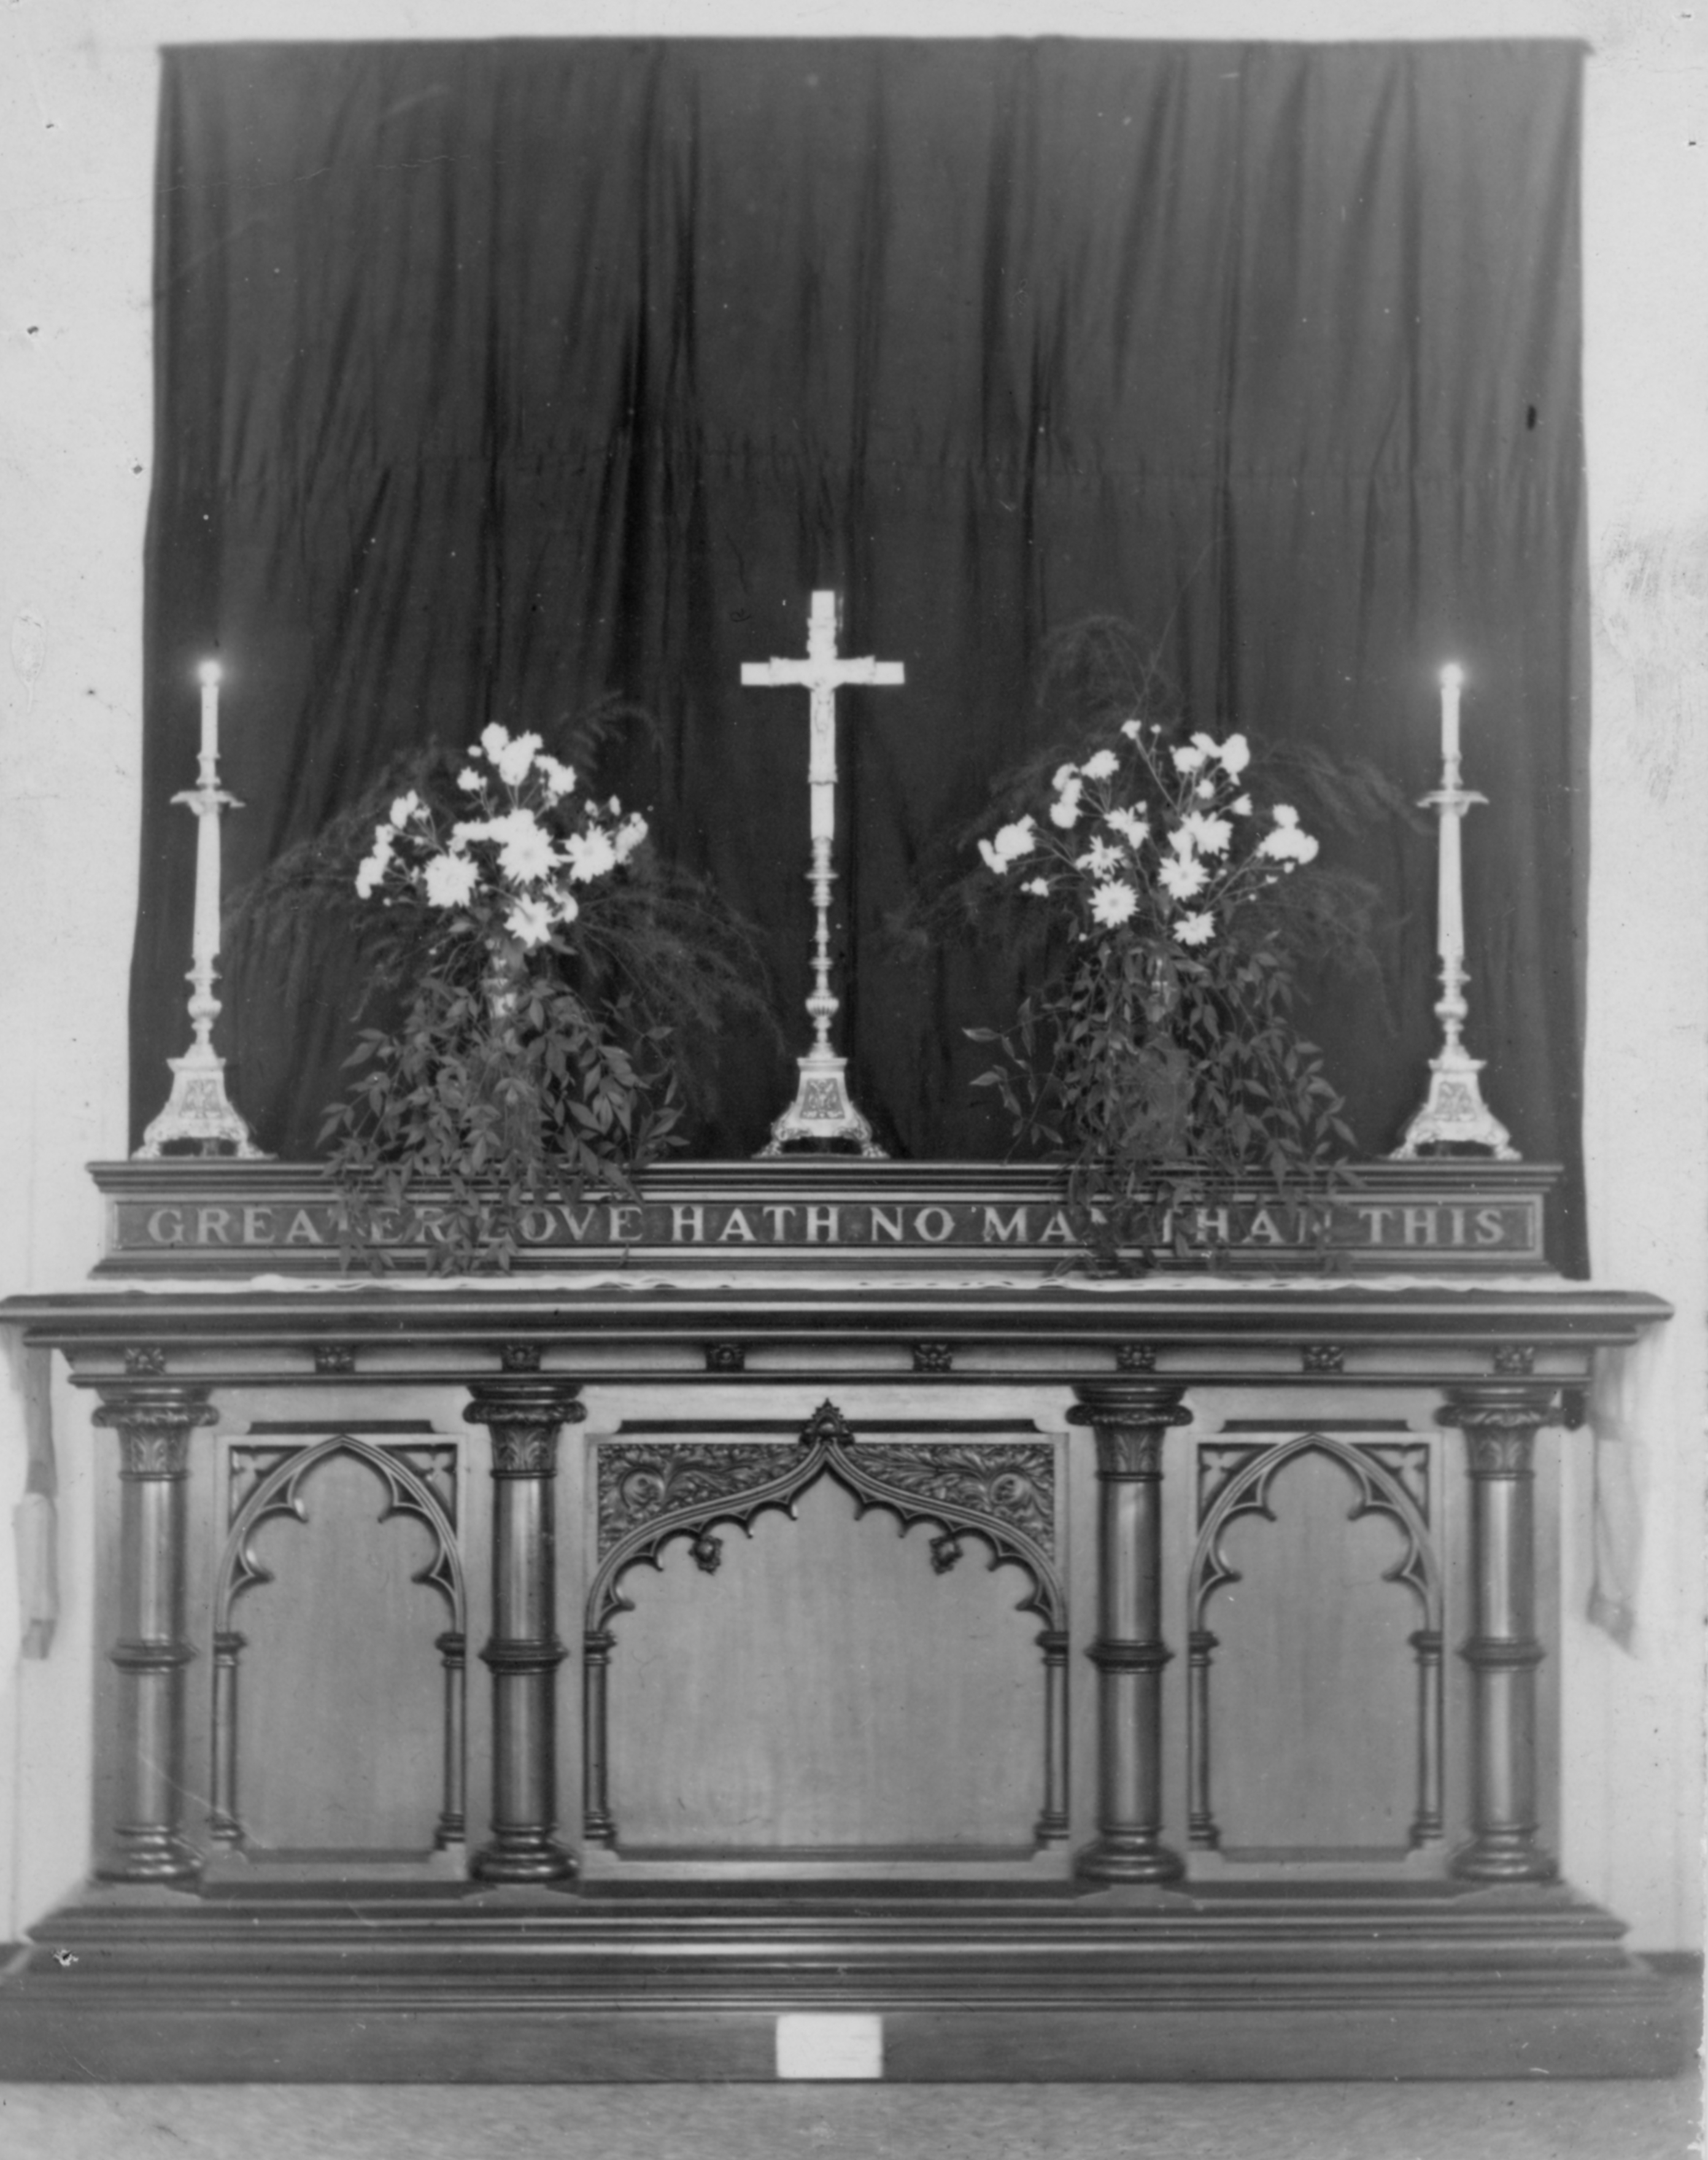
\includegraphics[width=1.\linewidth,center]{../images/cedarAltar1947.jpg}
\caption{Cedar Altar Christ Church Murgon in Memory of K G Wrigley, the gift of his family, 1947}
\end{center}
\end{figure}


Wrigley family again donated generously to the church as a later item in the 25 March 1947 Diocesan Archives record: `A faculty was this day issued to Christ Church, Murgon, authorising the introduction of a silver sanctuary lamp into the church.'\footnote{Diocesan Records and Archives Faculty Register 1947, Diocesan Archives, Brisbane} The lamp was dedicated at Easter that year. A plaque on the church wall reads: `In memory of George Edward Bromfield and Christopher Rodgers. Lit by Mrs Wrigley, Easter 1947. A gift of their relatives'. The lamp still resides happily in the church, but it has been altered from an oil burner, which had to be lowered by chains to be refilled, to electric power. The red bulb burns constantly.

A ` Special Meeting' of the parish was held in the Goomeri CWA rooms on 9 February 1947. It must have been considered `very important' as a typed copy of the minutes, rather than the usual hand-written ones, was pasted into the parish minutes book.

Rev Rodgers Burns was not present. Each centre was represented, being: R B Jeffries (Chair), Messrs Jones, Atkins, Gedge, Zahnleiter, Sempf, Quinn, H Stanton, Tate, Tapsall, Waldock and Sing with apologies from Messrs Pearson, R McIntosh, W Heathwood, P Stumm and W Short. Mr Jeffries stated that the meeting had been called for `\ldots the express purpose of discussing the attitude of the Diocesan representatives on the Presentation Board, Brisbane, and the apparent undue delay in the appointment of a Rector'. After lengthy discussion a motion was put and passed to write to the Presentation Board and `deplore the delay in making an appointment' and that they `considered the delay detrimental to the work and spiritual welfare of the parish.'

On a more general basis The various centres reported on their current financial positions. Mr C Wimberley had left the district and his former positions were filled by Mr Len Sempf as a Parochial Nominator and Mr Keen as Goomeri centre secretary.

The meeting carried a motion to purchase a replacement parish car, such purchase to be overseen by a five-member committee: Parish rector's and people's wardens plus Messrs Stanton (Goomeri), Waldock (Kilkivan) and M Maudsley (Windera). A letter of appreciation was to be sent to C Bischoff for making his own car available for use by the rector in the interim.

The old issue of `where the rector should reside' again emerged with a notice-of-motion by L Sempf to be presented at the next meeting suggesting that the rector should reside in Goomeri instead of Murgon.

The meeting concluded with Afternoon Tea prepared and presented by the Ladies of the Goomeri Guild who were accorded a hearty vote of thanks.\footnote{Kilkivan Parish Minutes, May 1947, Diocesan Archives, Brisbane, DJ 3 Box 2}

The 1947 Annual General Meeting was held on 25 May, as per tradition, in Goomeri CWA rooms. Twenty-two persons were listed as present, including now familiar names plus more interest being shown from outer centres with G C Quinn and L Eland (Boonara) along with Windera representatives, M Maudsley and C Noffke entering the scene on a regular basis. K Beitzel was listed a secretary.

Apologies: W Short, W Atkins and Reece (Bill) Mander-Jones. As the parish was in the hands of a locum tenens, the position of rector's warden was left open. All other office bearer positions were filled, and parish councillors nominated and elected -- Kilkivan five representatives; Murgon, four; Goomeri, four; Boonara, three; Windera, three; Cherbourg (CAS), one; Manumbar, one. The only business arising from the minutes related to the purchase of a new motor vehicle. As no significant progress had been made the matter was held over and left in abeyance.

The services register contains several notes of interest including the granting, by His Grace the Archbishop, of faculties. The Faculties Register confirms these as being for the new altar and another entry noting the founding of the Church of England Tennis Club, 29 May 1947.

Rodgers Burns actively participated in all aspects of ministry during his relatively short though events packed time of service. The 4 May 1947 services register indicates six services conducted that day -- five conducted by Rev Rodgers Burns and one by lay reader, W Atkins. An entry dated 11 May 1947 under Rev J Rodgers Burns signature seems to have been the last service conducted in the Parish by him. This is followed by a couple of isolated entries indicating occasional services conducted in Murgon by Lay persons, Mr Atkins, Murgon and Mr Doola of Cherbourg. Several blank pages follow.\footnote{Kilkivan Parish Services Register, 1923 -- 1947, Diocesan Archives, Brisbane, DJ 3 Box 2}

A page (not numbered) from the May 1947 minutes register refers to a parish council meeting held in the absence of a priest and chaired by the warden. Prolonged discussion on the purchasing committee's report resulted in majority decision and the motion of Mr Tate, seconded by W Atkins, authorising the wardens to proceed with purchase of a new Chevrolet motor car for the parish. This was carried unanimously. R Mander Jones' (Boonara) recommendation `that the matter of any finance required could be taken up with the diocesan secretary', along with Tate's suggestion that `a collector be appointed from each centre' for donations to this project. The meeting gratefully accepted Mr Gedge's generous offer of a \pounds60 pledge for 12 months interest free loan deposit for purchase. The wardens were requested to make every effort to obtain an increase in rebate from the dealer. A welcome afternoon tea, provided by the Goomeri Guild followed closure of the May 1947 meeting.\footnote{Kilkivan Parish Minutes, May 1947, p. 109, Diocesan Archives, Brisbane, DJ 3 Box 2} (These minutes were officially signed by Rev Alan Thompson at a 1948 parish council meeting.)
\balance

\printendnotes[custom]
\setcounter{endnote}{0}
\chapter{1947--1954 : Rev Alan George Thompson}
\nobalance

Alan George Thompson was ordained deacon in 1914 and a priest in 1915 after completing his Theological studies at Warminster College, UK. He travelled widely during his ministerial life, having served firstly as a Member of the Brotherhood of St Boniface in Bunbury -- a small village in Cheshire on the Shropshire canal until 1917. He then served as AIF Chaplain 1917-1919 before his traveling urge brought him as Priest-in-Charge in Western Australia till 1921, a short period on New South Wales, then into Queensland where most of the rest of his life was spent. Again, he covered a lot of territory and differing roles - Soldiers' Settlement Chaplain based in Fortitude Valley, Toowoomba, Mary Valley, Ipswich, several short stays in Brisbane suburbs until World War II again saw him acting as chaplain, this time to the AMF. Thus, he was not in the first flush of youth when service register entries commenced for Rev Thompson, on his arrival as Priest-in Charge of the Parish of Kilkivan, his signature appearing in the register of services 21 December 1947. In 1948 he was granted Rectorship of the parish which he retained until his departure from the area in 1954.\footnote{Diocesan Clergy Records, Diocesan Archives Centre,}

At a general meeting of the parish council soon after his arrival, the parish warden opened the meeting by welcoming Rev Thompson, hoping that `his stay would be a happy one and that the parish would build up again' under his guidance. Apologies from D Baulch, M Maudsley, P Seng, H P Stanton and L Eland were duly recorded.

The ever-present and concerning issue of finance, as alluded to in the previous chapter, was once again a meeting focus. In the nine-month absence of an incumbent, no monies had been forwarded by, or received from, any of the six centres. The parish appears to have drifted aimlessly, like a boat without a rudder, in the absence of a priest. Ministry (including funerals) had been provided almost entirely by a small band of lay persons. As a remedial action, the treasurer and wardens asked, firmly, that a one quarter's assessment from each centre be paid by 31 January. All agreed to this. The secretary was directed to contact the diocesan secretary requesting a reduction in parish assessment as a further effort to regain some financial ground. \footnote{Kilkivan Parish Minutes 1947, p. 108 l, Diocesan Archives, Brisbane DJ 3 Box 3} The parish assessment was seen as an added burden to a community which was already enduring the many sacrifices expected of all in the effort to maintain Australia's overseas war effort and so protect Australia from invasion.

The Diocesan response was that, regretfully, no relief would be able to be considered for the present assessment, but next year some consideration could be given, based on the current year's income.

The new Rector, Rev Alan Thompson chaired the 9 May 1948 parish AGM but did not present a rector's report, having only fairly recently arrived in the parish. The financial report was adopted subject to audit.The election of officers resulted in R Mander Jones (Boonara) accepting Rev Thompson's invitation to act as rector's warden. R B Jeffries was appointed as people's parish warden; Mr Monteith as auditor; parish nominators -- J W Tate, L Sempf, H P Stanton. K Beitzel was re-elected secretary / treasurer.

The parish council consisted of 12 elected members -- Quinn, Noffke, Maudsley, Stanton, Pearson, Zahnleiter, Tapsall, Waldock, Gedge, Livingstone, and Eland, along with the ex-officio members and the rector. Mr L Sempf spoke to his previous notice of motion `that the rector be stationed in Goomeri as it is (geographically) the centre of the parish. Much detailed discussion concerning running costs, distances involved from each of the two possible centres, the main hospital being situated in Wondai, and so on. Murgon parishioners received special mention for being the only centre to offer their private vehicles for ministerial use each Sunday. An `advisory only' committee consisting of the parish wardens plus one people's sub-warden from each centre was formed to further investigate general opinion.

A budget for the year ahead was presented. Financial obligations to basic running costs - stipend, phone, synod assessment etc -were estimated at \pounds556 which included an overdraft of \pounds20. Of foremost importance to the budget was the `new car' project. The committee which had been appointed for this purpose had used its authority in this regard and proceeded, through church member and local car dealer, Mr Bischoff, with negotiations for the purchase in the absence of an incumbent Their decision was no doubt influenced by Mr Gedge's (gratefully accepted) offer of a \pounds60 interest free loan for twelve months as a deposit, and by Mr Bischoff's to service the vehicle. By December 1947, a letter to the Diocese stated that as `the parish can raise \pounds200 almost immediately', they wished to apply for an overdraft of \pounds450 at the National Bank to complete the purchase of a `Stylemaster' Chevrolet. This overdraft carried the requirements that it be reduced by at least \pounds150/pa over a three-year period. At this May 1948 meeting, to cover this expenditure fully, the vehicle's purchase price of \pounds685 was allocated in quota form to each centre: Murgon \pounds216; Kilkivan and Goomeri \pounds161 each; Boonara \pounds107 and Windera \pounds40.\footnote{Kilkivan Parish Minutes 1947/1948, Diocesan Archives, Brisbane DJ 3 Box 3}

The matter of increased costs incurred in servicing the Cherbourg community was discussed. A motion by R Mander Jones and seconded by P Seng authorised the secretary to contact Canon Massey in this regard and seeking assistance. It further pointed out that Mr W Atkins regularly attended to church matters there, usually riding his bicycle there and back. Messrs P Sing and R Mander Jones asked that `an appreciation for Mr Atkins' good work at Cherbourg and all who had made their cars available for the Rector while the parish was without one.' Mr Jeffries and Mr Atkins responded with `If a job is worth doing, it is worth doing well!'

Current parish members in fairly significant numbers recall Rev Thompson's incumbency with a deal of warmth. Being slightly vision impaired from desert sand in the Middle East, on his arrival in the parish, Rev Thompson was greeted by Mr Bernard ``Bill'' Gedge who, subsequently, frequently drove him around the Parish in a brand new, big heavy Chevrolet sedan. As recalled by Mr I D (Mick) Kapernick, they were often bogged in the wet weather, particularly in going out to Windera -- a telling comment on the road conditions at the time. Local reminiscences paint a fond and positive picture of Rev Thompson referring often to `his little eccentricities', such as singing, \emph{loudly,} the alternate tune while the congregation and the organist ploughed on with the familiar one. He is also renowned for using his strong, booming voice on occasion if he felt the congregation might be falling asleep in a 2.00 pm service on a long, hot summer's afternoon. The problem was that occasionally he awakened sleeping babies as well as the adults, much to the distress of the mothers who then had a crying child to pacify, though an escape to the shade outside may have been a welcome interlude. He is also credited with using a whole jugful of water -- often a little cooler than tepid -- to douse babies presented for baptism, not so well received by the little ones in winter! The life of the parish continued in this congenial fashion providing a needed sense of security within the fabric of a war-tarnished environment.\footnote{Anecdotes collected during interviews and research (M McIntosh)}

15 August 1945 was a momentous day for Australia marking the end of World War II. Certainly, it was a day of note for Murgon's community who now eagerly awaited the return of the final batches of local troops. Although overseas conflict ended, the ongoing effects on the home countries remained. While Australians civilians, generally speaking, did not suffer as much as many other populations (eg. the UK), the impact on our home front remained significant for several more years.

A 1949 notation mentions `Ration Coupon Day' on 27 November and a street stall operated by the Murgon Guild ladies being held to celebrate the end of wartime rationing and to provide a needed boost to finances and to morale with events taking on a more `normal' face.\footnote{Parish of Kilkivan Service Register, 27 November 1949, Diocesan Archives, DJ 3 Box 2} The rectory garden, happily attended by Rev Thompson throughout his stay in Murgon (most likely with the assistance of Bill Gedge) provided fruit and some vegetables which he liked to distribute to any of the ladies of the parish who were willing to turn them into jams and pickles for church stalls and catering purposes.\footnote{Murgon Ladies Guild Minutes and Cash Book 1940-1966 entries. Parish files, Murgon.}

Rev Thompson was never seen dressed in anything but his Khaki army style clothing -- another of his apparently endearing eccentricities. Being a bachelor seems to have triggered the `mothering instinct'. The ladies of the parish took him under their wings with one who did all his washing and ironing - and there were many others, several in each centre, who vied for the honour of feeding him in the times between services in each of the centres. On occasions such as the gap between an afternoon service and one around 7.00 pm in outlying centres, he was provided with a bed for a well-deserved rest before his evening meal, both intended to sustain him till bedtime.

Apart from all of this, in addition to the regular run of services, Rev Thompson was very keen to instruct children and ensured there were Sunday School Classes in all the centres, conducting them himself if necessary, adding extra working hours to already crowded days. At Windera, church services and Sunday School classes were conducted in the old Windera Community Hall. Every Christmas each child was given a prize book, chosen, and signed by the Rector. He loved `Westerns' and his choice of prize books certainly showed where his recreational reading interests lay, though some may question the spiritual relevance of titles such as `Gun Law'. The Parish's Sunday Schools prospered with up to 100 children attending at various centres with Murgon at the forefront. Credit must also be given to Mr Gedge for his enthusiasm and generosity of time in providing teaching, as well as being Murgon's Sunday School superintendent and recruiting a dedicated band of committed teachers.\footnote{Murgon Services Register, 27 November 1949, Diocesan Archives, DJ 3 Box 2}

Ross Waldock writes of the Sunday School: `My first memory is of Sunday School in 1953 (I think) before I started school. Teachers were Mr Bill Gedge, Miss Edith Gedge and Mr Bill Atkins (who rode a bike). I hated Sunday School -- John Mickan teased me till I cried. Mr Gedge took me home to Mum and Dad -- but I was sent back next week. Sunday School was held in the vestry and in the church. The Christmas break-up was in the Town Hall supper rooms -- fantastic!\footnote{Personal notes supplied by Ross Waldock.}

During these years Murgon church, and indeed the whole parish, could be described as active, enthusiastic and dedicated, with regular sacramental services of confirmation, baptism and marriage. The recurring problem of having adequate finances to cover all contingencies was ever present.

In 1948 Rev Charles Tunstall, after nine years as Rector of St John's, Biggenden, retired to McLucas Street, Murgon. As is always the case, clergy persons never `retire' completely and his name began to appear as the officiating priest in the Murgon church's services register, an undoubtedly welcome assistance to Rev Thompson.\footnote{Diocesan Clergy Records, Diocesan Archives Centre, Brisbane}




\begin{figure*}[!htb]
\begin{center}
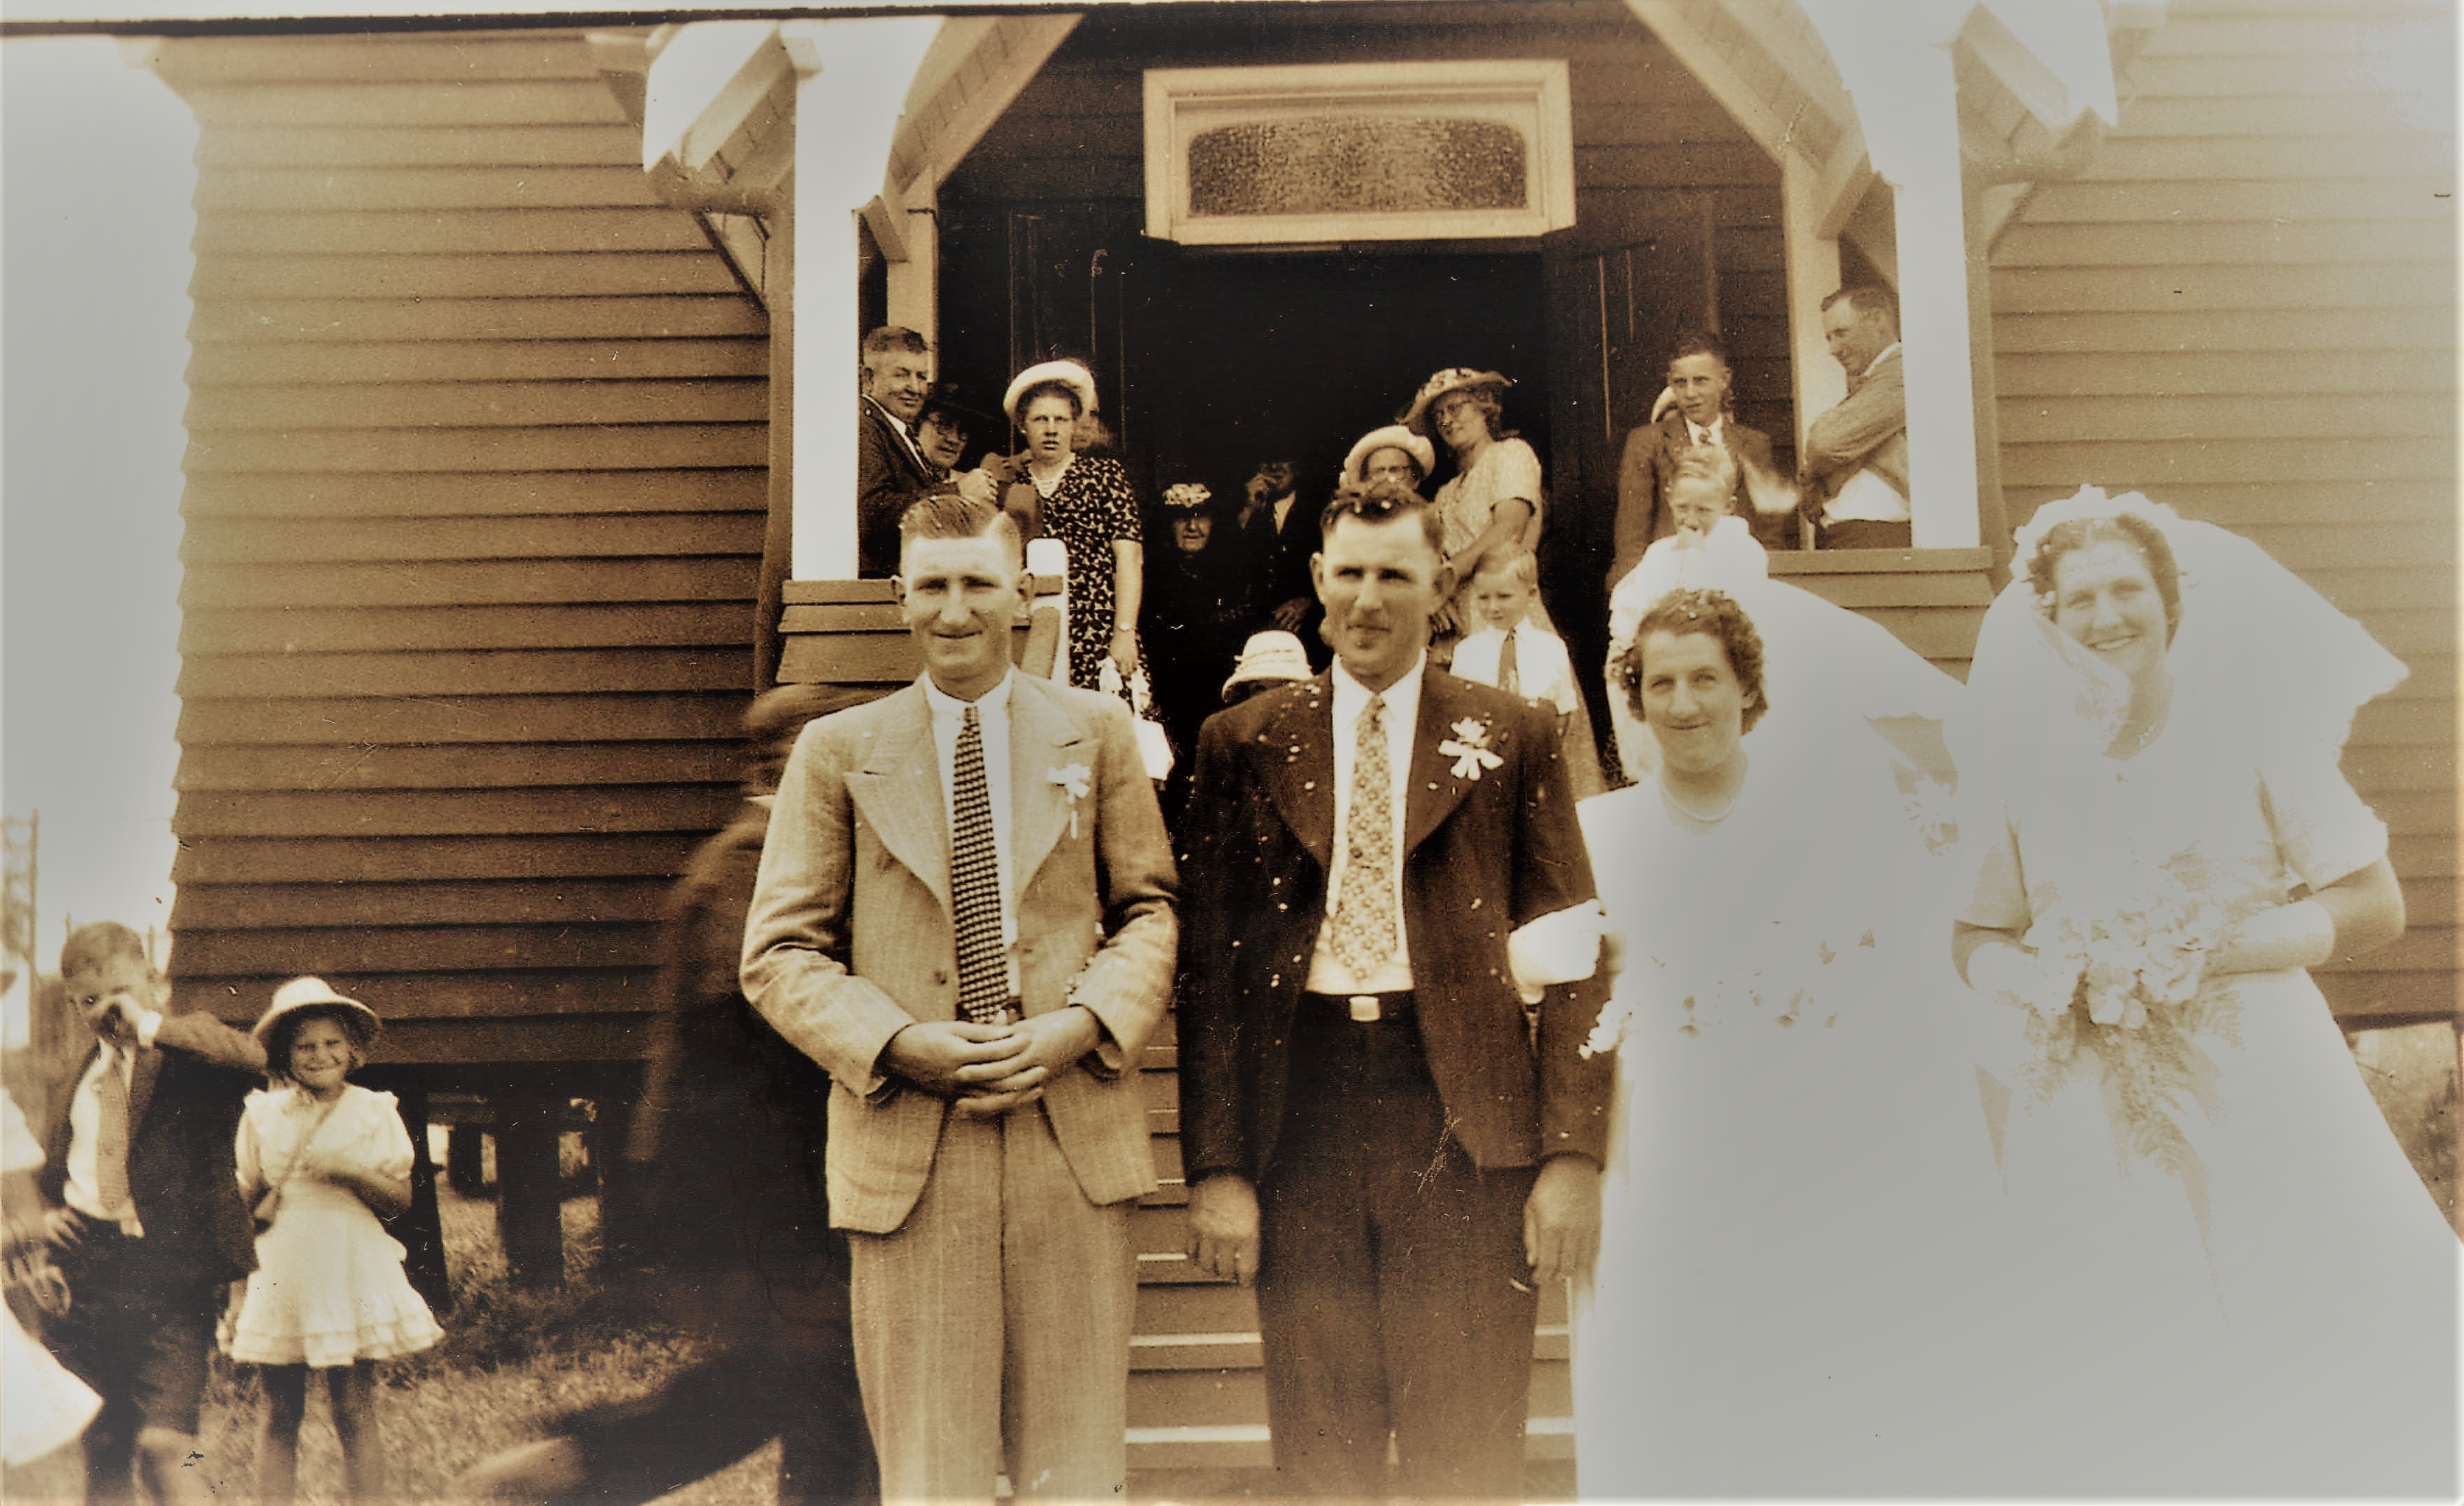
\includegraphics[width=1.\textwidth,center]{../images/JackDennienGladysMorgan12Jan1951.jpg}
\caption{Jack Dennien and Gladys Morgan 12 January 1951}
\end{center}
\end{figure*}


Social, community-based activities were greatly encouraged with a view to presenting the parish to the general public as a vibrant, welcoming community open to all as well as a means of augmenting funds. As an example, a call went out for young women to participate in a Debutante Ball being organized by Church of England volunteers, including Mrs Seng. The successful advertising campaign brought a bevvy of beautiful young ladies to the Murgon Town Hall. As reported in 7 October 1950 \emph{Courier Mail,} Brisbane, Missies Merle Towne, Pauline Bennett, Heather Waldock, Alma Beutel, Heather Evans, Norma Towne, Veronica Nichol, Dulcie Holznagel, Daphne Raddacliffe, Winnifred Noffke, Elizabeth Reese, Beryl Harm and May Solomon - and their equally handsome young escorts to the Murgon Town Hall where they were presented to the Venerable Archdeacon Frank Knight.\footnote{\emph{Courier Mail,} Brisbane, 7 October, 1950}

Entries in the parish services register and articles from the \emph{Church Chronicle} both indicate a proliferation of activities during 1952. The first of three successive monthly articles in the diocesan news publication occurred in March where the rector announced that `Canon Massey is visiting this Parish for Mothering Sunday (23 March). I have asked him to Bless the Memorials in Christ Church.'\footnote{\emph{Church Chronicle,} March 1952, Diocesan Archives, Brisbane} As described in the previous chapter, the cessation of hostilities and the coming of peace in 1945 moved the grateful and grieving Murgon community to give visible expression in the form of various memorials in the church. The most forward-looking venture, and indeed a large step in faith, considering the expense involved, was the decision to install a stained glass, leadlight window in honour of the local fallen and as a Peace Memorial in the wall of the church behind the altar.

While the parish services register for March carried many memoranda notations indicating heavy rain interrupting some services in Kilkivan and Goomeri, a week later it also confirms that Rev Canon R B Massey, (organizing secretary of the Home Missions Board) was present to `bless the memorials in the church'.\footnote{Parish of Kilkivan Services Register, 30 March 1952, Diocesan Archives, DJ 3 Box 2} Again, anecdotal evidence indicates that the said `memorial' was indeed the beautiful war memorial window. This striking Silky Oak framed tribute to the local `fallen servicemen' measures 1.46m x 1.18m, is formed in three sections and bears the inscription `To the Glory of God and in Thanksgiving for Peace, August 1945. These windows are erected by the Parishioners of Christ Church

Murgon'\footnote{Photos and information from Diocesan Archives Centre, Brisbane and courtesy Donna Hindley, Murgon.}. A `Sung Eucharist' at 11.00 am, Murgon, was a highlight on this last Sunday of March and included a `retiring collection for Red Cross'. An 8.00 pm parish council meeting in Goomeri followed.

More memoranda items from1952 included the admission of nine candidates to GFS and the `making of one associate' during September and the October events including a visit by the Rural Dean, E R Crittenden who received Debutantes in the Murgon Town Hall and a Kilkivan children's fancy-dress ball. During November Redgate Sunday School held its prizegiving party and Hostel Prizes were also presented to `McCosker and Twible'. Boonara and Kilkivan followed suit also in November, with both events following services of evensong.\footnote{Parish of Kilkivan Services Register, September and October 1952, Diocesan Archives, Brisbane, DJ 3 Box 2}

1953 Services Registers: 3 May, the parish hosted an Archdeaconal visitation by the Venerable F B C Birch for the blessing of three pictures which had been donated to the Murgon church. Following local custom, local AGMs were held at each centre prior to the Parish AGM, which was held on Wednesday 20 May at 7.30 pm following a service of evensong.\footnote{Parish of Kilkivan Services Register, 3 May and 20 May, 1953, Diocesan Archives, Brisbane DJ 3 Box 2S} The parish hosted the 18 October 1953 visit by Archbishop Reginald Halse where he officially dedicated `the new work' which involved extensions to St David's church, Boonara, dedicated the new front gates in memory of John (Jack) Mander-Jones (killed in action 1942) and consecrated the burial grounds within the church ground perimeters. These had been a Jones Family private cemetery but now became an official Church of England cemetery area.\footnote{St David's, Boonara, centenary booklet p. 15}

The main events for Murgon in December 1953 are neatly summarized in the \emph{Church Chronicle.} The Murgon GFS break-up party was an outstanding success with around 50 present. Presentations were made to president, Miss B M Delpratt (BA), and secretary Miss Maureen Olsen. Murgon Sunday School's prizegiving followed a `reverential' Advent 2. Prizes were distributed and presentations made to Mr Gedge (superintendent), Miss Edith Gedge and Mrs Beinke (organist). Thanks were extended to all who made the 4 December Christmas Tree event such a hilarious event, with a special mention to Mr Richardson who acted as Santa (Saint Nicolas).

Mr Thompson advised that the next parish council meeting was scheduled for 31 January 1954 at 2.00 pm in Goomeri. Women's Guilds were asked to send at least two representatives.

Rev Thompson's article ended with a parting message for the whole parish:

\emph{`I feel the time has come for me, in the interests of the Church, to make place for someone younger than I am. To make this decision has not been easy. Most people when asked what the happiest time of their life has been, refer the questioner to their childhood days. The happiest time of my life has been whilst Rector of Kilkivan Parish. This has been effected by the loyal co-operation and kindliness of the people whose souls have been entrusted to my care. May my successor be as happy as I have been!}

\emph{A happy and prosperous New Year to you all'.}

The final diocesan news publication for Kilkivan parish by Mr Thompson was on 14 February 1954. His `last notes' were written from the rectory in Hamilton, Brisbane, where the spaciousness, `exquisite carpets and curtains', `sumptuous furnishings' and spacious verandahs made him feel like being `in Buckingham Palace' with gardens `reminiscent of fairyland', not to mention the abundant access to running hot and cold water -- what a contrast after the rather run-down premises in Murgon. After waxing lyrical he went on to inform that his next `place of abode' would be Charleville where he would `assist members of the Brotherhood which has its headquarters there, but not be a member of that self-sacrificing company of priests'. With a few brief notes covering the Goomeri Sunday School end of year celebrations and Murgon's Christmas Dance, he concluded with \emph{`Goodbyes will be too painful, so we will be casual when parting, as Mr Stanley was when he found Dr Livingstone in Central Africa after searching for him over a long period, under trying conditions. He simply said, ``Dr Livingstone, I presume''. For the last time -- AGT'}.\footnote{\emph{Church Chronicles} 1 January and 1 and 14 February 1954, Diocesan Archives, Brisbane}

His final entries in the parish services register were on 28 February 1954. His last day's duties covered four centres -- 7.30 am, Murgon; 10.45am. Windera; 2.00 pm, Boonara and 7.30 pm, Kilkivan. Diligent to the final minutes of his tenure! He signs off with the bland notation: `Rector resigns and leaves for Brotherhood headquarters', 4 March 1954.

An archives-held letter signed by J Tate as secretary for the parish nominators, voiced sincere regret at Thompson's departure and glowing praise for his work as `\ldots unsurpassed by any of his predecessors \ldots{} improvement in parish immense \ldots{} sermons a delight to listen to \ldots can leave the parish feeling very proud.' The letter continued with arrangements towards the acceptance of Rev J Kruger as Vicar.\footnote{Diocesan Correspondence, 16 January 1954, Diocesan Registry Files 1954}

Clergy records indicate his final years were spent at St Alban's Clergy House, Weinholt Street, Auchenflower.\footnote{Diocesan Clergy Records, Diocesan Archives Centre, Brisbane} It is seldom a parish is blessed with a priest that `everybody loved' and who seemed to so thoroughly enjoy and appreciate absolutely everything. God bless you Rev Alan George Thompson.
\balance

\printendnotes[custom]
\setcounter{endnote}{0}
\chapter{1954--1956 : Rev Jack Kruger}
\nobalance

The arrival of Rev Jack Kruger (1923-1978) introduced a vibrant and busy time for the Church of England in Murgon. The youthful enthusiasm of this 31-year-old priest was contagious. Rev Thompson's parting statement that the parish was ready for `a much younger man' proved prophetic in spite of the tears which accompanied his departure. Rev Kruger had the reputation of being a `good, down to earth Aussie'\footnote{Kilkivan Centenary Booklet, p. 14} and quickly gained the support of all. He was very well regarded throughout the parish from the very beginning. Having served as vicar of the parish of Mary Valley for two years before his promotion to rector of Kilkivan Parish, he had been introduced to the rigors of country parish service. Diocesan Registry Files, 1954, contain copies of documents and correspondence between the parish nominators, J Tate, L Sempf and HP Stanton, and the diocesan registrar, Mr St John, regarding the appointment of Rev Kruger to the parish.

By 17 February the minimum stipend payable was \pounds625. The parish's agreement to this figure, along with the rectory accommodation, a 1953 Holden Sedan parish car plus all running costs and repairs was offered in communications with the Diocesan officials. All necessary paper work for the appointment of Rev J Kruger was also completed by 15 February 1954. As mentioned in the previous chapter, the rectory was as `the rather run-down premises in Murgon'. Some minor repairs were carried out but much remained to bring the premises up to acceptable standards. It seems this did not receive attention as fully as was required, although the Guild is credited with supplying some blinds, some cupboards and `Lino for the purchase of a motor mower. However, Rev Kruger's buoyant approach was not daunted.

The first services register entry to his name was for 7 March 1954 where he signed in full, ``Jack Kruger'. Thereafter, the simple initials, JK, was all he ever used. Mention is made of a 6.30 am special `Lady Day Mass' for 16 communicants on 25 March. Mothers Union members frequently used bus transport to travel to special joint services in other parishes for these celebration days.\footnote{Kilkivan Parish Services Register, 7 March 1954, Diocesan Archives, Brisbane DJ 3 Box 2} Rev Kruger, following in the footsteps of his predecessor, was a diligent contributor to the Diocesan issued \emph{Church Chronicle}, a well-received and anticipated publication in this parish. Written late in March 1954 in time for the April edition, he mused on the privilege for those in attendance at the `very special service in St John's cathedral, Brisbane, in honour of Her Majesty the Queen and the Duke of Edinburgh, Prince Philip,' during their Australian tour. He expressed his gratitude and thanks to Rev Thompson `for seeing to the rectory lawns and leaving the car in such good order'. He gave forward notice of the Easter services, the parish AGM, 16 May @ 10.45 in Goomeri, and the availability of Lenten Boxes, as well as encouraging parishioners to support the Easter Play to be presented by the local GFS group.\footnote{\emph{Church Chronicle,} 1 April 1954, p. 123, Diocesan Archives, Brisbane}

Rev Kruger's official `Introduction and Induction' was conducted by Canon ER Crittenden in an 8.00 pm service in Murgon on Thursday 8 April 1954, thereby marking the beginning of a two-year, event-packed incumbency. Over 100 people attended.\footnote{Kilkivan Parish Services Register, 8 April 1954} The occasion was written up in the May \emph{Church Chronicle} where the rector fondly recalled that the Gympie-based Rev Crittenden had conducted a similar service for him in the parish of Mary Valley two years earlier. The Murgon Ladies' Guild's appeal for contributions to the up-coming Annual Fete in the Murgon Town Hall was advertised.\footnote{\emph{Church Chronicle,} 1 May 1954, p. 155} Support was forthcoming and, `in spite of the inclement weather' the 8 June event netted \pounds114'.

The fete was officially opened by Mrs Florence Bjelke-Petersen, Kingaroy, wife of the then local member of parliament and later premier, Sir Joh.\footnote{\emph{Church Chronicle,} 1 July 1954, p. 218} July news continues: At the parish AGM held in Goomeri, there was concern for the state of parish finances. Though in an overall `fairly sound' position there was a large overdraft to be dealt with. Various suggestions for an `all-out effort' were put forward. Rev Kruger took a proactive approach and along with office bearers, including the re-elected D Jeffries as People's Warden and C V Lord (Boonara), secretary and treasurer, he employed leadership talents in organizing several of the suggested money raising events. These included Amateur Trials (Talent Quest event) and a Motor Gymkhana -- both fresh approaches aimed at promoting general and wide-spread community involvement.

The Amateur Trials received first attention with events planned for and supported by participants from all parts of the area. Murgon, Windera, Goomeri and Kilkivan centres actively planned and organized events over August and September, uncovering a wealth of largely untapped talent throughout the district. (On a personal note, I recall taking part, as a newly turned 13-year-old, playing a piano solo ``Dreams of Youth'' in the Windera/Cloyna organized event, in the Cloyna Hall.

My father also did his `strong man' tricks, bending iron rods across the back of his neck and on his bottom jaw. Neither of us made the finals). Finalists from these wonderful, fun-filled lead-ups gathered for the culmination in Goomeri's Hall of Memory on 22 September for a `finals night never to be forgotten'. That night alone made over \pounds180. Local businesses were gratefully thanked for sponsoring its broadcast over local radio station 4SB, which was compared by Mr George Parker, a 4SB announcer. The euphoria of success led to the voicing of `plans' to `do it again next year' being forthcoming.\footnote{\emph{Church Chronicle,} 1 November 1954, p. 346}

While the main emphasis was on these talent quests during this time, forward planning in November 1954 went ahead for the Motor Gymkhana with 5 March 1955 being fixed for its staging in Goomeri, following an initial planning meeting in October where all were encouraged to attend and to `bring along your ideas and suggestions'.\footnote{\emph{Church Chronicle,} 1 October 1954, p. 315} The event was coupled with an underlining parish appeal emphasising efforts to `remove the overdraft'. Local areas pitched in during this time by organizing further fundraising and social events.

Reflecting the popularity of ballroom dancing at the time, prominent among these were imaginative approaches such as the 2 October Ballerina Ball in the Tansey Hall and Goomeri's Annual Ball in the town's Memorial Hall also in October. A very happy, and purely social, combined guilds get-together was also held in Murgon during November. The usual Guild efforts of running street stalls and functions catering also need to be acknowledged along with `pleasing attendances' at church services throughout the parish. October is remembered in Kilkivan as the time `when the lights came on' -- referring to the connection to the electricity supply grid and the dedication by Rev Kruger of a generous donation of lights for the church by the Sempf family in memory of departed family.




\begin{figure}
\begin{center}
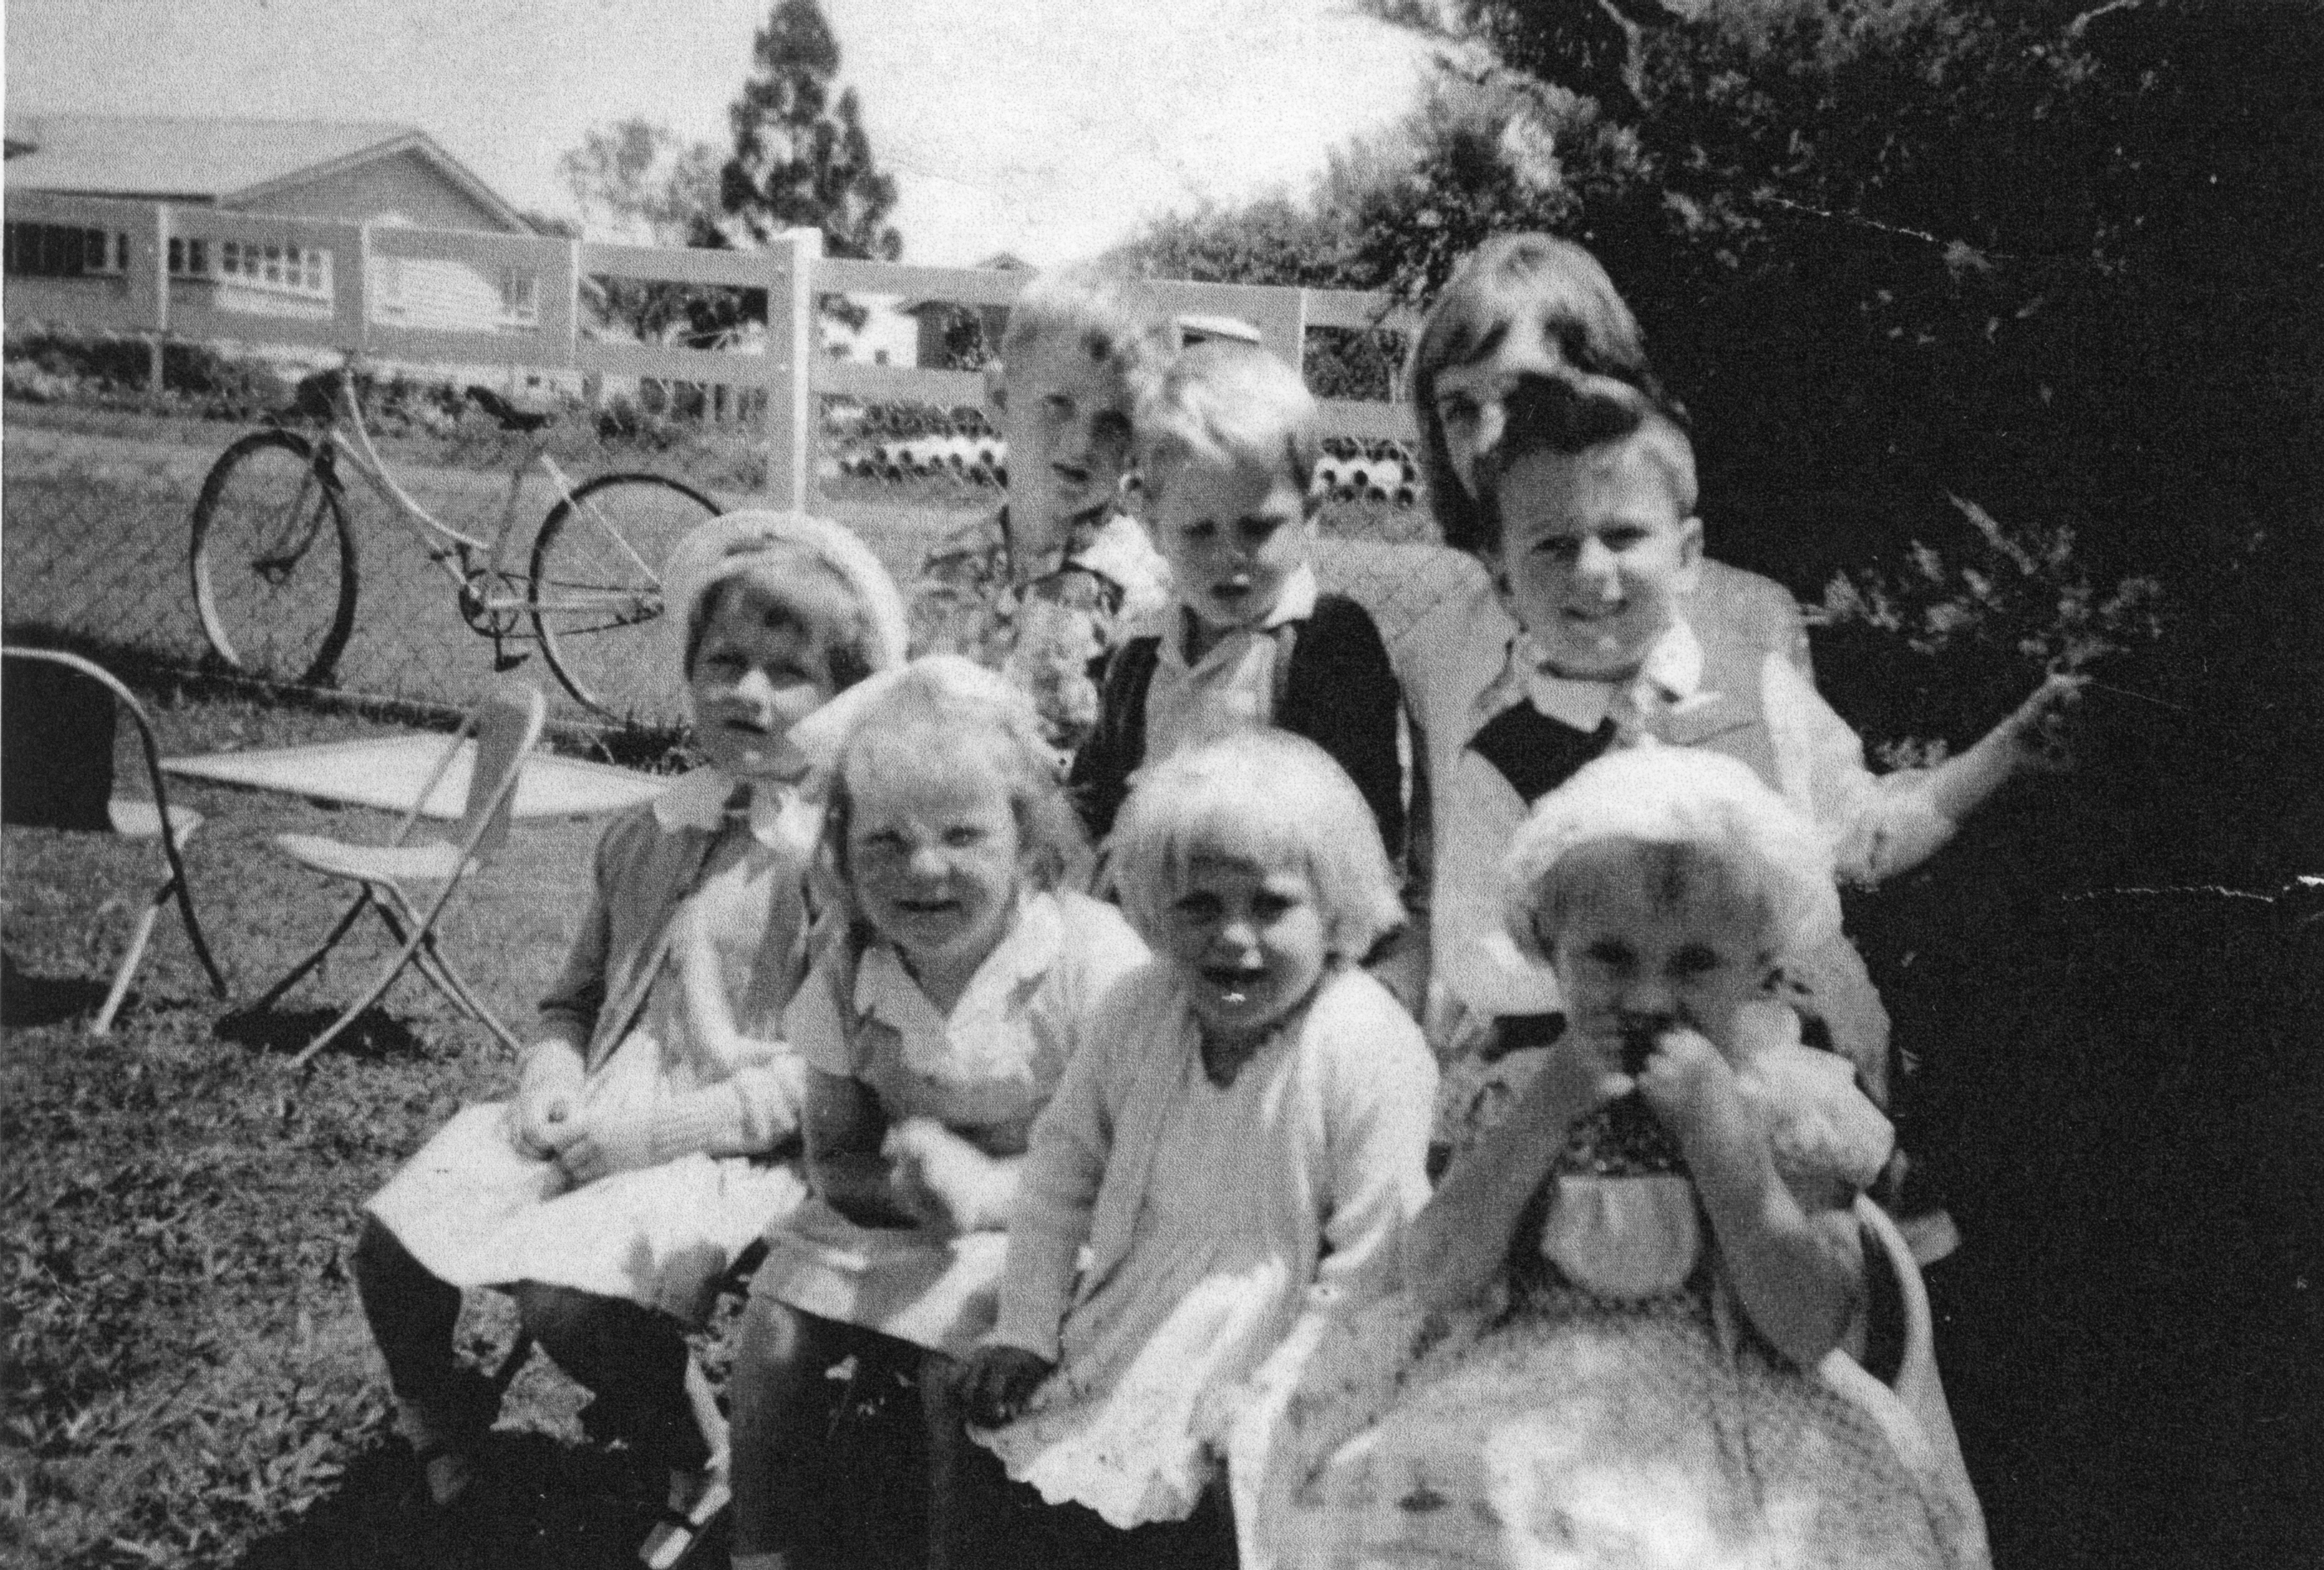
\includegraphics[width=1.\linewidth,center]{../images/sundaySchoolMurgon.jpg}
\caption{Sunday School, Murgon}
\end{center}
\end{figure}


Windera congregation was complemented for attendances which `underlined the necessity for a church (building) for that centre' adding that `they desire only a small building and not much debt'.\footnote{\emph{Church Chronicle,} 1 August 1954, p. 250 ff} By the October edition of the \emph{Church Chronicle} Rev Kruger was able to report the purchase of two blocks of land for this purpose and that the `aim was for the church to be built in 12 months.' October was reported as `a month of very bad storms' with Kilkivan church being partly unroofed. Mr Jack Krebs and his team of builders was on the scene early the next morning and the work completed in a couple of days. Thankfully, insurance monies covered the cost of repairs.

By December, with plans for Christmas events and the rector's annual holidays were well underway. Parishioners were directed to the \emph{South Burnett Times} for service details for Christmas and January services. During the rector's absence the parish would be `attended by the kind offer of Rev Charles Tunstall', previously mentioned as being retired and residing in Murgon.\footnote{\emph{Church Chronicle,} 1 December 1954, p. 378}

With 1954 drawing towards its close, rector and parishioners were able to reflect on a year of progress in the growth of spiritual development leading to physical evidence of this in so many ways. The Venerable Archdeacon Crittenden again graced the parish during Bible Week in September and was guest speaker at the Murgon Town Hall where he addressed a large crowd on `The Authority of the Bible'. Necessary repairs and improvements to the rectory had been carried out mid-year. Several large anonymous donations had been forthcoming for different projects. Electricity from the `grid' was beginning to be connected in the area instead of local town power plants. Kilkivan was the first centre to be connected to this system. Additional schools had been added to the rector's visiting list, and, although as always happens, concerning or sad occasions such as illness and the passing of valued members had occurred, on the whole, it was a year to be celebrated.

The momentum continued into 1955 with grid-connection for electricity supplies progressing well. Windera Guild minutes, a copy of which has the date of May 1955 printed above the hand-written record deal with the plans for the new church of St Katharine's (the originally chosen name), stump-capping ceremony, which was to be a `festive occasion' with, flags, stalls and a sumptuous Afternoon Tea.\footnote{Windera Ladies Guild minutes, Diocesan Archives, Brisbane DJ 3 Box 3} Letters in the diocesan registry's correspondence file as well as a the record in the an old, faded and damaged, Parish Service Register, assumed to belong to Kilkivan, located by diocesan archivist, Glenda Murrell, the stump-capping ceremony for `the proposed St Katharine's Church at Windera' took place in 1955.




\begin{figure}
\begin{center}
\includegraphics[width=.9\linewidth,center]{../images/weddingMurgon1955.jpg}
\caption{Wedding, Murgon 1955}
\end{center}
\end{figure}





\begin{figure}
\begin{center}
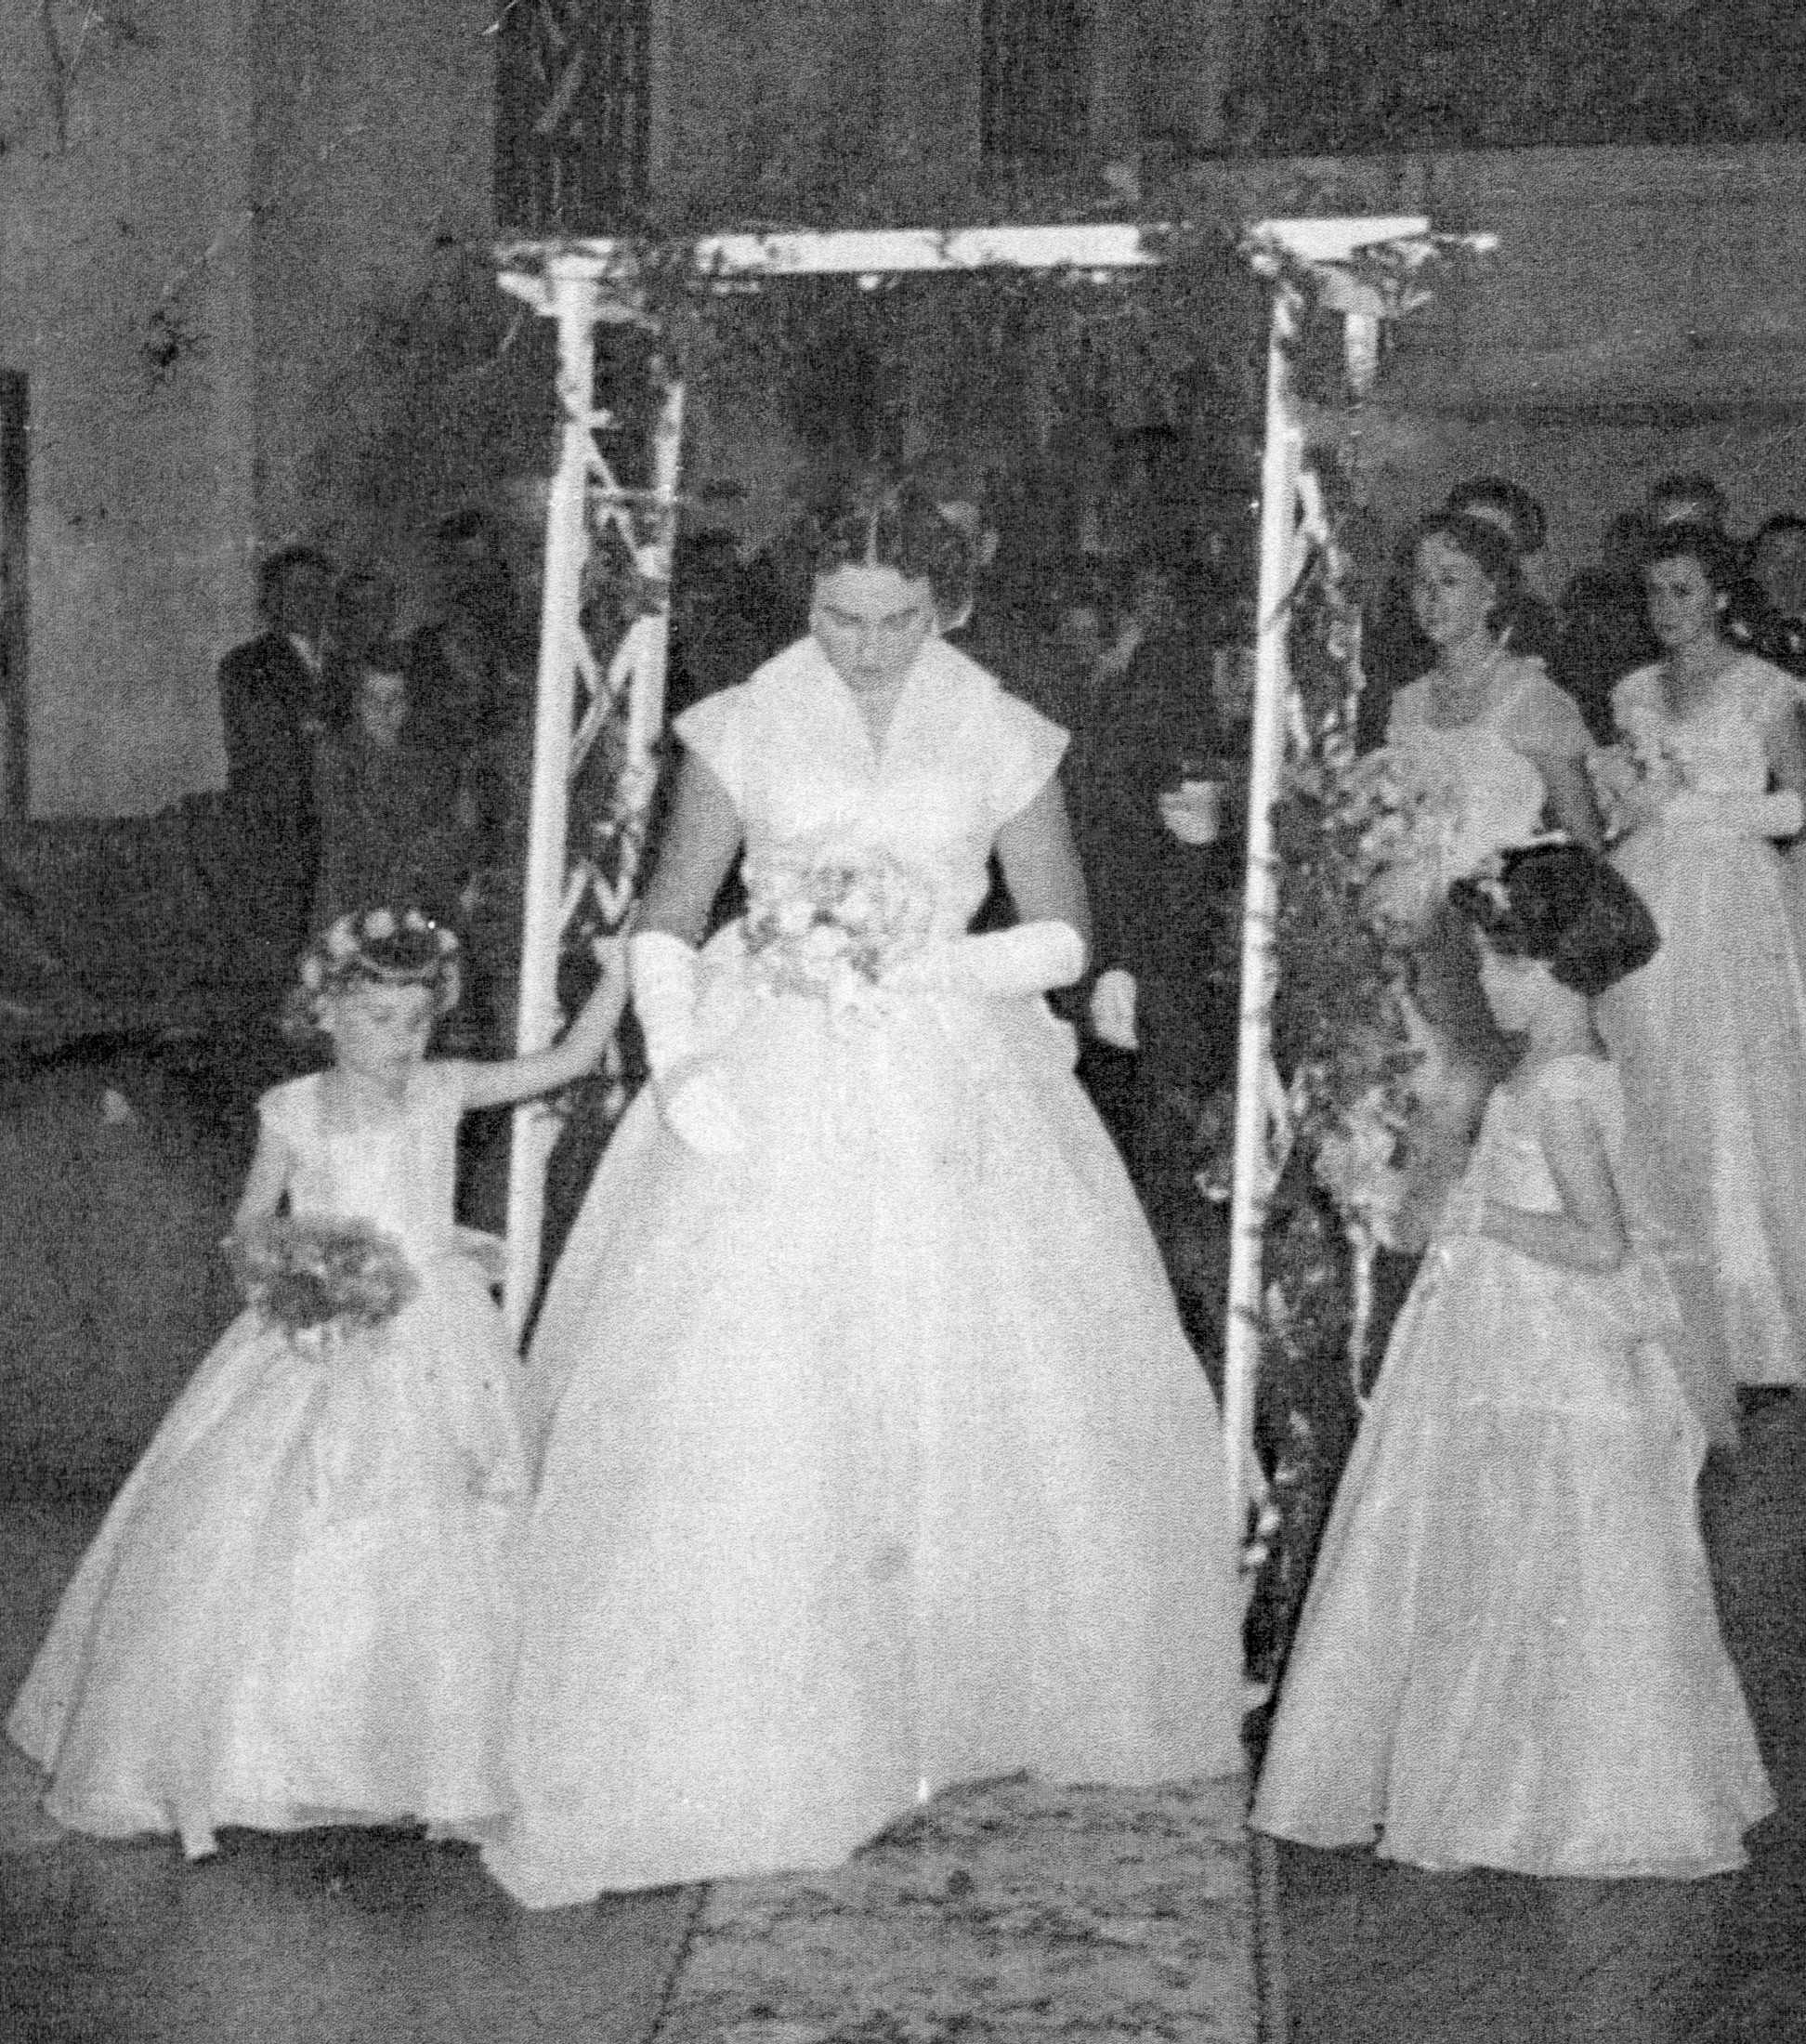
\includegraphics[width=.9\linewidth,center]{../images/debBallMurgon.jpg}
\caption{Deb Ball, Murgon, ca 1956}
\end{center}
\end{figure}


The comprehensive local notes in the 1 December 1955 \emph{Church Chronicle} speak of the donation to Murgon church by the centre's guild -- a picture in memory of Mr Beinke `who for a number of years was organist at the church'. Prior notice was given of a Carols Service by the choir in Murgon on 18 December and duly confirmed by the service register entry of that date. Timber for the Windera church was gradually being purchased, endorsing the hopes of starting the construction early in the new year. Electricity was now connected to Boonara church with thanks going out the generous person who completed the installation. The rector was exceptionally pleased with the newly-formed Men's Committee who had voluntarily painted the church and lined the vestry, providing great assistance to the parish and the local ladies guild funds reserves.

Throughout the year the usual occasional services of weddings, baptisms and funerals continued. With the Methodist-run students' hostel just two doors down from the church, there was an `on-tap' supply of high school-aged students for confirmation lessons. And so the forward momentum had continued there, and indeed, throughout the entire parish, for the remainder of 1955.

Rev Kruger concluded his December notes with `My wife and children have now returned to the rectory. Mrs Kruger is feeling really well again and we wish to express our thanks to those people for their good wishes and kind acts.'\footnote{\emph{Church Chronicle,} 1 December 1954, p. 367} Sadly this optimistic entry was followed by the dear lady's tragic death, recorded in a simple one line entry in the services register: 16 December, 7.30 am, attendance 2, Requiem for D P Kruger, signed JK. Clergy Records record her as `Spouse Dorothy Patricia (nee Hardy). Died 1955.\footnote{Diocesan Clergy Records, Diocesan Archives, Brisbane}

While most parishioners were either totally unaware, or knew very little of this devastating event, it was a difficult time for the wardens of the parish and those closely associated with the rector as they endeavoured to protect his privacy while he bravely carried on and faithfully completed the full round of four tightly time-scheduled Christmas Services beginning with a Sung Eucharist in Murgon at midnight, an early service at Kilkivan followed by Boonara, then 11.00 am at Goomeri. Windera was catered for by Rev Chas Tunstall at 8.30 am. In all 139 people received their Christmas Holy Communion. Services thereafter were conducted by Rev Tunstall (occasionally assisted by Mr Stuart James, a lay person locally stationed with the Department of Agriculture and Stock) beginning 1 January 1956 while Rev Kruger was on official compassionate leave. He returned briefly in February 1956, conducting and recording services on the first and second Sundays, beneath which he wrote and duly signed: `Rector appointed to Kilkoy Parish 14 February 1956'.\footnote{Kilkivan Parish Services Register, December 1955 and January onwards 1956.}

A specially convened meeting of parish and local centre wardens on 25 January 1956 discussed `some token of our esteem' to be presented to Rev Kruger as a farewell gift. A suitably ~ inscribed `wallet of notes' was decided upon and plans for collection of donations put in place. The frequently occurring names of Jefferies, Seng, Pickering, Jones and Baker were again prominent. As a footnote to this meeting, a donation of a silver coin at each meeting to `defray expenses for the ladies for supper' was unanimously supported -- a gesture no doubt appreciated by the ladies who, since the formation of the parish, had provided these refreshments through personal donations or from guild funds.\footnote{Kilkivan Parish Minutes p. 156, 1923-1947, Diocesan Archives, Brisbane DJ 3 Box 3}

Following the sad circumstances of his departure from Kilkivan parish, Rev Kruger's ministerial career continued in St Mary's Kilkoy until 1959, then on to Christ Church Childers for three years, followed by ten years at All Saints Chermside, and finally to St Augustine's at Hamilton from 1973 until his untimely passing in 1978 at age 55.\footnote{Diocesan Clergy Records, Diocesan Archives, Brisbane}
\balance

\printendnotes[custom]
\setcounter{endnote}{0}
\chapter{1956--1958 : Rev Robert Albert Donne}
\nobalance

Rev Robert Albert Donne began his training for ministry in Ballarat in 1928. After serving at various Locations in Victoria he spent time in Suva as Rector, Pro Cathedral, Diocese of Suva during 1945- 1948 before returning as vicar to Portland and Rural Dean of Hamilton, Diocese of Ballarat from 1949 to 1956. He is listed in the 1957 Yearbook as Rector of Kilkivan from 1956 with the address being Christ Church Rectory, Murgon.\footnote{Clergy records} He took charge of ministry in Kilkivan parish in mid-August 1956 after an eight-month interregnum. The first service entry to carry his name was made on 12 August.\footnote{Parish of Kilkivan Service Register} He and Mrs Donne were warmly welcomed throughout the parish with a huge collective sigh of relief at having full-time ministry once more. An added bonus quickly became evident as Mrs Margaret Donne frequently accompanied her husband on his rounds of parish services where her beautiful and strong singing voice enhanced the worship.




\begin{figure}
\begin{center}
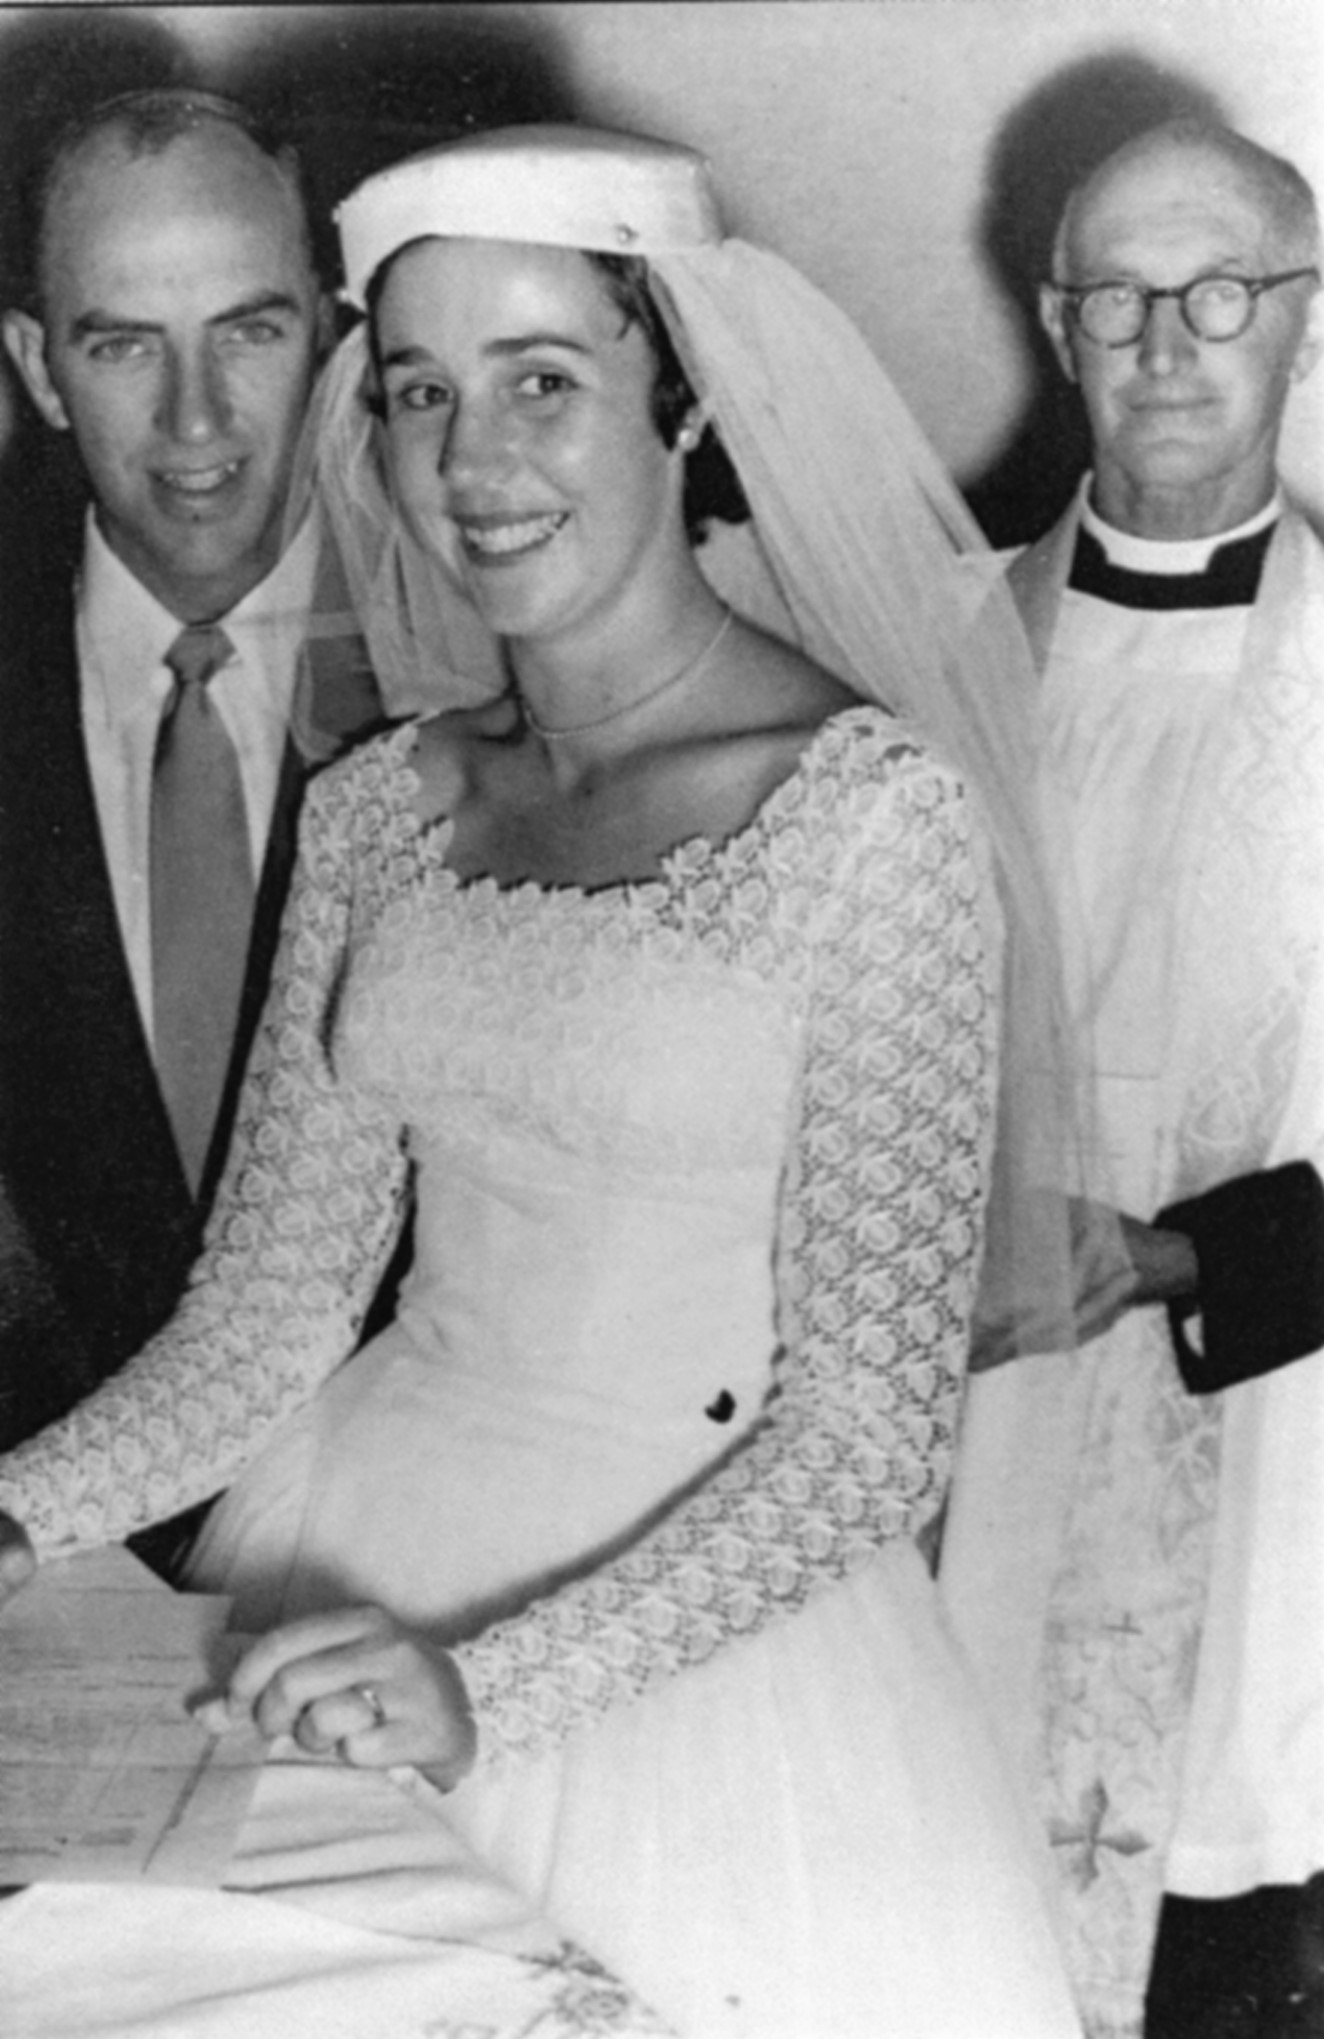
\includegraphics[width=1.\linewidth,center]{../images/Donne.jpg}
\caption{Richard Turner, Janice (McIntosh), Rev R Donne}
\end{center}
\end{figure}


In the 1 October 1956 \emph{Church Chronicle's `}Kilkivan and Murgon' article parishioners gratefully recognized the move from Portland on the far south-west coast of Victoria was a big one for the couple to make. The rector then continued the writings by expressing appreciation for `the warm welcome and much help and kindness from parishioners in every centre' and his `outstanding impressions' of the `loyalty and faithfulness with which Church officers, Ladies' Guilds, Sunday School Teachers and others' had continued in the interim. \footnote{1 October 1956 \emph{Church Chronicle}} These `others' are named in the register of services throughout the first half of the year and into August with the bulk of these conducted by the ever- faithful, retired priest, Rev C Tunstall. Mr S James, conducted a Good Friday (March) evensong in Murgon.\footnote{Parish of Kilkivan Service Register}

After one and a half months of regular services the Venerable Harold John Richards (Archdeacon of Wide Bay and Burnett, 1956-1970) conducted Rev Donne's much anticipated Installation and Induction on Tuesday 25 September 1956 where 120 delighted parishioners gathered in support. Rev Richards was supported in the eucharistic service by Rev Robert Mawson, rector of St Peter's Gympie and rural dean of Wide Bay from 1955 and Rev Reuben Athelstance Foote, rector of St Michael and All Angel's, Kingaroy. A collection to support the Mission to Seamen was noted on 21 October with a congregation of 33.\footnote{1959 Diocesan Year Book} It is around this time that the names of N A Greenbury, G C Quinn, and L Sempf were registered in the Diocesan year book as wardens of the parish.

Although attendance at services had remained at a reasonable, though slightly lower level, with some centres receiving somewhat intermittent and irregular attention for some time, parish finances had once more taken a down-turn. The surge in congregation numbers now evident throughout the parish brought with it a renewed desire to attend to the current low financial position and then to formulate a better budgeting system based on a system of pledged giving.

Throughout 1956-1957 the Murgon Ladies Guild continued to `step-up to the plate' catering for function ranging from Film Nights, through Football Club dinners, tractor displays, the rector's induction service refreshment plus many weddings, not to mention the ever-present street stalls and the efforts of individuals such as the diligent Mr and Mrs Gedge with the sale of produce, fresh and preserved, from their extensive gardening efforts. As a result, their efforts covered several large expenses such as a payment of \pounds600 to the State Electricity Commission, the installation of an electric light over the church gate, donations to Red Cross and Church Missions, the local Church of England Youth Club and the Sunday School, as well as financing the ongoing, mundane needs for brooms, `Brasso', furniture polish and so on. In addition, the parish general fund (referred to as Warden's Fund) was augmented.\footnote{Murgon Ladies Guild cash book (1940-1966)} However, the shadow of needed funds hung heavily over the otherwise smoothly running parish and in spite of the gallant efforts of the guilds at all centres and other parish groups' arranged social ventures.

January 1957 heralded in a year of enhanced efforts on many fronts and did nothing to dampen the drive forward with efforts for a parish hall in Murgon and a church building for Windera.

\section{Building Projects 1957}

\subsection{Parish Hall}

The `voiced' desires for a parish hall to be built in Murgon began to take concrete form through several meetings in April where preliminary planning ideas were discussed and a committee was appointed with authority to arrange for plans and specifications to be drawn up. By the end of the month these had been obtained and submitted. It was envisaged that approval be sought and gained in time for `a start at an early date'. Blueprints had been drawn up by the end of July, costing information was being sought, and an imminent start to this `urgently needed' project was envisaged.




\begin{figure*}[!htb]
\begin{center}
\includegraphics[width=1.\textwidth,center]{../images/parishHall.png}
\caption{Christ Church Murgon and Parish Hall}
\end{center}
\end{figure*}


A 25 October 1957 letter confirmed that acceptance of the plans had been `approved and (plans) returned herewith' -- signed `Archbishop'. A contract was let to builder, J W Goodchild, the hall `to include a well-equipped kitchen and a kindergarten room' with plans for the facility to be operational in early 1958.\footnote{\emph{Church Chronicle} articles, 1957: 1 February p 59; 1 April p 122; 1 July p 219; 1 August p 257; 1 December p 380.} Eager to proceed, in October the parish administration team contacted the Diocesan Property office applying for permission to negotiate a Commonwealth Bank overdraft of \pounds2000 `upon security of a guarantee by the Diocese' to help with financing construction and furnishing'. Total cost was estimated at around \pounds3000. Along with the provisos that all necessary paperwork, signed by the rector, parish wardens and Murgon sub-wardens, be submitted and satisfactory reduction amounts be agreed with the bank, permission was granted and subsequently `executed under Diocesan Seal on 18 December 1957.\footnote{Diocesan Council Minutes 31 October and 31 January 1958, Diocesan Archives, Brisbane.} Construction work began and progressed rapidly with an April dedication date in mind.

\subsection{Windera Church}

Dedicated planning again progressed at Windera early in 1957 with a `last day of February' meeting in the then venue for church services, the local public hall. The general design and dimensions were approved and Mr C Noffke assigned `to arrange for scale plans and specifications be prepared. The local guild minutes support the above, also recording a funds balance of \pounds170, for general expenses and support of the guild building fund. July saw the also `urgently needed' Windera project had progressed to the `Blueprint/costing stage with building to be commenced `as soon as Archbishop in Council approval has been received'.

Approval (and return of all plans and blueprints) was conveyed in a letter of 25 October 1957. Great progress continued into December with logs, kindly felled and donated by Mr C Noffke and Mr D G Baulch from their properties, being milled locally to provide the hardwood frame. \footnote{\emph{Church Chronicle} articles, 1957: 1 February p 59; 1 April p 122; 1 July p 219; 1 August p 257; 1 December p 380.} Diocesan permission for a bank overdraft - limit of \pounds500 - was sought for the Windera church's bank account held in the Commonwealth Bank, Murgon. Duly granted, \footnote{Diocesan Council Minutes 31 October and 31 January 1958, Diocesan Archives, Brisbane.} this allowed local builder, Mr Luke Pringle to be engaged to oversee the project assisted by eager local community volunteers -- a `big call' for the local dairying community whose farming commitments included morning and afternoon `milking of the herds' and the growing of fodder for same. Women willingly played their part as well with many and varied task including provision of refreshments and all painting and oiling of timbers left in their competent hands.

From the Windera Guild minutes Rev Donne did not approve of the locally favoured `St Katharine's' and suggest several alternative `English saints'. With the April dedication date drawing nearer Mrs Margaret Donne, whose name appears as a regularly attending guild member, suggested a compromise, not from either party's list. The church of The Holy Spirit, Windera was finally so named allowing appropriate documentation to be completed.

While building projects seemed to take centre stage in 1957, parish business carried on regardless, as indicated by several Murgon's guild cash book where several entries covered events such as street stalls and varied functions catering along with expenses incurred. Mrs Donne is mentioned several times, indicating her willing involvement. Similarly, the services register records events ABM deputation's visit on 9 March where a Miss Thelma Cook addressed the congregation. The blessing of the Simnel Cake is a notation for 16 March (Lent IV) while the 25 April entry introduces IR Sharp as a lay-reader.\footnote{Parish of Kilkivan services register, March 1957, Diocesan Archives, DJ 3 Box 2}

Several Church Chronicle 1957 articles mention further general business items such the Blessing of the Plough ceremony at the Murgon Show, the fact that 20 children were baptised during the month of April, the rector's glee that he `made some needed repairs to the rectory (admittedly) with the help of a more experienced carpenter', with timber generously supplied by C Noffke (Windera) and had installed a complete set of kitchen cupboards, courtesy the parish council. The parish council, on the recommendation of the treasurer, Colin V Lord (Boonara), introduced a `car depreciation fund'.\footnote{\emph{Church Chronicle} 1 May 1957 p. 156}

1958 ushered in some major celebratory events for the two exciting building projects. The brand-new hall hosted the Wednesday 5 March Lenten Eucharist (conducted by the rector) and then blessed at an intercessory service at 7.30 pm that night.\footnote{Parish of Kilkivan Services Register March 1958}

The Venerable Archdeacon Harold John Richards once again graced the parish with his presence in the parish on Sunday (Whitsunday) 25 May 1958, which marked as `very special' day in parish history with two major functions. Firstly, he officiated at the 7.30 am eucharist then conducted the official `Dedication of the Parish Hall' at a 10.00 am before a congregation of 125. A new era of extended activities was heralded in with activities groups joyfully and thankfully receiving the extra space and freedom. The spacious facility with a kitchen area and three other separate areas allowed Sunday School classes to be conducted more comfortably and numbers increased. The Youth Group met in the hall as well under leadership of Mr Norm Carr, a teacher at Murgon High School, with many and varied activities from play-reading sessions to full blown social dances on the lovely crow's ash dance floor.

This was followed by a luncheon. At a 2.30 pm service, with a congregation of 280, the outlying centre of Windera where the equally exciting official dedication of the Church of the Holy Spirit Church took place. Rev Richards was officiant and preacher at each function. The signatures of both Richards and Donne accompanied the register entries.\footnote{Parish of Kilkivan Services Register May 1958}

By 1958 various methods to boost funds and encourage regular giving had received considered and deep investigation. Adding to concerns, a new vehicle was required, the current one having over 60,000 miles `on the clock' needed to be replaced. Permission to apply for an overdraft of \pounds400 was sought on 29 September. Rev Donne favoured the Wells Scheme which had seen successfully applied in several other parishes. However, the fee of \pounds1,400 for obtaining their services was considered too expensive. This proved to be an insurmountable obstacle and a special committee sought further more achievable options and finally adopted the Anglican Promotion Scheme in 1958 and embarked on a promotional \emph{Every Member Canvass} totally organized and conducted by locals of the area. 4 September is marked in the register as `Stewardship Sunday'. The decision was implemented and introduced through special promotional Loyalty Dinners during September 1958 at Kilkivan, Goomeri and Murgon centres, considered to be central for locations. Murgon's function on 16 September was a double celebration with Murgon-born Rev David Shand (Nambour), son of the parish's first vicar (Rev Rupert Warner Shand, 1919-1922) as guest speaker. The 1 November \emph{Church Chronicle} article reported that around \pounds1,200 had been pledged -- `a very satisfactory outcome'.\footnote{\emph{Church Chronicle} 1 Nov 1958 p 148}

During September the parish received a visit from a Church Missionary Society's representative who gave an interesting account of CMS outreach involvement. The following week the work of lay-readers, J Sharpe and E Miller, in conducting a Morning Prayer (Matens) is recognized. Similarly, on 26 October recognition was given to the GFS group through a special Friendship Service and the dedication of their new banner.\footnote{Parish of Kilkivan Services Register September/October 1958}

Rev Donne officially offered his resignation of his licence as Rector of the Parish of Kilkivan to Archbishop Reginald Halse, in a letter dated 28 October 1958 to take effect from 10 November -- duly signed and notated `Accepted to take effect on the above- mentioned date'.\footnote{Diocesan Registry files.} The final entry bearing his signature is shown in the register on 9 November with a 7.30 am eucharist in Murgon with 38 communicants.

The Donnes returned to Victoria. Ronald Alfred Donne died in Portland Victoria. The following entry appears in the Australian Death Index 1787-1985:

Ronald Arthur Donne, Birth: about 1898, Death: Portland, Victoria (registered 1963), Registration Number: 17471\footnote{Diocesan Registry files.}

With no incumbent priest, services during the remainder of 1958 and into August 1959 continued to be faithfully conducted throughout the parish. Rev C Tunstall, who had retired to Murgon with a general licence conducted regular Holy Communion services and lay-readers I Sharpe, E Miller and W Atkins assisted with Matens and Evensong services. Register notations include the Family and Prize Giving service with I Sharpe on 30 November and the 7 December showing of a Jungle Doctor film strip at evensong.

During December the parish officials offered two possible replacement priests, namely Rev M Paxton Hall (Childers) and Rev Frank Knight (Palmwoods). The letter also included concern that no one was available to conduct Christmas Holy Communion Services as Rev Chas Tunstall had made prior plans to be away, along with willingness to accept a Christmas 1 service in lieu. The Murgon service register indicates Matens on Christmas Day followed by a 28 December (Christmas 1) Eucharist with Rev J Tunstall (rector, Wondai/Proston) and the appearance of a one-off 7.30 pm Holy Communion service conducted by Rev M C Richter.

\section{1959 : Rev Derek Barrett}

Diocesan correspondence indicates that in an August 1959 communication dealing mainly with details regarding Rev M Richter, a request that 'in the meantime' the parish `would be very appreciative of the temporary appointment of Rev Derek Barrett as Priest-in-Charge' is added. Rev Barrett was duly appointed as a locum tenens Priest-In-Charge of the Parish of Kilkivan in 1959 following Rev Donne's departure. The Registrar informed the locals that `\ldots while he is (so employed) he is to be paid a stipend'. The minimum annual stipend of \pounds850 pa is mentioned as applicable, in addition to rent-free use of the Rectory.\footnote{Diocesan Correspondence} He signed using his full name in the services register as resident in the position on 9 August 1959. Records indicate he used the initials DB during uninterrupted service in Murgon until 13 December of that year. The Murgon Guild purchased a gift and provided supper for Rev Barrett's party and supplied `groceries for the rectory'.\footnote{Murgon Guild Cash book, Jan 1959-60}

Former Murgon Student Hostel residents for the 1958-1960 period have recollections of his presence at that nearby establishment and a friendship with the Superintendent and Matron, Mr and Mrs John Else and their daughter Enid. Clergy records indicate that he served as assistant curate, St Paul's Maryborough, prior to his 1959 Murgon appointment and similarly at St James Toowoomba (1959-1961), so he was reasonably situated as to allow some occasional travel to Murgon. He spent from 1963 as a priest in the UK until his retirement in 1990, finally returning to Queensland with spouse Gwendolene in 1997 with permission to officiate in Brisbane Diocese.
\balance

\printendnotes[custom]
\setcounter{endnote}{0}
\chapter{1959--1962 : Rev Murray Clifford Richter}
\nobalance




\begin{figure}
\begin{center}
\includegraphics[width=1.\linewidth,center]{../images/richter.png}
\caption{Rev Richter And Family}
\end{center}
\end{figure}


Archival correspondence indicates mounting, though politely phrased, tensions within the parish regarding the prolonged period of interregnum. Positive signs in the Parish Council minutes began appearing in the early months of 1959. Correspondence from the Diocesan Registry files signed by Wardens and Parochial Nominators, E Miller, L Sempf and R Mander-Jones, confirm that negotiations towards the possible appointment of Rev Richter (1924-2011) had begun soon after Rev Donne's notice of relinquishing the rectorship of the parish. A letter to Diocesan Council, dated 18 March 1959, officially nominated Rev Murray Clifford Richter for the position of Rector of the Parish of Kilkivan and urged the council's urgent consideration and acceptance of the nomination, to be followed by a formal Diocesan approach to Rev Richter. Personal reasons of `family ties and schooling for his (three) children' were cited as underlying his desire to come to the Brisbane Diocese.

Subsequently, the 2 June correspondence referred to a visit to the Parish by Rev Richter where he conducted all five services across the parish, there was a strong desire for his appointment and that all `are even more anxious for his appointment\ldots{} and now keenly await the results of the discussions he is having with his Bishop'. It appears Kilkivan's enthusiasm for this move was not so enthusiastically shared as discussions between the Brisbane and Armidale Diocese indicate. A letter from the Diocesan Registrar to Kilkivan's parish wardens, states in part `\ldots I believe the Archbishop of Armidale does not consider that the clergyman has sufficient experience to accept the position in your parish...'.

Never-the-less Kilkivan area was firm in its resolve and pressed on stating that as Rev Richter had apparently met with diocesan officials in Brisbane, they `\ldots felt sure that having met our nominee you will understand our strong desire to have his services in our Parish'. Their application to have Richter appointed was formalized in minutes of 25 July 1959 on a motion by Mr Sing and seconded by GC Quinn. There followed an August letter, again signed by Miller, Sempf and Mander-Jones stating that they now `had ascertained' that `the Bishop of Armidale was willing to release him (Richter) at Christmas time'. To prevent further delay they were requesting `urgent placement of the nomination before the Presentation Board'. They further requested the Board support them through affirmation forwarded to the Bishop of Armidale along with a request for Rev Richter's release as early as possible in December to allow settling in time prior to Christmas. Responses to each of the parish's letters were duly received.\footnote{Diocesan Correspondence Files, 18 March, 02 June, 25 July, 28 August 1959)}




\begin{figure}
\begin{center}
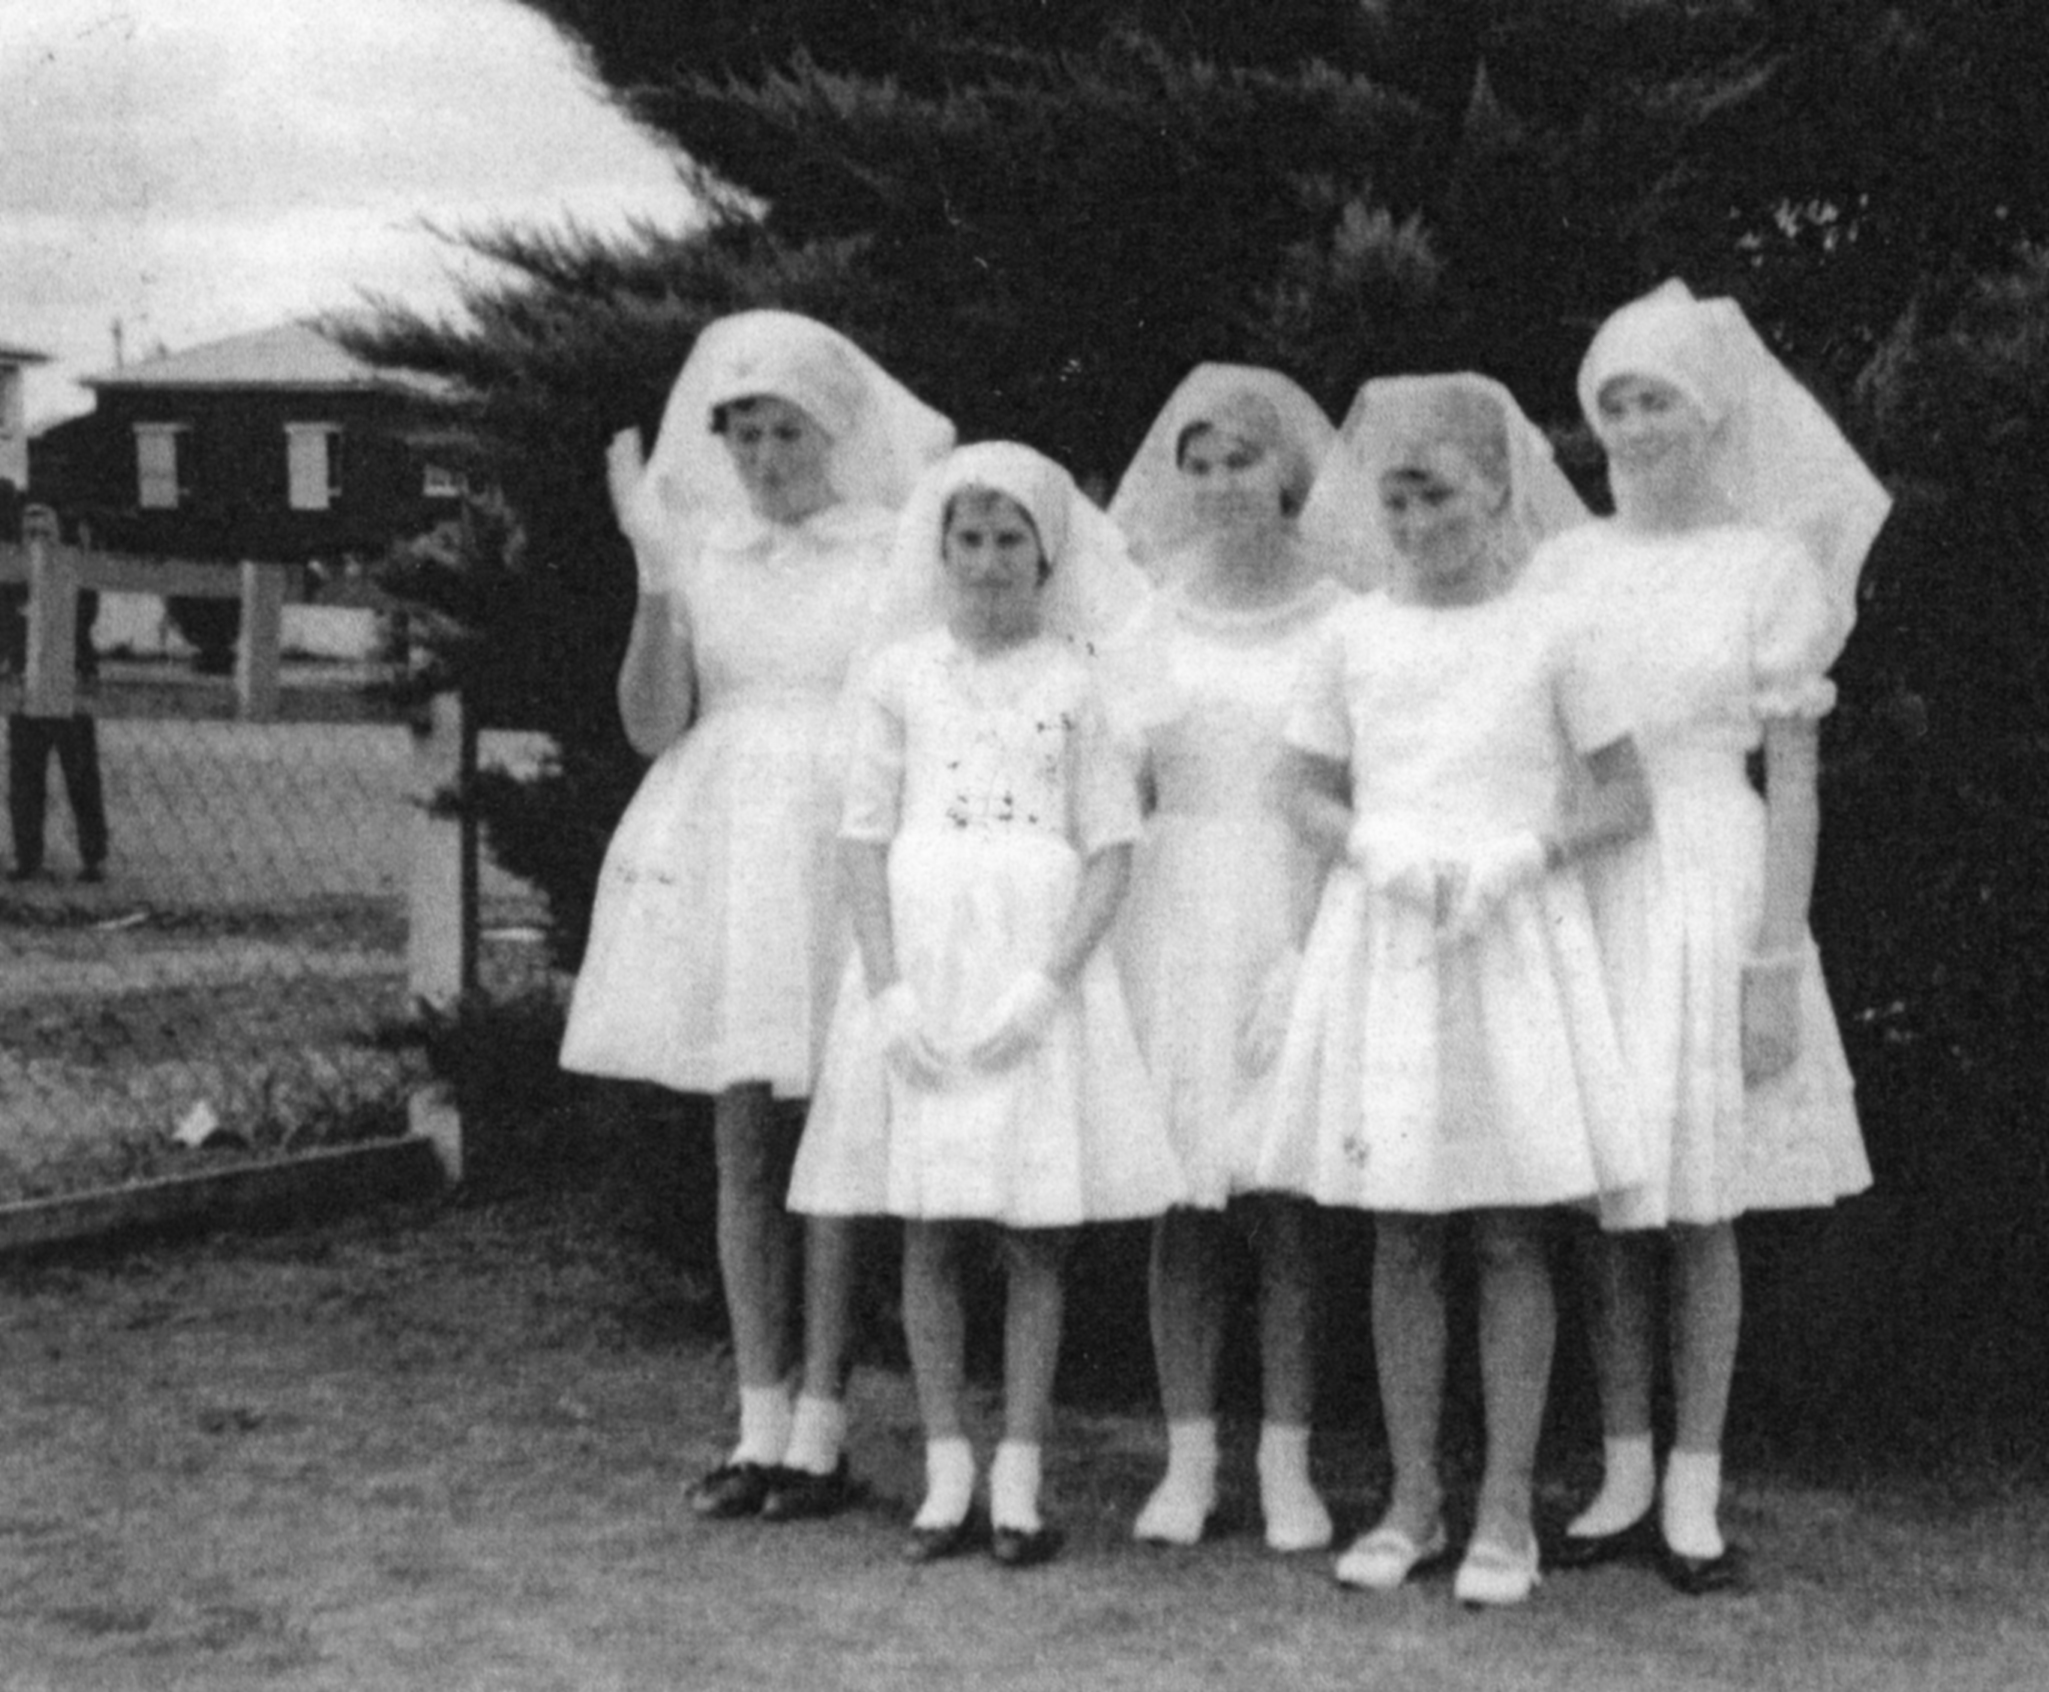
\includegraphics[width=1.\linewidth,center]{../images/confirmation1962.jpg}
\caption{Confirmation group, Murgon, 1962}
\end{center}
\end{figure}


The Parish Council minutes of 1959 reveal that all ongoing business, as well as the necessary preliminary arrangements for the new rector's arrival, was attended to. This included the wind-up of short-term rectory rental agreements, a \pounds50 donation to Rev C Tunstall in appreciation for services to the parish and the proposal of \nicefrac{1}{2} fares for a taxi for Mr Atkins to continue providing lay ministry to Cherbourg to be arranged. A `Parish Canvass' to boost depleted funds to be organized.

Entries from an accompanying water-stained services register indicate regular 2\textsuperscript{nd} and 4\textsuperscript{th}Sunday services at alternating 11.00 am/2.00 pm time slots on a month-about basis from 27 December 1959 through to 27 January 1963. No mention is made of the venue though on these pages, although mention of a baptism for Donald George McAntee (14 February 1960 @ 2.00 pm) leads to the conclusion that it is part of a similar earlier find by former Diocesan Archivist, Glenda Murrell, and that it is from the Windera church. The McAntee family were, over three generations, resident in Windera and church members there for many years. Local knowledge indicates a similar pattern 2\textsuperscript{nd} and 4\textsuperscript{th} Sunday services was in place at St David's, Boonara with the order of times reversed. Rev Richter continued to follow the parish custom of five services per Sunday with variations to include 11.00 am and 7.30 pm at Goomeri and Kilkivan and to cater for Holy Communions at Cherbourg.




\begin{figure}
\begin{center}
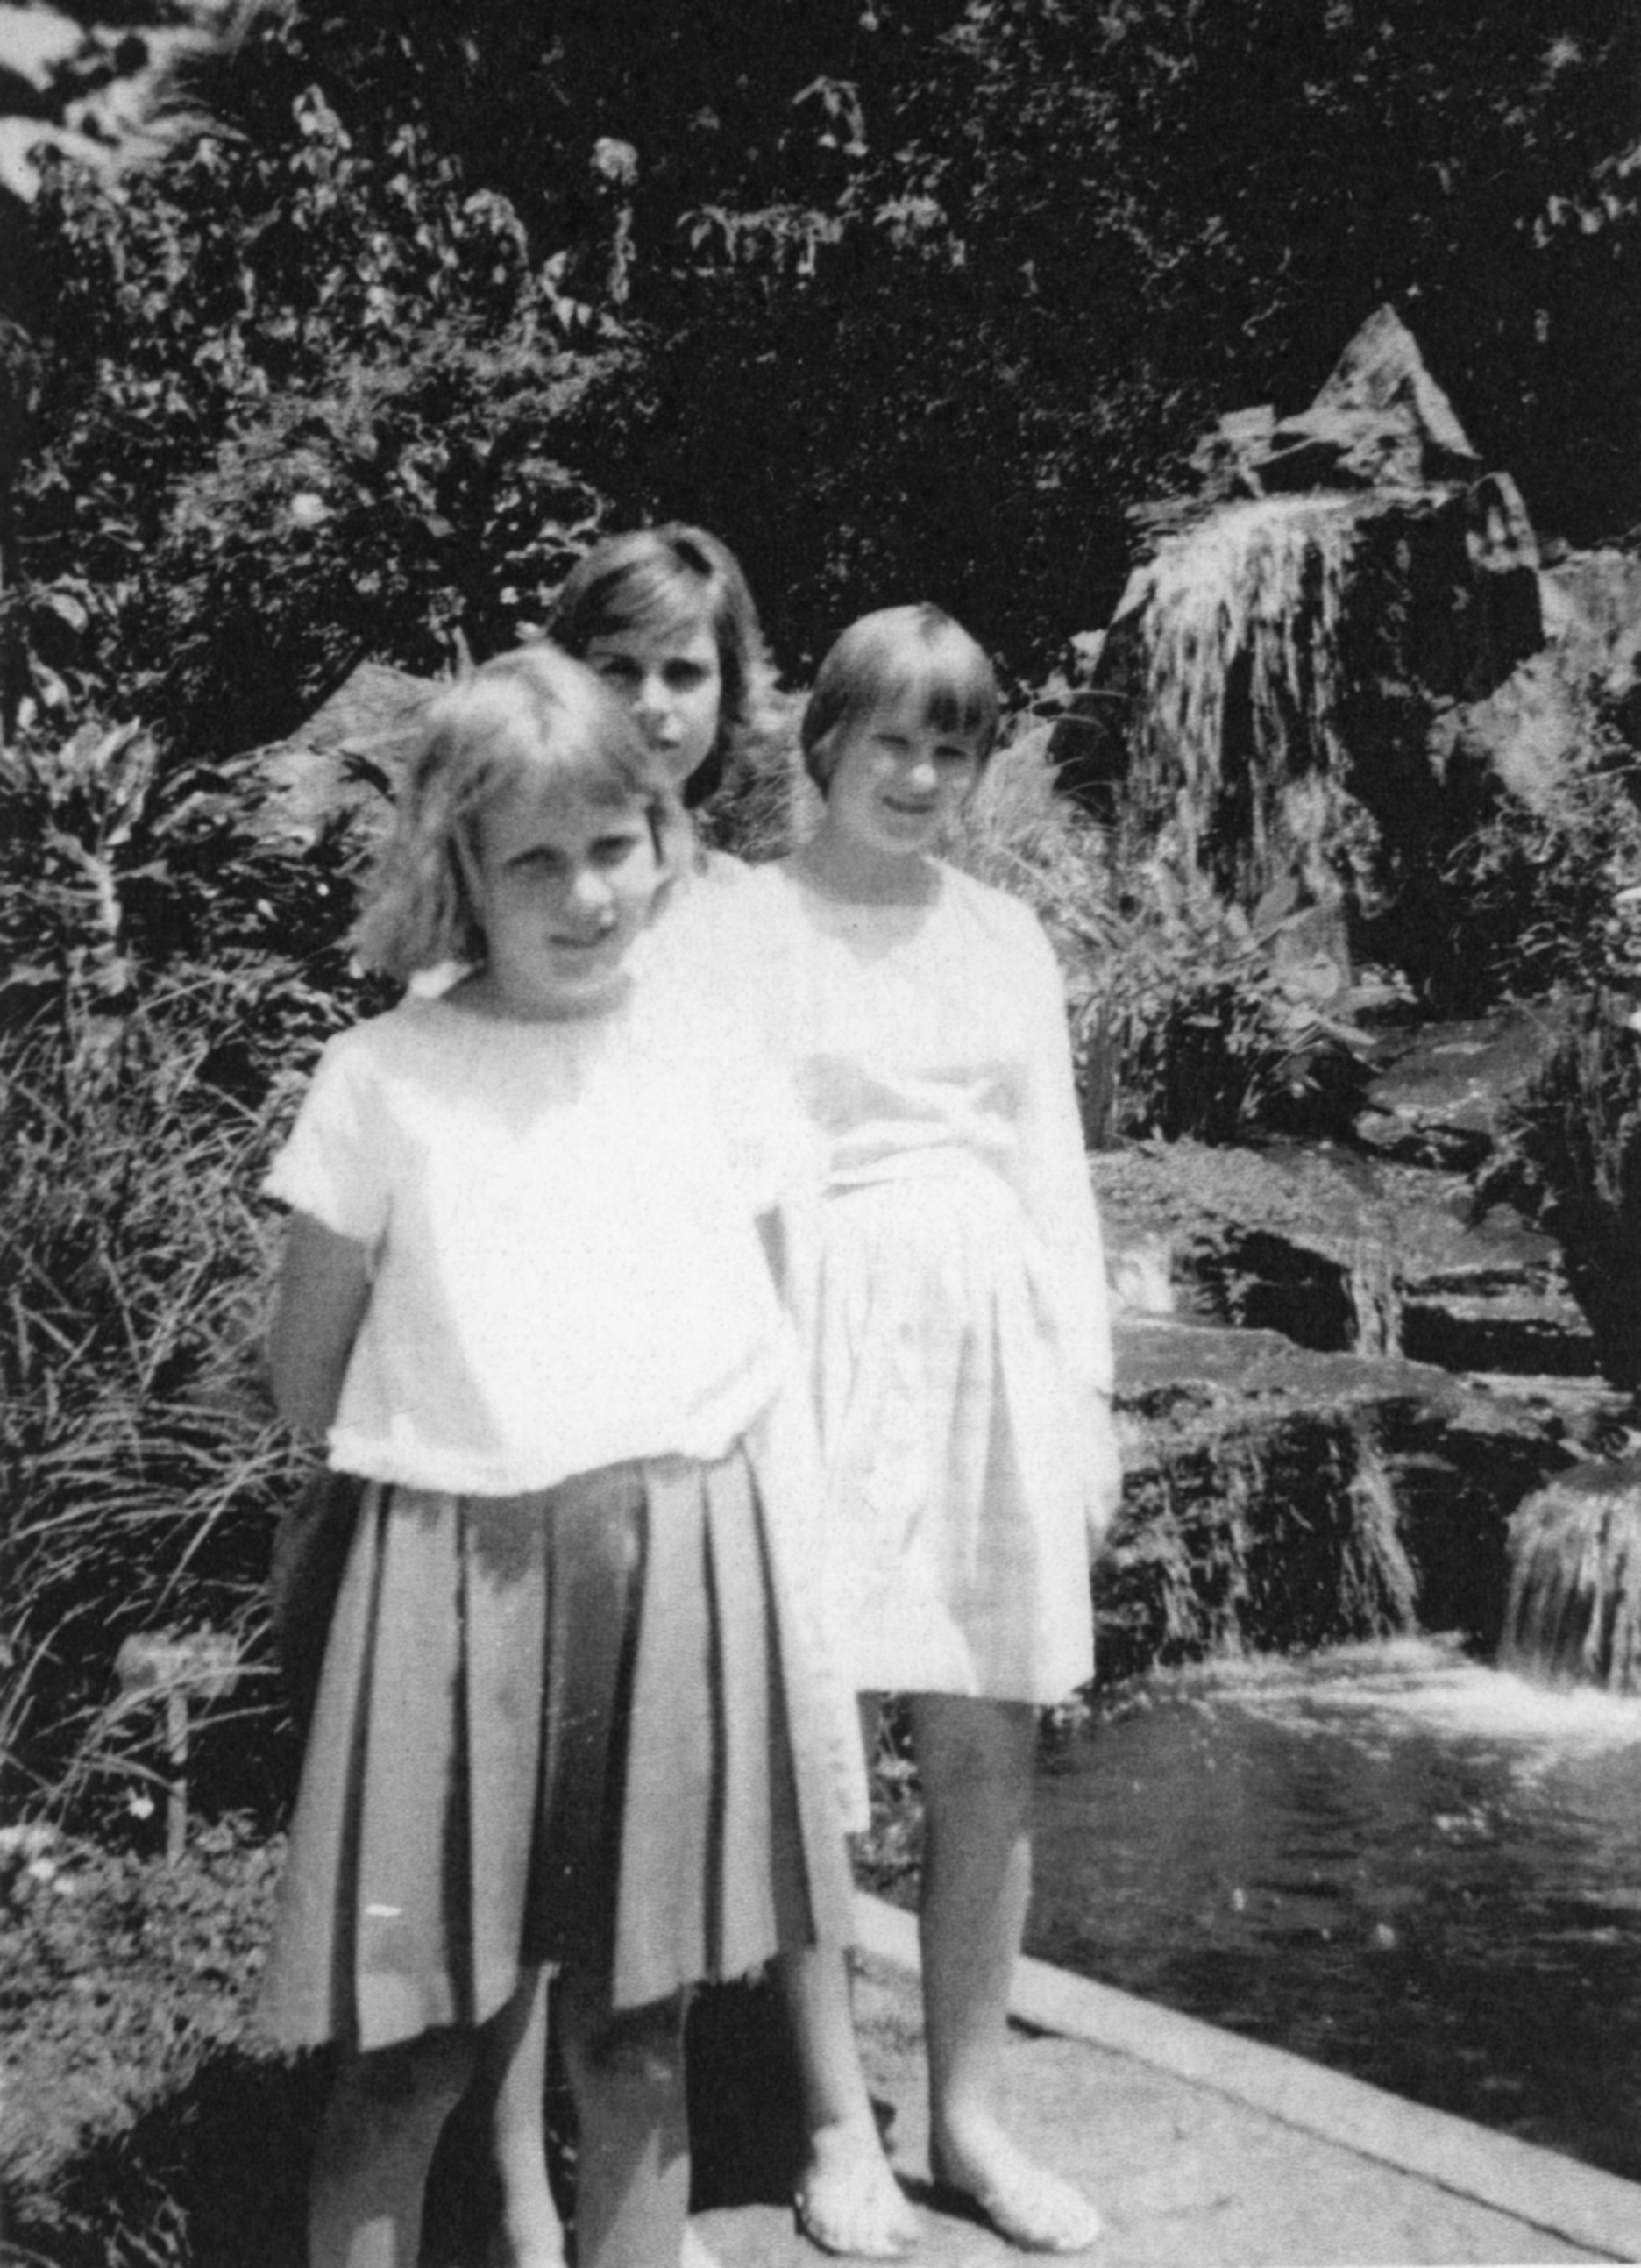
\includegraphics[width=1.\linewidth,center]{../images/gfsBrisbaneTrip.jpg}
\caption{GFS Brisbane Trip}
\end{center}
\end{figure}


For over a year (10 November 1958 - 20 December 1959) the Kilkivan parish had been without the services of a full-time presiding priest. Though exceedingly grateful for the combined efforts of volunteers and the one month's locum-tenens service of Rev Derek Barrett, which had kept the churches in all centres at least `ticking-over', the arrival of Rev Murray Richter was greeted with joyous relief. He and family came to Murgon from the township of Baradine situated northern inland region of the Diocese of Armidale, northern NSW, on a stipend of \pounds975/pa plus house and car (a late 1958 model Holden) with all motoring expenses paid. Diocesan files record that on 16 December 1959 `\emph{The Rev Murray Clifford Richter was this day licenced as Rector of the parish of Kilkivan effective\ldots'} as from date of writing.\footnote{Hand-written Diocesan Register of Appointments, p. 34 (665)} He conducted his first service in the parish on 20 December, 1959, one week after Rev Barrett's departure.\footnote{Diocesan Correspondence File.}

The 1 February 1960 Parish Council meeting announced that, after 24 years of paying rent to the Murgon centre, (totalling \pounds936 for the term) responsibility for the Rectory was, finally, to be taken over by the Parish of Kilkivan. It was noted that the property was badly in need of attention. Urgent initial repairs were to cost \pounds308 with painting costing \pounds211. A total of \pounds176 was still owing on the car account. Ideas for procuring interest free loans were discussed. A letter conveying this was forwarded by R Mander Jones to the Diocesan Registrar. By 6 April approval was received along with due consideration for repayments.




\begin{figure}
\begin{center}
\includegraphics[width=1.\linewidth,center]{../images/rectoryRepairCost1960.png}
\caption{Details of repairs}
\end{center}
\end{figure}


With the new rector's arrival, it became glaring clear that urgent attention was required in many areas, especially `to get the parish back on its feet'. Though clearly and appreciatively acknowledging the efforts of the dedicated and generous efforts which had kept the parish functioning smoothly with regular worship, it was obvious the work-loads had had an effect on morale. At the conclusion of this first Parish Council meeting under Rev Richter's chairmanship, where a review of the preceding year's events and future plans were discussed, wardens Miller and Sempf, parochial nominator R Mander-Jones and honorary secretary/treasurer C V Lord `felt compelled to write' to the registrar Mr St Johns offering thanks for his `assistance, approachability, and sound, down-to-earth advice' during the period without a rector.

The new page in Murgon's history brought with it an immediate surge in vitality and energies as evidenced in the minutes of the first Parish Council meeting chaired by Rev Richter in February 1960, and continuing throughout an action-packed first year. The main items dealt with included immediate attention to a new tank for the rectory; urgent repairs to pot-holes in the driveway; a much needed extensions to St Matthew's Kilkivan; and the printing of a Parish Paper.

All centres were urged to address `assessments in abeyance' by 31 May 1960 and several urgent items were addressed including the purchase of a filing cabinet and cards for the church office; Letter Heads for correspondence; and the installation of a `moveable phone' and three extra power points. It was proposed to purchase `a full set of vestments for priests' use, to remain property of the parish.

The completion of a full set of Centre Rolls and a full Parish Roll was addressed by the meeting. The mooted and earlier attempts at a `Parish Canvass' were to be fully implemented in order to formalize pledges for budgeting purposes.

The meeting also voiced ideas to assist Goomeri centre where Sunday School for 66 children was currently attempting to operate in a church to hold 40 people and discussed an approach to Diocesan authorities `to help eliminate the problem of parishes enduring long periods without a priest', suggesting the possibility of enforcing `a limit to the waiting-time'.

It is pleasing to note the appearance, alongside the now familiar long-servers, of `new names' in the records (C V Lord, F Narracott, G Sturgess, D McIntosh, D Kay to name just a few) who actively contributed in many and varied roles.

A concerted effort to provide more assistance to the parish for work in Cherbourg was brought to the notice of the general parish community by lay reader W Atkins and Cherbourg Superintendent, Mr Sturgess who was also a parish warden. A motion to be presented to the Diocesan Synod requested that there be a discussion on `\ldots{}\emph{the general conditions existing in Cherbourg in relation to Religious Instruction and to whether a part-time curate could be employed, sharing the balance of his time in the parish of Kilkivan'} together with a query re Diocesan assistance being given. The rector and wardens were empowered to further investigate `Cherbourg and Home Missions'.\footnote{Minutes 2 Feb to 6 September 1960}

The progressive spirit was evident throughout the parish. St David's, Boonara pushed ahead with its plans for alterations to enlarge the church and applied of a bank overdraft limit up to \pounds700 which came into effect in August 1960.

Rev Richter, a qualified architect `drew up the plans' for St Matthew's, Kilkivan's extensions which were dedicated on `25 September 1960 with the Rural Dean, Rev R D Turner, officiating'.\footnote{Kilkivan Centenary Book pp 15/16} However However, the cost remained to be paid and by 30 October 1960 the application for an increased bank overdraft for St Matthew's centre, authorised by the rector and parish wardens Messrs Sempf, Miller and Pearson, had been approved by the Diocesan Properties Board.

From the Diocesan end came a proposal for an alteration to the Kilkivan parish's boundaries to allow the Manumbar Mill centre to become part of the Nanango parish `as the Nanango rector would be more able to provide the ministry it deserves'. Fully supported by all parties, the proposal became fact in 1961.\footnote{Diocesan correspondence 30 December 1960 and 4 August 1961}

\section{The New Rectory}

The condition of the rectory premises and the expense required to complete the ever-mounting repair and maintenance requirements, along with its distance from the church, led very quickly to suggestions of its sale and the purchase of a more suitable dwelling for a family. Application was made through the Diocesan Registrar for permission to proceed along these lines as an attractive brick house in Watt Street adjacent to the church had come onto the market. Diocesan Council responded with `sympathetic consideration \ldots{} when they (the parish) are in a position to submit a definite proposal' regarding details of overdraft required `to finance the difference between the sale of the present rectory and the purchase price'.\footnote{Minutes of Diocesan Finance and Property Board 17 April 1958 -- 13 July 1961.} However, this proposed purchase did not eventuate.




\begin{figure*}[!htb]
\begin{center}
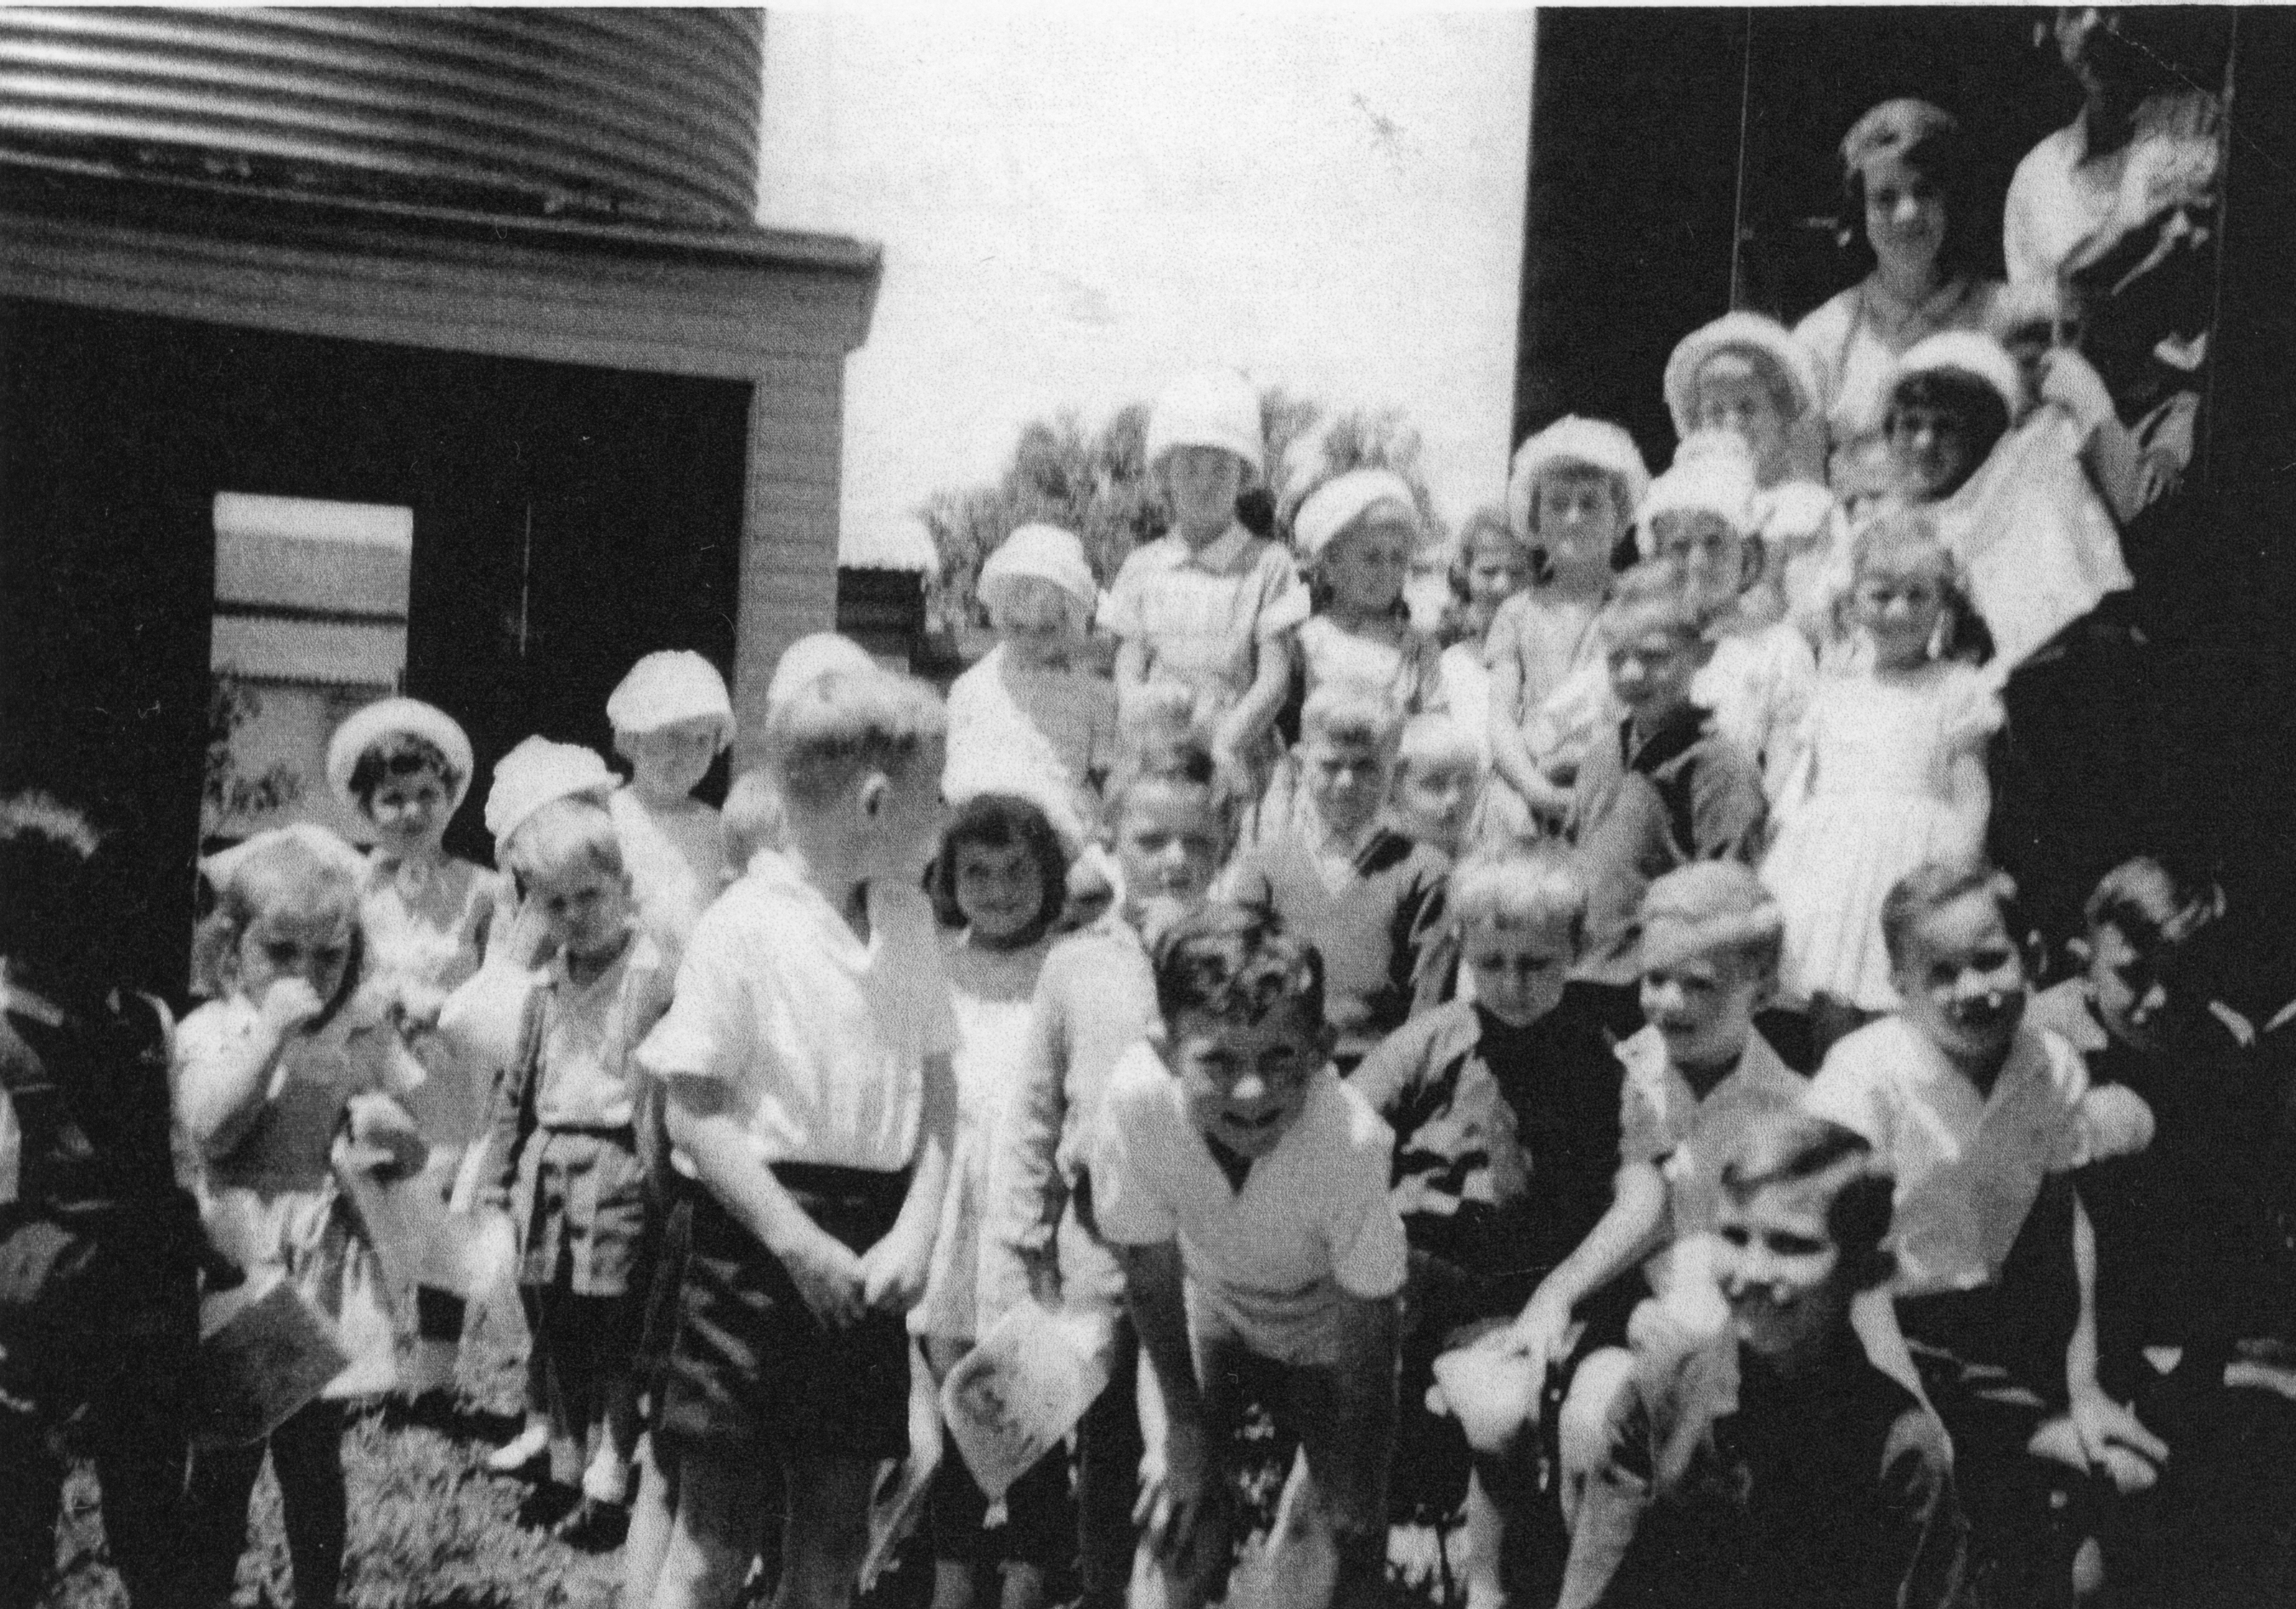
\includegraphics[width=1.\textwidth,center]{../images/sundaySchoolChildren.jpg}
\caption{Children at Sunday School}
\end{center}
\end{figure*}


The November 1960 parish minutes began on a solemn note with a minute's silence as a mark of respect for parish member, Mr Les Eland, killed in a tragic accident -- a fall from a hayshed roof while assisting a neighbour and fellow Boonara parishioner with repairs. A letter of sympathy was forward to his widow, Jean. A bell and bell tower in his honour was later added to St David's Church. Jean Eland continued uninterrupted service to the church until her passing at age 80 in 199?? Her bequest to Boonara centre was utilized on renovations to the front porch and the purchase of a portable home communion case for parish use -- both dedicated to her memory.

The mood of the meeting lifted with the news that the long-mooted desire for a new Parish Rectory in Murgon had finally begun to take shape, with Mr Miller outlining the outcomes of the warden's meeting. Much discussion and sharing of wide-ranging views led to a motion move by Mr Frank Narracott and seconded by Mr Ogg `that the wardens go into the matter of a new rectory; that plans, costs, finance and disposal of old rectory' be investigated. Much effort and expense had already been expended on the old and deteriorated rectory and with further expenses considered to be around \pounds300 just to have it considered safe as a place of habitation while still not up to requirements, disposal and new-build seemed sensible way forward.\footnote{Parish council minutes 28 November 1960}

A qualified architect, Rev Richter immediately began working on the design and plans for the rectory and offered to oversee the building process. By mid-December these plans and scale drawings and elevations of the new-build, adjacent to the church, had been completed. Along with the included possible extensions to Christ Church itself plus the size and positioning of all existing buildings the documentation had been submitted to the Murgon Shire Council and `had met with the Shire Engineer's approval'. This information was confirmed in recent communications with South Burnett Regional Council's representative, (Mr Russell Springhall. SBRC holds all documents from the former Murgon Shire records in both original (pencil drawn) and digital form. Details include approval date of plans as 29 December 1960 and builder, Mr Luke Pringle of Garrick Street Murgon. Exterior walls were to be in chamfer boards with the interior lined with Bernie/Masonite board.

A full cost of \pounds4,000 was estimated with an expected \pounds2,000 from the sale of rectory cottage to be utilized immediately in reduction. A qualified builder (Mr L Pringle) had volunteered to be in overall charge of construction, with further builders, joiners, plumber and electrician, all being congregation members and offering service at virtually `price of goods' rates, it was thought that even allowing for small costings margin, the estimate of \pounds4,000 remained generously above requirements. Negotiations for a loan through the lending department of the Commonwealth Savings Bank of Australia were in train. It was hoped Diocesan approval would be viewed positively and processed immediately.

Following receipt of a 20 February letter from the bank (as above) stating its agreement to the requested loan on the basis of a deposit of the deeds and fire policies to both present and new lands and repayment of at least \pounds100 per half year plus interest and an immediate reduction of \pounds2,000 upon sale of present rectory. The relevant Diocesan department expressed concurrence in these arrangements.\footnote{Diocesan Property and Finance Board minutes 23 Feb 1961}

As often happens, the estimated costings fell considerably short of requirements. A 5 July letter from the Rector and Wardens to Diocesan authorities advised of the parish's decision to accept and offer of \pounds1750 from Mr Patrick Joseph Mulhall, Railway Department, Clifton, who was to take possession of the property as from 22 August 1961, pending final payment.\footnote{Diocesan Correspondence} The Diocesan Property Board expressed concurrence, and was asked to proceed with the transfer on the parish's behalf through local solicitor, G B Roberts. The 31 August minutes contained details of transfer as requested, under Diocesan Seal, of Allotment 15, Section 5, County Fitzroy, Parish and Town of Murgon.\footnote{Minutes of D Property and Finance Board, July 1961 -- 9 April 1964}

Although the sale of the old rectory and the transfer of the deeds to Mr Mulhall brought some financial relief, overdraft increases began to present themselves as being necessary evils. By October, the parish treasurer, Mr Colin Lord, telephoned the Registrar stating that a further loan was required for the erection of the rectory now seen to be costing much more than first thought with \pounds5,900 already spent against the original estimate of \pounds4,000 -- the lower sale price of former rectory contribution somewhat to this. The parish expected they could reduce this proposed extra loan of \pounds4,300 by \pounds500 per annum. However, by 11 December 1961, an additional loan of \pounds1,000 was sought `to pay outstanding accounts in connection with the new rectory', bringing the principal overdraft debt to \pounds3,332 with the new loan on top of that. It was recommended that insurance on the new building be increased because of growing costs. In spite of this, spirits remained high and optimism prevailed, with the original concept of being debt-clear in ten years remaining the main aim. The Property and Finance Board's 26 October meeting `felt it necessary to give permission to pay the debts', reluctantly agreeing to increasing the proposed loan to \pounds4,300, along with stated concern for these ever-increasing costs and a requirement for firm commitment to debt reduction.\footnote{Diocesan Property and Finance Board Minutes 27 July 1961 -- 9 April 1964}

Meanwhile, in June 1961 the Murgon centre applied, in a letter through the Rector, for a loan of \pounds500 through the Commercial Bank of Australia to purchase `an urgently needed new Kingsman Duchess Organ'. Permission was granted under Diocesan Seal (27 September) for a loan of \pounds350 against the account, Murgon Church's Organ Account, subject to the usual conditions of formal application and a satisfactory repayment schedule duly attended to as required, with a faculty being granted `under Diocesan Seal' dated 27 September 1961. The Ladies' Guild again stepped up, raising a substantial amount of the purchase price plus the supply of `Hymn books plus freight for the Organ'.\footnote{Murgon Ladies Guild Cash Book entries 1960-1962}

By 17 October 1962 the concerned parish treasurer, Mr Colin V Lord, was strongly advocating a determined Parish Drive for donations to attend to the ever-growing rectory debt.




\begin{figure*}[!htb]
\begin{center}
\includegraphics[width=1.\textwidth,center]{../images/DonMcCleodNormaHutchenson1960.jpg}
\caption{Miss Norma Hutchinson \& Mr Donald McLeod}
\end{center}
\end{figure*}


Throughout his time as rector the further sacraments of marriage and baptism plus funeral duties were diligently and warmly conducted by the rector. To illustrate, in March 1960 the \emph{South Burnett Times} carried a report of the marriage of Miss Norma Hutchinson to Mr Donald McLeod in Christ Church Anglican church which was described as `one of the prettiest weddings seen at Murgon for many years' and continues to describe the bride's entry into the foyer of church to `organist Dr Monz playing a fanfare followed by the bridal march as she, on the arm of her father, entered the church'. In a recent letter, Mrs McLeod, the organist's former practice receptionist states `\emph{I will never for forget Dr Bernard Monz. He asked if he could play the organ. Boy did I say yes quickly. It was beautiful. Felt like we were bringing a whole orchestra with us.'} The article continues with full details of attendants and descriptions of the bride's and bridesmaids' gowns, making special mention of Dr Monz's daughter, Julie, `who made a beautiful little flower girl'.

On the back of this next photo, Mrs McLeod has written \emph{`Don and I were given a surprise by my young Cubs. I never dreamed this would happen. I was `Kim' to them. Noel, my youngest brother actually kept this secret. It was a lovely feeling when I saw them here. They were a good `pack'. Mrs Nichols must have organized it} \emph{all.'}

On 7 July 1961 Rev Richter and churchwardens R B Jeffries and Bernard A Gedge filed a Notice of Intention to apply for a Faculty authorising them `to place a Processional Cross in Christ Church, Murgon, in memory of Dr Bernard Monz. The processional cross is to be used for ceremonial purposes within the church and parish' -- duly signed and dated by the rector and wardens who also advised that due Public Notice `has been attached to the church door for 14 consecutive days' as required. The Faculty was granted as requested on 11 July, 1961 and now forms part of the worship framework in Christ Church.\footnote{.Diocesan Property and Finance Board minutes of 11 July etc.}

An affiliation with Mothers' Union Australia and a group was formed in Murgon with Mrs Dorothy Richter as its first president\footnote{Information courtesy Shirley Waldock.}. Murgon Ladies Guild remained an active and valued support group for all parish activities.

The Kilkivan Centenary book states that `due to his wife's ill health Mr Richter was forced to return to the south in 1962. On 21 August 1962 Rev Richter officially tendered his resignation from the parish, effective 19 November 1962. Official confirmation in a letter to warden, C V Lord, was issued by the Diocesan Registrar along with the necessary forms -- duly completed by parish officials.

From Kilkivan parish Rev Richters returned south to Epping/Thomastown 1962/1969; Frankston E 1969-1971; Chaplain AMF 1970 -1974; Chaplain Brighton GS 1974-1988. Retired 1988 with PTO Melbourne. (Clergy Records

During the interregnum local lay persons conducted services or Morning and Evening Prayer with the occasional assistance (as shown in the December 1962 parish services register for Boonara which also indicates one service - `interrupted -- hail'.) of Deacon Fred Ailwood (later the Venerable Frederick Charles Ailwood) who was active in the area, possibly stationed at either Wondai or Kingaroy. The Christmas Eucharist was conducted by a visiting priest on 23 December 1963. Other occasional sacramental services were conducted by Rev James Anthony Carpenter Shaw who was incumbent in Wondai/Proston parish 1961/1962 and whom the Kilkivan parish\footnote{13 August 1962 correspondence} had nominated as a possible rector to replace Richter, though this did not eventuate. His signature appears for the last time in the services register as officiant at the McIntosh/Stephens wedding on 9 Feb 1963.
\balance

\printendnotes[custom]
\setcounter{endnote}{0}
\chapter{1963--1973 : Rev Alfred John Gerlach}
\nobalance

Rev Alfred John Gerlach with his wife Shirley and three young children, Edwin, Judith and Michael, came to the parish early in March 1963. Murgon, and indeed the entire parish of Kilkivan was blessed with the services of a very intelligent and well-educated man who had completed High School aged just 16, then studied industrial chemistry and developed many and varied practical `Handyman' skills ranging from Crystal radio set making through motor vehicle maintenance to (later on) adding a ground-floor room to the Rectory to accommodate his father. Those who got to know him well have reported a compassionate and understanding `man of the people', and `a deep thinker who could sometimes appear \emph{a little vague} as, lost in thought; he could walk right past a parishioner in the street without a glance'.




\begin{figure*}[!htb]
\begin{center}
\includegraphics[width=1.\textwidth,center]{../images/gerlach.png}
\caption{Rev A Gerlach And Altar Boys}
\end{center}
\end{figure*}


A young Alf Gerlach joined his local Sydney church's youth group. A passage from Ezekiel, encountered during a Bible Study session was his call to a faith which grew and deepened through the years. Born in 1924, Alfred John Gerlach studied for the priesthood through Moore College from 1947, made a Deacon and then Priested in 1950. City born, he served as Curate at Eastwood, 1950-51 and Cammeray, 1951-52, only learning to drive a car when he received his posting as Vicar of the rural northern NSW parish of Wyan / Rappville (1952-58). A promotion in rank led to his appointment as Rector to Bellingen (1958-63). His move to the Parish of Kilkivan began the `Queenslander' chapter which lasted till his passing in November 2019.\footnote{Clergy Notes}

From a 15 March 1963 hand-written entry in Archbishop Strong's personal register of events, `The Reverend Alfred John Gerlach was this day licenced as Rector of the Parish of Kilkivan as from 12 March 1963.' Services began in earnest on 17 March, the first Sunday after their arrival. The stipend at this time was listed a \pounds1,200/pa plus rectory, vehicle and all running expenses.




\begin{figure}
\begin{center}
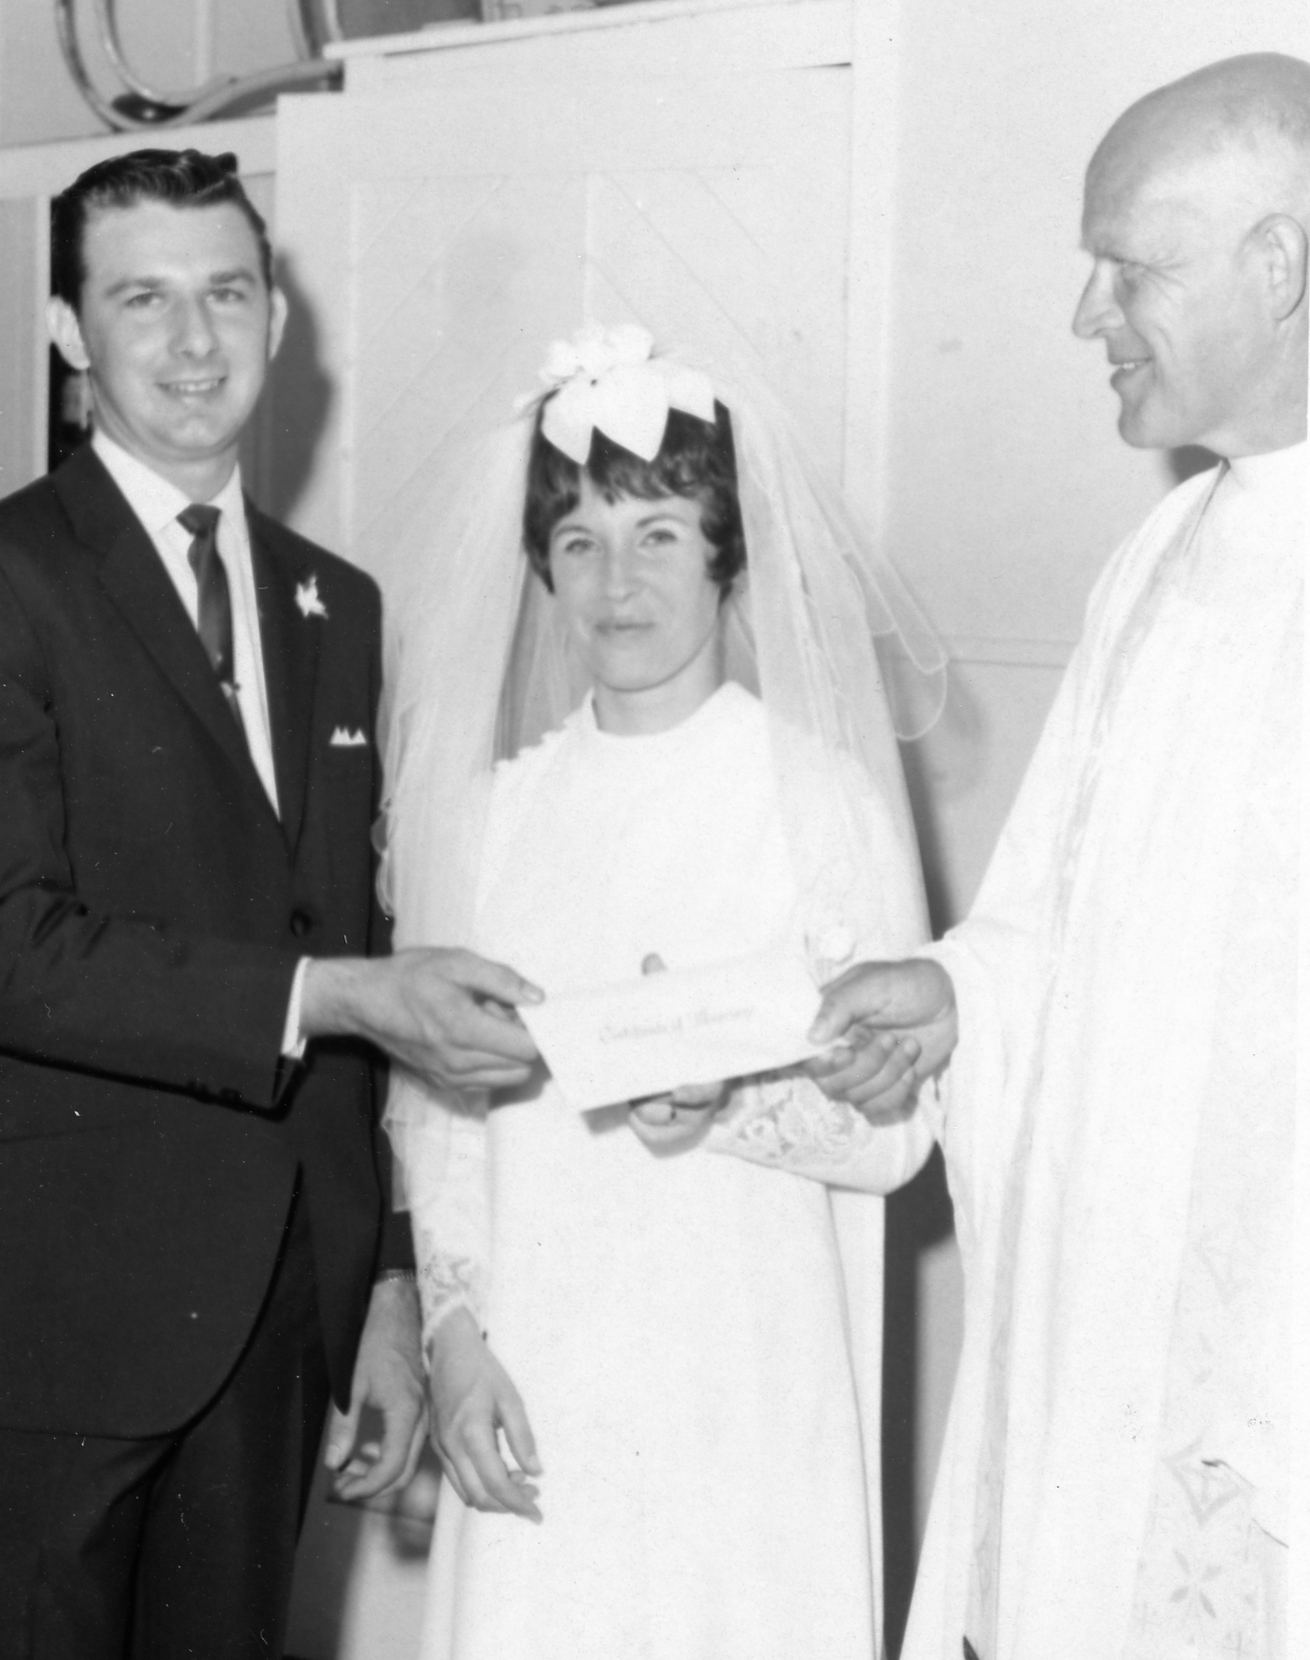
\includegraphics[width=1.\linewidth,center]{../images/lyndaTilneyVestry.jpg}
\caption{Charlie Steele, Lynda (Tilney) and Rev A Gerlach}
\end{center}
\end{figure}


The Gerlach family came to a parish with a positive attitude and into a bright, new, two-storied, five bedroomed Rectory, located right beside the Murgon Church and with a large, well equipped hall to the rear. Buildings in all other centres were in first class order. All services were well attended and numbers attending continued to increase under Rev Gerlach's ministry. A regular monthly pattern of services throughout the parish was developed with up to six services in a day, five of which were conducted by the rector, for at least the second and fourth Sundays each month, along with additional mid-week offices. Groups such as Guilds, Mothers Union, Sunday Schools, GFS, Boys Brigade and Youth Groups were evident in most centres.

The 1963 Year Book records weekly communicants at 185 with 82 baptisms and 9 marriages for the year, along with 17 Sunday School teachers across the centres instructing 219 enrolled children. 16 schools were visited and 4 regular Religious Instructions teachers were actively involved. During his `settling-in' period the support of wardens, Sempf and Lord plus the Kapernicks and Mr Gedge in particular was much valued. The Gerlach children were readily accepted into all community activities and many enduring family friendships were cemented. Rev Gerlach, a tall man, quickly became well-known for his long strides to the organ whilst still singing loudly if no organist was available at a service.




\begin{figure}
\begin{center}
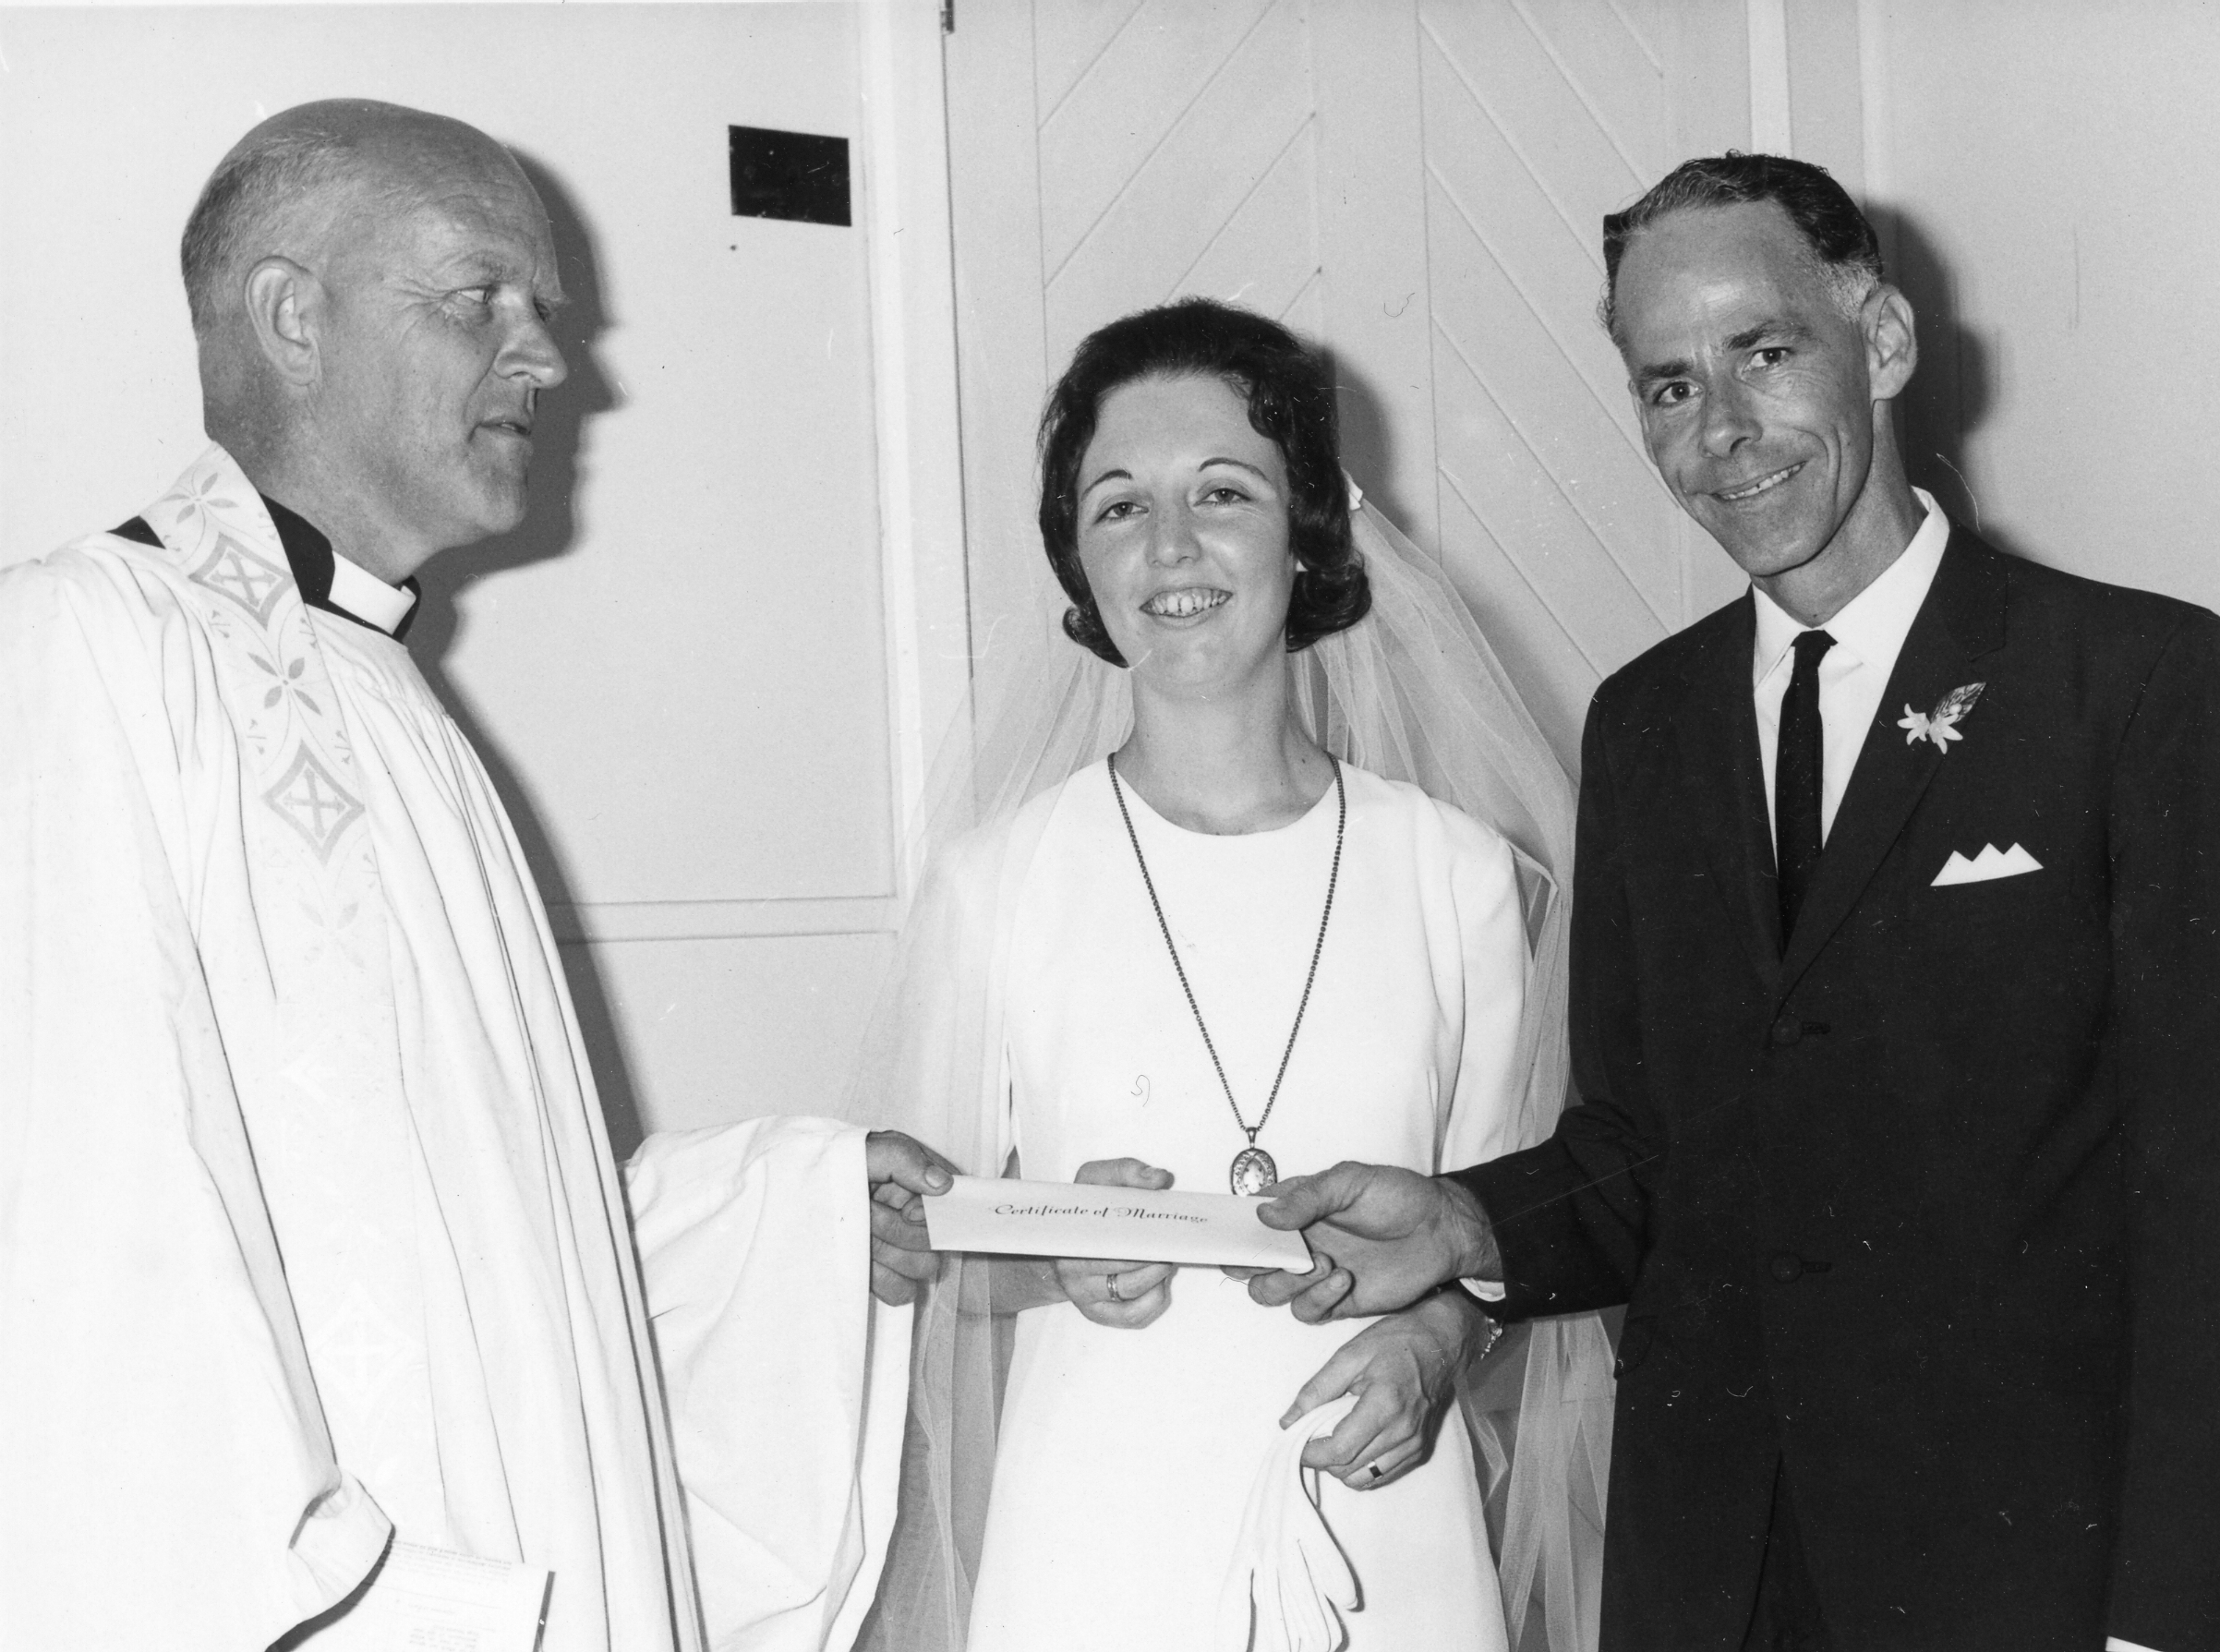
\includegraphics[width=1.\linewidth,center]{../images/donnaVestry.jpg}
\caption{Rev A Gerlach, Donna (Hanson) and Trevor Hindley}
\end{center}
\end{figure}


As related by son Michael, the family arrived in Murgon a couple of days before the scheduled arrival of the furniture removalist, and apparently walked in on a Ladies Guild Meeting in the church hall - much to the surprise and consternation of all, a story which Rev Alf delighted in relating in later years. Marion Kapernick was quick to offer hospitality, beginning a long and enduring friendships between the two families. Marion and husband Ivor (Mick) were reliable and consistent parish supporters until the Kapernicks' passing in 2018.

The mood was enthusiastic and positive; but behind the scenes, and of great concern to the parish administration personnel, was the looming figure of ever-increasing debt. As reported in a 26 September 1963 Diocesan Council minute, the parish secretary, C V Lord, under direction from the parish council, had requested Diocesan permission to move the Rectory Loan Account from the Commonwealth Savings Bank, Brisbane to the local National Australia Bank (NAB) `so as to receive a set-off from parish accounts.' Permission to proceed was granted along with the requirement to `arrange an overdraft limit sufficient to cover' the \pounds519.5.11 repayments arrears to Brisbane Account as well. This required a reduction of \pounds215 each half year at an interest rate of 5 \nicefrac{1}{2} \%.\footnote{Diocesan Property and Finance Board minutes 26 September 1963}

\section{First Parish Assistant Appointed}

As parish congregation numbers continued their rise, a need for `more complete pastoral care' and some relief for the rector's ever-growing work-load, was addressed in a parish council meeting where a brave decision was taken to employ an assistant.\footnote{Minutes of Parish of Kilkivan 6 November 1963}The problem of financing an assistant was somewhat mitigated by funding from the Diocese. Several letters are contained in Diocesan files referring to funding grants on the basis of perceived income gained from having a parish assistant. Miss Dorothy Ursula Evelyn Toon was appointed and was warmly welcomed to the parish and has taken up duties as Parish Sister.' She came to the parish from Coorparoo `after having completed two years training in Deaconess house, Sydney' where she received her diploma on 2 February 1964.\footnote{\emph{Church Chronicle} -- March 1964}

Youth Group activities were extended throughout the parish, reflecting Rev Gerlach's focus through his own call to faith. Additional Secondary School involvement in Murgon, Goomeri and Kilkivan increased by 50\% and no doubt contributed to growing Youth Group participation as did the more regular visiting in the outlying centres. Extra Sunday School classes needed to be introduced resulting in turn in outings such a picnics and even fancy-dress balls becoming features of the younger members' social calendars. The number of teachers and youth leaders grew in all centres to accommodate these growing attendances.

Sr Ursula's work put her in contact with Mothers Union in Cherbourg with the result that some of their members joined Murgon for a bus trip to Halse Lodge for a Rural MU Conference.\footnote{\emph{Church Chronicle} - 1964} Over 30 people attended a Youth Camp held on 23-26 April (cost \pounds3.10.0/each) conducted by Rev J Roper with all keen for a repeat.

Notice of plans for the rite of Confirmation to be administered on 16 September were issued with a call for intending candidates to register promptly for post-Easter classes and the Church of England Men's Society (CEMS) sponsored visit by `Jungle Doctor, Dr Paul White, who will preach at 10.00 am then address a men's luncheon gathering before flying to Toowoomba.'\footnote{\emph{Church Chronicle} - 1 March 1964}

The 7 February 1964 passing of Mrs Sing, a devoted member and `long-time President of the Murgon Guild who had been instrumental in guiding the Guild's lucrative fund-raising efforts towards the erection of the parish hall'.\footnote{\emph{Church Chronicle} - 1 March 1964}




\begin{figure}
\begin{center}
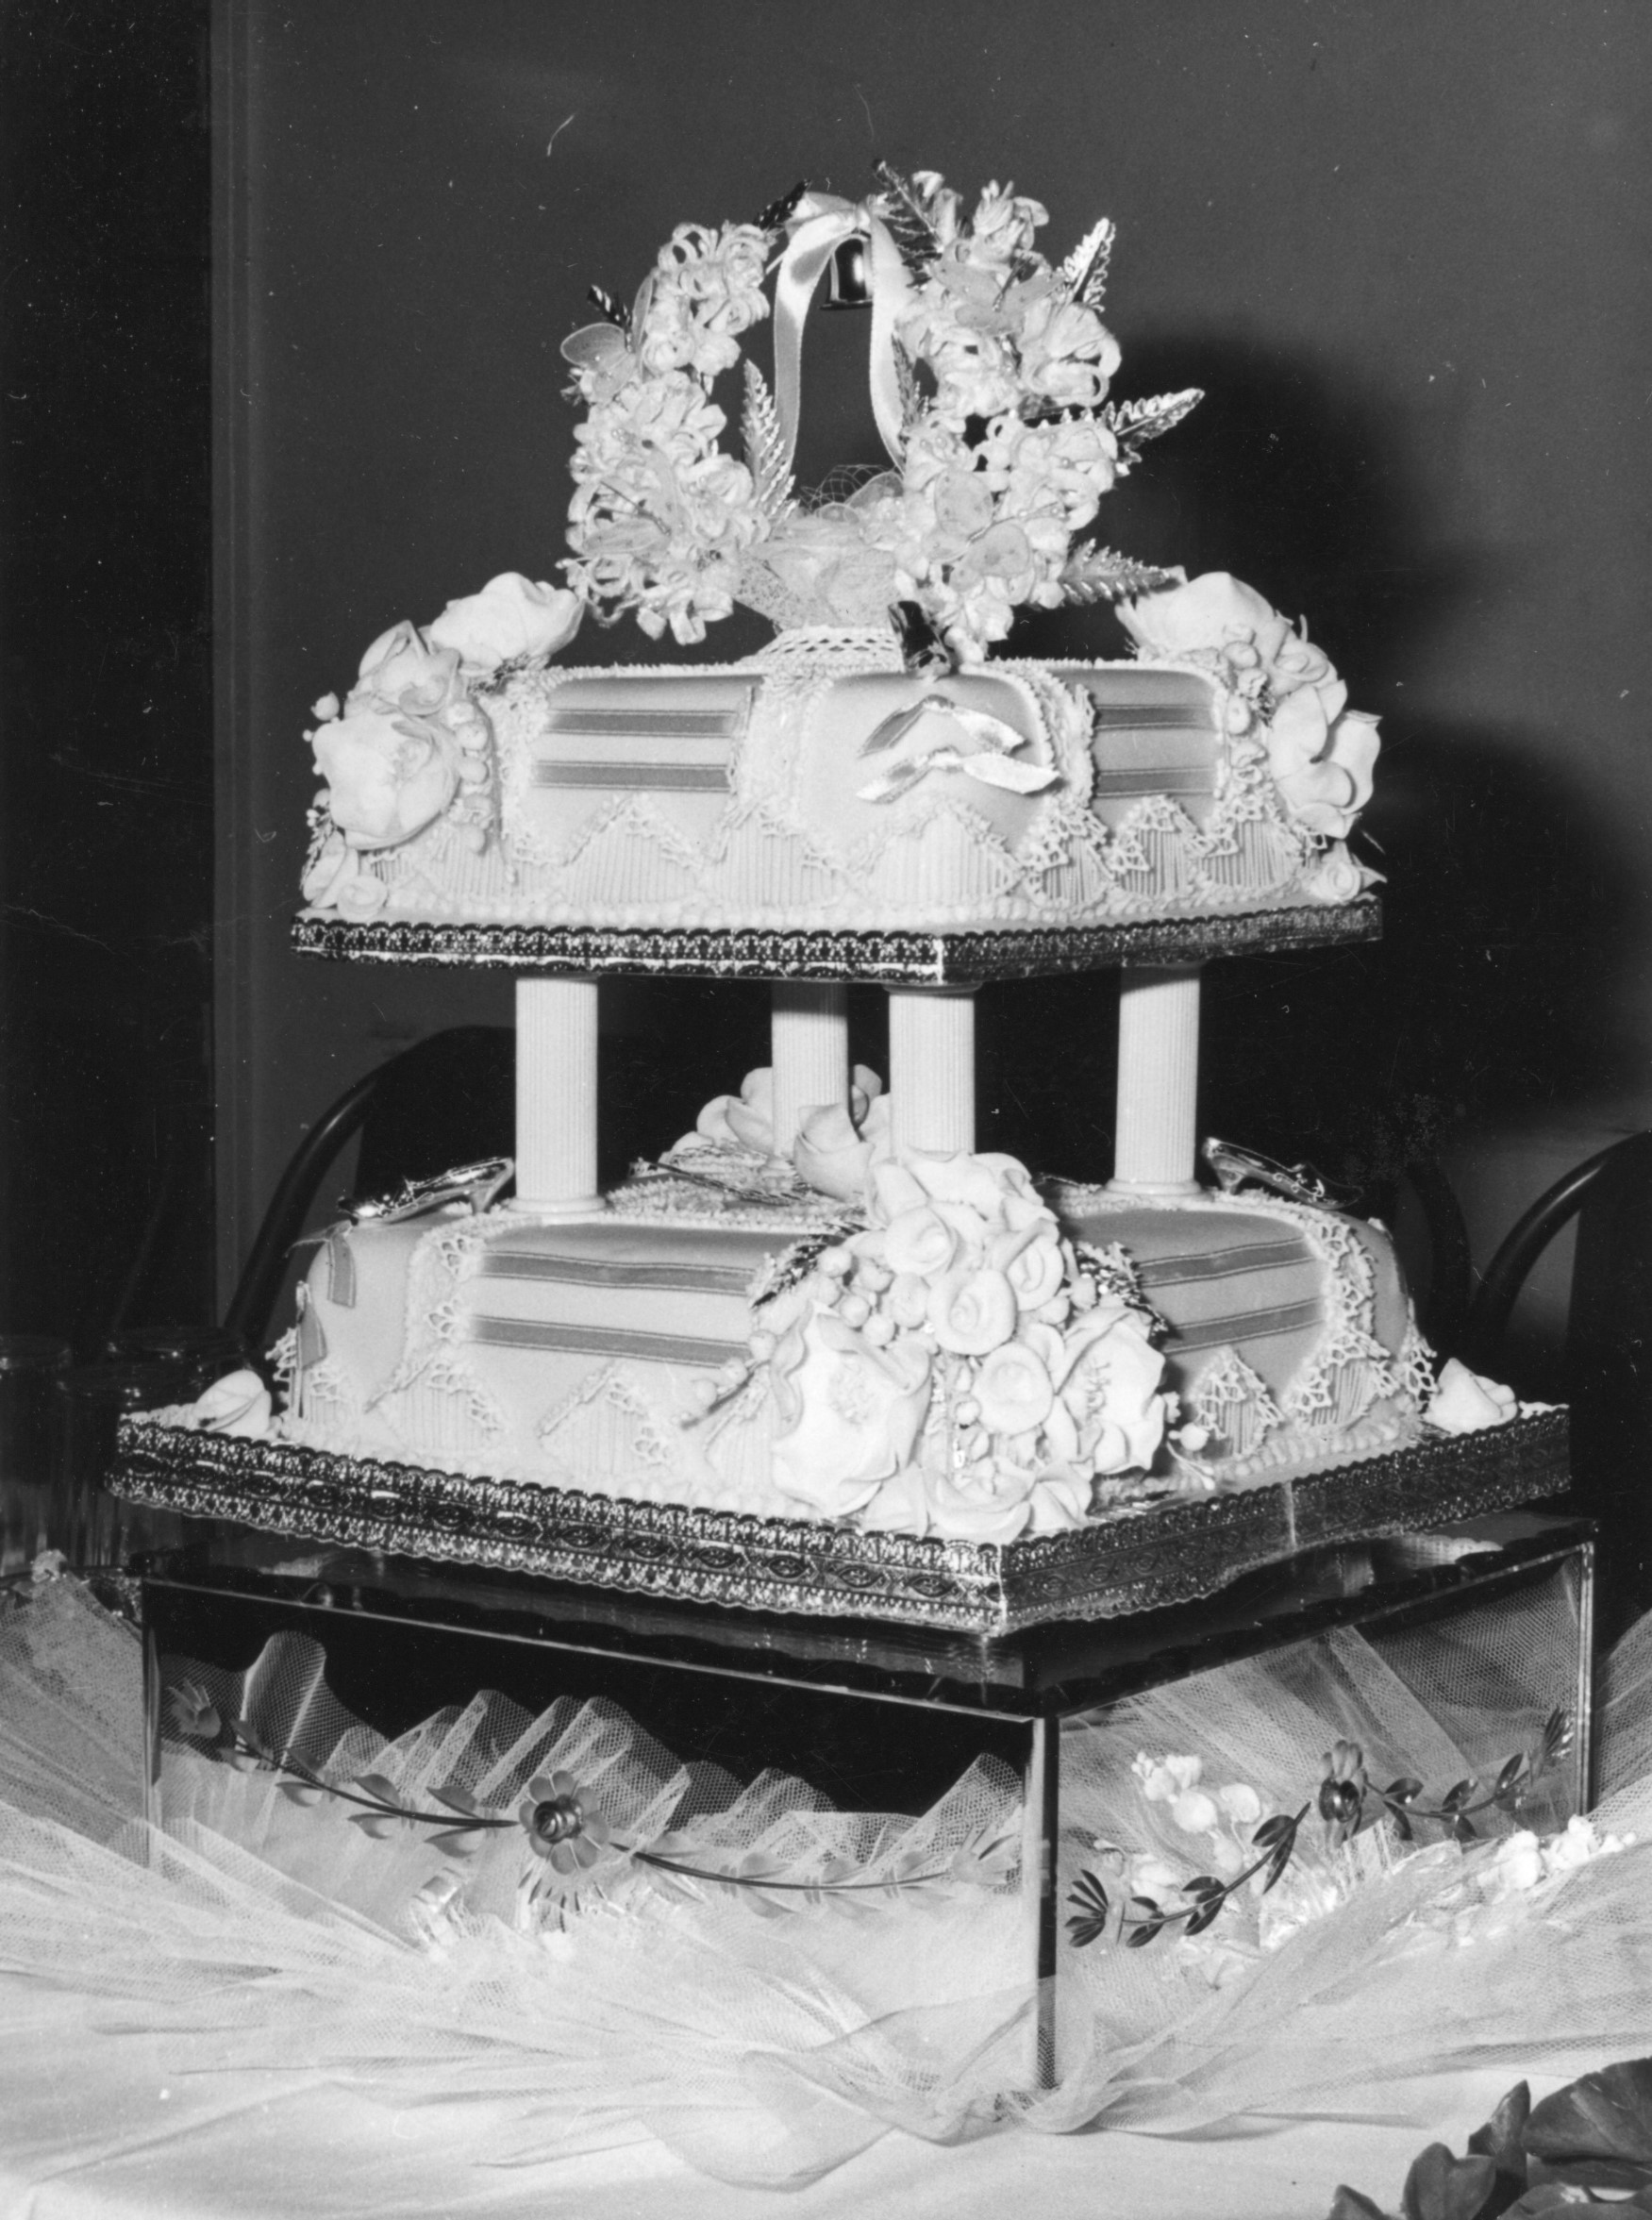
\includegraphics[width=.5\linewidth,center]{../images/donnaWeddingCake.jpg}
\caption{Wedding Cake, Donna Hindley}
\end{center}
\end{figure}


Archbishop Strong's first visit to the parish in September began with 33 well tutored candidates being administered the Rite of Confirmation in Christ Church Murgon. He later visited and inspected `Cherbourg Aboriginal Settlement, one of the largest of its kind in the Commonwealth and the only one in the Diocese of Brisbane.' His Grace conducted Evensong in the Church of the Holy Spirit and `met personally with congregation members after the service.'

The focus on extending Missions assistance continued with the 4 to 11 October 1964 Church Army Mission to Cherbourg by Captains Alan and Norman Polgen, where it was reported that many adults and children were brought into a deeper relationship with Christ. A special parishioners' gathering in Goomeri heard `much detail about the desirability to reinforce this ground-work through more effort being expend in the Cherbourg area' which had a population of 1200 with 700 being children. There were 11 teachers in the State School to cater for approximately 400 students over all seven year-level classes.

Lay involvement in services to include assisting in Rector presided sacraments and conducting Morning Prayer and Evensong services was encouraged. On 26 October, 1964, Albert Chisholm Mayne (Bank Officer, Murgon), Trevor Cichero (Pharmacist, Goomeri) were officially appointed as Lay Readers as was Mr Bernard (Bill) Ashmead Gedge on 1 November.\footnote{Correspondence File 1964}

Enthusiastic Lay personnel of the parish organized and conducted another Stewardship Campaign (with a Counselling element) which was well received and resulted in a substantial rise in parish income.\footnote{\emph{Church Chronicle} 1 November 1964 p 28}

\section{The Second Parish Assistant Appointed}




\begin{figure}
\begin{center}
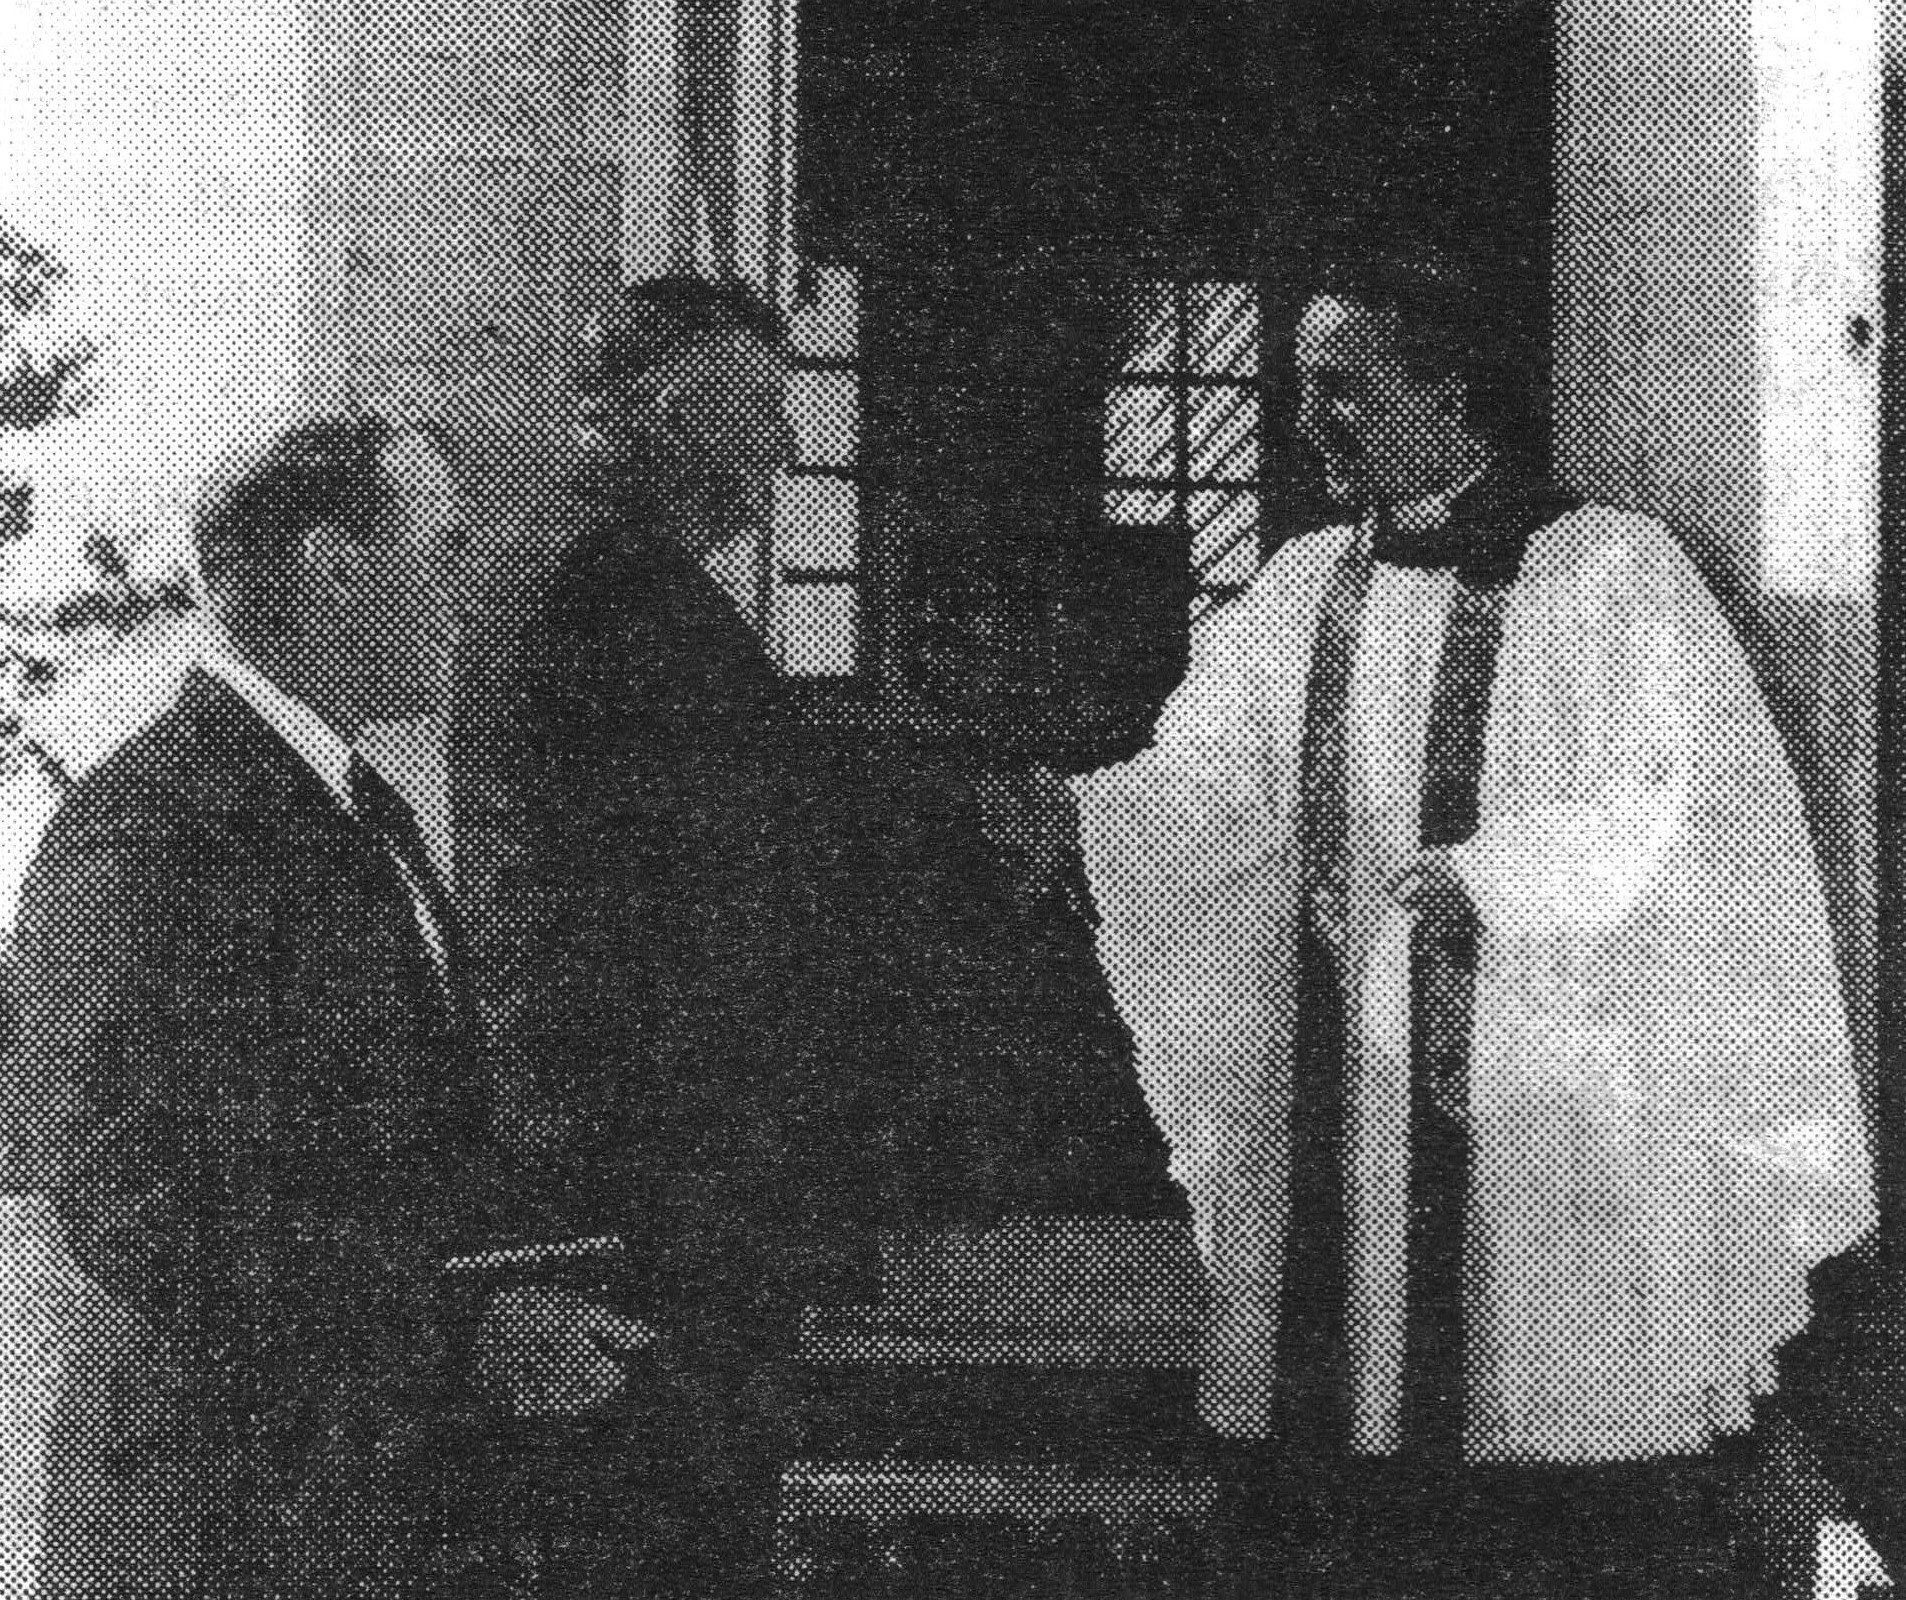
\includegraphics[width=1.\linewidth,center]{../images/DMcDougall.jpg}
\caption{Rev David McDougall}
\end{center}
\end{figure}


By 1965 the parish's Golden Years had truly arrived. A second Parish Assistant was considered a necessity to keep pace with growth in church attendance and youth involvement. In August 1965 a young and newly married 28-year-old `Catechist and Lay Reader', Mr David McDougall, was considered and approached to fill the void. He was admitted as Lay Reader in the Parish of Kilkivan on 19 July 1965 and made a Deacon in Bishopbourne on 28 August that year as noted in the Memoranda column of the parish services register.




\begin{figure*}[!htb]
\begin{center}
\includegraphics[width=1.\textwidth,center]{../images/davidMcDougall.png}
\caption{David McDougall Lay Reader's Testimonial}
\end{center}
\end{figure*}


By November 1965 the purchase of a Curate's House, 34 Taylor Street, Murgon, was in progress with G Roberts (solicitor) acting for both vendor and parish `at a considerably reduced cost'. Proposals were made to convert the property from Perpetual Lease to Freehold over a 20-year, interest-free term following finalization of purchase.\footnote{Correspondence File - August and November 1965}. Rev Gerlach reported in the February 1966 \emph{Church Chronicle} that the house had been purchased (at an economical cost of \pounds1500 secured by a mortgage), and renovations by volunteer labour, enthusiastically led by the competent Rector, allowed for insurance cover of \pounds2000 -- an immediate increase in value. David and Anne McDougall moved into their new home just before Christmas.

\section{A Rector and Two Assistants}

From July to December 1965, with two assistants working in-team with the rector, the parish took great steps forward. The November 1965 \emph{Church Chronicle} proudly carried all three names.

Canon G A Pearson led a `Mission to Murgon' (a teaching mission) that proved very profitable spiritually and in the practice aspects. Bishop Hudson visited and conducted the Rite of Confirmation.\footnote{\emph{Church Chronicle} November 1965}

In November 1965 Rev McDougal, with Diocesan grants support, undertook his `mission to the people of Cherbourg'. Rev Gerlach described this as `the most progressive step in the Diocese for many years.' and noted that `Already the response has been considerable'. \footnote{\emph{Church Chronicle} November 1965}

Other parish events included the Annual Spring Garden Fete and Mannequin Parade in Murgon (opened by the Venerable H J Richards), Goomeri's Successful Baby Show and Kilkivan's Annual Children's Fancy Dress Ball -- all hosted by local Guilds.

At this time, it was announced that Sr Ursula would `shortly be leaving to take up a similar position in Gympie'. \footnote{\emph{Church Chronicle} November 1965} Her departure was regretful and in part due to financial constraints in that Rev McDougall would now be supported `largely by the parish and parishioners, income will need to increase if a Parish Sister were to be retained as well.'.

Some Diocesan Grant monies continued in view of Rev McDougall's involvement in Cherbourg. With more regular services being conducted and attendances increasing with every `ringing of the bell', enthusiasm grew. A study group was organized with encouraging results. Volunteers began maintenance on, and painting of, the church building. Patrick (Paddy) Alberts became the self-appointed gardener and kept the grounds in immaculate order.

Of incidental interest was the August 1965 sale for \pounds5 of the original site of St David's Church, Boonara, almost 30 years after its removal to its present site, to Mr C Lord whose property fully encircled the tiny plot.\footnote{Diocesan correspondence}

\section{From Three to Two}

Sister Ursula Toon was farewelled on 5 December 1966 following Evensong in Christ Church, Murgon. Her `invaluable work in schools, GFS, Sunday Schools and Fellowships over the previous two years becoming almost a full-time Youth Worker' was greatly appreciated.\footnote{\emph{Church Chronicle} 1 February1966}

Rev McDougall carried forward the good work she had begun in the Schools and Fellowship areas while Lay helpers were enlisted for some other activities, thus allowing him time to continue to care for the residents of Cherbourg. He was a very popular young priest, and talented musician, who was active throughout the parish with an affinity for the outer reaches.

Capacity congregations in Murgon and Boonara were enthralled by Bush Church Aid Society's Rev John Wyn's description of working in vast, remote areas and the work of the Church's flying medical work in his Australian parish covering the 1000 miles of the Transcontinental Railway. A visit by Rev N Langford-Smith, Bishop of Nakuru, Kenya was planned for 5 March with 6 March 1966 Holy Communion followed by a Men's Breakfast in the Parish Hall. \footnote{\emph{Church Chronicle} 1 February1966}

The Easter Parish Meeting was set for 1 April in Goomeri to be followed by a `basket lunch'\footnote{\emph{Church Chronicle} 1 February1966}

Of historical significance, the services register of 22 May, 1966 records the funeral service of Rhys (Bill) Mander-Jones, the last member of the Jones family dynasty to serve the parish in active participation. He followed the tradition set by his predecessors David Mander and son Llewellyn Mander Jones of Boonara and George Hall and David Lacey Jones of Kilkivan -- all descendants to the level of great-grandsons, of the original David Jones, Sydney, the 1838 founder of the famous David Jones stores. An account of early Jones participation is contained in the Boonara Centenary Book (Diocesan Archives) and a large, framed, relevant section of the Jones family tree held in St David's church, Boonara. The late Mr R M Jones's Will left a sum a \pounds1,000 in trust with the Brisbane Diocese `\ldots to apply the income (the interest accrued) in maintaining St David's church of England, Boonara\ldots' When probate was finally granted, \$2,000 was applied (with accrued interest of \$373.33) as requested and monies have been accessed as directed to this day.

While 1966 was a remarkably vibrant year in parish life, the most exciting event for Rev McDougall would have to have been his Ordination to the Priesthood on 21 December -- a wonderful `Christmas Present' to him and to the Kilkivan Parish with two fully ordained priests there. The number of Sacramental services increased greatly with up to seven Sunday services being conducted and the use of the duplex envelopes resulted in a pleasing increase in Missions giving. On 6 August 1967, a typical Sunday, Rev McDougall covered Holy Communion at 7.30 am, Murgon; 9.00 am, Cherbourg and 11.00 am, Windera whilst Rev Gerlach went further afield for H.C at 7.30 am, Goomeri; 9.30 am, Kilkivan including a Baptism (Batts); 11.00 am, Boonara with a Baptism (McIntosh) and finally back to Murgon for 7.30 pm. The same page in the services register indicated two further baptisms, two funerals and one marriage (Lindsay Quinn/Cathy Burgess).




\begin{figure*}[!htb]
\begin{center}
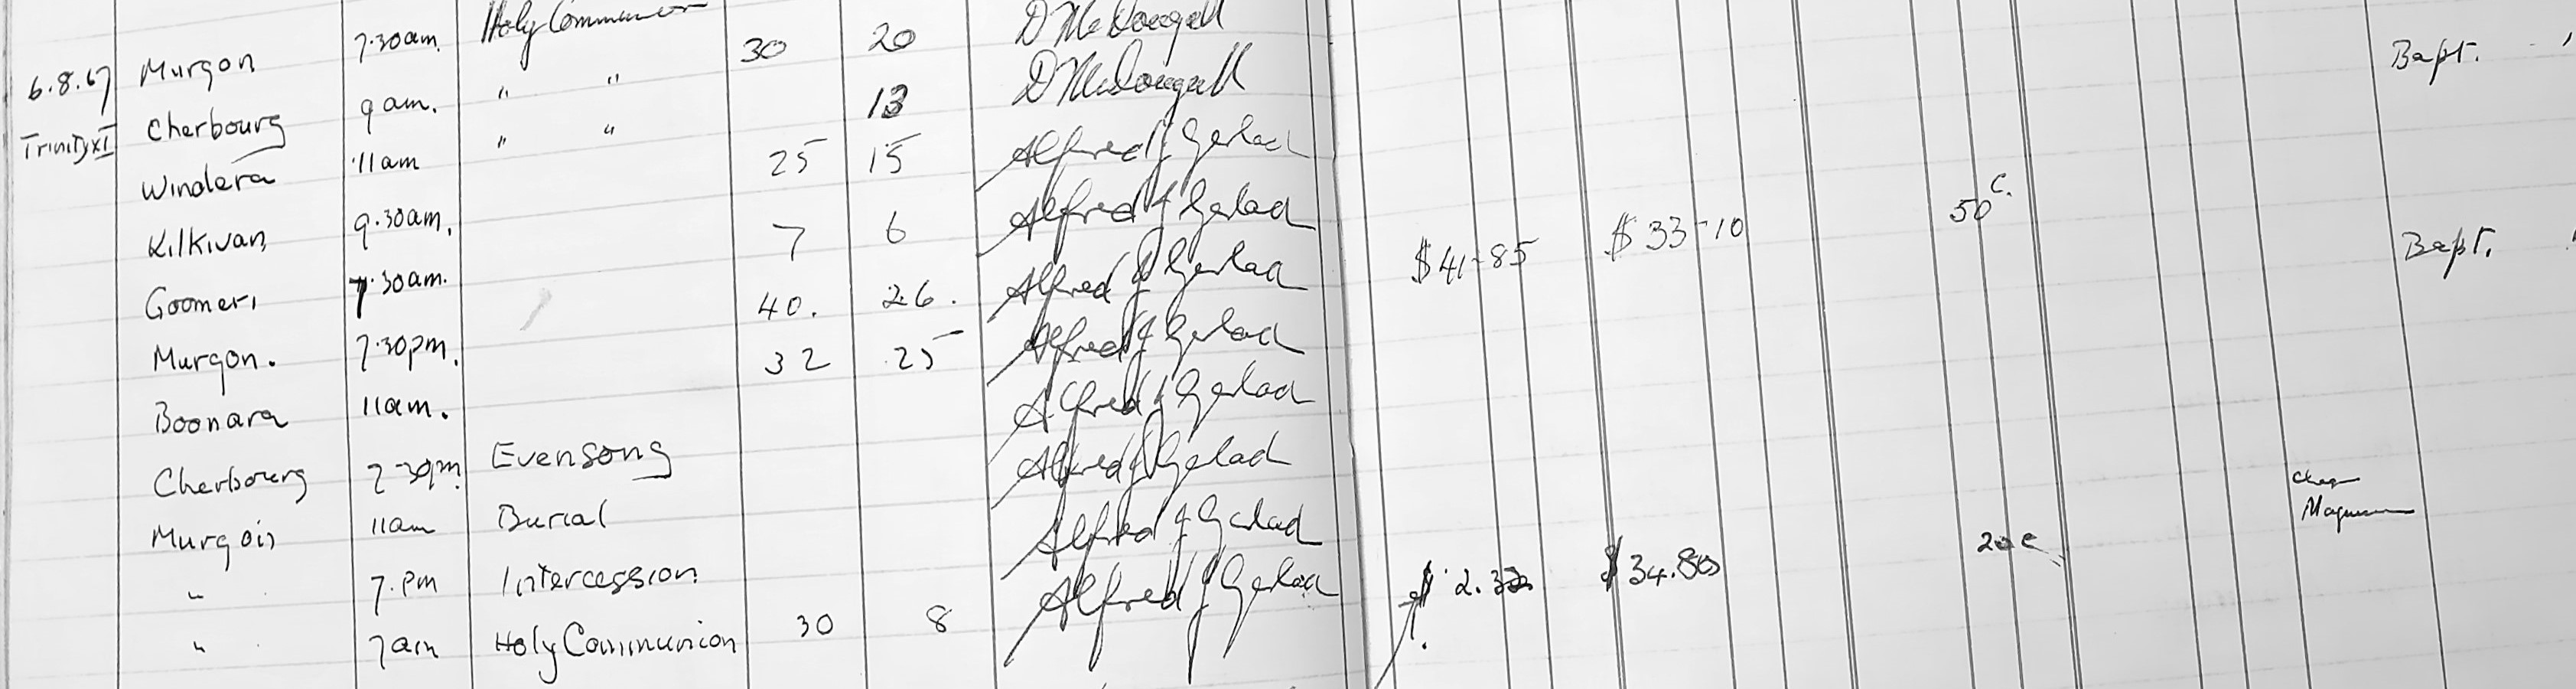
\includegraphics[width=1.\textwidth,center]{../images/serviceRegisterAug1967.jpg}
\caption{Service Register August 1967}
\end{center}
\end{figure*}


During this `time of two' parish activities proliferated. Five new members were admitted to the Mothers' Union group bringing the total active membership to over 40 ladies. Boonara church liquidated its overdraft, proceeded with repainting the building, and began a Bible Study group. Windera completed paying for its church which was dedicated in 1958. There were `plans' to extend the Parish's Hall due to heavy overcrowding in the Kindergarten section. Murgon Guild held a Garden Fete with the objective to raise funds for this venture. Parish coffers were frequently augmented from Guild funds raised through, for example, Street Stalls and Debutante Balls.

Although offerings income increased, with two salaried priests to support along with two houses and two cars to maintain, increases in cost-of-living items such as electricity, telephone and transport being added to the existing financial situation, it was evident that every blessing carried heavy responsibilities. By June 1967 budgeting issues resulted in a request to Diocesan authorities to allow a parish overdraft increase from \$4,730 to \$6,100 (as below) on the security of the existing guarantee

\begin{quote}
Present debt: \$4,730

Balance on Cost of New Car: \$577

Working account O/d repayments: \$668

Margin for working expenses: \$125

TOTAL: \textbf{\$6,100}
\end{quote}

As signed by Rev Gerlach and Parish Wardens C V Lord and L Sempf, repayments were to be \$630 half-yearly for 18 months then at \$430 half-yearly, in addition to interest charges.\footnote{Diocesan Correspondence Files}

However, even though some extra funding assistance was granted through the Diocese, this was largely taken up by salary increases and by 1968, `as usual in the history of the church' so often evident in this rural parish, reliant on the vagaries of weather for income, funds were once again at a critically low level and regretfully, Rev McDougall's services had to be let go. The unfortunate consequence of this was that some of the valued initiatives which had been implemented had to be pruned back while others were fully discontinued. These included some religious instruction classes in schools and, in one case, the Sunday School was discontinued.\footnote{Kilkivan Centenary Book p 18}

\section{Back to `One'}

With Rev Gerlach at the helm the run of Holy Communion services in the parish returned to the pre-assistants-pattern as indicated in this excerpt from a copy of the Parish News. Along with this busy schedule of Sunday services, week-day offices of Morning and Evening prayer were offered daily in Murgon.

Death is a part of life and so funerals also feature prominently in any Rector's diary. Two in 1970 which deserve mention are those of early 1900s settlers, Frederick W McIntosh of Tansey, buried on 1 June at Boonara after a 60-year connection with the church, and the untimely sudden death of long-serving parish member, Leonard Sempf (Kilkivan) which was greeted with shock and great sadness by the entire parish. He had served as centre warden at Cinnabar in the early years then later as peoples' warden for Kilkivan centre and as rector's warden for the parish, many years a parish councillor, plus duty as synod representative. The later granting of a Faculty by His Grace the Archbishop, Felix Arnott, allowed Mr Sempf's memory to be honoured by the installation in St Matthew's, Kilkivan, of a Silky Oak Pulpit made from timber cut from his Cinnabar property -- a gift from his wife, Lil.

With many family units attending services, there were many baptism and weddings as well -- sometimes almost too many on one day as of 20 December 1969.

The service register shows three weddings in one day: 11am, Reginald Smith/Janelle Maudsley -- Kilkivan; Noon, Richard Row/Margaret Roach -- Kilkivan; 4pm, Riley/Weasel - Murgon




\begin{figure}
\begin{center}
\includegraphics[width=1.\linewidth,center]{../images/weddings19691220.png}
\caption{Weddings 20 December 1969}
\end{center}
\end{figure}


In 1968 David McKie (an Accountant in Murgon) agreed to take the helm as Secretary Treasurer of the parish and moved to address some of more legal requirements of the Diocese such as a `Local Constitution' for each centre and issues concerning consecutive non-attendance at Parish Council meetings `without leave of absence' and thus being `deemed to have vacated his office'. In August 1968. a bank account, separate from the general Working Account named Christ Church Murgon Building Fund was opened, spurred by a bequest of \$500 from loyal parishioners, Mr and Mrs Tate through Mr Frank Narracott, for `the express purpose of' extending or building a new church in Murgon. A request for recognition in some way on new work was an added requirement. A Diocesan held Tate Bequest still stands.

During the latter part of 1968 Mr Norman Steel Thornton, employed by the Public Service Department as Deputy Manager at Cherbourg was appointed as a Lay Reader.

The 50\textsuperscript{th} anniversary of Christ Church's April dedication in 1920 was celebrated over two weekends. On 12 April 1970 the church hosted a Murgon Jubilee Marriage Reunion service followed one week later with Golden Jubilee Eucharists at 7.30 am and 9.00 am with Archbishop Philip N W Strong officiating and preaching. Refreshments in the hall followed. A special Golden Jubilee Appeal for Missions was held over the month of April. Associated with this, ``Kath Braithwaite and Sylvia Adams arranged a programme for the Parade of Brides wearing wedding gowns of each decade, interspersed with songs form each decade.'\footnote{A Short History of Christ Church Murgon M U -- MU 25\textsuperscript{th} Anniversary Service Booklet, 14November 1985}

During November 1970 Ross Desmond Waters and Ivor Douglas Kapernick of Murgon were licenced to `conduct Divine Services in the Parish of Kilkivan. In 1972, Trevor Cichero, who over the past nine years had held positions of Lay Reader, Sub-warden, Sunday School Superintendent and Parish Treasurer at some stage, sold his Pharmacy business and left parish to further his calling to the Priesthood.

Rev Gerlach's interest in youth work underpinned an energetic Lay focus in that area. Murgon resident, Ross Waldock, reminisces:

\emph{I became a member of Church of England Boys Society (CEBS). Great times. We camped at Kinbombi Falls with Mr Doug Kay and Mr Stuart James. Mr James told great stories of his time in the Northern Territory. I wore the backside out of my shorts sliding down to the water hole at the bottom of the falls.}

\emph{My sister Karen became a member of Girls Friendly Society (GFS) along with Roslyn Dennien and Lyndall McAntee. The CEBS and GFS had social dances in the new hall.}

\emph{We also combined with Goomeri, Murgon, Windera and Cloyna for a trip to Halse Lodge at Noosa Heads in Noel Petersen's new bus.}

\emph{Rev Alf Gerlach took us out to the Forrestry at Gallangowan and Jimna -- up the Fire Towers!!! -- then on to the Bunya Mountains to the new TV stations. Fantastic trip in Rev Gerlach's Peugeot 403 (:\ldots the only car to have\ldots').}

\emph{I (Ross) became a Server for Rev Gerlach. Other Servers were my cousin Graham Mickan, Alan and Geoff Moreton, Darryl Trapp, Neil Mayne, Neil Trapp and I think the Milton Boys.}

\emph{Confirmation was a big event and filled the church.}

During their time in Bellingen (1958-`63), Mrs Shirley Gerlach, a nurse by profession, became seriously ill with Hepatitis to a critically near-death point. Her recovery was considered by all as a miracle of prayers answered by God. Rev Gerlach stated openly that during this time he was plagued by a short period of doubts, but through Shirley's `miracle` his restored faith was firmly cemented and deepened to levels he had been unaware was ever possible along with an unshakable belief in the healing power of God through prayer. He supported and encouraged involvement in the church's `Order of St Luke'. A small group was introduced in Murgon following visits by Mr and Mrs Alex Learmont (Vancouver) in connection with the Ministry of Healing sponsored by the local chapter of Order of St Luke with a Healing service held periodically on a week night.

Hardships encountered in his early `between the wars' life meant Rev Gerlach was well equipped to counsel with empathy, those in need or trouble. He was also a warm and encouraging supporter of anyone who needed guidance in their faith journey. It stands as a testament to this empathetic fostering of potential that two of his flock, Trevor Cichero and Ross Waters, both heavily engaged in parish affairs, were moved to seek his approval for training for Holy Orders. Dr Ruth S Kerr (née Fraser), historian, long-time public servant in research and native title and now Adjunct Professor in History, School of History and Philosophical Inquiry, The University of Queensland, St Lucia, wrote of her personal appreciation for this support while a young teacher and Christian in Murgon in 1969.

\emph{``Rev Gerlach delivered stimulating and thought-provoking sermons based on the bible readings for the day. He and wife, Shirley, played a very influential role in my faith development.''} \footnote{Dr Kerr's personal correspondence.}

The financial position in the parish caused the Gerlachs concern to the point where Mrs Shirley Gerlach, while always giving her husband unconditional support in his varied roles, added a financial facet by returning to her nursing career at the Goomeri hospital. When this facility closed its doors around 1968, she moved on to the hospital in Cherbourg. While this deviation from the traditional `Minister's Wife' role, so clearly illustrated in former years by such as Mrs Ernie Smith and Mrs Donne, initially raised a few quizzical eyebrows, her nursing prowess soon overcame that. Her reputation as Matron at the Cherbourg hospital and later on in the Sunshine Coast region until retirement to Toowoomba remains legend.

As life has it, all good things come to an end. Archbishop Arnott's hand written diary

entry for 6 February 1973 records `The resignation of the Reverend Alfred John Gerlach Th L as Rector of the Parish of Kilkivan has been accepted to take effect as from 17 February 1973'.




\begin{figure*}[!htb]
\begin{center}
\includegraphics[width=1.\textwidth,center]{../images/gerlachResignation1973.png}
\caption{Archbishop Arnott's diary note}
\end{center}
\end{figure*}


He and Shirley moved to Palmwoods (1973-1981) and Maroochydore (1981-1990) and was appointed Rural Dean -- Sunshine Coast (1987-1990). After `retiring' in 1990 he worked as an Honorary Assistant in Maleny parish until relocating to Toowoomba in 2002-2012, continuing with Permission to Officiate in St Luke's.

\section{Gone but not Forgotten}

`Gone but not Forgotten' could have voiced by both the Gerlach family and the Parish of Kilkivan. Alf and Shirley returned for several milestone events in Parish life, the last major one being the 2014 St David's, Boonara, Centenary where Rev Gerlach proudly accepted Archbishop Aspinall's invitation to present the Gospel reading and to assist in administering the Eucharistic Sacrament. He later spoke warmly of his memories of being Rector in the parish.

In what some may consider a sad, but rather beautiful twist of fate, two funerals took place -- one In Murgon and one in Toowoomba -- of two couples whose kinship in Christ spanned almost 60 years.

On 17 December 2018, a large gathering (including members of the Gerlach family) in Christ Church, Murgon celebrated the lives of their Christian brother and sister, Ivor (Mick) and Marion Kapernick, who were then buried together in a single grave after having passed into eternal life just four days apart.

Eleven months later, on 14 November 2019, at St Anne's Church, Highfields, Alfred and Shirley Gerlach were also celebrated and farewelled from this life, having also journeyed in to eternal realms a week apart and now are at rest, side by side. Many church dignitaries, including the Bishop of the Western Region, Right Reverend Cameron Venables, were present along with a large gathering of friends and family (including Kapernicks). The most moving aspect of this gathering was the very large contingent of friends from or with past connections to Cherbourg, to honour a Minister they loved and trusted and knew had their welfare firmly in his focus, and his wife, their `Matron Gerlach' whose revered memory will be forever in their hearts.

If ever we need a true example of God's purpose for marriage -- the uniting of two persons, husband and wife, into `one flesh', we have it in duplicate here. United in life, united in death, united in the Hope of the life to come. Truly Beautiful.
\balance

\printendnotes[custom]
\setcounter{endnote}{0}
\chapter{1973--1979 : Rev Donald Keith Campbell}
\nobalance

I am deeply indebted to the Archdeacon Emeritus, and very good friend, Donald Campbell, for his personal contributions which, when directly quoted, appear in \emph{italics.} (Marcia McIntosh)

Once again, the parish was without a resident priest. From 17 February 1973 onwards, the parish register of 3 March 1973 indicates the faithful Bill Gedge's regular pattern of a 7.00 am Morning Prayer service in Cherbourg, then on to 9.30 am Goomeri, 11.00 am Kilkivan and ending with 7.30 pm Evensong in Murgon. He was given some reprieve when Archdeacon L W Grayson presented three services on Holy Communion (Murgon, Goomeri and Kilkivan) on 25 March. The same pattern was repeated on 22 April (Easter Day), also with Holy Communion, thanks to Rev J G Harrison.\footnote{Parish of Kilkivan Service Register February to April 1973}




\begin{figure}
\begin{center}
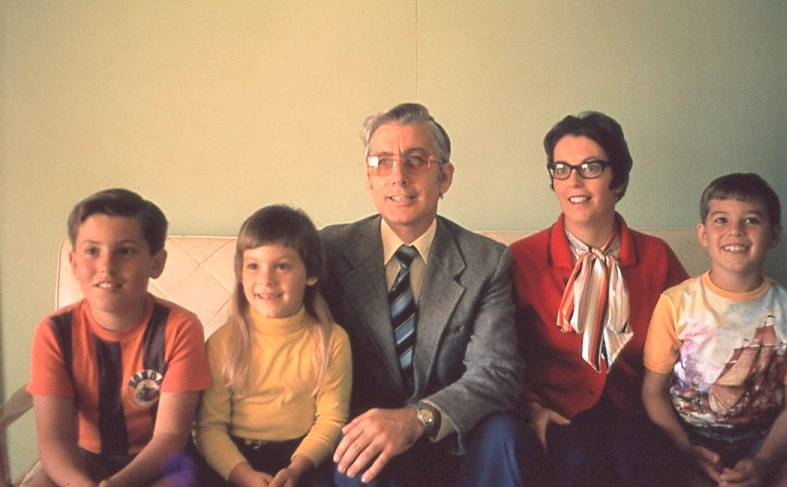
\includegraphics[width=1.\linewidth,center]{../images/DonCambellAndFamily.png}
\caption{Rev Don Campbell and family}
\end{center}
\end{figure}


The funeral service for Mrs Kate Stephens (incorrect spelling of `Stevens' in register), one of the pioneers of the Kitoba area between Cloyna and Windera, conducted by the Rev W G Hayston on 3 April is noted. \footnote{Parish of Kilkivan Service Register February to April 1973}

During this time letters and phone calls were being exchanged between the Diocese and parish's wardens and nominators, conferring over a list of ministers considered as possible candidates to fill the vacancy. On 7 March the parish representatives were advised that, for various reasons, Rev G O Thomas had decided he could not accept their offer of the position of Rector. A further nomination was requested. After several unsuccessful nominations by the Kilkivan Parish, on 12 March 1973, Parochial Nominators I Kapernick, C Lord and K Batts wrote: `After careful consideration, we would be very happy to have the name of Rev Donald Campbell put before the Presentation Board as a new Rector for our parish.'

Archbishop Arnott's letter of 2 April 1973, carried the glad tidings of Rev Campbell's acceptance desire `to take up residence in June following the birth of their third child expected in May\ldots' He continued, offering to investigate the possibility of Rev Jack Harrison being available `to take services over Easter' and his willingness `to act as Locum Tenens until the Campbell family arrived'. Archbishop Arnott was also very keen to visit and officiate at Rev Campbell's induction service -- `possibly after Synod'.\footnote{Diocesan Correspondence Files}

The Diocesan Year Book lists him as `Donald Keith Campbell, B.Sc (Uni of Qld) 64, ThL (ACT) 68: Dip. R.E (MCD), Th Schol (ACT) 1972. He was ordained a Deacon in 1968 and Priest in 1969, served as Assistant Curate at St Stephen's, Coorparoo (1968-1970) and then at All Saints, Booval (1970-1973).\footnote{Diocesan Clergy Records P 24} Engaging this young, enthusiastic priest, with wife Lurline and three small children (Simon, Paul and baby Ruth, just a week old) was considered to be a positive step for the parish to take, in order to move forward with youth work and community involvement in church activities. Many changes and new initiatives began to be introduced -- not the least of these being the singing of choruses accompanied by the Reverend on his guitar.

The new rector had a connection with the parish as his father, Mr Alex Campbell, had been the Head Teacher at Kilkivan school in the late 1950s. This stood him in good stead with the Kilkivan congregation who gladly accepted him as a `local'. He soon learned that travelling through the parish often involved uninvited encounters with local wild-life. `Roo Bars' and spotlights were noted as frequent features on the locals' vehicles -- saving enormous damage bills but not at all advantageous to the poor `Roos.

\section{First Service and Induction}

Rev Donald Keith Campbell conducted his first service in the capacity of Rector of a parish on 3 June 1973 at 7.00 am in Cherbourg, followed by 9.00 am, Goomeri; 11.00 am Kilkivan, concluding with 7.30 pm in Murgon -- a busy day, meeting many parishioners , none of whom ever word name badges. His Induction followed on 28 June in Murgon. \footnote{Rev Campbell's correspondence}

Supported by a solid team (Wardens D Kay and I D Kapernick; Lay Readers, B Gedge and I Kapernick; Synod representatives, E A Williamson and L Sakrzewski), work began immediately and progressed through 1973 on a steady basis.

\emph{`On arrival in Murgon I discovered that as well as taking services at six centres I had also inherited 19 Religious Education classes at the primary schools at Murgon, Cherbourg, Goomeri and Kilkivan as well as at the High School at Murgon. Over the next few years with the Ministers' Fraternal we moved to an ecumenical approach and had the Ministers and Lay volunteers take normal classes spread over the week and not just denominational groups. I succeeded so well that just before we left Murgon, I was only taking one class which was a class that no one else would take on as they were `too tough'.'}

Innovative as ever, Rev Don, as he became known to the students, decided to break the lesson into different short spots as well as using visual aids for the main lesson. One was a `Ha Ha' spot (jokes at which they groaned but wanted them to continue); others were `Did you know?', `Dear Donald Dix' and `The Serial'. Books were read in serial form, always managing to stop at a crucial point, leaving the students waiting for `next week's instalment'.

The regular Services roster (as indicated in the section on Rev Gerlach) which had stood for many years was followed. However, they were not all at consistent times each week, plus Murgon, the chief centre, was only being offered a Holy Communion service twice monthly.

\emph{`\ldots when Bill Gedge came to Christ Church Murgon for a 7.30 am service on the Sunday it was scheduled for 7.30 pm, it seemed we had to re-think the whole matter of times of services. Associated with this was the fact that Boonara and Windera had one 11.00 am Sunday service a month and a 2.00 pm Sunday service. The afternoon services were nearly impossible in high summer.'}\footnote{Rev Campbell's correspondence}

Rev Campbell is quoted as saying: `\ldots as summer progressed the sleepier we all became \ldots{} it was bad enough when the congregation went to sleep but when the preacher also `dropped off', things had to change.'\footnote{Boonara Centenary Booklet, p.30} A new, more regular schedule offering more Holy Communion options was trialled. \footnote{Rev Campbell's correspondence}

A rather faded Fordigraph (Gestetna)-printed issue of the parish's magazine, \emph{Telling All People}, set out the new service proposals allowing Holy Communion to be offered in five centres every Sunday except for the occasional 5\textsuperscript{th} Sunday services where only three services were scheduled.

Every Sunday Murgon was offered a 7.15am Eucharist using the traditional Prayer Book form of service. A new \emph{Australia 1973} Prayer Book (The Green Book), had been successfully trialled in the parish. The 9.15am service adopted this modern form and was more family oriented.

A 5.30 pm option for Cherbourg was also introduced but changed later to 6.00 pm on all Sundays; Goomeri: 1\textsuperscript{ST} Sunday @ 7.30 pm and 4h Sunday @ 11.00 am; Kilkivan: 1\textsuperscript{ST} and 4\textsuperscript{th} Sundays @ 11.00 am; Boonara: 2\textsuperscript{nd} Sunday @ 11.00 am and 4\textsuperscript{th} Monday (later changed to Tuesday) @ 7.30 pm.\footnote{St David's Boonara Services Register 1923 -- 1993}; and Windera: 2\textsuperscript{nd} Monday and 4\textsuperscript{th} Sunday, both @ 7.30 pm, with a more informal Communion Service. \footnote{St David's Boonara Services Register 1923 -- 1993}

\emph{`The intense discussions we had in the vestry afterwards at both Boonara and Windera over supper were a highlight. The topics ranged from politics to prices of wheat, pigs and beef to ethical issues and deep theological questions. They were great times.'}

Such was the interest throughout the parish that there was only one problem with filling Parish Council positions -- the many nominations and the necessity for a voting process! The AGMs were traditionally held in Goomeri's Church of the Epiphany, following a service of HC. However about two years into his incumbency, the overwhelming congregational interest was so great that tradition was broken and the AGM was transferred to Goomeri's Show Pavilion to take a more relaxed, picnic form of luncheon. While the serious, adult meeting-business was in progress, a number of `brave' volunteers oversaw games and activities for the children in the spacious grounds.

On 21 February 1974 Lloyd Sakrzewski was admitted to the Office of Reader in the Parish of Kilkivan and Bernard Ashmead Gedge's licence approved for renewal. Later in the year John William Stanton also became a licenced Lay Reader, thus allowing for more Morning or Evening Prayer services to be added to the schedule. The rector produced notes for the lay readers. While the Duplex Envelope option for offerings, first introduced by Rev Donne in 1958, was available and encouraged not all parishioners adopted its usage. Notes in the register list both offerings as `Envelopes' and either `Open Plate' or ``Loose Change'. The `missions' side of the envelope received some attention resulting in an increase in the parish's missions' contributions.




\begin{figure}
\begin{center}
\includegraphics[width=1.\linewidth,center]{../images/duplexOfferingEnvelope.jpg}
\caption{Duplex Offering Envelope}
\end{center}
\end{figure}


Guild activities proliferated, funds from street stalls and catering for functions were often boosted through the efforts of Bill and May Gedge in their vegetable garden in Gore Street and the sale or use of its bounty\emph{.}

\emph{`When we arrived in 1973 Bill was a widower. From the Church of England Vegetable account Bill Gedge was able to provide the funds to buy the new technical device -- a Fordigraph duplicator -- so now the weekly notice sheet could be in colour. His efforts also funded an overhead projector. While it was cumbersome it allowed the use of visual aids in the services. Several times a year Rev Don brought bookstalls from the CMS Bookshop to all the centres.'}

On 16 May 1975 permission was granted for the use of the \emph{Australia 1973 Prayer Book} for a further 12 months. An application to install a Conn Electronic Organ in Murgon, signed by Rector and wardens Kay and Kapernick, and forwarded to the Diocese on 30 May 1975 was approved and a Faculty granted by Archbishop Arnott, dated 10 July 1975.\footnote{Diocesan Correspondence Files May 1975} Under the magic fingers of (mostly) Gwen Kay and Marjorie Surawski, the notes from this lovely instrument boosted the beauty of Murgon services.

Goals and Aims for 1976 and beyond were all aimed at continuing the growing momentum seen throughout 1975 and 1976 .

The ambitious list for the three-to-six-months periods included; starting Confirmation classes by 31 May. The introduction of a September, after-school `G-Kids' series in Goomeri and one in November in Kilkivan.

Neighbourhood Interest in Bible Studies (N.I.B.S) groups in each of the six centres was fore-shadowed.

Plans were in hand for a Family Camp and setting up displays (bookstall, posters, puppets, singing groups etc) at the Murgon, Goomeri, Tansey and Kilkivan Shows and Camp-draft events in 1977\emph{.}

\emph{`There was also an outreach activity in the main street of Murgon one Saturday morning, on the back of a truck. At one stage we had a large group of children really enjoying the singing and action songs. A group of adults then appeared and ushered them away. It seems that there was a regional gathering of Jehovah's Witnesses in the Murgon hall that weekend and our effort was not appreciated by the adults.'}

In the Winter, 1976 TAP parish magazine, the three-year goal was headed `\textbf{CANCELLED!'.}

While it had been the goal to have a parish assistant (curate or parish sister) in three years, `after debate this idea was rejected by the meeting as a 3-year goal, and was instead adopted as \emph{a 6}-\emph{month goal'}.

Though the magazine's name was later changed to \emph{Shalom,} the wide and varied topics were of great value and fostered a whole-of-parish connection and brought insights into the church activities beyond local horizons.\footnote{Parish Magazine \emph{Telling All People} (TAP) Winter, 1976, Volume 2, Number 1}

Rev Campbell organized and led an empowering preparation course at a Bunya Mountains Confirmation Camp for 19 young parishioners on the theme, `a Time For\ldots' The Fight Reverend R E Wicks presided at the Confirmation service on 3 October 1976.\footnote{Parish Magazine \emph{Shalom}, October 1976}

Parish Council's considered opinion was that `there is more than enough work for two people to do in the parish' over and above the supporting input of the many lay volunteers in all areas. The consensus was emphatically directed to continued growth in the Youth section, maintaining vigorous Sunday Schools in almost all centres with particular mention of the very well attended one in Cherbourg, as well as maintaining and further promoting the Healing Mission of the Order of St Luke. All were urged to foster more involvement in existing ventures and by encouraging contacts to assist with hospital and home visiting of people in the local area, lead or participate in home Bible Study groups, encourage greater church attendance and so on - all simple and easy things for a willing heart, but of immense assistance to the ever-growing list of Christian ministry duties open to all.

An early spring edition of the parish magazine (TAP), reinforced Rev Campbell's focus on the missionary aspect of all church involvement, highlighting the ABM's Mission in the Carpentaria area of coverage - northern Cape York, the Torres Strait islands and into Papua; CMS's work in Tanzania; the parish's aim to send a group to the CMS Summer School to be held in Burleigh Heads, 13-19 January 1976. The publication also dealt with matters of budget; a review recommended reading of the Book of the Season - `The Escape', by Viola S Winn (\$2.20); a history of Joseph Mohr's hymn `Silent Night'; various other thought-provoking items such as `Can I be a Christian and not go to Church?' and much more.\footnote{Parish Magazine \emph{Telling All People} (TAP) Spring, 1976, Volume 1, Number 2} This appears to have been the last TAP issued before the name changed to \emph{Shalom}.




\begin{figure}
\begin{center}
\includegraphics[width=1.\linewidth,center]{../images/workingBee.jpg}
\caption{Getting the new tank up on the garage roof}
\end{center}
\end{figure}


Travel in a parish with six centres, three of them country towns, two rural ones plus the Cherbourg Aboriginal Settlement, some more than 50 km apart, was obviously a big issue. Ministry to the six centres and, in the early days to take the R.E. classes in the schools, meant Don was frequently on the road. One day he was returning from the school at Kilkivan and as he \emph{`came over the brow of a hill there were two large trucks side by side coming up the hill and very close. Some parts of the road were very narrow through cuttings but fortunately there was some room off the road at this spot and all three vehicles passed with inches to spare'.}

After three years as their rector, Don Campbell had begun discussing with the Parochial Council how the parish might be more effective in proclaiming the Gospel and building people up in their faith. Various outreach options to nominal Anglicans and others desirous of deeper investigation of spiritual issues had been considered.

\emph{`At each of the six centres we began to have an Annual Festival followed by a meal. Regular attendees were encouraged to invite their nominal friends and relatives. These services were well received and some who came were encouraged to come more often.'}

\section{The Bethel Bible Course}

This led to the idea of training people to be leaders for home groups. To do this, confident leaders were needed. For confidence in faith and a solid understanding of the Bible, the Bethel Bible Course idea was floated, receiving positive response in spite of the lengthy period of dedicated study required. Even some of the more elderly were moved to hone their learning skills and techniques. Much credit must be given to the rector for the encouraging and persuasive manner in which he promoted and implemented this course.

The Bethel course involved 26 sessions of 2 \nicefrac{1}{2} hours. The Old Testament was covered in the first year and the New testament in the second year. It was very demanding, and 21 people signed up for it in 1978. One group met on Tuesday evenings in Murgon with a smaller group on Thursday evenings in Goomeri. Each session had an illustration to help people remember the main points of the lesson. Sometimes large amounts of the Bible were required to be read before the actual study. The group members did this and lives began to be changed as people grew in their understanding of God's Amazing Grace in sending the Lord Jesus to reconcile us to Him and to each other. The catchcry for the Bethel course is ``Blessed to be a Blessing'', based on Genesis Chapter 12, verses 1-3.

With such clearly evident and firm congregational support behind `their man', the search

for a suitable Parish Assistant began in earnest. Miss Joan Evelyn Gray, a trainee at Deaconess House, Sydney was approached and was happy to be nominated. Due process was followed and a letter signed by Archbishop Arnott was received consenting to her appointment as Parish Assistant, (initially on a one-year basis as an experiment), beginning with a salary of \$6,300 per annum with a house, car, gas and electricity etc. paid by the parish. Rev Campbell's 12 October 1977 correspondence with the Diocese announced her starting date as 1 February 1978. One of the stated aims of her employment was `to assist with the Bethel Series in the Parish'.




\begin{figure}
\begin{center}
\includegraphics[width=1.\linewidth,center]{../images/sundaySchool.jpg}
\caption{Sunday School. (clockwise from left) ?, Christopher Henness, Phillip Jackson, Cieran Edmonds, Josh Baker. Stephen Henness, Daryl Skeehan}
\end{center}
\end{figure}


It would also seem that, during this same late 1977 period, Rev Campbell's successful handling of `all things parish' had been noted as his hand-written letter to the Archbishop expressed regret that he `did not feel he could accept the' invitation to move to Booval parish at that time', mainly because the parish had funded two weeks in Sydney in September `to learn about the Bethel Bible Course'; he was the only one trained to lead it in the parish; more people than he had `ever dared hope' had enrolled; he felt leaving at that point would `negate much of the aim' of endeavours so far'. The response from Brisbane was `very understanding of his position\ldots' offered blessings for continued work there and to the Campbell family for Christmas.\footnote{Diocesan Correspondence Files 1977}

\section{Archie the Glove Puppet}

Among the initiatives was the introduction in Murgon of a Family Service once a month. To gain the children's interest and attention, a glove puppet named Archie would suddenly appear from behind a board. Later a transportable puppet theatre was built for the parish and this became a favourite part of the Family service. Archie developed a reputation as a `\emph{Smart-Alec know-it-all}'. The theatre's reputation grew and its activities were extended to other centres in the parish and beyond. By 1977 a thriving Youth Group with nearing 20 members operated in Murgon. Some of the boys helped operate other glove puppets and met mid-week to record the dialogue\emph{.}

\emph{Joan Gray also became a `straight-guy' to Archie. It is even more amazing that these segments were greatly appreciated in spite of the fact that they were largely ad-lib. As a further outreach the parish ran a stall at the Murgon show one year and showed film strips relating to some of Jesus' parables (the high tec of the time!). Puppet Archie also featured and sometimes his habit of being rather confronting and saying things that a human person couldn't, caused a bit of a stir. There were occasions when children became so upset, they ran up and punched him in the face!}

It could be said the goal of gaining attention and involvement was fully achieved.

\section{Beach Mission at Elliot Heads}

In 1978 the Campbells were invited to lead a Scripture Union Beach mission at Elliott Heads near Bundaberg during the January school vacation period in the latter half of the 1970s. Some 10 parishioners joined the first SU team drawn from a number of denominations. A training day was held for the whole team during the November/December period. Each Evening glove puppets told the story of `The Lion, the Witch and the Wardrobe' by C S Lewis.

\emph{The script needed 6 Puppeteers at various time and in the final battle scene it needed some ingenuity to have 13 puppets on show at the one time. It was a real hit not only with the children but with many parents. Some came each night and left when the puppets finished. On the last evening questions to the children showed they had really understood the message.}

The parish supported these Elliot Heads Missions for three consecutive years but were discontinued after Rev Campbell left the parish. Some of Joan Baker's photos

\section{Youth Safari}

In May 1979 it was decided to take a coach load of teenagers on a Safari up through Monto and Biloela to Rockhampton. The group stayed in church halls. It was a very valuable time with study/talk, discussion each morning and activities in the evening as well as travel and sightseeing. The boat trip to Great Keppel Island was a highlight.

As priests are often required to change parishes, housing is provided. The Rectory at Murgon is most comfortable and very suitable but after his incident and close-call with the semi-trailers, Don realised that if anything happened to him, Lurline had no place to go with three small children. After self-funded study at Theological college, the Campbells had few reserves but `\emph{with God's help through loans from kind relatives and a sympathetic bank manager',} they managed to get a deposit for a small cottage at Caboolture. To help with repayments, Lurline started to do supply teaching at primary and high state schools in the area as well as a stint at the Convent. She continued to lead a Bible Study at Cherbourg and to be involved in Parish and Christian Women's Convention International activities.

Murgon had three Service clubs, Apex, Lions and Rotary. Don was invited to join Rotary which led to valuable contacts in the Community for him and Lurline. He was President one year. Another outreach into the Community came through a series of `Belt the Rector' evenings when parishioners would invite their friends to their homes when they could ask and discuss any questions they wished.

The 1979 services roster in the parish for the main centres appears to have remained almost unchanged from the 1975-1976 roster with Rev Campbell's signature appearing against all Holy Communion services in the parish each Sunday. In addition, Joan Gray's signature was attached to several Morning Prayers services in Murgon as well as the other parish centres, showing a great increase in the opportunities for worship within the parish.\footnote{Parish Services Register etc}

\emph{On my return from the Youth Safari in 1979, there was a letter from the Queensland (with Northern NSW) branch of the Church Missionary Society inviting me to be the next General Secretary of the Branch. I felt honoured to be considered but my immediate reaction was to decline as I felt committed to finish the second year of the Bethel Bible Study course at the end of 1979. I phoned one of the members of the CMS Committee and said that I would have to decline as I was committed to stay in the parish at least till the end of the year. ``Yes, we know that, and we will wait!'' That caused me to stop and think and pray. If the offer from CMS was of the Lord maybe there was another way to approach the situation. To this end, in consultation with the Wardens and Parish Council it was decided to send Mrs Marcia Mcintosh to the Bethel training course. Marcia took over the course and at the end of September the Campbells moved to Brisbane after more than six wonderful years in the parish.}

The 1 June 1979 Diocesan Council noted that an official letter of resignation had been received from Rev D K Campbell to take effect as from 1 October 1979 and its official acceptance by the Archbishop, The Most Reverend Felix Arnott. This was communicated in writing on 10 July 1979 to Mr D H Kay (church warden). \footnote{Diocesan Correspondence Files}

At Rev Don's last Parish Council meeting as their rector, Warden Ewen McIntosh expressed the parish's sincere and deep appreciation of the benefits, advice, spiritual guidance and fun times all had received from him and from his wife and family through their drive and enthusiastic involvement in all activities.\footnote{Parish of Kilkivan Minutes 3 September. 1979, p. 116}

It was with great regret but with sincere congratulations on his posting that a large number of parishioners farewelled the family on Sunday 30 September. Rev Campbell conducted two H C services in Christ Church, Murgon that day, the first at 9.00 am, then a 10.30 am Family Service\footnote{Parish Register} followed by luncheon in the hall. Lurline Campbell's 1979 diary notes prompted Don to reflect:

\emph{`Apparently the packers came on Tuesday 25th. We must have gone to our new home in Gloucester Street South Brisbane, unpacked and come back for the farewell. I was commissioned as General Secretary to CMS in St John's Cathedral on Friday 14 September, by Archbishop Arnott'}

All services thereafter until November were conducted by Joan Gray.\footnote{Parish of Kilkivan Service Register}

Following his commissioning, Rev Campbell commenced his work as Missions Chaplain, and General Secretary CMS in September 1979, a position he held until 1993 when he became Rector of Surfers Paradise. During this time he also served as a member of the Aboriginal and Islander Affairs Committee and became Archdeacon of the Gold Coast from 1995 until 2004 when he retired. Archdeacon Emeritus Donald Keith Campbell and his wife Lurline, now reside in Upper Coomera, where they are active in St Matthew's, Coomera, one of three centres in the Parish of Gold Coast North. The font from St Matthew's Kilkivan is now in this centre.\footnote{Clergy Notes}
\balance

\printendnotes[custom]
\setcounter{endnote}{0}
\chapter{1979--1990 : Rector -- Rev Victor James McNamara}
\nobalance

During the four months following the announcement of Rev Campbell's impending October departure, Parochial Nominators Doug Kay, Keith Batts and Geoff Baker sought a suitable nominee to fill the vacancy. A Diocesan-issued list of available priests was carefully studied, settling on Rev Victor James McNamara. Once approached, and with Rev McNamara's favourable response in hand, approaches were made for his official nomination `as our choice of Rector' on 3 August, 1979 while Rev Campbell was finalizing his departure.




\begin{figure}
\begin{center}
\includegraphics[width=1.\linewidth,center]{../images/mcnamara.jpg}
\caption{Rev Victor McNamara}
\end{center}
\end{figure}


For the purposes of organizing the Archbishop's very crowded diary, as early as 5 October 1979, the Archbishop's office contacted Mick Kapernick (for discussions with other Wardens and their nominee) re the possibility of Archbishop Arnott's flying to Kingaroy or Wondai for a possible service of Induction for Rev McNamara in November around 3.30 pm on a Saturday, followed by a later service in Cherbourg. Alternatively, the Induction could occur at 7.30 or 8.00 pm on the Sunday.\footnote{Diocesan Correspondence files}

The concept of taking light-plane flights for such occasions was a marked change from the days of half a century earlier when travel to these areas was, at best, by train and sometimes lasted up to a week. Even when the new rectory was constructed in the 1950-1960 period, one bedroom was specially designated as the `Bishop's Room'. The motor car did enter the scene fairly early on, but the idea of a literally `flying-visit' was only just becoming a reality.

Another graduate from Moore Theological College, Sydney, Rev McNamara was ordained Deacon in 1972. He served as Assistant Curate in Dalby (1972-1975), and was ordained as Priest in 1973. He accepted the position of Vicar of Jandowae in 1975 and served there till his move as Rector to the Parish of Kilkivan in 1979.\footnote{Diocesan Clergy Records p. 29}

Kilkivan parish welcomed Rev McNamara, wife Doreen and their five vibrantly energetic children (Angela, Andrew, Wendy, and twins Timothy and Kirsty) to the parish in mid-November, 1979. The rectory again rang to the sound of happy young voices. His electrical and wireless/television technical skills were soon put to good use by the locals who were also happy to welcome a priest with a love of and great interest in cricket. Rev Vic carried on the tradition of `ministers with their endearing eccentricities'. At least at Boonara, he was soon noted for leaving the door of his car open during service time, the radio on, `\emph{to check the scores}!' when an `important' cricket match was being played. An added bonus for him was the continuing presence of Miss Joan Gray as Parish Assistant along with a co-operative and cohesive Christian community.

Rev McNamara's first official duty as Rector was to conduct the 17 November Holy Matrimony service for Kennedy/Beasley. He began his services rounds on 18 November with Murgon's 7.30 am and 9.15 Holy Communion services, then on to Goomeri at 11.00 am, Cherbourg 6.00 pm and a hurried trip to Kilkivan for 7.30 pm Holy Communion there.\footnote{Parish of Kilkivan Services Register November 1979 DJ 3, Box 5}

The following Sunday, 25 November 1979, after conducting a 7.15am Eucharist with 40 present and 33 communicants, the day was spent preparing for his 3.00 pm official Induction. An overflowing local congregation was present to witness Archbishop Felix Arnott perform this rite. An impressive list of dignitaries - Archdeacon L W Grayson; Rural Dean and Rector of Gympie, B Q Scragg; and Rectors: Philip C Robinson, Nanango; Bill Ross, Wondai; Michael Scragg, Maryborough; R G Walsh, Rector, and Rev S James, Kingaroy; and C E Brook, Noosa, signed as witness to Archbishop Arnott's signature.

Rev McNamara was officially welcomed by Mick Kapernick, warden, on 4 December 1979.\footnote{Parish of Kilkivan Minutes, 1979, p. 118} The Year Book for the period indicates a dedicated parish with an active support team working with the Rector. Doug Kay and Mick (I D) Kapernick continued their long service as Wardens with Doug Kay, Keith Batts and Geoff Baker holding the position of Parochial Nominators. There were 22 Sunday School teachers over four centres with a total of 184 students enrolled; 22 Baptisms; 13 young people were confirmed and 13 Marriages solemnised. Following a subsequent Annual Meeting Keith Batts was joined by John Waldock as Synodsmen.\footnote{Diocesan Year Books both p. 82}

Planning was underway for the proposed Youth Safari 80. Under the leadership of Max Patten, painting of the Holy Spirit church at Cherbourg was underway with local volunteers. All 21 persons had successfully completed the two-year Bethel course. Marcia McIntosh was leading the parish into the Congregational Phase with groups being formed in all interested centres. The men's five-day September fishing trip to Fraser Island had come and gone with a nice lot of fish to show for it. The only `cloud' was that once again the parish's overdraft situation of \$2,936.32 on the rector's arrival, had now risen steeply to \$5,517. However, this was not viewed as a great problem since all expenditure was expected to produce financial gains. Direct giving, a new concept for consideration, was floated. Conservatism prevailed with promises `to give it some thought' along with the strong recommendation for the envelope system to continue. There was even optimistic talk of hiring another person with a specially dedicated role of Parish Youth Person. The only variation to the services roster was the introduction of whole-of-parish services on the 5\textsuperscript{th} Sunday services -- a great fellowship opportunity for all centres to come together for worship. The first of these coincided with the 30 September farewell to the Campbell family.

On 2 August 1980, the Murgon Mothers' Union ladies `provided the dinner after the Thanksgiving and Rededication Service, taken by Bishop R Wicks, on the occasion of our church's Diamond Jubilee.\footnote{A short history of Christ Church Murgon's MU -- M U 25\textsuperscript{th} Anniversary thanksgiving Service booklet 14 November 1985}

With the parish moving along energetically, annual three-day visits by Bishop Bruch Schultz became an eagerly anticipated Confirmation service event. A particularly early highlight occurred when Archbishop Sir John Grindrod, who had taken up the position in 1980, was welcomed to the parish where he conducted the Rite of Confirmation with Holy Communion on 17 September, 1982.

Throughout 1979 and into the early 1980s the signatures of both McNamara and Joan Gray appeared in regular pattern as officiating at Holy Communion and either Morning or Evening Prayer respectively, throughout the parish. Occasional services were delivered by other ministers and lay persons, such as S James, Bill Gedge, Mick Kapernick and Ewen McIntosh. The parish was well served in this regard. During March 1983 the Diocesan Registrar, N C Reid advised that Bruce David Boucher (Murgon), Henry Derek Collins (Cherbourg) and Marcia Gay McIntosh (Boonara) were officially accepted to be licenced as Liturgical Assistants -- Mrs McIntosh with a full licence, allowing her to conduct services, preach, and conduct funerals as well as the other LA duties such as administering the chalice. Mick Kapernick's licence was renewed. Later, Shirley Waldock was admitted as a Liturgical Assistant, so along with Keith Batts in Kilkivan, the parish was well covered with local lay assistance -- their names appearing frequently in the registers as officiant. The McNamara family took their annual vacation leave, post-Christmas/early January, and almost all services in this period were conducted by lay persons.

Rev McNamara was well-versed in church law and protocols. He is credited with bringing the parish into `the age of the computer', using his word-processing skills in continuing to produce the \emph{Shalom} magazine and for office communications and sermon notes. He added many interesting articles and comments, using the pen-name \emph{`Don Vittorio'}. Some parishioners were of the opinion that he was `spending too much time in the office -- at that computer!' With administration duties continuing to grow, a part-time office secretary, Mrs May Maudsley, was employed.

The sacramental services of Baptism and Marriage remained as a feature of priestly routine, as did the inevitable funerals, though some of them were conducted by licenced lay assistants.

Funerals on two consecutive days in August 1982 were noted -- that of Irene Sharpe in Murgon on 15\textsuperscript{th} followed by a 16 August funeral for the McNamaras' old friend, Malcolm Keith Grundy, which involved a return trip to their former parish of Jandowae.\footnote{Parish services register, 1 Sept 85}

From the late 1970s, the vagaries of weather again impacted heavily on this largely farming community. A prolonged drought was mitigated slightly by occasional advantageous rainfalls, though the often-optimistic hopes of a bumper crop were mostly dashed by rapidly returning dry conditions or storm-rains and which also reduced or totally destroyed final yields. Repercussions were felt in the dependant organisations throughout the area.

By 1981 parish finances were feeling the increased pressures. Normal cost--of-living salary increases for the two staff members were accepted without question. Diocesan stipend rates for Rectors had, by August 1981, increased to \$10,420 pa. At the monthly parish council meeting, Sharon Lord (secretary) was directed to contact the Diocesan Registrar, Mr Norman Reid. advising that along with supporting a priest the desired aim was to `\emph{work towards keeping an assistant in the Parish\ldots finances have been difficult this year and we find we cannot meet an assessment of \$3,900.'} A reduction to \$3,000 was mentioned as a possible commitment for 1981 and forward.\footnote{Diocesan Correspondence files 11 August 1981 and 26 August 1981}

Regretfully, by late 1981, due to pressing financial issues, the parish was forced to relinquish Joan Gray's valued services. Assistance given by the Lay Assistants became even more valuable and appreciated, especially in the smaller dependencies such as Windera and Boonara -- a great benefit with no reduction in opportunities to worship at their local churches. Grant monies for ministry to Cherbourg, through the Diocese from the Mary Peattie Trust Fund continued, and their value grew in significance.

By 1983, Rev McNamara began trialling mid-week Friendship Services in Goomeri and Kilkivan, mainly as a pastoral outreach to the elderly and mothers with young families who found it difficult to attend church at the scheduled Sunday times. These were relaxed, productive devotional times where even the most energetic and vocal children felt welcome. These proved to be a valuable addition to the schedule for the duration of his incumbency, resulting in increased participation in activities, Guild membership as just one example.

Visits and talks by Gideons International became more frequent and their efforts supported. Former pharmacist and valued and highly involved church member, Trevor Cichero, returned to conduct the 20 May 1983 funeral of local resident and friend, Tony Shaw. Goomeri has a habit of `drawing people back'.

The succeeding years were studded with memorable events in parish life. Growing community interest and involvement in service is evident through the signatures of lay persons including N Greenbury, M J Somerfield, J S Rea, E Wessling, N Smith, D Boucher in Murgon alone, accepting simple chores of accounting for the offerings. Other centres followed this same trend with great local involvement with Glen Maudsley's name appearing regularly in Boonara and Rob Solomon's and T McAntee's in Windera.

In 1983 the parish was again blessed with the presence of His Grace, the Archbishop Sir John Grindrod for a 9.30 am Confirmation service.

Also, in November, Murgon hosted the Mothers' Union 25\textsuperscript{th} Anniversary Service, led by V McNamara with guest presenter, Rev R G Walsh (Kingaroy). With 100 attending and 80 receiving Holy Communion it was acclaimed `a very successful day'.

Amusing comment: The 17 November, early morning H C Service in Kilkivan, (9 in attendance and 7 communicants). \emph{No men present!} \footnote{Parish services register entries 11, 15, 17 November, 1983}

Bishop Bruce Schultz visited the parish several times over 1983 and 1984, twice for three-day visits and for input into a Confirmation Camp. One Rector's report in 1983 speaks of a successful Town Mission and a suggested follow-up Country and Western Gospel event. The congregational phase of the Bethel Course continued and apart from a call-out for more volunteers to take Religious Education classes in schools, participation in all activities was at a high level. Parish Council applied to the Murgon Shire Council for the erection of road sign directing people to churches in each of the parish's towns.

As the years rolled by, this parish, with Murgon as its hub, continued to be noted for its support of projects great and small in all of its centres, no less so during McNamara's incumbency, several carrying parish historical significance.

In June 1983, the rector and parish wardens applied for a faculty to install a memorial lead-light window depicting the parable of The Sower in Goomeri's Church of the Epiphany, in honour of the pioneer Beresford family, to be made in Gympie by R and J Harrison. Duly granted under Archbishop Sir John Grindrod's signature.\footnote{Diocesan Correspondence files, 1983 - 1984}

\emph{Shalom} mentions the dedication in 1984 of a silver plated, gold lined Chalice. Suitably inscribed, it was donated by the Quinn family in memory of Joyce Quinn (McIntosh), grand-daughter of pioneer and churchman, Richard Maudsley whose daughter Ethel McIntosh had died following her daughter's birth in 1919. Joyce's husband, G C (Chappie) Quinn also a churchman for many years in the parish.\footnote{Shalom, Vol 9, No. 5, p. 9, 1985 and Boonara Centenary Book p. 18} The thread of enduring connection remained evident through many baptisms and weddings was again visible through the 1 October 1986 funeral of a second of Richard's daughters, Elizabeth Pretoria McIntosh.\footnote{Services Register 1986} A new Altar cloth was presented in her honour.

However, life and death go hand in hand. The funerals on one particular page the 18 entries in the Parish Burial Register for 1984 are devoted almost entirely to historically connected Murgon names -- a great loss to the Anglican church and the town. With reference to church life, two in particular stand out.

Parish `icon', Bill Gedge (80) left this life in July 1984 passing quietly while seated behind the wheel of his car, neatly parked in his garage, having just returned from a trip down-town. At his request, he was cremated at Albany Creek Crematorium. The parish honoured him with a Memorial Service in Christ Church Murgon on 30 July 1984. Rev Alf Gerlach returned for this sad but special occasion. Active till his last breath, Bernard Ashmead (Bill) Gedge's legacy lives on through the imposing presence of the Parish Hall and in the memories of all who knew him.

86-year-old Kathleen (Katie) O'Neill's death is registered two lines below. She also is considered a church and community `icon' having held many positions in Murgon church's Guild and was actively involved in `all things Murgon'. Two sons followed her example -- David in Kilkivan and Richard in the Murgon area. \footnote{Parish of Kilkivan Burial Register, current from 1919} Insert photo of page from Register

Rev McNamara seemed to have a particular passion for Baptisms and knack of presenting them `with a difference'. In September 1985 he undertook six baptisms in one 7.00 pm service at Holy Trinity church Windera, admitting Melody Jane and Cara Curtis, Tenielle Maree Kratzmann and Belinda, Michael and Tony Green into church family membership.\footnote{Parish of Kilkivan Baptism Register and Holy Trinity Windera, Services Register.} Around this time F G (Graham) Drew began conducting Morning Prayer services at Windera, in particular.

From \emph{Shalom}, of June 1986 referring to the baptism of Leah Hatton, Rev McNamara followed his usual custom of mixing both hot and cold water `\emph{so the temperature of the water does not unduly disturb the baby. However, to his consternation, he had put too much hot water in\ldots{} the fetcher of the required cold water'} was heard to comment: `\emph{He is the first minister that I have ever met who gives swimming lessons to a baby when he baptises it!'} \footnote{Shalom, Vol 10, No. 3, June 1986}

The Boonara services register of 9 October 1988 records the baptism of Mrs Alice Stumm. Quoting the Shalom article, she `took the plunge' as far as Christian commitment is concerned \ldots when she was baptised beside Boonara Creek. Thirty people including husband Paul and two children, Daniel and Michelle, were present to see Alice take this very important step in her life\ldots' While the event was `beside the creek' Alice was not immersed, though creek water was used in the ceremony.\footnote{Shalom, Vol 12, No. 5, October 198819} She took the next step of Confirmation on 29 October 1988, in the ceremony conducted by Bishop Arthur Malcolm. Bishop Adrian Charles officiated similarly on 2 December 1990 confirming 14 local young people.\footnote{Parish of Barambah Confirmation Register. Church Office, Murgon.}

Former parish member and very good friend of the McNamara family, Rod O'Mara, recalls a 1988 parish-hosted visit from Bishops George Browning (Brisbane Diocese, northern region). Bishop Browning shared Rod's interest in Bush Walking and, at the Bishop's request, an expedition to Barambah Falls in the steep gorges on the Boonimbah Road through a Galloway Downs property was undertaken. Several church members accompanied them. Rod provided the accompanying photo with the notation indicating himself, Bishop George Browning, Tim, Wendy and Andrew McNamara and Eddie Wessling were pictured. Rev Vic was also present but behind the camera. The visit is recalled in the Boonara Centenary booklet where `the parish was blessed with a double Episcopal visit over the weekend of 11-13 March. Bishop George Browning was accompanied by Bishop Arthur Malcolm. Boonara church was graced with their presence for the 11.00 am Eucharist which was followed by luncheon at Phillip and Sharon Lords' home.'\footnote{Boonara Centenary Booklet, p. 28}

Rev McNamara is noted for his generous effort to promote parish unity. Whole-of Parish events became a regular feature of the church calendar, beginning with fifth Sunday services which rotated through the centres. There were parish picnics, bus trips for business and for pleasure, while combined Guild events such as Parish Dinner became a regular annual feature. He and Doreen introduced and hosted the annual Rector's Christmas BBQs in the Murgon church grounds and hall. He provided the meat and parishioners provided the salads and sweets. All his initiatives were well received and patronized.

High School teacher and participant in most church activities, Rod O'Mara, fondly remembers the McNamara family for the care afforded him during a difficult time. He speaks of many parish events, including a `combined parishes' event. He writes of a church camp at the Baptist camp area at Mapleton with many Murgon parishioners and a contingent from Wondai parish under the leadership or Rev Glen Zimmerlee. Rod also has clear recollections of a service at Windera when there was a power outage and they worshipped by kerosene lantern.\footnote{Courtesy - Correspondence from Rod O'Mara}




\begin{figure*}[!htb]
\begin{center}
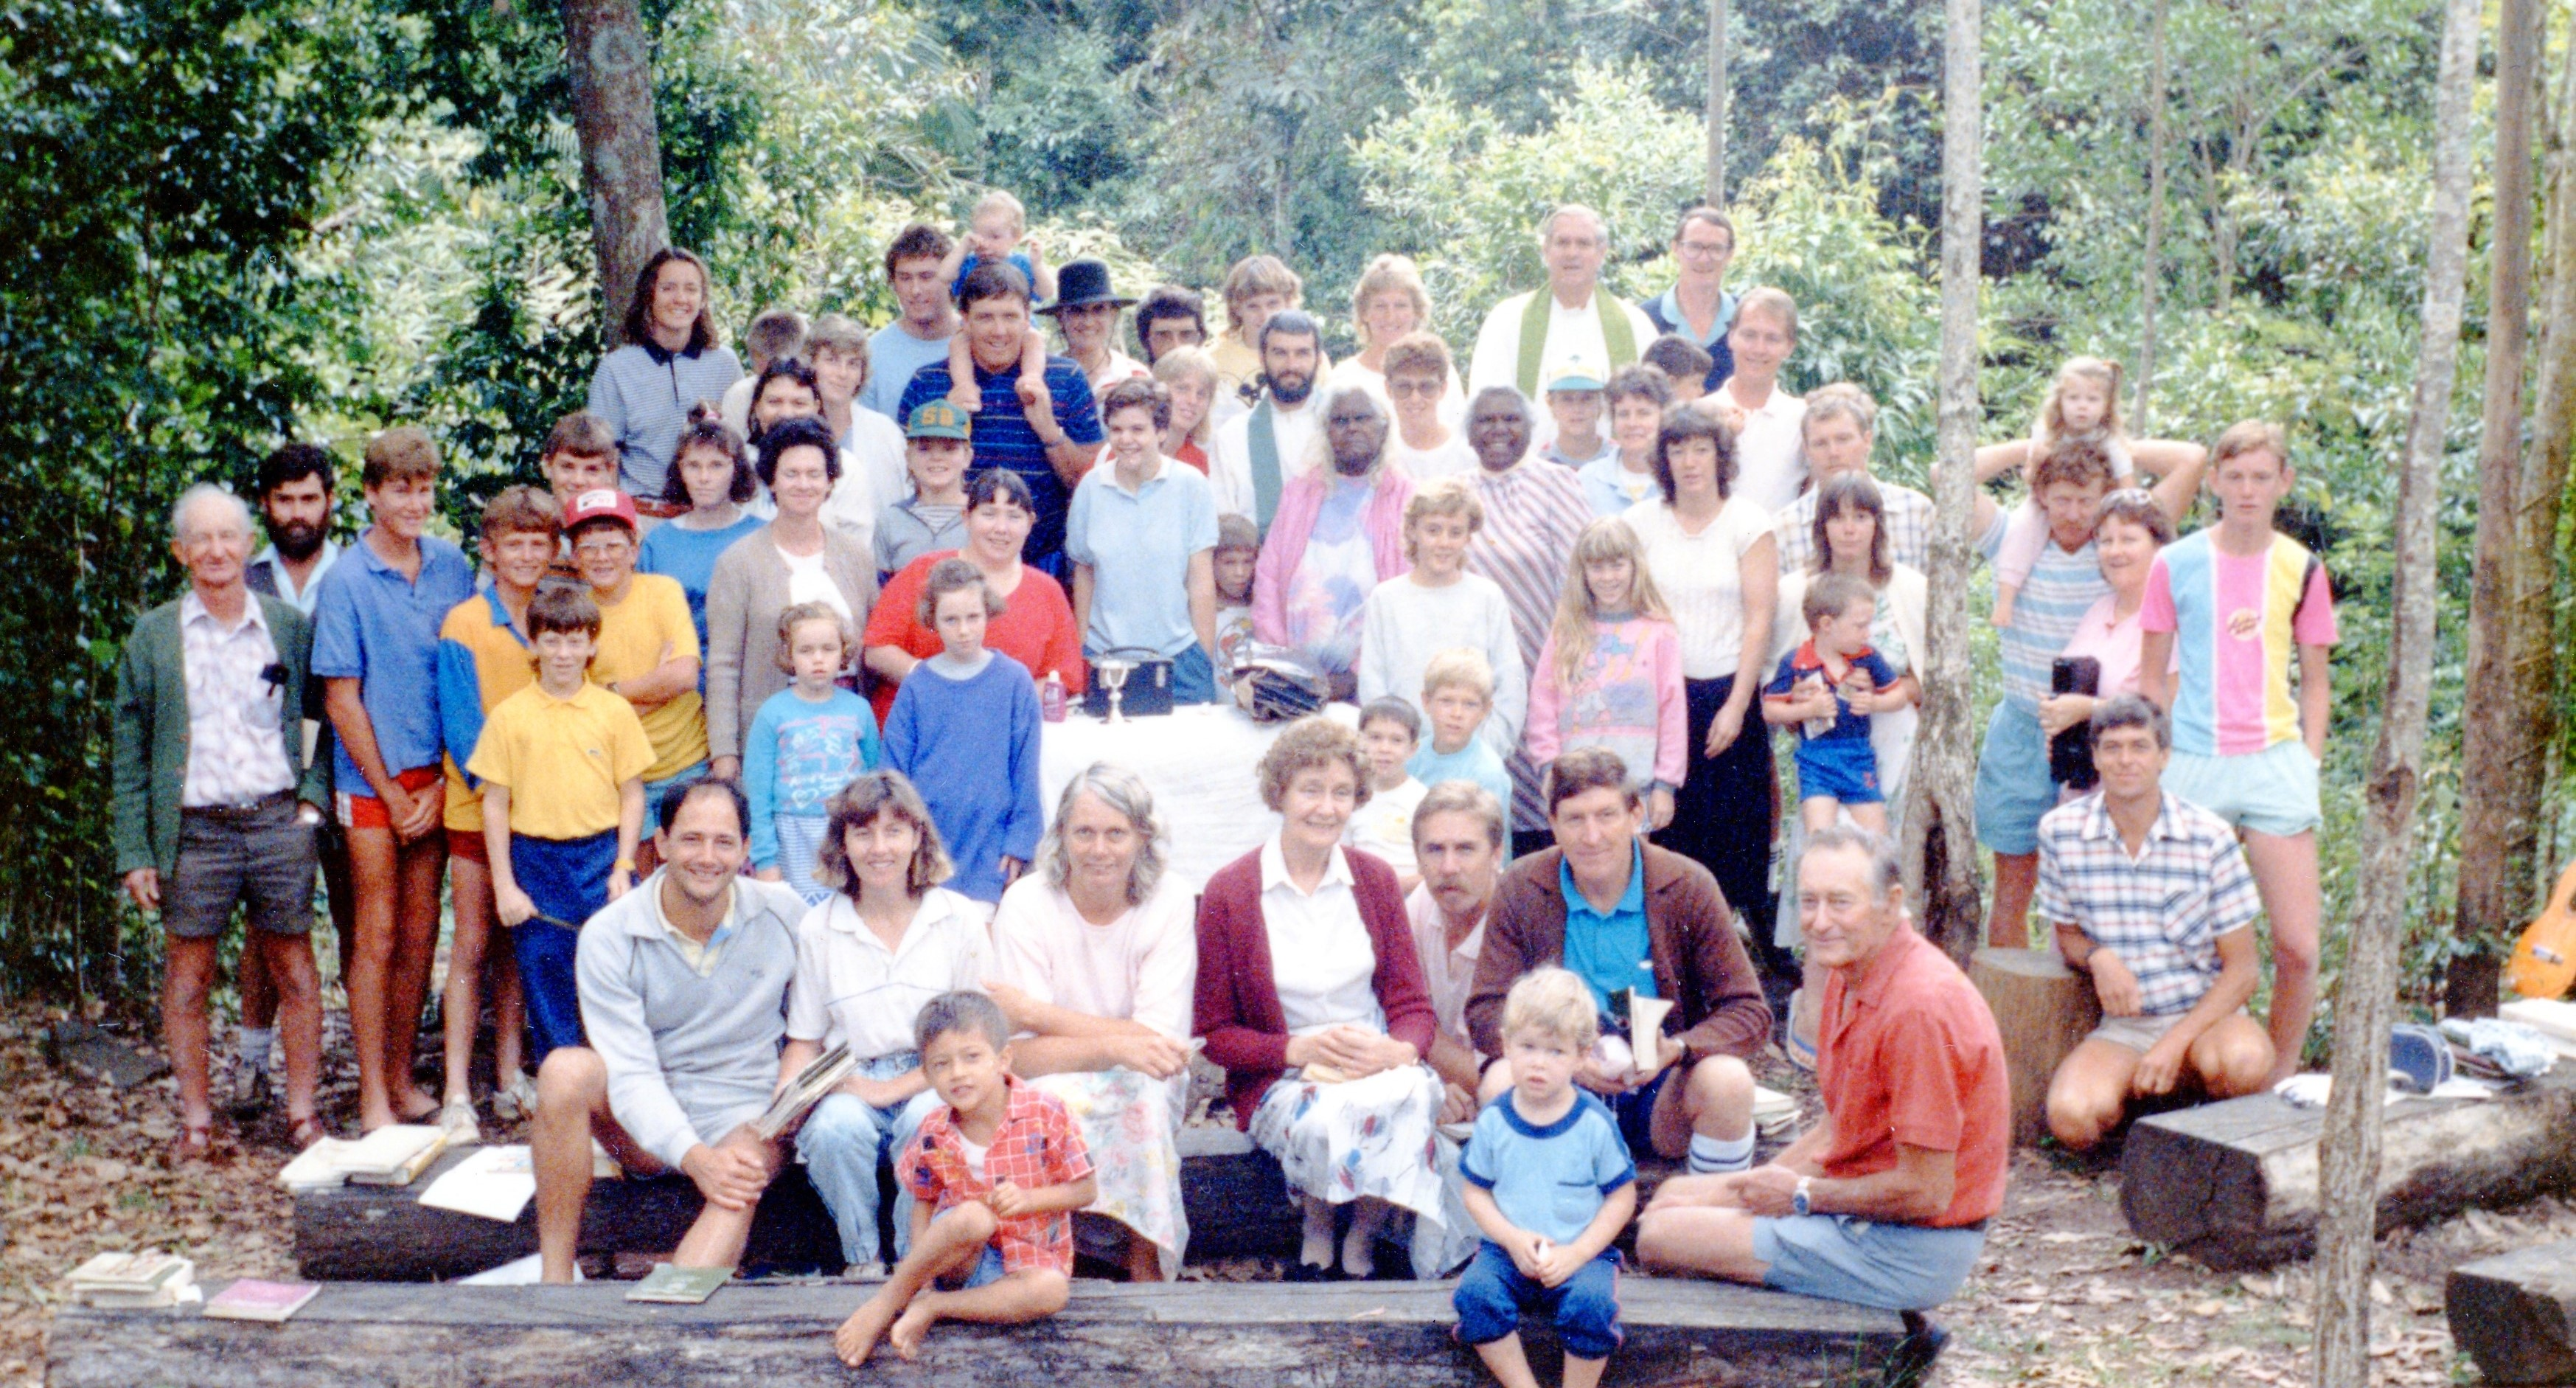
\includegraphics[width=1.\textwidth,center]{../images/bushChuchMapleton1987.jpg}
\caption{Combined Bush Church Mapleton. Vic McNamara and Glen Zimmerlee. Nov 1987.}
\end{center}
\end{figure*}


Despite all valiant efforts, debt spiralled to the point where every payment of the regular stipend became a recurring search for funds, a drain on the parish group's working funds. The Ladies Guilds have always been acknowledged for their willingness to assist physically and financially. The Murgon Ladies Guild Register of Payments from Guild funds from 23 November 1978 to 28 September 1990 documents payments directly into the parish working account of just over \$10,010 as stipend assistance with total contributions amounting to \$22,500. That amazing effort included covering shortfalls in Parish Assessment, over \$2,000 to painting projects on the rectory and the hall, \$5,000 to carpet the rectory, a new stove and a further \$500 for tank and guttering. Murgon Guild purchased 96 Hymn books - \$625.45, as well as augmenting the Organ and Car funds, contributing to Missions such as CMS and various Homes, and continuing to maintain and improve the Parish Hall facilities. The list could go on. And that was just Murgon Guild. Goomeri, Kilkivan and Boonara Guilds were also diligently and feverishly working in support.

Hindsight provides a view of changing district demographics beginning as early as the lead into the 1960s. Larger holdings to support family businesses were seen a more viable option to the smaller dairy and mixed farming holdings. Government supported acquisitions of `the-farm-next-door' and the registering of family businesses names and family trusts were seen as positive moves aiming to support rural industries and keep young people in these areas.

The period witnessed an enormous surge in the emphasis on higher education with `High Tops' being added to primary schools in Goomeri and Kilkivan thus allowing local children to achieve an education to a level equivalent to the current Year 10 without leaving home. Bus services to schools proliferated and education to Year 12 level was then also available at the existing nearby High School in Murgon. With higher educational qualifications, and the lure of a regular income, many secured off-farm employment, which took them out of the district. Tertiary study and entry into professional occupations with more lucrative and fulfilling employment became an achievable goal. Add in the de-regulation of the dairy industry, the loss of overseas markets for many primary produced items and the trend to broad-acre farming and the reality becomes clearer. Tthe situation in the area was a combination of many factors, not the least of these being changing lifestyles and aspirations, the ever-present effects of weather and decisions whose long-term consequences sometimes proved less advantageous than hoped for and expected. The church suffered along with the rest of the community.

Although always assured the salary would be found, at the expense of any other commitment, with a wife and five children to support, it is easy to see why this concerned Rev McNamara. Added to this was his very deep concern and distress that all efforts to the contrary seemed to be failing under his leadership. Rev McNamara's sincere concern for parish welfare led him to confide in his wardens that, after eleven happy years with them, he felt it was time to move on so a `new-broom' could look at the situation with fresh eyes. With their permission he began investigating the family's possible future.

He accepted the offer of Assistant Curate at St Peter's Gympie (1991-1994) where he held a Missions Chaplain role. This led to his appointment as Locum Tenens Cunnamulla (1994-1996) and then Priest in Charge - Southern Gulf. He and Doreen were very happy in their life stationed in Normanton where they remained from 1996 until his sudden passing on 20 March 2001.\footnote{Diocesan Clergy Records, p. 25}

\section{1990--1991 : Rev Gerald Greaves (Locum Tenens)}

During the interregnum Kilkivan Parish was granted the services of Rev Gerald Greaves who was living in the Kingaroy area. His previous experience as Vicar of Taroom 1971-1974; Rector of Nanango 1974-1977; Assistant to the Rector, Mt Isa 1980-1987 before moving to Kingaroy in with Permission to Officiate in the Brisbane Diocese, all combined to make him a suitable Locum Tenens for the Kilkivan parish for 1989-1991.\footnote{Diocesan Clergy Records.}

A rather shy man and reserved man at first, he reacted positively for the warm way in which he was welcomed and a rather more jovial and relaxed side was revealed. He gladly threw his efforts behind all efforts to move forward in financial terms. Rev Greaves was an avid and knowledgeable gardener. The various Guilds put this to good use, fashioning fund-raising events such as the ``Winter Green' afternoons which incorporated gardening hints, tips and demonstrations as well as the sale of plants, a sizeable proportion of which Fr Gerald donated from his supply. Fashion parades and delectable Afternoon Teas also featured.

The services roster was followed dutifully, assisted by the team of Liturgical Assistants. All churches continued to be maintained fully and pre- and post-service preparations carried out by locals so everything was in order for services to begin on time.

After leaving the Kilkivan parish, he served as Rector of Wondai 1992-1993. Also in 1993 -- Missions Chaplain plus Locum Tenens Jandowae. LT appointments throughout 1993-2000 took him to Tara, Childers, Miles, Chinchilla, Mitchell, Roma, Dalby, and Mundubbera. Rev Greaves retired in 2000 with Permission to Officiate, Brisbane Diocese.
\balance

\printendnotes[custom]
\setcounter{endnote}{0}
\chapter{Transition and Change}
\nobalance

\section{1991--1997 : Rev Bavin John Clarke}

Bavin John Clarke was ordained both Deacon and Priest during 1988 in the Diocese of North Queensland. First appointed as Deacon Assistant to St James' Cathedral, Townsville in 1988, he continued his service there as Assistant Priest (1988-1989), then as Curate/Precentor (1990-1991). He was also appointee as Chaplain -- Mission to Seamen during 1991 before moving, mid-1991 as Priest to the Parish of Kilkivan.\footnote{Clergy Records}




\begin{figure}
\begin{center}
\includegraphics[width=1.\linewidth,center]{../images/bavin.jpg}
\caption{Rev Bavin Clarke}
\end{center}
\end{figure}


Prior to his arrival Rev A J Gerlach returned to the parish to conduct Holy Communion services in the parish. The Rural Dean, Rev Wisken, of Kingaroy also filled in on occasions before the Clarkes took up residence.

Bavin John Clarke's name was brought by Bishop Clyde Wood to the attention of Parish Wardens and Parochial Nominators, I D Kapernick, E B Mcintosh and K A Batts, who subsequently interviewed him. Impressed by his voluminous file of references and recommendations they remained a little hesitant regarding his complete lack of parish experience, particularly with no rural background. Coming directly from positions within a cathedral setting he was well versed in correct and traditional `High Church' worship procedures there, which were not pursued in Kilkivan parish. With Bishop Wood's firm and insistent assurance that he was `the man for the job' in their parish, they moved to have him appointed as Priest-in-Charge for a trial period only, with no objections being raised by the Diocese. he was subsequently appointed as Rector.

Accompanied by his wife, Josephine. and family they moved into the rectory in July 1991, along with their pet dog, a Whippet -- truly a case of `dogs looking like their owners!'. He was the first priest appointed to this Anglican parish who insisted he be called `Father' not `Reverend'. This was rather strenuously objected to in some quarters, most fiercely in Kilkivan, widely known for its resistance to `high church' procedure. However, Father Bavin's service presentation and his enthusiastic positivism and drive was immediately evident and stood him in good stead. His first signature appeared in the register on 14 July 1991 beginning an almost six-year incumbency, during which time he was never seen in anything but full black attire with his clerical collar firmly in place.

His support on arrival consisted of a hard-working Parish Council and administrative team. Husband and wife Keith and Marjorie Batts accepted the positions of Synod Representatives. An average of 20 communicants each Sunday, 10 Baptisms, 15 candidates confirmed and 15 marriages are recorded.\footnote{1991 Year Book p. 78} Fr Clarke maintained the existing services roster with the minor alteration of moving Windera's Holy Communion to a one-per-month 7.00 pm service rather than the twice-per-month with one being on a week night. The programme remained stable throughout Fr Bavin's incumbency.

Confirmation services were an annual event with an ever-changing parade of Bishops. Bishop Adrian Charles confirmed 11young people 6 October 1991. As a former Rector of Wondai, he knew the district and many of the people from the Kilkivan Parish. Bishop Clyde Wood performed these Confirmation duties in November in both 1992 and 1993. In 1984 Bishop Mason officiated with the Rector's report noting Wondai `combined with us on the day'. A further group `admitted late to the course' were presented to the Archbishop in November in Kingaroy as `Fr Graheme Baldock is happy to share his service with us' -- further evidence of Fr Bavin's meticulous attention to proper presentation in all areas.\footnote{Parish of Kilkivan Minutes 1984 and arish Confirmation Register}.

At the 30 January 1994 AGM in the Parish Hall in Murgon, `Mick' Kapernick continued as Rector's Warden, Mike Gerlach and Ewen McIntosh as Peoples' Wardens and all three wardens as Parochial Nominators; Alan and Elizabeth Meizer- Synod; Kelie Wigg -- Auditor. Fr Bavin appointed Jenny Thompson as his Rector's Warden in a special position for Cherbourg. She was approved for Liturgical Assistant status. The parish council voted to support her application for admission as a deacon in Canon Lyall Turley's 19 February 1995 meeting with the Cherbourg community.

The day to day running of the parish was continuing smoothly, though funding issues grew. With the financial situation in 1994 reaching disturbing proportions, M McIntosh was reappointed unopposed as Treasurer along with Tom McAntee as Deputy Chair of the Finance Committee -- not enviable roles to carry, though computerising the finances had enhanced management as did Fr Bavin's support and ability to see opportunity in every difficulty. The office was moved from the Rectory Study into the church vestry to `assist in the mechanics of running the Parish week by week'. The Study then became more accessible for private consultations and counselling.




\begin{figure}
\begin{center}
\includegraphics[width=1.\linewidth,center]{../images/waldockGerlach.jpg}
\caption{Shirley Waldock and Shirley Gerlach}
\end{center}
\end{figure}


In 1994 the actual income received fell alarmingly to \$11,000 below the projected figure. Both the Car Account and the Curate's House rentals were accessed heavily in a `rob Peter to pay Paul' situation leaving both severely depleted and at an all-time low, simply to pay stipends and the most pressing of often long overdue accounts. Despite the stirling efforts of all guilds, fundraising events, pastoral care and youth outreach, the parish continued to slide backwards financially. Fr Bavin's report that `it was a sad but true fact that 86\%of Parishes in the Western Region are considered marginal', provided little solace or solution to the local situation, though an air of determination to progress positively remained.

Mick and Marion Kapernick donated and installed a beautiful Aumbrey in memory of family members and Harold and June Bradford generously gifted a lectern dedicated to the memory of Ian Graham Bradford, parishioner of St Peter's Cathedral, Darwin. A Memorial service for founding member of Holy Trinity church, Windera, Mrs Flo Maudsley combined with a family Baptism was a highlight of the year where `Flo's generosity with (donating) the (Windera) organ and her `deep, spiritual legacy' was acknowledged. Following the closure of Holy Trinity, the organ found a home in Christ Church, Murgon. Fr Bavin proposed two projects to honour the memory and dedication of Cherbourg elder, Nellie Sherridan -- 1. A reredos memorial in the church and 2. A Nellie Sherridan Memorial Scholarship for local Indigenous youth. Some funds were gathered but neither project reached fruition.

Seemingly, the treasurer's appraisal of the situation as being `not just \emph{tight'} but was actually \emph{critical}, had galvanized the troops into all-out efforts to rectify the imbalance. Although the fundraising efforts were many and varied, the most outstanding one was the massive `Steptoe Auction' held in the old (now demolished) Goomeri Show Pavilion. This was a huge, whole-of-parish undertaking and included almost every imaginable item, from bags of manure to bric-a-brac to antique furniture and valuable crockery. Widely promoted, it attracted buyers from all over Queensland and interstate. It was a huge financial success raising thousands of dollars, allowing the rector to report on what he described as the 1995 financial `miracle' where `we closed 1995 \ldots{} having turned a massive debt into a modest surplus.' Successful approaches to have Diocesan funding for ministry in Cherbourg reinstated also played a part, as did Fr Bavin's successful abatement of the \$2000 1994 assessment, along with the offsetting `from the Good Shepherd relief fund for the first half (of 1995)', then to be `negotiated further after the end of the financial year'.\footnote{Kilkivan Parish Council Minutes - Rectors reports -- 3 April 1995 and 22February 1996}

While support from the Good Shepherd fund was granted in 1995, the Archbishop's first preference lay with the concept of `Twinning' with a viable city parish - aimed to enhance understanding of rural situations, mutual support and fellowship -- the Good Shepherd Fund to be accessed only as a second option. Kilkivan parish was `twinned' with St Clement's on the Hill, Stafford. Their rector, Fr Keith Slater conveyed news of their immediate generosity in offering financial assistance (\$2000 to general finances plus offers to help with painting of rectory -- fellowship and general support). He felt our parish had a lot to offer them in return. This led to a long association with many visits by their Bushwalking Group, always commencing with sharing in a combined Communion service. Bushwalks, picnics, services and fellowship took many of the locals to places in the district which even they had not previously explored. Occasional reciprocal preaching Sundays also built connection and were appreciated and enlightening for both parishes.

\subsection{Parish Amalgamations Proposed}

Fr Bavin's June 1995 report also reflected on the decline in the church over the past 10 years. The Parish Council's opposition to the Age Limitations Canon was understandable in view of the ageing and ailing body of dedicated workers in a struggling rural parish as was their expressed wish for it to be rescinded. Following fruitful discussions at an Archdeaconry Conference with Bishop Wood his report outlined (emphatically emphasising they were discussion points only) some ideas put forward by `the Area Dean and one other clergy' as to a possible way forward for Bunya Deanery parishes. Reaction from Kingaroy and Crow's Nest had been `swift, sharp and uncomplimentary', with Wondai's Fr John Watlemaro reporting their growing feeling that, if any move in amalgamation was to progress, they should be linked with Kilkivan Parish. Wondai, with a very large overdraft and a rectory requiring extensive repairs, was no longer considered viable. Moving towards amalgamation seemed the only logical decision despite the inherent rivalries which existed between the two areas.

Both Kilkivan and Wondai parishes were adamant that no centres should close, meaning any new parish would have 10 operational centres, rectories and halls, all except one of wooden construction requiring costly maintenance, a distance of well over 100 kilometres between the parish's two extremities (Kilkivan and Proston), both parishes with ageing populations and failing income streams. Serious concern and misgivings were voiced. Again, Fr Bavin's `faith in God and in the future for the area' brought a calmness to discussions.

The apparent opinion of senior clergy, as presented to the two parishes, was that a combined platform would provide a wider field of potential participation and that while the problem of extended travel distances and time was recognised, a younger, vibrant person with a talent in Youth Work would be sought. While the concept of amalgamation was viewed locally as a last resort, the stark facts finally led to the realization that it was the only option now being offered. A further complication was the combining or a Parochial District and a Benefice Parish. Kilkivan Parish would lose its Benefice status should a Provisional Parish result. The ramifications of this and many other `how to proceed from here' issues required further serious investigation before any decision and agreements could by decided and agreed to in any formal way.

\subsection{Provisional Parish of Cherbourg}

While all of the above was happening, and beginning in the early part of Fr Bavin's incumbency, there were moves by the Cherbourg community to become a separate Parish under the control of Indigenous Ministries. Fr Bavin, with social justice a personal high priority, supported this concept whole-heartedly and pursued it with vigorous tenacity. An indigenous Minister, Rev Wayne Connolly from North Queensland, was appointed with sole responsibility for ministry in the proposed Provisional Parish of Cherbourg. Though remaining under the umbrella and guidance (mentoring) of Fr Bavin Clarke in Murgon and supported through the Brisbane Diocese, this altered status meant that Cherbourg was removed as a centre from Kilkivan Parish's ministry coverage. Therefore, it was not included in planning during the parish amalgamation process. Rev Connolly's incumbency was short-lived and another northern region minister\textbf{,} Rev Wayne Stafford succeeded him. He too left after a short period. In hindsight, perhaps someone from a southern, more local area may have been able to be sourced with more positive results.

Cherbourg Anglican church was granted Provisional Parish status under Rev Jenny Thompson\textbf{,} with a 5-year term to prove viability as an independent parish. All three of the above indigenous ministers were installed and commissioned with great pomp and ceremony, attended by a large contingent of Diocesan dignitaries including Archbishop Hollingworth, as well as representatives from all local church denominations and residents from the entire district and from Cherbourg town itself. Responsibility for the Cherbourg church building and its worshiping community was removed totally from Parish of Kilkivan at this time. While it went forward with full district support of its vision, this laudable venture did not continue along the envisaged path. Rev Jenny returned to live in Brisbane.

Cherbourg centre, without notice to Murgon's Rector or administration team, reverted to Kilkivan (Barambah) Parish control in 2000. Thus, no arrangements for regular services in that centre were made. Funerals were conducted by Indigenous Ministries persons who travelled to the town or by Murgon's priest or licenced Liturgical Lay persons as requested.

Efforts have since been made to re-introduce regular worship services. Regional Bishop, the Rt Rev Robert Nolan made several trips from Toowoomba for this purpose with a positive view to appointing an Indigenous Lay Minister to officiate. Sadly, these efforts did not achieve a favourable outcome, as with several later attempts by Murgon Lay persons, following local requests for the resumption of regular services, again with the common view of fostering the appointing local Cherbourg residents to become actively involved in providing church services. The once beautiful and revered building with its locally carved and decorated altar and communion rails was badly disrespected and subsequently fell into disrepair. A further complication emerged when it was discovered that the building had been erected on leased land. Since the tenure of the lease had concluded with renewal not possible, disappointingly, Bishop Cameron Venables was left with no option. Holy Spirit Church, Cherbourg has been officially as a place of Anglican worship in the community.

\subsection{Progress into Amalgamation}

Following a couple of years of seeming endless local individual and combined meetings and sometimes heated discussions, interspersed with consultations with Diocesan personnel, most of the basic points of agreement seemed to have been reached during combined meetings of Churchwardens in the presence Fr John Watlemaro. Subsequently discussed, clarified and endorsed under the direction of Fr John and Fr Bavin, these emerged as follows:

\begin{enumerate}
\def\labelenumi{\arabic{enumi}.}
\item
  A completely new Parish be created with its own identity.
\item
  The spiritual/management centre of the new Parish to be based at Murgon due to:
\end{enumerate}

\begin{enumerate}
\def\labelenumi{(\alph{enumi})}
\item
  Its geographical location in the centre of the new parish.
\item
  Its Rectory is currently up to standard or would be so with minimal expenditure.
\end{enumerate}

\begin{enumerate}
\def\labelenumi{\arabic{enumi}.}
\setcounter{enumi}{2}
\item
  The current centres of worship be retained intact.
\item
  The current residences in Wondai and Murgon not being required as a Vicarage and Curatage respectively, continue to be rented.
\item
  A possible future Parish Council (decided at a special general meeting):
\end{enumerate}

\begin{quote}
Two elected Churchwardens.

One priest's Churchwarden (appointed by the priest)

Two District Churchwardens for each centre with one elected and one appointed as per above.

A Pastoral Contact Person for each centre may be nominated separately or from the list above.
\end{quote}

\begin{enumerate}
\def\labelenumi{\arabic{enumi}.}
\setcounter{enumi}{5}
\item
  The current Ladies Guilds are to remain intact.
\end{enumerate}

The above information was to be sent to Bishop Wood for summation and direction.\footnote{Agenda Paper -- Amalgamation, to be presented at a combined parishes' meeting in Murgon at 7.00 pm on 21 March 1996} The consensus was that the new entity be named the Provisional Barambah of Barambah. A point was reached where a `to be or not to be' decision needed to be made. 1 July 1996 was set down as Decision Day when all parties would sign off on the meeting's outcome. Under Diocesan policy, should amalgamation proceed, then both present clergy persons should move. This was relatively easy for Rev Watlemaro as Vicar of a Parochial District and he left Wondai without complication and Fr Bavin undertook the added caretaker duties to Wondai.

Kilkivan Parish could not retain Benefice status following a merger with a Parochial District, though it would retain Parish status in the interim. In April 1996, Benefice status was officially removed, allowing progress towards the official recognition of the proposed title - Provisional Parish of Barambah. Fr Bavin retained his `Rector' title though this would not be the case for an incoming priest.

Illness and accidents interspersed and interrupted the smooth running of Kilkivan Parish several times during this 1991-1996. At one point two parish wardens, were seriously ill at the same time, leaving just one Peoples' Warden and the Priest to shoulder the load. Both recovered. Though Rector's Warden Mick Kapernick returned to duty, Peoples' Warden, E McIntosh, resigned from his Warden's role and as a Liturgical Assistant.

Father Bavin himself had to contend with two periods of illness requiring at least two weeks recovery time and then bereavement on the passing of his father. Further, a car accident on the way to a Film Evening in aid of Missions at Boonara left both he and Josephine bruised and suffering whip-lash injuries, though nothing more serious, and what he described as `an embarrassing disagreement with the Hall steps.' Throughout, he retained his smile and cheery outlook while seeking a personal way forward upon departure.

Fr Bavin Clarke's six years in the Parish of Kilkivan could be described as, eventful, exhausting, filled with a roller-coaster ride of alternating parish highs and lows, and always interesting. The Murgon Guild `s record of Income and Expenditure (1991-2013) notes the 23 January 1997 `purchase of gift for the Clarkes.' At the Parish's farewell event Fr Bavin and Josephine were sincerely thanked for their combined commitment to the welfare of the entire parish and extending well beyond its original boundaries and into the mission fields overseas. Josephine's involvement in multiple organizations and son Andrew's commitment to Youth activities were also recognized. His gracious reply acknowledged the `above and beyond' assistance he had received and wished the area success in their `new-parish future'.

The Clarke family moved to Thornlands, Brisbane where he took a position a Chaplain QIT from 1997. Fr Bavin Clarke was received into the Roman Catholic Church in 2002. Clergy notes.

\section{1998--2002: Rev Norman William Wagstaff}

1997 was another year where the area was without an incumbent priest, this time with two parishes involved and still striving to finalize amalgamation details. Worshipers were grateful for the generosity of various clergy who visited to deliver the sacraments and for the Liturgical Assistants who continued with Morning and Evening Prayer services. Rev AJ Gerlach returned to provided Holy Communion over the weekend of 14 February and Fr Tom Hood's signature accompanies details of Holy Communion services up to 26 April 1997.\footnote{Parish of Kilkivan Services Register from Windera centre}

In 1996 Bishop Raymond Smith succeeded Bishop Clyde Wood in the Western Region and stepped into the fraught process of unravelling two parishes and successfully tying them into one. The critical points for successful transfer into a spiritually, financially viable and cohesive entity required wise decisions from the inception. Reverend Norman William Wagstaff was introduced to a special evening meeting of combined congregations from both Kilkivan and Wondai parishes early in 1997. He presented with an extensive background of service in the more remote, western rural areas of Queensland. A St Francis' College, Brisbane graduate, he was ordained Deacon 1975 and Priested in 1976. He served in the Diocese of Rockhampton from 1977 to 1993, moving through Barcaldine, Moranbah, Mt Morgan and The Barcoo as well as using his talents in Chaplaincy positions in Geriatric Institutions and the Rockhampton Hospital with these duties overlapping his Rectors role in at least two of his parishes. His move into the Diocese of Brisbane commenced with his 1993-1997 appointment as Rector, St Peter's Millmerran with the later addition of Missions Chaplain added.\footnote{Diocese of Brisbane, Clergy Records}

This record of experience led Bishop Smith and others senior clergy responsible for parish appointments to believe Fr Norman was a suitable contender, though not conforming to their original stated `ideal' for the area. An older man than originally envisaged by the locals, Fr Norman was also a widower and not a well man. Any `misgivings' were as much for his personal welfare as for the parish's future. Five years later he openly revealed that he originally shared similar feelings. He came to Murgon with his big dog -- another case of `dogs and their owners\ldots'and from 3 May 1997, his signature accompanied service register entries.

Fr Norman began as Priest in Charge of Kilkivan Parish and Locum Tenens to Wondai. From 1998 the ensuing parish was named in Diocesan records as the Provisional Parish of Barambah with Fr Norman as Priest in Charge\textbf{.} Adding the centres of Wondai, Mondure, Proston and Hivesville to Kilkivan Parish's Windera, Goomeri, Kilkivan, Boonara and Murgon was, from the start, and over-optimistic endeavour even with an extensive team of liturgical assistants working diligently and providing services in all centres.\footnote{Diocesan Correspondence Files 1998} While the enormity of the task ahead seemed to have required a younger man, Fr Norman to his credit, threw himself willingly and with determination, into dealing with the demands which presented.

Fr Norman was very grateful for the strong support and friendship given him by Allan and Elizabeth Meizer who were the Synod representatives when he arrived. They were also Parish Wardens along with Tom McAntee. Mrs Meizer also acted as Office Manager. There was a slight `changing of the guard' during 1998 with A Meizer, T McAntee and CE Weier accepting nominations as Wardens. Mrs P Hansen and P Phipps were endorsed as Synod representatives. Mrs K M Schmidhauser is also included later. The number of communicants per week remained around 43 but a decline to one Baptism, one Marriage and no Admissions to Communion or Confirmations, was noted with concern.\footnote{1998 Year Book p. 72} The names listed above show a very positive and pleasing spirit of co-operation between the two former parish congregations.

The 1999 Year Book p. 96 has a listing for Kilkivan with the notation `Refer Barambah'. Thankfully, numbers again increased with the p.83 entry in the 1999 year book showing Barambah Parish with 52 weekly communicants, 11 Baptism and five Marriages. Funerals seem to have remained steady at around seven per year. Although Rev Wagstaff approached the task with positivity, health issues with his lungs impeded his efforts. The only concerning point in the Murgon centre was the appearance of a rift developing between the priest and the organist -- both strongly determined personalities.

On several occasions over his incumbency, illness forced periods of leave, during which times the parish was very grateful for services conducted by visiting clergy. Rev Gerlach came again, Bishop Smith stood in on occasions, Rev W J Pimson acted as Locum Tenens for a period in 1999, and Rev Libby Crossman (Kingaroy) officiated in June 2000. The services in all centres continued at scheduled times but if a clergy person was not available on a day where Holy Communion services were to be celebrated Lay persons offered Prayer and Worship services.

The Mothers Union Thanksgiving Service and Holy Eucharist, a firmly entrenched feature in Murgon's calendar, was celebrated on 5 October 2001 with Fr Norman celebrating. Guest from other Deanery centres boosted attendance to 46 with 42 receiving the sacrament.\footnote{Parish Services Register}

Even health problems can bring unexpected positive results. God does move in mysterious ways! Fr Norman's association with hospitals brought him into contact with the local Director of Nursing and `love blossomed' into marriage. His new wife, Gwenn, can be credited with paving the way for a different regime of treatment for his lung condition which made his life easier, at least on the health front, with hospitalization less frequent.

During this 1997-2002 period, despite all the efforts put into improving attendance and participation in the prospective broader, `combined platform (which) would provide a wider field of potential participation', and the hoped for `increase in youth participation', neither eventuated. The ageing and ailing workers became more so and decreased in number while the problem of extended travel distances and time remained even though road conditions~vehicle comfort and reliability both improved markedly. These brought altered focus and aspirations on how the weekends were spent. Where once school teachers and bank and other business employees joined the local sports clubs, the lure of sun and surf of families in the cities meant this no longer happened. Junior sport burgeoned with interest stirred by televised state, national and international competitions and so the story continued.

Along with changing focus to a more secular approach to daily living and societal values, faith in God receded from the prominence in which the early Murgon settlers held it. All the honest and concerted efforts in the area did not achieve all the hoped-for outcomes.~No blame for this can be laid on any one person or group. Fr Norman and the peoples of the church worked tirelessly to achieve the hoped-for goals. The burden was shared and sale of the rectory building in Wondai and the curate's house in Murgon made a substantial contribution to the project. The decision to sell these properties was very difficult but ultimately helped the parish greatly by reducing the ongoing maintenance, repair and renovation costs thereby allaying some of the immediate financial pressure. All in all, it was a trying and distressing time for all and for Fr Norman in particular.

Canon Ron Dyson in his 2014 communications, commented on a three-week stay in the parish in 2002. He begins by recalling happy memories of his time there, adding: `\emph{The Rector in 2002, Fr Norman Wagstaff, was not in good health and I was asked by Archdeacon Irvine Scott (Appointee of locums) to travel to Murgon and assist Fr Wagstaff\ldots who stayed on the Rectory for the period. I was accommodated in a B\&B run by Greg and Judy Wilson on the Goomeri Road for those three weeks.}'\footnote{2014 Correspondence from Canon Ron Dyson}

Fr Norman, his health still less than satisfactory, retired from the parish and from full-time ministry in 2002. He and Gwynn were farewelled in his last service as Priest in Charge of the Parish of Barambah, conducted in Christ Church Murgon on 21 July 2002 where he presided over a Holy Eucharist with 92 people present, including members of Fr Norman's family. A lovely luncheon, fellowship and speeches followed in the Parish Hall. The 2002 Year Book, p 78 lists Barambah Parish as vacant. Wardens, who carried on were M G McIntosh, S Waldock (both also L As) and C Weier: Synod representatives were P N Hansen and B R Hockey, also a L A, as were Jim and Linda Quinn, Allan Meizer.

Fr Norman and Gwynn moved to Carlyle Gardens Retirement Village in Bargara, enjoying a happy retirement by the sea. He has continued part-time work in the Bundaberg Parish -- mainly in Bargara. He is greatly valued and respected by the people in Carlyle Gardens and in church circles in the Bundaberg Parish as a whole.

No full-time minister has been employed in Barambah Parish since 2002, though services continued to be conducted by the team of lay assistants with some visiting clergy assistance.
\balance

\printendnotes[custom]
\setcounter{endnote}{0}
\chapter{More Troubled Times}
\nobalance

\section{2002/- : No resident priest}

At the time of writing, no full-time resident Priest has been incumbent in the Parish for the 18 years since 2002. During the 2002/2003 period the idea of a United Ministries District run from Kingaroy was again put forward. Initially, Nanango and Barambah parishes were mooted as being included under Kingaroy's Rev Geoffrey Bradford, with two assistant clergy persons to be appointed. Kingaroy Parish was to continue to operate without major change under this arrangement. However, Nanango parish resisted strongly and were not included. In the face of local misgivings along with prayers for success, the proposal was eventually trialled. However, the initially proposed `assisting clergy' appointments were not made. Nor were any adjustments made to the number of added centres to receive his care. A central line for a `run' through the major Barambah Parish towns was introduced and scheduled to follow on from his Kingaroy duties. Nearby country centres were encouraged to attend these services.

This venture proved an arduous, impossible task for one man, including as it did, the overseeing of administrative duties for the whole area. Mr Rod Foster who joined the Murgon church in 2002 and immediately became an active participant. Fr Geoffrey interviewed him as a prospective Liturgical Assistant for the area and he was successfully installed in the position, under a general lay-reader's licence with the addition of permission to officiated at funerals -- a great boost to the provision of all services.

The travelling time between centres from Kingaroy to Kilkivan meant that scheduled services were usually started by the rostered lay person and often progressed to the gradual hymn before the priest's hurried and fully gowned arrival. Bishop Raymond Smith once stood in for Fr Geoffrey. His only comment to us on the situation was a concerned and sad shake-of-the head. Very quickly, serious effects on Fr Geoffrey's health and life in general became apparent, leading to his early departure. This was a serious consequence for the Kingaroy Parish itself, and, in turn, led to the early 2003 abandonment of the concept.

In early May 2003, Canon Ron Dyson, who had visited briefly in 2002, took up a much-welcomed three-month Locumship. Further signatures of persons who assisted through the period included DR Snape and Br Lionel, S James and Bishop Smith.

\section{2003--2005 : Fr John Pryce-Davies (Locum Tenens)}

Through the efforts of the Western Region's Bishop, Fr John Pryce-Davies, then living in Redcliffe, was approached and accepted a 3 days/week Locum Tenens/ Priest-in-Charge position in Barambah, beginning in October 2003. The parish offered him the use of the parish car to travel to and from his home, all costs covered, in addition to parish usage. The Liturgical Assistants from the various and distanced centres were brought together in regular training and discussion gatherings with many forward steps resulting. A greater sense of cohesion was restored. It was an eventful and co-operative period where some very hard decisions in the parish were taken and acted upon.




\begin{figure*}[!htb]
\begin{center}
\includegraphics[width=1.\textwidth,center]{../images/aspinall2006.jpg}
\caption{(l to r) Jim Quinn, Linda Quinn, Fr Stuart James, Abp Aspinall, LAs Allan Meizer, Marcia McIntosh, Barbara Hockey, Shirley Waldock. 3rd March 2006}
\end{center}
\end{figure*}


\section{The Vann Estate and Lay Ministry}

As soon as he arrived Fr John Pryce-Davies saw the need for greater pastoral care in the area and began discussions with Bishop Nolan (Western Region) to address this. A former Murgon resident and parishioner, George Vann, had bequeathed a very large sum of money to the Diocese specifically for provision of care for the elderly in Murgon several years before. Although some tentative enquiries had been made during Fr Bavin Clarke's time, nothing had progressed. Fr John and Bishop Nolan took this up again and took the first step forward with the idea of appointing a Lay Minister with special focus on pastoral care. In due course, with full Diocesan approval, Mrs Marcia McIntosh was appointed to the position in a special service of commissioning on 29 May, 2004, a position which she held until the Parish AGM 28 February 2015. Although this was an honorary lay position, a sum of \$100/week was provided through funds set aside from the Vann Estate monies to cover some running and sundry expenses for the task during the period of commissioned service.




\begin{figure*}[!htb]
\begin{center}
\includegraphics[width=1.\textwidth,center]{../images/openingGeorgeVannMemorialUnits.jpg}
\caption{Opening the George Vann Memorial Units. 18\textsuperscript{th} January 2012, (l to r) ?, Fr Rod McDonald, ?, The Most Reverend Archbishop and Primate Of Australia, Lay Minister Marcia McIntosh}
\end{center}
\end{figure*}


On the Commissioning day, Bishop Nolan and the congregation took the opportunity to bury with reverence, George Vann's ashes in the church's garden area.

Continuing investigations revealed that the local interests and those of the Diocese were on majorly divergent paths. Local understanding was that monies were to be used in Murgon for Murgon residents, while Diocesan interpretation saw it more broadly as `for use in the provision of care for Murgon residents' and plans were in the formative stage for the bequest to be applied to facilities in Hervey Bay, considered to be regionally `for Murgon'. This brought swift and distressed reactions from the local people. The two-plus-hours travel time each way by road was cited along with the lack of bus or train connections and the splitting of elderly couples should one require care. Credit must be given to Bishop Nolan, Fr John Pryce-Davies and those motivated parishioners who wrote and strenuously voiced these concerns and brought the project into what became a protracted discussion process.

Fr Pryce-Davies relinquished his locum position during 2005. While his regular Holy Communion services and his wise guidance were greatly missed, the travel and family ties influencing his decision were understood. Apart from his interest in seeking action on the Van Estate and his part in establishing Lay Ministry, his term of office brought other significant changes in the area, namely two church closures.




\begin{figure*}[!htb]
\begin{center}
\includegraphics[width=1.\textwidth,center]{../images/nolanGoomeri2006.jpg}
\caption{Goomeri 90\textsuperscript{th} Anniversary, 2006. Canon Ron Dyson, Fr Norman Wagstaff, Bishop Rob Nolan, Fr Trevor Cichero.}
\end{center}
\end{figure*}


\section{Windera and Hivesville Churches Close}

\textbf{Church Closures}

Always very hard and emotional decisions surround the closure of church centres. On 31 May 2005, it was Bishop Nolan's sad duty to oversee the closure of Holy Trinity, Windera and Holy Spirit, Hivesville. The properties were disposed of during that year. The Windera church building, still in very sound condition, after 47 years as a church found a new life and a new role as the Library building at Cloyna State School. The Hivesville church was gifted to the Murgon Shire Council and moved to the Murgon Dairy Museum and Historical Complex. Now beautifully restored, it stands and serves as a Chapel for funerals, memorials and weddings.

Several most welcome retired priests continued to fill the void with occasional short stays and joyously welcomed. Some became very dear friends over many following years, not least of these being the late Canon Ron Dyson who ministered in extended blocks of up to six weeks and the ever- reliable Fr Stuart James who officiated at the 2005 Christmas Day Eucharist. It was a busy time for the lay assistants A Meizer, S Waldock, R Foster, M McIntosh, J and L Quinn. Fiona McFarlane's assistance by introducing and running with a ``Grow Your Faith' evening programme proved was a successful venture along Sunday School lines where parents attended along with their children.

\section{2007 : Rev Fang Ling Liaw Quested}

Rev Fang Ling Quested, a newly ordained priest resident in the neighbouring parish of Nanango where her husband Michael was rector, accepted a 3 days/week position in Barambah parish from 7 February where the parish car was again provided for travelling to and from as well as within the parish -- all costs covered.

Negotiations continued regarding the Van Estate project. Rev Fang Ling chaired a meeting on 4 September 2006 where Peter Pearce, General Manager, Direction and Development for the Diocese, where the concept of low-cost units or duplexes was affirmed, along the style of The Laurels complex in Wonda. The number of units would depend on style, Shire Council requirements and cost of land. The existing Castra Retirement Complex was on the market and Mr Pearce advised that the Diocesan care arm, Spiritus, was putting in an offer to take over control of the complex along with a proposal to construct units on adjacent land. Other options cited were land opposite the Murgon Hospital in Nutt Street or vacant Railway land in the town. P Hansen, L Steele, D Hindley, R Foster, S Waldock and M McIntosh were elected as a steering committee to format a proposal including information re type of units required and the names of possible architects and builders. A more radical proposal of using existing church land involving removal of the Rectory, Church Hall and part of the Church then erecting six or seven units in an L-shape and adding a new Function/Meeting room received consideration but was eventually shelved.

Rev Fang Ling's short seven-month stay was a time of turbulence for her in spite of her prayerful and dedicated efforts. The ageing population seemed to find her accent difficult to contend with and there were some personality clashes with a few unsympathetic and out-spoken parishioners. During this time one of her young children experienced serious health problems which, added to these other stresses, led her decision to resign the position, effective 30 September, 2007. Though only a very short-lived period, Ref Fang Ling's stay proved interesting and eventful and paved the way for a number of future developments in the life of the church.

Rev Fang Ling's departure meant Barambah Parish was again under Lay Ministry with Clergy visits interspersed throughout the following years. Judy Roberts joined the Liturgical Assistants team providing great assistance, especially to Kilkivan with her youth work there and in taking services. Rev Don Campbell returned for an Easter III service in 2010 and Canon Dyson assisted many times with often extended stays. Fr Geoffrey Reader's visits became a much anticipated and spiritually nourishing time.

Christ Church turns 90.

Christ Church Murgon celebrated the 90\textsuperscript{th} Anniversary with the Right Reverend Robert Nolan, Western Regional Bishop, presiding and preaching at a 9 May Eucharist at 3.30 pm.

A sumptuous and scrumptious repast (thought titled `light refreshments) followed in the hall. The evening was rounded off with delightful entertainment which included: amusing Skits, a Fashion Parade including vintage and current garments, modelled by congregation members from across the parish. Some unique modelling presentations kept the atmosphere light and full of happy laughter. None present would ever forget Boonara's Alice Stumm. A display of Bridal Gowns was organized by Shirley Waldock.

\section{Closure St Matthew's Church Kilkivan}

St Matthew's Church Kilkivan closed its doors after 125 years. The property was sold to Gympie Regional Council in 2014. Many church wardens and parish councillors and other valued volunteers had their spiritual roots in Kilkivan. The empty building still stands on the site fronting the highway.

\section{2012--2014 : Rev Rhonda Hunt}

Rev Rhonda Hunt - travelled from Kingaroy to serve as a non-stipended part-time minister in Barambah Parish. Her assistance in providing for the sacraments of Baptism and Marriage were valued and appreciated as well as her involvement in the regular distribution of Holy Communion to the various centres, though mainly restricted to Wondai and Murgon. The two retirement homes in the area -- Castra in Murgon and Wondai's Forest View continued to receive regular pastoral visits and the reserved sacrament by M McIntosh and J and L Quinn.

While it had seemed an endless period of machinations, a compromise was reached. Approximately \$1.5 million in a fund from the bequest was offered to construct a block of affordably priced Independent Living Units for the elderly in Murgon town. Architects, Martin Building Design were contracted along with local builder, Adrian Ramke of ARK Builders. The official opening took place on 18 March 2012.

\section{Closure St Peter's Church, Proston}

St Peter's Church, Proston, officially closed on Saturday, 14th November, 2015

The following article is from the last ever printed Focus re the relocation of the remains of benefactor Charles Shepherd from beneath the church.

The late Eric Cridland was pall-bearer when Shepheds remains were moved from Proston Cemetery for burial beneath the Church building during its construction. All Proston Anglican church property has now been sold and the church building itself has begun its new life as a private residence.

2015 Onwards

Following the retirement of the Lay Minister at the AGM in February 1915 the Parish has been visited once a month by Clergy who have volunteered their services to the Brisbane Diocese's Western Region. The burden of administration duties has fallen heavily on the shoulders of Donna Hindley and Lynda Steele since then, with, in recent times, assistance from Warden and LA, Julie Lobwein. Many thanks to these volunteers and to the Ministers who provide the sacrament of Holy Communion, originally at Wondai and Murgon for those who can make their way to these centres though later Goomeri and Boonara were given an occasional service in place of the Murgon one. Sadly, even this minimal ministry was curtailed during the Covid-19 pandemic with devastating effects on an already severely depleted congregational base. Baptisms are generally arranged to coincide with these visits with prior interviews and book-work carried out by competent volunteer assistants. Confirmation lessons which were offered by the Liturgical Assistants as the need arose have disappeared from the calendar. Funerals have been conducted by invited clergy or celebrants, including the former Lay Minister to the present time. With the inescapable reality of increasing age, disability and deaths, even the LA base has been depleted to three -- none resident in Murgon.

The Reserved Sacrament, once a valued service extended to residents of two district nursing homes -- Castra in Murgon and Forest View in Wondai -- to the sick and shut-ins throughout the Parish and in the Hospitals by those LAs who are so licenced has followed this downward trend and were suspended, due to government regulations, for the major part of 2020. Funerals became occasional COVID 19 restricted affairs with few allowed to attend, conducted by licenced LAs, invited Clergy, or other persons as approved by the Western Region Bishop, Cameron Venables, occasionally in the church buildings but more often at the Kingaroy Crematorium chapel or as graveside events.

Parish members are extremely grateful for the ministries of members of the Clergy who have visited

and provided Holy Communion and spiritual nourishment over these past years, including, among

others, who provided short term assistance: Archdeacon Tom Hood, Canon Ron Dyson, Rev Stuart James, Fr Gerald Greaves, Rev John Pinson, Fr Geoffrey Reeder. Fr Tom Hall and the Achor ministries team\emph{.} Sadly, several of these special people and at least two former Rectors have passed away in recent times. However, the memory and the benefits of their ministries remain with the communities of Barambah Parish.
\balance

\chapter{Some Prominent Anglican Citizens}
\nobalance

\section{Bernard Ashmead (Bill) Gedge}

While a great many people have offered selfless service, which could justly be researched and recorded here, Bill's passing from this earthly life in 2006 seems to have provided a fitting niche in which to include this small tribute of Bill Gedge and his loved wife, May, as a clear and encompassing examples of unstinting devotion and tireless service of the many, to the Murgon church and, indeed, to the whole parish.

Throughout many decades Bill Gedge and May's, names appeared regularly in all facets of the life of the parish. Bill, as he was dubbed in true Aussie style, sailed from England and arrived in Sydney late in his teenage years. He soon moved to Casino where he worked on a farm and met and married Ethel \underline{May} Oliver. After dairy farming there, May's asthma necessitated a change of climate and a move with the family of three to Murgon in Queensland eventuated. He purchased a Carrying business for farm produce and cream for the local Butter factory.




\begin{figure}
\begin{center}
\includegraphics[width=1.\linewidth,center]{../images/gedgeSundaySchool.jpg}
\caption{Mr Gedge at Sunday School}
\end{center}
\end{figure}


He put his expert and much-loved driving experience to weekend use, escorting the procession of rectors through the years around the parish, firstly introducing them to the routine and to the differing congregations, or simply accompanying and/or assisting them on Sunday duties, always leading the hymns with `enthusiasm and vigour', with or without musical accompaniment.

On arrival in Murgon, Bill made contact with the local church, and volunteered assistance. Lawn mowing immediately drew Bill's regular `spare time' attention and lasted until his Youth Group started having BBQs! He did not wish to see what this activity might do to `his lawns'! Some hip and knee problems also contributed.

The Gedges `green thumbs' produced fresh and preserved goods which positively influenced church finances through Guild coffers. A substantial portion of the cost of the Church Hall came from the accumulated proceeds of such sale items. In spite of a stiff leg and eventual use of two sticks to assist walking causing some angst, Bill determinately continued the ever-present maintenance work on buildings, including external painting of the church.

`The loss of May in 1968 with an asthma attack combined with an underlying heart problem left Bill without his best mate and support.' He sold his house and extensive garden and moved into a flat. Problem! No Garden! Two amusing anecdotes are worthy of the telling:

Bill's great mate, Mick Kapernick, `arrived home from work one day to find the areas between his driveway tracks dug up and planted with vegies.' Mick and Marion's son Brett clearly recalls the incident and the Kapenick family's quick reaction of the offer of their spare allotment:

\emph{`\ldots he utilised our spare allotment (where he) managed to dig the ground, grow and harvest the vegetables - even with two artificial hips and a knee. I remember quite fondly the sound of him with his crutches.'}

The move to cultivating the Kapernick's allotment leads to the second anecdote:

\emph{One day, in his `allotment garden/farm', his stiff legs caused him to overbalance into his wheelbarrow where he was stuck, in the hot sun, for a couple of hours. Passers-by happily waved cheerfully to him, blissfully unaware that it was a predicament, not just a rest period, and he waved back. Eventually, and thankfully, he was rescued.}

Bill and May were devoted members of the Murgon Anglican Church and its needs were always a priority in their lives with lay preaching, parish council, office bearing position also featuring in Bill's diary while May's support was directed to more support of Mothers Union and Guild activities. Bill was a frequent preacher at Cherbourg and he always took a box of fresh vegetables with him to share there. He was found deceased behind the wheel of his car, carefully parked in his own garage not long after having been shopping in Murgon's main street. A very fitting tribute to (Bill) Bernard Ashmead Gedge was vegetables instead of flowers to decorate the `his' Christ Church for his funeral.\footnote{Information courtesy Lurline Gedge, Edith Duthie and Brett Kapernick.}

\section{Krebs Family}

John (Jack) Krebs, a carpenter arrived in Murgon in 1919 as Christ Church was being constructed. He gained employment with builder, Herman Kratzmann. He quickly established his own building contracting business and also operated as the local funeral director. Many homes in Murgon and surrounding areas are attributed to him as well as others structures such as the Uniting Church and the Motel attached to the then Tiernan-owned Australian Hotel.

Mr Krebs was deeply involved in public life and has been described as having `lived for Murgon'. He became active in the local cricket and rugby league and earned an enviable reputation there, being awarded life membership of the Murgon Cricket Club. He was involved with Murgon's Show Society and as a poultry fancier and often exhibited his prize-winning birds locally and further afield. His service to his community covered support of the local Church of England and public service bodies such as the Hospital Board and the Fire Brigade.

He is credited as being one of the longest serving members of the Murgon Shire Council. First elected to the council in 1943, he became Shire Chairman in 1954, an office he retained for 18 years until his retirement in 1972. During his term of office many public amenities were established, including most prominently, the Jubilee Swimming Pool, the sewerage scheme and the new Council Chambers.

He was honoured with an OBE in 1973 for his services to the community and is also etched into Murgon's history by the naming of a bridge and a street in his honour. The choice of site for the Van Memorial Units in Krebs Street is, in itself, a significant. John Krebs died in 1981, was cremated at Albany Creek, and his ashes rest in the Columbarium Wall, Murgon Cemetery. His wife and one son, Darcy predeceased him.

The Krebs family is a worthy example of `families working together and staying together'. While all the Krebs enterprises were family partnerships, in 1958 they `branched out' and under the leadership of son Cliff, established and operated the Hardware and Rural Supplies store of `J Krebs and Sons' which served the whole Murgon district for decades. All of the Krebs enterprises were operated as family partnerships which included six sons, and four daughters (Stanley, Hazel, Eric, Selwyn, Darcy, Leslie, Dulcie, Phyllis and twins Clifford and Mona) and their respective families. Hazel, Mona and Les originally joined Cliff but later, as age caught up with them, other members also became involved in `the shop' as did succeeding generations The business continues as Murgon's Mitre 10 store.

The Krebs family have figured prominently in the history of Murgon town. Their contribution to Christ Church Murgon has been recognized with pews and plaques in the church. All followed in their father's footsteps of generosity to the church, community involvement in sport, particularly cricket, the Town Band, (Stanley was a member of the 47\textsuperscript{th} Battalion Band), and Show Society. Cliff was recognized as a prominent poultry breeder and exhibitor. All members were praiseworthy community contributors. It was a special occasion when eldest son, Stanley John, then resident in Weinholt (later Forest View Retirement Home) Wondai, was confirmed by Bishop Rob Nolan not long before his passing. He had received tuition in preparation for Confirmation in his youth. The scheduled service was cancelled and confirmation put on-hold. However, he could recite everything he had learned some 70-plus years earlier and not liking to leave jobs unfinished, he had decided `it was time'.\footnote{Sourced from local knowledge, information supplied by Jeff and Muriel Schultz and from the Citation for his 1973 OBE award.}

\section{George William (Bill) Roberts}

Bill Roberts was appointed Murgon Shire Council Chairman on 9 May, 1972, following the retirement of John (Jack) Krebs. Always was known as Bill, George William Roberts, the son of George Burnett and Vera (Wright) was born into a family with several thread in the fabric of Murgon pioneer history.

George B Robert arrived in Murgon in 1921. He practiced as a solicitor and tax agent in Murgon for decades. His addition to the Church of England community was a great boost and not just for his legal expertise. Vera Roberts' father, William (Billy) Wright, farmed land adjacent to Cherbourg and was involved in the carting of timber by bullock team to the Murgon sawmill or for rail transportation to Maryborough or Brisbane.

Bill Roberts 1949 marriage to Mary Cobb added more heritage colour as Mary was the daughter of early sawmill and farming pioneers, Peter and Mary (Molly) Cobb. Peter and his father Andrew Cobb had both served on the Murgon Shire Council, with Andrew Cobb being one of the first councillors elected (1914) and served as Shire Chairman (1917 -1918). It is easy to see why Bill followed along a founding career path involving both the legal and community service avenues which his predecessors had laid down.

His Queensland University law studies were interrupted when he joined the airforce in 1944. He completed a radio course in Melbourne and was later employed in Oakey, installing radar units in aircraft for use in Japan during the allied occupation. Discharged in 1946 he returned to Murgon to work as an articled law clerk in his father's business and also completed a course in accountancy, taking over the family business when his father retired. He and Mary continued to support Christ Church and the Anglican Parish throughout their lives.

Bill was a long-time correspondent and commentator with the \emph{South Burnett Times}, his regular `Hub Rattles' article featured in every edition over many decades. He was a founding member of the Murgon Apex club. In the 1980 New Year's honours list, George William Roberts was awarded the OBE. Bill and Mary Roberts are survived by their three children, daughter Margaret Kay Oliver, and sons George Scott and William Swain Roberts, both solicitors.\footnote{.Information sourced locally, from personal knowledge and from Tony Matthews' Landscapes of Change, Volume 1, p.450}

\section{Frank Magnus Carlson Narracott.}

Frank and Myra Narracott and family of three arrived in Murgon on 16 April 1951, to take up his appointment as Murgon Council's Shire Clerk a position he held for over 30 years. Their residence was situated in Taylor Street, directly opposite the front entrance to the Anglican church. He had a family history of involvement in church life, country life, a flood disaster, involving a rooftop rescue, which left the family penniless. In 1928 a Royal Commission was held into local authority boundaries. Hard work and resilience and an eye for opportunities led Frank's father to secure qualifications as a local government clerk and his appointment as the first Shire Clerk to the newly formed Quilpie Shire, circa 1930.

In 1930, with no money available for continuing his education Frank left school at 14 at the end of the Great Depression. Jobs were scarce but Frank managed to secure `part-time work as a janitor in the shire office with a wage of ten shillings per week', allowing him to study accountancy by correspondence, leading to his 1932 appointment as junior clerk and then to further studies. He sat for the clerk's examination in 1939 securing third place in Queensland. His father became seriously ill in the late 1930s and Frank was appointed Shire Clerk in his place.

Frank and Myra (Hollow) were married at St Luke's Anglican Church, Gulgong, NSW, in February, 1940. Their move from Quilpie to Murgon was a boost to the town, community and the Anglican parish. He served as Murgon's Shire Clerk under the chairmanship of O S Wallace, W D Davidson, J Krebs and GW Roberts. His Parish Council service covered the incumbencies of the Reverends Thompson, Kruger, Donne, Richter, Gerlach, Campbell, and into part of McNamara's time. His background experiences, knowledge and expertise in advising procedure were invaluable to many church projects. He also became `chauffeur to the bride' on several occasions.

Myra's was actively involved in many of the church groups and has been considered `the best flower arranger ever', something she delighted in doing and which delighted every eye. Many tables were decorated for functions in the Hall and weddings, baptism and funerals as well as the Sunday services were greatly enhanced by her efforts. The three Narracott children, Carol, Stewart and Stephanie, were also actively involved in GFS, Boys Brigade, Sunday School and Server duties.

Following his retirement during the 1980s Frank and Myra moved from Murgon to Newport Waterways. Murgon's parish's loss became Redcliffe's church's gain.\footnote{Information sourced locally, from personal knowledge and from Tony Matthews' Landscapes of Change, Volume 1, pp.453/4}

\section{Kathleen O'Neill}

In 1974 Queen Elizabeth II honoured Murgon's Mrs Kathleen O'Neill in the New Year Honours List, appointing her and officer of the Most Excellent Order of the British Empire (OBE), recognised for her impressive record of community involvement. Coming from Fallmouth, Cornwall, 17 year-old Kathleen Rail arrived in the Moffatdale area near Murgon with her farming family in 1915. She and Henry O'Neill were married in 1919 and raised their two sons on their `Forkhill' property not far from her parents home. Her years in the Moffatdale/Murgon district were ones of outstanding public involvement. With her husband of 49 years, she helped clear land, hand-milked their dairy herd, and lived through many times of floods and droughts, never turning to the government for help. With a mutual love of horses they were involved with the Murgon Show Society from its inception in 1922 which allowed Harry to `show his horses'. Katie was often in the saddle, on the farm and at show time, most memorably having ridden beautiful horses at both the 25\textsuperscript{th} and 50\textsuperscript{th} anniversary shows. They `never missed a show' and at most of them, worked very hard. Katie was in charge of the Luncheon Booth for around 30 years and a worker there for over 40 years.

Apart from those already mentioned, she was active in a multitude of community events. A \emph{South Burnett Times} covering the New Years Honours List her community activities up to 1974, which began on her arrival in 1917, with the Moffatdale Progress Association soon followed by the position of secretary of the Moffatdale Hall committee, which she held for 22 years. In an interview she spoke of the great entertainment enjoyed in country dance halls, adding. `\emph{We still had brawls. There's nothing new about brawls at dances, you know.'}

Katie holds the honour of being the first Girl Guides District Commissioner at Murgon and the first president of the Girl Guides Local Association. By 1974 she had been president of the Murgon Hospital Auxiliary for 12 years and counting. She was a member of the Murgon Ambulance Committee for almost 32 years and was deputy chair of the committee. In 1971 local chairperson, Mr J Sorrensen, presented her with the Brigade's 30 Year Service Bar. After resigning from the committee, she had the honour of becoming patroness of the Murgon Ambulance Ladies' Auxiliary.

Katie was active in the Murgon RSL Women's Auxiliary for many years and was a member of the QCWA for over half a century.

The family attended the local Anglican church in Murgon where Katies energy and vitality contributed greatly, particularly to the Ladies' Guild where she held the office of president for 12 years and remained a member throughout her life.

The positive example provided by Harry and Katie has been followed by their two sons.

David O'Neill married local Cinnabar girl, Mavis Sempf, daughter of Len and Lil Sempf who were Kilkivan and Parish stalwarts. David was a Sub-warden for Kilivan and a Parish Council member for the rest of his life. His thoughtful and considered contributions were always welcomed and often brought difficult issues to a more speedy resolution. Mavis was active in the Kilkivan Guild and in all Parish events as well as organist in St Matthew's for decades until its closure.

Richard O'Neill remained in the Murgon District and follow a similar pattern of involvement in church affairs with Parish Council membership and holding offices of Sub-warden for Murgon centre, a Warden for the Parish, and active involvement in working bees and social events for many years. In later years he has attended Wondai church. He followed his mother into Show Society involvement and presidency and into Ambulance Committee service

Kathleen (Katie) O'Neill passed away at age 86 and was honoured at her funeral service in Christ Church Murgon in 1984. A final comment from the lady herself, places her attitude and life in a nutshell. `All my life I have worked hard. I've helped clear land, dipped and milked cattle and helped with the mustering. I loved riding horses\ldots' To her life's end she remained active in the community. As she said, ``\ldots and why shouldn't I be. I love it.'\footnote{Articles from local papers circa 1974 and History of the Queensland Ambulance -- Murgon, 1974}

\section{Trevor Clyde Cichero}

The Parish of Kilkivan gained a treasure when a young Trevor Clyde Cichero purchased the Goomeri Pharmacy, circa 1960, and moved with his wife Gwen and family into the town and into the church's life. His deep faith was apparent from the first and his willing entry into the activities of the parish underlined his desire to serve his Lord. Rev Gerlach at that time was actively encouraging lay participation, and immediately recognized Trevor's potential. It was a mutually advantageous situation.

Mr Cichero's involvement began with church attendance, then assisting in the Goomeri Sunday School where he very rapidly became Superintendent. He was elected as a member of Parish Council and sub-warden for Goomeri centre. By 1964 he was appointed Lay Reader and mentored under Rev Gerlach's tutoring began as a welcomer, then assisting in the church services in a Server's role, administering the Chalice.

By October 1970, Rev Gerlach began contacting the Diocesan officers seeking guidance on the way forward with a view to being made a Deacon and the possibility of his being ordained to the permanent Diaconate. Cichero added to his list of positions with Parochial Nominator's and Parish Treasurer's roles.

In August 1972, Rev Gerlach's correspondence to Diocesan authorities indicated that Trevor Cichero had revealed his feeling of being `called to ministry' and that he felt impelled to offer himself as a candidate for Holy Orders. Rev Gerlach heartily endorsed the application citing nine years of very active life in the parish, quoting the litany of office-bearing positions. The Goomeri Pharmacy was sold and the Cichero family moved to Brisbane to further this calling to the priesthood.

A February 1973 letter from Diocesan Office noted the appointment of Keith Batts to replace Trevor Cichero as a Nominator and continues urging contact by the nominators to arrange a meeting to discuss possible candidates for appointment as Rev Gerlach's successor.

Trevor Cichero was made a Deacon in 1982 and Priested in 1989. He served as Assistant Curate at St George's, Beenleigh 1982-1986 and was appointed Assistant Chaplain at The Southport School from 1987, then moving to St Aidan's from 1993. During the year he returned briefly to Goomeri to officiate at the funeral of his friend, Road House operator, Tony Shaw. In a change of scene, he accepted an exchange position to Dover College, UK for 1994 before returning to Australia. The Goomeri community was delighted when he accepted their invitation and attended the Church of the Epiphany's centenary celebrations in 2016. The Barambah parish members were recently saddened to hear of his passing and thankful that it was in this area that he made his decision to follow his calling in the service of the Anglican church.\footnote{Diocesan Archival correspondence files, clergy and services register details}

\section{Dr Bernard Monz}

Dr Bernard Monz was a resident medical practitioner in Murgon for many years and was instrumental in moves for the establishment of the Murgon Maternity Hospital which has since become Murgon's General Hospital. He served the Anglican community over many years, serving as an accomplished organist whose musical abilities regularly graced the Christ Church services. His family members were regular worshipers and generous supporters of the church in its various endeavours.\footnote{.Information sourced locally, from personal knowledge and from Tony Matthews' Landscapes of Change, Volume 1, p. 122}
\balance

\printendnotes[custom]
\setcounter{endnote}{0}
\chapter{Conclusion}
\nobalance

It has been a pleasure and honour to have been able to piece together a summary of the history of this church which has been such an integral part of the district even before the construction of the physical evidence in the shape of a church. While I am conscious that it tells just a little of the whole story, it does provide at least some small tribute to those who began the founding work of the district, the town and this church and affirms the relevance and significance of the past in relation to the present.

Our decisions right now will shape the future of `church', this parish, an Anglican presence in the area and how it operates in the area in the future. Dramatic change appears inevitable. Accordingly, the telling of the story of this building cannot be divorced from the story of the people who brought both it and the town of Murgon into being and who have served God and the community from the mid-1840s through the decades to where we are now and beyond.
\balance

\backmatter
\chapter{Appendicies}
\nobalance

\section{Murgon Mothers Union}

Rev M Richter chaired a meeting in the Parish Hall on 1 4 March 1960 with a view to the possible formation of a Mothers' Union Australia branch in Murgon, where a telegram of support and good wishes from Mrs Mawson, Gympie was read. A steering committee was formed: Dorothy Richter, Enrolling Member; Madeline Pickering, Secretary; Babs Moreton, Treasurer; Marjorie Surawski, Literature Secretary. The first members, mesdames, Bain, Cobb, Gedge, Sing, Jefferies, Morton, Pickering, Smith, Surawski and Tunstall were formally admitted by Rev Richter on 14 July 1960. A History and Foundation of Mothers' Union was presented by guest speaker, Mrs Olwyn Jull.

\textbf{GUILD: Find out date of ending. Include late/final Guild report if possible. Give credit to the many willing ladies (assisted by their menfolk) in their endeavours. Too many names to mention but some recent devoted and long serving members, many deceased, could be included maybe with photos.}

HI Marcia,

~

This is the last lot of photo's to send

The photo of the ladies are possibly Mothers Union or even Ladies Guild.

Mum was treasurer of Anglican Ladies Guild for several decades - not sure of the exact amount of time.

I remember her always attending the Women's Day of Prayer and Mothers Union get togethers for both meetings and lunches.

Dad held the position of Church Warden and would often mow the lawn and keep the grounds tidy.

They were both regular attendees of church and involved in the 'life' of the church from doing the flowers to the many cups of teas for various services.

Chocolate Slice, Lemon slice and jam slice with a date loaf now and then was always baked for cuppa's and we always enjoyed the rejects or leftovers.

Let me know if I've left anything out and good luck with putting all the pieces together.

~

Kind regards,

Bev Kapernick

\section{Church Of The Holy Spirit - Cherbourg}

Needs a lot of work and revision.

Anglican church at Cherbourg was constructed in 1919. (Ration Shed book)

Dr Tony Matthews -- ``Landscapes of Change'' Page 99: ``The Church of England has had a presence in Cherbourg since 1919, the first service was held at the settlement on 2 February, 1919, and was presided over by Vicar R W Shand. Services were conducted in the community hall near the show-grounds and the church was built in 1939, being dedicated and opened by the Right Reverend Bishop H Dixon on 19 February that year''

\section{Holy Trinity, Windera}

A former local resident and congregation member, Mrs Joyce Stephens had written\emph{: ``When it was decided to build a Church at Windera there was a significant number of Anglican (then known as Church of England) families in this dairy farming district -- most with young children. There was thus seen to be a need for a local place of worship in lieu of the monthly service held in the local Windera dance hall. The nearest Church of England was at Murgon, 18 miles away -- over a bumpy, pot-holey road -- for most, in a breezy `ute'.}

\emph{A lot of volunteer work went into the construction and the women were involved with painting. Farm `utes' were handy for sanding in to get further up the external walls with the brush. I can remember our Dodge truck being backed in to the front of the church\ldots''} (to reach the high point in the front gable).




\begin{figure*}[!htb]
\begin{center}
\includegraphics[width=1.\textwidth,center]{../images/winderaChurchMay2003.jpg}
\caption{Windera Church, May 2003}
\end{center}
\end{figure*}


A Church of England Ladies Guild was formed with an elected President and a Secretary/Treasurer. Members set about raising funds, mainly from street stalls in Murgon, which were very popular with the Public. Mrs Stephens was founding guild member and writes\ldots: ``\emph{As soon as we had set up, business-men from both sides of the street would come to see and select from home-made goodies. The trees in the central park provided welcome shade and shelter.}

\emph{The day before these ``events'' was spent cooking cakes (double sponges sold at 1/6 (one shilling and sixpence or our 15c). All kinds of slices and biscuits, together with any home-grown vegetables, and pickles, chutneys and jams -- also potted plants and bric-a-brac.}

\emph{Cattle sales in Murgon and Pig and Calf auctions at Cloyna (near its railway siding) were also catered for with sandwiches, tea or coffee under the shade of a tree. Buck and Chum Pratt, (Photo)the auctioneers, relished these lunch provisions. No tea bags or instant coffee those days -- loose tea leaves into a pot of boiling water or for coffee, bottled coffee essence and lots of hot milk. One of our latter fund-raising events was a Mini Debutante Ball held in the Cloyna Hall with local young boys partnering the lovely young girls as the Debs.''}

\emph{The Diocesan list of parishes has Windera listed in 1931 as part of the Murgon Parish and then transferred to Kilkivan Parish in 1935.}

1954 -1956 Rev J Kruger was Rector. As recorded in the Service Register for the Parish, a stump-capping ceremony for the proposed St Katharine's Church at Windera took place in 1955. Though no written evidence has been procured, it is generally accepted that this was the preferred name as voted by the guild members.

An old Services Register in an envelope marked Kilkivan has been confirmed as the Services Register for Windera. The pages for 1958 show the following entries:

\begin{enumerate}
\def\labelenumi{\arabic{enumi}.}
\item
  Date - 25\textsuperscript{th} May; Day -- Whitsunday; Hour of Service -- 2.30 pm; Service -- Dedication of Holy Spirit Church, Windera; Congregation -- 280; Officiating Clergymen and Preacher -- H J Richards (signature) and R A Donne (signature).
\item
  H J Richards -- Venerable Archdeacon Harold John Richards is listed in the 1958 Yearbook as Rural Dean for the Burnett 1951 -- 1956 and Archdeacon of Wide and Burnett 1956 -- 1970. R A Donne (Richard Albert) is listed in the 1957 Yearbook as Rector of Kilkivan from 1956 with the address being Christ Church Rectory, Murgon. The position of Clergy for Kilkivan Parish in the 1958 Yearbook is listed as vacant.
\end{enumerate}

Guild meetings and activities continued in the new church's vestry. Joyce Stephens continues:

\emph{`Church services were always well attended, and a Carols night was held each year with the church abloom with flowers. The congregation was treated to solo items from the children.}

\emph{Sadly, today the story is different. Families have grown up and drifted away. The easy trip to Murgon with fast cars and a bitumen road is a world away. To those who were responsible for the building, this day is a regrettable occasion -- many have not lived to see its demise.'}

``Holy Trinity'', Windera, `the little brown church', was officially closed and deconsecrated in 2005 by Bishop Rob Nolan -- 50 years after the stump-capping ceremony and 47 years as an honoured place of worship to the local district and a landmark for travelers, situated as it was on the main highway between Murgon and Gayndah.

As a part of the Kilkivan Parish, the list of rectors over the years of its existence as a place of worship can be found in the Christ Church, Murgon history.

Following closure the property was auctioned and purchase by local resident on the neignbouring property, Mr Peter Coombes. It has since been relocated to Cloyna State School where it functions happily as a Library and Classroom.

\textbf{Memories from some of the original children of the congregation.}

I have very clear memories of church services in old Windera Dance Hall. We sat on long, backless seats holding about 6 people and not very comfortable for an hour-long service. Hymns were accompanied by piano music. I remember May Solomon and Sadie Baulch as pianists though I am sure there were others as well. I have a very vague memory or Rev. Jull and more vivid ones of Rev Thompson who also conducted Sunday School sessions at Windera. I amazed at how he found the time to fit all that in when I now look at the schedule he had to adhere to, the distances travelled between centres and the state of the roads then. More about him and subsequent Rectors is included in later chapters.

Services at Windera were held twice a month on 2\textsuperscript{nd} and 4\textsuperscript{th} Sundays -- one at 11 a.m. and one at 2 p.m. -- not a good time on a burning hot summer's afternoon and certainly not conducive to wide-awake attention! St David's, Boonara, also had this arrangement with the times oppositely arranged. This continued into the incumbency of Rev Donald Campbell, who re-organized the entire services schedule to allow for morning services only. His reasoning was, in his own words -- ``\emph{It might be acceptable for a congregation to feel sleepy under such circumstances, but when even the Rector starts to drop off to sleep, thing just have to change.''} Rev Donald was a bit of a change-maker in other areas as well. He introduced his guitar playing and the singing of choruses into what had been a strictly traditional format. He also had a section for children's stories and often used puppets to assist in the story-telling.

The Hall was used for all community functions and often hosted travelling Movie people and country dances on Saturday nights. When church was held the next day, we children would make a `b-line' for the ticket office which lighted and situated inside the building, was accessed through an outdoor window for patrons to pay their entry fee. Quite often, several coins could be found on the ground below where change had been dropped in the dark. These were gladly retrieved on Sunday - any coin was a real gift. I believe some of them even made their way into the offerings plate that day.

I also attend the official opening of Holy Trinity, Windera, by Archbishop Halse in 1958. I was a student at Murgon High School, a boarder at the Murgon Methodist Student Hostel, and was lucky enough to be given transport to Windera in the front seat with Mr and Mrs Tom McAntee (former Windera residents) while all the boys travelled in the open back of their utility. The McAntees were former farming people from Windera -- much involved in the original moves for a church building prior to moving to Murgon and a Café business in town. Their eldest son, Tom, continued the farming business and church affiliation at Windera for many more years.

The old local Hall was eventually sold to Mr Dermott Smith and demolished, the timber being used in the construction of Dermot and Pat (Richards) Smith's home on Bellotties' Road between Cloyna and Murgon. I was saddened to see `my little church' close but, as a member of the wider parish, we all have to come to the realization that `the church' is more than just a building. Worship and service continued. Just the venue changed. (\textbf{Marcia McIntosh.)}

\textbf{Rhonda Baulch writes: *} I know that the timber for the church came from our back paddock. I remember going there with Dad (Mr Don Baulch) when a load was being delivered during its building and the carpenter (Mr Luke Pringle) said he was going to use me for a nail. I was pretty little.

*(I remember) ``\ldots going to church for the~2.00 pm~service and a hail-storm came over. The minister gave up half-way through the service `cause we couldn't hear anything other than the hail on the roof. When we left the torrents were up to my knees with small hail making the hill behind Windera look like it snowed with all the trees stripped of leaves.

*My Mum and I fixed (set up) the altar and Mum played the hymns.

\textbf{Elaine Collett:}

All three of my babies were christened in the Windera Church. Anita, Approx. July 1968.~~ Anthony December 1970, and Richard November 1971.

I don't have their certificates for the exact dates but was so proud to have had all 3 christened in our beautiful little church, which seemed to me to be the meeting place for the local community.

Fond memories of looking forward to seeing which lovely hat my aunt Sadie Baulch would be wearing.

In later years, the church was always a welcome site when travelling back to the farm from Boyne Island, knowing I was almost home....

~I can remember going to the old Windera hall for Bible classes, but not much more than that.

I was married in the Murgon Church on 9\textsuperscript{th}~September 1967.

~

\textbf{Fay Trevor}: I can remember when I was in High School at Murgon I was due to be confirmed this one particular night in Murgon Anglican Church. Anyway, arrived home from School via the bus so would have been about~4.45pm~and Rev.Gerlach was waiting at home to take me down to the Windera Anglican Church to Christen me. He had his Dad with him as witness. Guess I couldn't be confirmed without having first been Christened. I remember at the time that I was so pleased to get out of going to the dairy that arvo. Would have been 1964-1966. Not sure which year

\section{Hivesville Church}

Situated strategically between the towns of Murgon, Wondai and Proston,the Hivesville of today is a small village settlement -- shadow of it's former presence as a major business centre servicing an extended newly settled area. Originally named Jaumbill, the aboriginal name, (as recorded in Dr Tony Matthews' ``Landscapes of Change'' Vol. 2, Pg 563) ``\emph{The name Hivesville was given to the township in honour of George Hives, early grazier of ``Sunday Creek'' station \ldots{} a Mondure Station resumption in 1895\ldots{} the change being gazetted on 2 March 1923''.} As with many other settlements growth increased rapidly with the coming of the railway,

Anglican Church of the Holy Spirit'', Hivesville: Mrs Hives donated the land on which the church building was constructed. Though a thriving worship centre for many years, declining population also resulted in seriously reduced congregation. The church went through a series of off-and-on-again offering of services, the final effort being reduced to one service on 5\textsuperscript{th}Sunday/month each year -- thus reducing the number to 4 services annually. Sadly, termites seriously infected the buiding and, all things considered, the reluctant choice of closure was agreed to in the following motion.

Officially closed by Bishop Nolan in a special ceremony of de-consecration in 2005 after closing Windera. The Murgon Shire Council indicated an interest in obtaining the building for inclusion in the Murgon Historical Society's complex on Murgon/Gayndah Road outskirts of Murgon, because of its historic value to the area. Following negotiations between Barambah Anglican Parish, the Anglican Diocese of Brisbane and the Murgon Shire Council it was agreed that the building be gifted to the Historical Society Complex with the recipient Shire Council meeting all costs of removal, transport, renovation and repairs.

Plaque on the building records: \emph{``This historic building, the former Church of the Holy Spirit, Hivesville, was gifted to the Murgon Shire Council in (May 2006) by the members of the Anglican Parish of Barambah to be relocated in this Murgon Museum Complex, and to stand as a permanent memorial to the early Christian settlers.''}




\begin{figure*}[!htb]
\begin{center}
\includegraphics[width=1.\textwidth,center]{../images/hivesvilleChurchClosure2005.jpg}
\caption{Hivesville Church, 2005}
\end{center}
\end{figure*}

\textbf{A segment of the HISTORY OF THE HOLY SPIRIT, HIVESVILLE. (Courtesy Barbara Hockey)}

As with many early structures of a District, the history of the Holy Spirit Church in Hivesville is known best by those who have gone before us. We know the building was designed by Mr. C. Bird, was funded by donations and local fundraising and built by volunteers. Hardwood used in the construction was sawn locally at Messrs Keleher Bros'. mill. Mr. F. H. Jones used silky-oak

timber to make the Altar, Font, Lectern and Altar book-rest. Services began on 15\textsuperscript{th} May 1932. A description of the opening claimed:

\emph{For the first time in the history of the hamlet of Hivesville, on Sunday forenoon there was heard the musical toll of a church bell, the occasion being the opening of the first local church building -- the Church of the Holy Spirit, recently erected and completed by local and district adherents of the Church of England. 150 parishioners attended the opening.}

The bell was donated by Mrs. Marj Whelan, after having done duty at old Burrandowan Station homestead for a period approaching a century.

The church remained the centre of the social and religious life of Hivesville for the following forty-seven years. The current Register of Service is dated 1951. During those early days the Bush Brotherhood visited the remote centres often giving Services at a Station House or Hayshed.

Early times saw two parish areas, Murgon/Kilkivan which included churches in Kilkivan, Boonara, Goomeri, Windera, Cherbourg and Murgon and the Wondai Parish covering Wondai, Mondure, Hivesville, Proston, and Durong. In the early 80s Durong moved into the Jandowae Parish and then came the amalgamation of the other parishes to become known as the Barambah Parish.

The last service (for that era) was conducted by the Rev. Bill Davidson on 1\textsuperscript{st} May 1976. The church stood empty until a public meeting in 1979 decided to officially close the Church. It remained closed until on the 30\textsuperscript{th} October 1988 the old building again resounded to the singing of hymns when the Rev. Stuart James of the Wondai Parish conducted a service. The local store owners closed their doors in order to attend and people came from Proston and Mondure to swell the congregation to 24 worshipers. Thus began a new era for the Church of the Holy Spirit. Services were held on the 5\textsuperscript{th} Sunday of the Month so were really only held four times a year. With such minimal use it was thought un-economical to retain the connection of rural power, so for the Services held in the evening, Rev. James brought along his little generator that `putted away' outside allowing the use of

the pretty lights around the walls. Power was again re-connected and at times when no Organist was available, we could play tapes to assist the few voices with song. A Service on the 24\textsuperscript{th} July 1994 saw the blessing of the new carpet, thanks to an anonymous donation from a local parishioner, and the new Altar Cloths, hand-crocheted by my mother, Alma Horne. On the 27\textsuperscript{th} August 1995 the National Flag was dedicated and what I believe to be the last Christening in the church also took place. The child's name was, unfortunately, not entered in the Register, just the record of the Service.

My association with the Hivesville Church began in the early 80s. During the preparation for our wedding in June 1983 my late husband Russell, discovered that he in fact had not been christened. Whilst his mother had very close association with the then Church of England, she was mistaken with her interpretation of ``christening''. Mrs. Hockey believed that the denomination of the Church in which you are christened becomes your denomination for life rather than you being christened to the family of God. She therefore did not christen her children, leaving it to them to decide a denomination when they were old enough to choose for themselves. I remember as clear as today the delightful Christening Service held in Holy Spirit Hivesville. It is not registered in the Service Register as the Church was officially not in service at the time. Rev. Stewart James officiated, Jimmy Smith from Sunday Creek was witness with Russell and I being the other people present. This little ceremony sparked the flame that then saw the Church eventually re-open for worship in 1988.

As costs escalated and congregation numbers become fewer it was decided to close the Hivesville and Windera churches. During sad little services on the 31\textsuperscript{st} May 2005, Bishop Rob Nolan de-consecrated the churches. After much discussion the Parish Council decided to donate the Holy Spirit Church to the Murgon Historical Museum, as the people buying the land had no use for the building, following a termite attack. Our worries deepened with the news of Shire amalgamation, which hinted at the loss of such facilities as Museums. Fortunately, there was a hard-working, caring band of volunteers who decided that the Museum must survive. I thank from the bottom of my heart the people involved with maintaining the Museum and my special thanks to the team who applied for and achieved funding to re-erect our lovely little Church. It is sad that Russell, Jim Smith, Rev. Stewart James, and no doubt others, have not lived to see the church in its present state -- I am sure they are aware of the happenings -- the loving care taken in bringing the Church back to life as

Murgon Chapel.

The Hockey Family connection with this Chapel is reflected in the Memorial window erected in memory of Russell and the Family Bible which sits on the Altar. This connection was strengthened on 23\textsuperscript{rd} September 2017 when my son, Nicholas, married the love of his life, Nikita Dormer in this historic Murgon Chapel.'' \textbf{Provided by Barbara Hockey.}


\textbf{The Chapel}\\
Originally the Anglican Church at Hivesville, the chapel was milled and built by farmers in\\
the district in the early 1930s.\\
The Stained Glass Window was donated by a member of the congregation in memory of\\
members of her family who had passed away. The original church bell is also a feature\\
which visitors love to ring.\\
Our Museum Chapel is an ideal venue for weddings, christenings or maybe the renewal of~wedding vows.
\balance

